%********************************************%
%*       Generated from PreTeXt source      *%
%*       on 2023-10-11T20:38:26-03:00       *%
%*   A recent stable commit (2022-07-01):   *%
%* 6c761d3dba23af92cba35001c852aac04ae99a5f *%
%*                                          *%
%*         https://pretextbook.org          *%
%*                                          *%
%********************************************%
\documentclass[oneside,10pt,]{book}
%% Custom Preamble Entries, early (use latex.preamble.early)
%% Default LaTeX packages
%%   1.  always employed (or nearly so) for some purpose, or
%%   2.  a stylewriter may assume their presence
\usepackage{geometry}
%% Some aspects of the preamble are conditional,
%% the LaTeX engine is one such determinant
\usepackage{ifthen}
%% etoolbox has a variety of modern conveniences
\usepackage{etoolbox}
\usepackage{ifxetex,ifluatex}
%% Raster graphics inclusion
\usepackage{graphicx}
%% Color support, xcolor package
%% Always loaded, for: add/delete text, author tools
%% Here, since tcolorbox loads tikz, and tikz loads xcolor
\PassOptionsToPackage{usenames,dvipsnames,svgnames,table}{xcolor}
\usepackage{xcolor}
%% begin: defined colors, via xcolor package, for styling
%% end: defined colors, via xcolor package, for styling
%% Colored boxes, and much more, though mostly styling
%% skins library provides "enhanced" skin, employing tikzpicture
%% boxes may be configured as "breakable" or "unbreakable"
%% "raster" controls grids of boxes, aka side-by-side
\usepackage{tcolorbox}
\tcbuselibrary{skins}
\tcbuselibrary{breakable}
\tcbuselibrary{raster}
%% We load some "stock" tcolorbox styles that we use a lot
%% Placement here is provisional, there will be some color work also
%% First, black on white, no border, transparent, but no assumption about titles
\tcbset{ bwminimalstyle/.style={size=minimal, boxrule=-0.3pt, frame empty,
colback=white, colbacktitle=white, coltitle=black, opacityfill=0.0} }
%% Second, bold title, run-in to text/paragraph/heading
%% Space afterwards will be controlled by environment,
%% independent of constructions of the tcb title
%% Places \blocktitlefont onto many block titles
\tcbset{ runintitlestyle/.style={fonttitle=\blocktitlefont\upshape\bfseries, attach title to upper} }
%% Spacing prior to each exercise, anywhere
\tcbset{ exercisespacingstyle/.style={before skip={1.5ex plus 0.5ex}} }
%% Spacing prior to each block
\tcbset{ blockspacingstyle/.style={before skip={2.0ex plus 0.5ex}} }
%% xparse allows the construction of more robust commands,
%% this is a necessity for isolating styling and behavior
%% The tcolorbox library of the same name loads the base library
\tcbuselibrary{xparse}
%% The tcolorbox library loads TikZ, its calc package is generally useful,
%% and is necessary for some smaller documents that use partial tcolor boxes
%% See:  https://github.com/PreTeXtBook/pretext/issues/1624
\usetikzlibrary{calc}
%% We use some more exotic tcolorbox keys to restore indentation to parboxes
\tcbuselibrary{hooks}
%% Save default paragraph indentation for use later, when adjusting parboxes
\newlength{\normalparindent}
\AtBeginDocument{\setlength{\normalparindent}{\parindent}}
%% Hyperref should be here, but likes to be loaded late
%%
%% Inline math delimiters, \(, \), need to be robust
%% 2016-01-31:  latexrelease.sty  supersedes  fixltx2e.sty
%% If  latexrelease.sty  exists, bugfix is in kernel
%% If not, bugfix is in  fixltx2e.sty
%% See:  https://tug.org/TUGboat/tb36-3/tb114ltnews22.pdf
%% and read "Fewer fragile commands" in distribution's  latexchanges.pdf
\IfFileExists{latexrelease.sty}{}{\usepackage{fixltx2e}}
%% shorter subnumbers in some side-by-side require manipulations
\usepackage{xstring}
%% Footnote counters and part/chapter counters are manipulated
%% April 2018:  chngcntr  commands now integrated into the kernel,
%% but circa 2018/2019 the package would still try to redefine them,
%% so we need to do the work of loading conditionally for old kernels.
%% From version 1.1a,  chngcntr  should detect defintions made by LaTeX kernel.
\ifdefined\counterwithin
\else
    \usepackage{chngcntr}
\fi
%% Text height identically 9 inches, text width varies on point size
%% See Bringhurst 2.1.1 on measure for recommendations
%% 75 characters per line (count spaces, punctuation) is target
%% which is the upper limit of Bringhurst's recommendations
\geometry{letterpaper,total={340pt,9.0in}}
%% Custom Page Layout Adjustments (use publisher page-geometry entry)
%% This LaTeX file may be compiled with pdflatex, xelatex, or lualatex executables
%% LuaTeX is not explicitly supported, but we do accept additions from knowledgeable users
%% The conditional below provides  pdflatex  specific configuration last
%% begin: engine-specific capabilities
\ifthenelse{\boolean{xetex} \or \boolean{luatex}}{%
%% begin: xelatex and lualatex-specific default configuration
\ifxetex\usepackage{xltxtra}\fi
%% realscripts is the only part of xltxtra relevant to lualatex 
\ifluatex\usepackage{realscripts}\fi
%% end:   xelatex and lualatex-specific default configuration
}{
%% begin: pdflatex-specific default configuration
%% We assume a PreTeXt XML source file may have Unicode characters
%% and so we ask LaTeX to parse a UTF-8 encoded file
%% This may work well for accented characters in Western language,
%% but not with Greek, Asian languages, etc.
%% When this is not good enough, switch to the  xelatex  engine
%% where Unicode is better supported (encouraged, even)
\usepackage[utf8]{inputenc}
%% end: pdflatex-specific default configuration
}
%% end:   engine-specific capabilities
%%
%% Fonts.  Conditional on LaTex engine employed.
%% Default Text Font: The Latin Modern fonts are
%% "enhanced versions of the [original TeX] Computer Modern fonts."
%% We use them as the default text font for PreTeXt output.
%% Default Monospace font: Inconsolata (aka zi4)
%% Sponsored by TUG: http://levien.com/type/myfonts/inconsolata.html
%% Loaded for documents with intentional objects requiring monospace
%% See package documentation for excellent instructions
%% fontspec will work universally if we use filename to locate OTF files
%% Loads the "upquote" package as needed, so we don't have to
%% Upright quotes might come from the  textcomp  package, which we also use
%% We employ the shapely \ell to match Google Font version
%% pdflatex: "varl" package option produces shapely \ell
%% pdflatex: "var0" package option produces plain zero (not used)
%% pdflatex: "varqu" package option produces best upright quotes
%% xelatex,lualatex: add OTF StylisticSet 1 for shapely \ell
%% xelatex,lualatex: add OTF StylisticSet 2 for plain zero (not used)
%% xelatex,lualatex: add OTF StylisticSet 3 for upright quotes
%%
%% Automatic Font Control
%% Portions of a document, are, or may, be affected by defined commands
%% These are perhaps more flexible when using  xelatex  rather than  pdflatex
%% The following definitions are meant to be re-defined in a style, using \renewcommand
%% They are scoped when employed (in a TeX group), and so should not be defined with an argument
\newcommand{\divisionfont}{\relax}
\newcommand{\blocktitlefont}{\relax}
\newcommand{\contentsfont}{\relax}
\newcommand{\pagefont}{\relax}
\newcommand{\tabularfont}{\relax}
\newcommand{\xreffont}{\relax}
\newcommand{\titlepagefont}{\relax}
%%
\ifthenelse{\boolean{xetex} \or \boolean{luatex}}{%
%% begin: font setup and configuration for use with xelatex
%% Generally, xelatex is necessary for non-Western fonts
%% fontspec package provides extensive control of system fonts,
%% meaning *.otf (OpenType), and apparently *.ttf (TrueType)
%% that live *outside* your TeX/MF tree, and are controlled by your *system*
%% (it is possible that a TeX distribution will place fonts in a system location)
%%
%% The fontspec package is the best vehicle for using different fonts in  xelatex
%% So we load it always, no matter what a publisher or style might want
%%
\usepackage{fontspec}
%%
%% begin: xelatex main font ("font-xelatex-main" template)
%% Latin Modern Roman is the default font for xelatex and so is loaded with a TU encoding
%% *in the format* so we can't touch it, only perhaps adjust it later
%% in one of two ways (then known by NFSS names such as "lmr")
%% (1) via NFSS with font family names such as "lmr" and "lmss"
%% (2) via fontspec with commands like \setmainfont{Latin Modern Roman}
%% The latter requires the font to be known at the system-level by its font name,
%% but will give access to OTF font features through optional arguments
%% https://tex.stackexchange.com/questions/470008/
%% where-and-how-does-fontspec-sty-specify-the-default-font-latin-modern-roman
%% http://tex.stackexchange.com/questions/115321
%% /how-to-optimize-latin-modern-font-with-xelatex
%%
%% end:   xelatex main font ("font-xelatex-main" template)
%% begin: xelatex mono font ("font-xelatex-mono" template)
%% (conditional on non-trivial uses being present in source)
\IfFontExistsTF{Inconsolatazi4-Regular.otf}{}{\GenericError{}{The font "Inconsolatazi4-Regular.otf" requested by PreTeXt output is not available.  Either a file cannot be located in default locations via a filename, or a font is not known by its name as part of your system.}{Consult the PreTeXt Guide for help with LaTeX fonts.}{}}
\IfFontExistsTF{Inconsolatazi4-Bold.otf}{}{\GenericError{}{The font "Inconsolatazi4-Bold.otf" requested by PreTeXt output is not available.  Either a file cannot be located in default locations via a filename, or a font is not known by its name as part of your system.}{Consult the PreTeXt Guide for help with LaTeX fonts.}{}}
\usepackage{zi4}
\setmonofont[BoldFont=Inconsolatazi4-Bold.otf,StylisticSet={1,3}]{Inconsolatazi4-Regular.otf}
%% end:   xelatex mono font ("font-xelatex-mono" template)
%% begin: xelatex font adjustments ("font-xelatex-style" template)
%% end:   xelatex font adjustments ("font-xelatex-style" template)
%%
%% Extensive support for other languages
\usepackage{polyglossia}
%% Set main/default language based on pretext/@xml:lang value
%% Enable secondary languages based on discovery of @xml:lang values
%% Enable fonts/scripts based on discovery of @xml:lang values
%% Western languages should be ably covered by Latin Modern Roman
%% end:   font setup and configuration for use with xelatex
}{%
%% begin: font setup and configuration for use with pdflatex
%% begin: pdflatex main font ("font-pdflatex-main" template)
\usepackage{lmodern}
\usepackage[T1]{fontenc}
%% end:   pdflatex main font ("font-pdflatex-main" template)
%% begin: pdflatex mono font ("font-pdflatex-mono" template)
%% (conditional on non-trivial uses being present in source)
\usepackage[varqu,varl]{inconsolata}
%% end:   pdflatex mono font ("font-pdflatex-mono" template)
%% begin: pdflatex font adjustments ("font-pdflatex-style" template)
%% end:   pdflatex font adjustments ("font-pdflatex-style" template)
%% end:   font setup and configuration for use with pdflatex
}
%% Micromanage spacing, etc.  The named "microtype-options"
%% template may be employed to fine-tune package behavior
\usepackage{microtype}
%% Symbols, align environment, commutative diagrams, bracket-matrix
\usepackage{amsmath}
\usepackage{amscd}
\usepackage{amssymb}
%% allow page breaks within display mathematics anywhere
%% level 4 is maximally permissive
%% this is exactly the opposite of AMSmath package philosophy
%% there are per-display, and per-equation options to control this
%% split, aligned, gathered, and alignedat are not affected
\allowdisplaybreaks[4]
%% allow more columns to a matrix
%% can make this even bigger by overriding with  latex.preamble.late  processing option
\setcounter{MaxMatrixCols}{30}
%% xfrac package for 'beveled fractions': http://tex.stackexchange.com/questions/3372/how-do-i-typeset-arbitrary-fractions-like-the-standard-symbol-for-5-%C2%BD
\usepackage{xfrac}
%%
%%
%% Division Titles, and Page Headers/Footers
%% titlesec package, loading "titleps" package cooperatively
%% See code comments about the necessity and purpose of "explicit" option.
%% The "newparttoc" option causes a consistent entry for parts in the ToC 
%% file, but it is only effective if there is a \titleformat for \part.
%% "pagestyles" loads the  titleps  package cooperatively.
\usepackage[explicit, newparttoc, pagestyles]{titlesec}
%% The companion titletoc package for the ToC.
\usepackage{titletoc}
%% Fixes a bug with transition from chapters to appendices in a "book"
%% See generating XSL code for more details about necessity
\newtitlemark{\chaptertitlename}
%% begin: customizations of page styles via the modal "titleps-style" template
%% Designed to use commands from the LaTeX "titleps" package
%% Plain pages should have the same font for page numbers
\renewpagestyle{plain}{%
\setfoot{}{\pagefont\thepage}{}%
}%
%% Single pages as in default LaTeX
\renewpagestyle{headings}{%
\sethead{\pagefont\slshape\MakeUppercase{\ifthechapter{\chaptertitlename\space\thechapter.\space}{}\chaptertitle}}{}{\pagefont\thepage}%
}%
\pagestyle{headings}
%% end: customizations of page styles via the modal "titleps-style" template
%%
%% Create globally-available macros to be provided for style writers
%% These are redefined for each occurence of each division
\newcommand{\divisionnameptx}{\relax}%
\newcommand{\titleptx}{\relax}%
\newcommand{\subtitleptx}{\relax}%
\newcommand{\shortitleptx}{\relax}%
\newcommand{\authorsptx}{\relax}%
\newcommand{\epigraphptx}{\relax}%
%% Create environments for possible occurences of each division
%% Environment for a PTX "acknowledgement" at the level of a LaTeX "chapter"
\NewDocumentEnvironment{acknowledgement}{mmmmmmm}
{%
\renewcommand{\divisionnameptx}{#1}%
\renewcommand{\titleptx}{#2}%
\renewcommand{\subtitleptx}{#3}%
\renewcommand{\shortitleptx}{#4}%
\renewcommand{\authorsptx}{#5}%
\renewcommand{\epigraphptx}{#6}%
\chapter*{#2}%
\addcontentsline{toc}{chapter}{#4}
\label{#7}%
}{}%
%% Environment for a PTX "preface" at the level of a LaTeX "chapter"
\NewDocumentEnvironment{preface}{mmmmmmm}
{%
\renewcommand{\divisionnameptx}{#1}%
\renewcommand{\titleptx}{#2}%
\renewcommand{\subtitleptx}{#3}%
\renewcommand{\shortitleptx}{#4}%
\renewcommand{\authorsptx}{#5}%
\renewcommand{\epigraphptx}{#6}%
\chapter*{#2}%
\addcontentsline{toc}{chapter}{#4}
\label{#7}%
}{}%
%% Environment for a PTX "chapter" at the level of a LaTeX "chapter"
\NewDocumentEnvironment{chapterptx}{mmmmmmm}
{%
\renewcommand{\divisionnameptx}{#1}%
\renewcommand{\titleptx}{#2}%
\renewcommand{\subtitleptx}{#3}%
\renewcommand{\shortitleptx}{#4}%
\renewcommand{\authorsptx}{#5}%
\renewcommand{\epigraphptx}{#6}%
\chapter[{#4}]{#2}%
\label{#7}%
}{}%
%% Environment for a PTX "section" at the level of a LaTeX "section"
\NewDocumentEnvironment{sectionptx}{mmmmmmm}
{%
\renewcommand{\divisionnameptx}{#1}%
\renewcommand{\titleptx}{#2}%
\renewcommand{\subtitleptx}{#3}%
\renewcommand{\shortitleptx}{#4}%
\renewcommand{\authorsptx}{#5}%
\renewcommand{\epigraphptx}{#6}%
\section[{#4}]{#2}%
\label{#7}%
}{}%
%% Environment for a PTX "exercises" at the level of a LaTeX "subsection"
\NewDocumentEnvironment{exercises-subsection}{mmmmmmm}
{%
\renewcommand{\divisionnameptx}{#1}%
\renewcommand{\titleptx}{#2}%
\renewcommand{\subtitleptx}{#3}%
\renewcommand{\shortitleptx}{#4}%
\renewcommand{\authorsptx}{#5}%
\renewcommand{\epigraphptx}{#6}%
\subsection[{#4}]{#2}%
\label{#7}%
}{}%
%% Environment for a PTX "exercises" at the level of a LaTeX "subsection"
\NewDocumentEnvironment{exercises-subsection-numberless}{mmmmmmm}
{%
\renewcommand{\divisionnameptx}{#1}%
\renewcommand{\titleptx}{#2}%
\renewcommand{\subtitleptx}{#3}%
\renewcommand{\shortitleptx}{#4}%
\renewcommand{\authorsptx}{#5}%
\renewcommand{\epigraphptx}{#6}%
\subsection*{#2}%
\addcontentsline{toc}{subsection}{#4}
\label{#7}%
}{}%
%% Environment for a PTX "appendix" at the level of a LaTeX "chapter"
\NewDocumentEnvironment{appendixptx}{mmmmmmm}
{%
\renewcommand{\divisionnameptx}{#1}%
\renewcommand{\titleptx}{#2}%
\renewcommand{\subtitleptx}{#3}%
\renewcommand{\shortitleptx}{#4}%
\renewcommand{\authorsptx}{#5}%
\renewcommand{\epigraphptx}{#6}%
\chapter[{#4}]{#2}%
\label{#7}%
}{}%
%%
%% Styles for six traditional LaTeX divisions
\titleformat{\part}[display]
{\divisionfont\Huge\bfseries\centering}{\divisionnameptx\space\thepart}{30pt}{\Huge#1}
[{\Large\centering\authorsptx}]
\titleformat{\chapter}[display]
{\divisionfont\huge\bfseries}{\divisionnameptx\space\thechapter}{20pt}{\Huge#1}
[{\Large\authorsptx}]
\titleformat{name=\chapter,numberless}[display]
{\divisionfont\huge\bfseries}{}{0pt}{#1}
[{\Large\authorsptx}]
\titlespacing*{\chapter}{0pt}{50pt}{40pt}
\titleformat{\section}[hang]
{\divisionfont\Large\bfseries}{\thesection}{1ex}{#1}
[{\large\authorsptx}]
\titleformat{name=\section,numberless}[block]
{\divisionfont\Large\bfseries}{}{0pt}{#1}
[{\large\authorsptx}]
\titlespacing*{\section}{0pt}{3.5ex plus 1ex minus .2ex}{2.3ex plus .2ex}
\titleformat{\subsection}[hang]
{\divisionfont\large\bfseries}{\thesubsection}{1ex}{#1}
[{\normalsize\authorsptx}]
\titleformat{name=\subsection,numberless}[block]
{\divisionfont\large\bfseries}{}{0pt}{#1}
[{\normalsize\authorsptx}]
\titlespacing*{\subsection}{0pt}{3.25ex plus 1ex minus .2ex}{1.5ex plus .2ex}
\titleformat{\subsubsection}[hang]
{\divisionfont\normalsize\bfseries}{\thesubsubsection}{1em}{#1}
[{\small\authorsptx}]
\titleformat{name=\subsubsection,numberless}[block]
{\divisionfont\normalsize\bfseries}{}{0pt}{#1}
[{\normalsize\authorsptx}]
\titlespacing*{\subsubsection}{0pt}{3.25ex plus 1ex minus .2ex}{1.5ex plus .2ex}
\titleformat{\paragraph}[hang]
{\divisionfont\normalsize\bfseries}{\theparagraph}{1em}{#1}
[{\small\authorsptx}]
\titleformat{name=\paragraph,numberless}[block]
{\divisionfont\normalsize\bfseries}{}{0pt}{#1}
[{\normalsize\authorsptx}]
\titlespacing*{\paragraph}{0pt}{3.25ex plus 1ex minus .2ex}{1.5em}
%%
%% Styles for five traditional LaTeX divisions
\titlecontents{part}%
[0pt]{\contentsmargin{0em}\addvspace{1pc}\contentsfont\bfseries}%
{\Large\thecontentslabel\enspace}{\Large}%
{}%
[\addvspace{.5pc}]%
\titlecontents{chapter}%
[0pt]{\contentsmargin{0em}\addvspace{1pc}\contentsfont\bfseries}%
{\large\thecontentslabel\enspace}{\large}%
{\hfill\bfseries\thecontentspage}%
[\addvspace{.5pc}]%
\dottedcontents{section}[3.8em]{\contentsfont}{2.3em}{1pc}%
\dottedcontents{subsection}[6.1em]{\contentsfont}{3.2em}{1pc}%
\dottedcontents{subsubsection}[9.3em]{\contentsfont}{4.3em}{1pc}%
%%
%% Begin: Semantic Macros
%% To preserve meaning in a LaTeX file
%%
%% \mono macro for content of "c", "cd", "tag", etc elements
%% Also used automatically in other constructions
%% Simply an alias for \texttt
%% Always defined, even if there is no need, or if a specific tt font is not loaded
\newcommand{\mono}[1]{\texttt{#1}}
%%
%% Following semantic macros are only defined here if their
%% use is required only in this specific document
%%
%% Used for inline definitions of terms
\newcommand{\terminology}[1]{\textbf{#1}}
%% End: Semantic Macros
%% Divisional exercises (and worksheet) as LaTeX environments
%% Third argument is option for extra workspace in worksheets
%% Hanging indent occupies a 5ex width slot prior to left margin
%% Experimentally this seems just barely sufficient for a bold "888."
%% Division exercises, not in exercise group
\tcbset{ divisionexercisestyle/.style={bwminimalstyle, runintitlestyle, exercisespacingstyle, left=5ex, breakable, before upper app={\setlength{\parindent}{\normalparindent}} } }
\newtcolorbox{divisionexercise}[4]{divisionexercisestyle, before title={\hspace{-5ex}\makebox[5ex][l]{#1.}}, title={\notblank{#2}{#2\space}{}}, phantom={\hypertarget{#4}{}}, after={\notblank{#3}{\newline\rule{\workspacestrutwidth}{#3}\newline\vfill}{\par}}}
%% Equation Numbering
%% Controlled by  numbering.equations.level  processing parameter
%% No adjustment here implies document-wide numbering
\numberwithin{equation}{section}
%% "tcolorbox" environment for a single image, occupying entire \linewidth
%% arguments are left-margin, width, right-margin, as multiples of
%% \linewidth, and are guaranteed to be positive and sum to 1.0
\tcbset{ imagestyle/.style={bwminimalstyle} }
\NewTColorBox{tcbimage}{mmm}{imagestyle,left skip=#1\linewidth,width=#2\linewidth}
%% Wrapper environment for tcbimage environment with a fourth argument
%% Fourth argument, if nonempty, is a vertical space adjustment
%% and implies image will be preceded by \leavevmode\nopagebreak
%% Intended use is for alignment with a list marker
\NewDocumentEnvironment{image}{mmmm}{\notblank{#4}{\leavevmode\nopagebreak\vspace{#4}}{}\begin{tcbimage}{#1}{#2}{#3}}{\end{tcbimage}%
}%% Footnote Numbering
%% Specified by numbering.footnotes.level
%% Undo counter reset by chapter for a book
\counterwithout{footnote}{chapter}
\counterwithin*{footnote}{section}
%% Multiple column, column-major lists
\usepackage{multicol}
%% More flexible list management, esp. for references
%% But also for specifying labels (i.e. custom order) on nested lists
\usepackage{enumitem}
%% hyperref driver does not need to be specified, it will be detected
%% Footnote marks in tcolorbox have broken linking under
%% hyperref, so it is necessary to turn off all linking
%% It *must* be given as a package option, not with \hypersetup
\usepackage[hyperfootnotes=false]{hyperref}
%% configure hyperref's  \href{}{}  and  \nolinkurl  to match listings' inline verbatim
\renewcommand\UrlFont{\small\ttfamily}
%% Hyperlinking active in electronic PDFs, all links without surrounding boxes and blue
\hypersetup{colorlinks=true,linkcolor=blue,citecolor=blue,filecolor=blue,urlcolor=blue}
%% Less-clever names for hyperlinks are more reliable, *especially* for structural parts
%% See comments in the code to learn more about the importance of this setting
\hypersetup{hypertexnames=false}
%%The  hypertexnames  setting then confuses the hyperlinking from the index
%%This patch resolves the incorrect links, see code for StackExchange post.
\makeatletter
\patchcmd\Hy@EveryPageBoxHook{\Hy@EveryPageAnchor}{\Hy@hypertexnamestrue\Hy@EveryPageAnchor}{}{\fail}
\makeatother
\hypersetup{pdftitle={MAT\textendash{}2454}}
%% If you manually remove hyperref, leave in this next command
%% This will allow LaTeX compilation, employing this no-op command
\providecommand\phantomsection{}
%% Division Numbering: Chapters, Sections, Subsections, etc
%% Division numbers may be turned off at some level ("depth")
%% A section *always* has depth 1, contrary to us counting from the document root
%% The latex default is 3.  If a larger number is present here, then
%% removing this command may make some cross-references ambiguous
%% The precursor variable $numbering-maxlevel is checked for consistency in the common XSL file
\setcounter{secnumdepth}{3}
%%
%% AMS "proof" environment is no longer used, but we leave previously
%% implemented \qedhere in place, should the LaTeX be recycled
\newcommand{\qedhere}{\relax}
%%
%% A faux tcolorbox whose only purpose is to provide common numbering
%% facilities for most blocks (possibly not projects, 2D displays)
%% Controlled by  numbering.theorems.level  processing parameter
\newtcolorbox[auto counter, number within=section]{block}{}
%%
%% This document is set to number PROJECT-LIKE on a separate numbering scheme
%% So, a faux tcolorbox whose only purpose is to provide this numbering
%% Controlled by  numbering.projects.level  processing parameter
\newtcolorbox[auto counter, number within=section]{project-distinct}{}
%% A faux tcolorbox whose only purpose is to provide common numbering
%% facilities for 2D displays which are subnumbered as part of a "sidebyside"
\makeatletter
\newtcolorbox[auto counter, number within=tcb@cnt@block, number freestyle={\noexpand\thetcb@cnt@block(\noexpand\alph{\tcbcounter})}]{subdisplay}{}
\makeatother
%%
%% tcolorbox, with styles, for THEOREM-LIKE
%%
%% theorem: fairly simple numbered block/structure
\tcbset{ theoremstyle/.style={bwminimalstyle, runintitlestyle, blockspacingstyle, after title={\space}, before upper app={\setlength{\parindent}{\normalparindent}}, } }
\newtcolorbox[use counter from=block]{theorem}[4]{title={{#1~\thetcbcounter\notblank{#2#3}{\space}{}\notblank{#2}{\space#2}{}\notblank{#3}{\space(#3)}{}}}, phantomlabel={#4}, breakable, after={\par}, fontupper=\itshape, theoremstyle, }
%% proposition: fairly simple numbered block/structure
\tcbset{ propositionstyle/.style={bwminimalstyle, runintitlestyle, blockspacingstyle, after title={\space}, before upper app={\setlength{\parindent}{\normalparindent}}, } }
\newtcolorbox[use counter from=block]{proposition}[4]{title={{#1~\thetcbcounter\notblank{#2#3}{\space}{}\notblank{#2}{\space#2}{}\notblank{#3}{\space(#3)}{}}}, phantomlabel={#4}, breakable, after={\par}, fontupper=\itshape, propositionstyle, }
%% corollary: fairly simple numbered block/structure
\tcbset{ corollarystyle/.style={bwminimalstyle, runintitlestyle, blockspacingstyle, after title={\space}, before upper app={\setlength{\parindent}{\normalparindent}}, } }
\newtcolorbox[use counter from=block]{corollary}[4]{title={{#1~\thetcbcounter\notblank{#2#3}{\space}{}\notblank{#2}{\space#2}{}\notblank{#3}{\space(#3)}{}}}, phantomlabel={#4}, breakable, after={\par}, fontupper=\itshape, corollarystyle, }
%% lemma: fairly simple numbered block/structure
\tcbset{ lemmastyle/.style={bwminimalstyle, runintitlestyle, blockspacingstyle, after title={\space}, before upper app={\setlength{\parindent}{\normalparindent}}, } }
\newtcolorbox[use counter from=block]{lemma}[4]{title={{#1~\thetcbcounter\notblank{#2#3}{\space}{}\notblank{#2}{\space#2}{}\notblank{#3}{\space(#3)}{}}}, phantomlabel={#4}, breakable, after={\par}, fontupper=\itshape, lemmastyle, }
%% fact: fairly simple numbered block/structure
\tcbset{ factstyle/.style={bwminimalstyle, runintitlestyle, blockspacingstyle, after title={\space}, before upper app={\setlength{\parindent}{\normalparindent}}, } }
\newtcolorbox[use counter from=block]{fact}[4]{title={{#1~\thetcbcounter\notblank{#2#3}{\space}{}\notblank{#2}{\space#2}{}\notblank{#3}{\space(#3)}{}}}, phantomlabel={#4}, breakable, after={\par}, fontupper=\itshape, factstyle, }
%%
%% tcolorbox, with styles, for PROOF-LIKE
%%
%% proof: title is a replacement
\tcbset{ proofstyle/.style={bwminimalstyle, fonttitle=\blocktitlefont\itshape, attach title to upper, after title={\space}, after upper={\space\space\hspace*{\stretch{1}}\(\blacksquare\)},
} }
\newtcolorbox{proof}[3]{title={\notblank{#2}{#2}{#1.}}, phantom={\hypertarget{#3}{}}, breakable, before upper app={\setlength{\parindent}{\normalparindent}}, after={\par}, proofstyle }
%%
%% tcolorbox, with styles, for DEFINITION-LIKE
%%
%% definition: fairly simple numbered block/structure
\tcbset{ definitionstyle/.style={bwminimalstyle, runintitlestyle, blockspacingstyle, after title={\space}, before upper app={\setlength{\parindent}{\normalparindent}}, after upper={\space\space\hspace*{\stretch{1}}\(\lozenge\)}, } }
\newtcolorbox[use counter from=block]{definition}[3]{title={{#1~\thetcbcounter\notblank{#2}{\space\space#2}{}}}, phantomlabel={#3}, breakable, after={\par}, definitionstyle, }
%%
%% tcolorbox, with styles, for REMARK-LIKE
%%
%% remark: fairly simple numbered block/structure
\tcbset{ remarkstyle/.style={bwminimalstyle, runintitlestyle, blockspacingstyle, after title={\space}, before upper app={\setlength{\parindent}{\normalparindent}}, } }
\newtcolorbox[use counter from=block]{remark}[3]{title={{#1~\thetcbcounter\notblank{#2}{\space\space#2}{}}}, phantomlabel={#3}, breakable, after={\par}, remarkstyle, }
%%
%% tcolorbox, with styles, for EXAMPLE-LIKE
%%
%% example: fairly simple numbered block/structure
\tcbset{ examplestyle/.style={bwminimalstyle, runintitlestyle, blockspacingstyle, after title={\space}, before upper app={\setlength{\parindent}{\normalparindent}}, after upper={\space\space\hspace*{\stretch{1}}\(\square\)}, } }
\newtcolorbox[use counter from=block]{example}[3]{title={{#1~\thetcbcounter\notblank{#2}{\space\space#2}{}}}, phantomlabel={#3}, breakable, after={\par}, examplestyle, }
%%
%% tcolorbox, with styles, for FIGURE-LIKE
%%
%% figureptx: 2-D display structure
\tcbset{ figureptxstyle/.style={bwminimalstyle, middle=1ex, blockspacingstyle, fontlower=\blocktitlefont} }
\newtcolorbox[use counter from=block]{figureptx}[4]{lower separated=false, before lower={{\textbf{#1~\thetcbcounter}\space#2}}, phantomlabel={#3}, unbreakable, figureptxstyle, }
%%
%% tcolorbox, with styles, for (PANEL)FIGURE-LIKE
%%
%% panelfigureptx: 2-D display structure
\tcbset{ panelfigureptxstyle/.style={bwminimalstyle, middle=1ex, blockspacingstyle, fontlower=\blocktitlefont} }
\newtcolorbox[use counter from=block]{panelfigureptx}[4]{lower separated=false, before lower={{\textbf{#1~\thetcbcounter}\space#2}}, phantomlabel={#3}, unbreakable, panelfigureptxstyle, }
%%
%% xparse environments for introductions and conclusions of divisions
%%
%% introduction: in a structured division
\NewDocumentEnvironment{introduction}{m}
{\notblank{#1}{\noindent\textbf{#1}\space}{}}{\par\medskip}
%%
%% tcolorbox, with styles, for miscellaneous environments
%%
%% back colophon, at the very end, typically on its own page
\tcbset{ backcolophonstyle/.style={bwminimalstyle, blockspacingstyle, before skip=5ex, left skip=0.15\textwidth, right skip=0.15\textwidth, fonttitle=\blocktitlefont\large\bfseries, center title, halign=center, bottomtitle=2ex} }
\newtcolorbox{backcolophon}[2]{title={#1}, phantom={\hypertarget{#2}{}}, breakable, before upper app={\setlength{\parindent}{\normalparindent}}, backcolophonstyle}
%% Graphics Preamble Entries
\usepackage{tikz, pgfplots}
\pgfplotsset{compat=newest}
\usepgfplotslibrary{fillbetween}
\usetikzlibrary{positioning,matrix,arrows}
\usetikzlibrary{shapes,decorations,shadows,fadings,patterns}
\usetikzlibrary{decorations.markings}
%% If tikz has been loaded, replace ampersand with \amp macro
\ifdefined\tikzset
    \tikzset{ampersand replacement = \amp}
\fi
%% tcolorbox styles for sidebyside layout
\tcbset{ sbsstyle/.style={raster before skip=2.0ex, raster equal height=rows, raster force size=false} }
\tcbset{ sbspanelstyle/.style={bwminimalstyle, fonttitle=\blocktitlefont} }
%% Enviroments for side-by-side and components
%% Necessary to use \NewTColorBox for boxes of the panels
%% "newfloat" environment to squash page-breaks within a single sidebyside
%% "xparse" environment for entire sidebyside
\NewDocumentEnvironment{sidebyside}{mmmm}
  {\begin{tcbraster}
    [sbsstyle,raster columns=#1,
    raster left skip=#2\linewidth,raster right skip=#3\linewidth,raster column skip=#4\linewidth]}
  {\end{tcbraster}}
%% "tcolorbox" environment for a panel of sidebyside
\NewTColorBox{sbspanel}{mO{top}}{sbspanelstyle,width=#1\linewidth,valign=#2}
%% extpfeil package for certain extensible arrows,
%% as also provided by MathJax extension of the same name
%% NB: this package loads mtools, which loads calc, which redefines
%%     \setlength, so it can be removed if it seems to be in the 
%%     way and your math does not use:
%%     
%%     \xtwoheadrightarrow, \xtwoheadleftarrow, \xmapsto, \xlongequal, \xtofrom
%%     
%%     we have had to be extra careful with variable thickness
%%     lines in tables, and so also load this package late
\usepackage{extpfeil}
%% Custom Preamble Entries, late (use latex.preamble.late)
%% Begin: Author-provided packages
%% (From  docinfo/latex-preamble/package  elements)
\usepackage{mathrsfs}%% End: Author-provided packages
%% Begin: Author-provided macros
%% (From  docinfo/macros  element)
%% Plus three from PTX for XML characters
\newcommand{\N}{\mathbb N}
\newcommand{\Z}{\mathbb Z}
\newcommand{\Q}{\mathbb Q}
\newcommand{\R}{\mathbb R}
\newcommand{\lt}{<}
\newcommand{\gt}{>}
\newcommand{\amp}{&}
%% End: Author-provided macros
\begin{document}
%% bottom alignment is explicit, since it normally depends on oneside, twoside
\raggedbottom
\frontmatter
%% begin: half-title
\thispagestyle{empty}
{\titlepagefont\centering
\vspace*{0.28\textheight}
{\Huge MAT\textendash{}2454}\\[2\baselineskip]
{\LARGE Soluções de Exercícios e de Provas}\\
}
\clearpage
%% end:   half-title
%% begin: title page
%% Inspired by Peter Wilson's "titleDB" in "titlepages" CTAN package
\thispagestyle{empty}
{\titlepagefont\centering
\vspace*{0.14\textheight}
%% Target for xref to top-level element is ToC
\addtocontents{toc}{\protect\hypertarget{book-exsol-2454}{}}
{\Huge MAT\textendash{}2454}\\[\baselineskip]
{\LARGE Soluções de Exercícios e de Provas}\\[3\baselineskip]
{\Large Alexandre Lymberopoulos \& Vinícius Morelli Cortes}\\[0.5\baselineskip]
{\Large Instituto de Matemática e Estatística - Universidade de São Paulo}\\[3\baselineskip]
{\Large October 11, 2023}\\}
\clearpage
%% end:   title page
%% begin: copyright-page
\thispagestyle{empty}
\hypertarget{colophon-meta_frontmatter-b}{}\vspace*{\stretch{2}}
\noindent{\bfseries Endereço eletrônico}: \href{https://www.ime.usp.br/\~lymber/teaching/2454-gabaritos}{\mono{www.ime.usp.br/\textasciitilde{}lymber/teaching/2454-gabaritos}}\footnote{\nolinkurl{www.ime.usp.br/\~lymber/teaching/2454-gabaritos}\label{fn-meta_frontmatter-b-a-b}}\par\medskip
\noindent\textcopyright{}2022\textendash{}2023\quad{}Alexandre Lymberopoulos\\[0.5\baselineskip]
 Este trabalho está disponível sob a licença internacional CC BY-NC-SA 4.0. Para conhecer os termos dessa licença, visite \href{https://creativecommons.org/licenses/by-nc-sa/4.0/deed.pt_BR}{CreativeCommons.org}\footnote{\nolinkurl{creativecommons.org/licenses/by-nc-sa/4.0}\label{fn-meta_frontmatter-b-b-c-b}}\par\medskip
\vspace*{\stretch{1}}
\null\clearpage
%% end:   copyright-page
%% begin: dedication-page
\cleardoublepage
\thispagestyle{empty}
\vspace*{\stretch{1}}
\begin{center}\Large%
Para todos os estudantes e amantes da Matemática.%
\end{center}
\vspace*{\stretch{2}}
\clearpage
%% end:   dedication-page
%
%
\typeout{************************************************}
\typeout{Agradecimentos  Agradecimentos}
\typeout{************************************************}
%
\begin{acknowledgement}{Agradecimentos}{Agradecimentos}{}{Agradecimentos}{}{}{acknowledgement-meta_frontmatter-d}
Nenhuma obra humana é concebida ou realizada exclusivamente pelo esforço de um único indivíduo. Todo o conhecimento produzido é fruto da sociedade e a ela deve ser devolvido, preservando os pilares fundamentais da igualdade e coletividade.%
\par
A fim de não cometer injutiças, omitindo nomes ou grupos, agradeço de maneira geral e irrestrita, todos os colegas no \href{https://www.ime.usp.br/mat}{Departamento de Matemática}\footnote{\nolinkurl{ime.usp.br/mat}\label{fn-meta_frontmatter-d-b-b}} do \href{https://www.ime.usp.br}{IME-USP}\footnote{\nolinkurl{ime.usp.br}\label{fn-meta_frontmatter-d-b-d}}, tanto pela formação quando estudante, quanto pelo apoio nas atividades acadêmicas, especialmente pela elaboração de materiais tão completos e esclarecedores, como os presentes nas listas de exercícios das disciplinas de Matemática oferecidas para os cursos de Engenharia da \href{https://www.poli.usp.br}{Escola Politénica}\footnote{\nolinkurl{poli.usp.br}\label{fn-meta_frontmatter-d-b-f}} da \href{}{Universidade de São Paulo}\footnote{\nolinkurl{usp.br}\label{fn-meta_frontmatter-d-b-h}}.%
\par
Não podemos deixar de reconhecer e agradecer o trabalho excepecional desenvolvido pelo time do projeto \href{https://pretextbook.org}{PreTeXt}\footnote{\nolinkurl{pretextbook.org}\label{fn-meta_frontmatter-d-c-b}}.%
\end{acknowledgement}
%
%
\typeout{************************************************}
\typeout{Prefácio  Prefácio}
\typeout{************************************************}
%
\begin{preface}{Prefácio}{Prefácio}{}{Prefácio}{}{}{preface-meta_frontmatter-preface}
Este material surgiu para atender uma demanda universal dos alunos de disciplinas de Matemática: ter acesso a alguns exercícios resolvidos como um ponto de partida para desenvolver soluções independentes dos demais problemas propostos.%
\par
Por outro lado é importante notar que o aprendizado de Matemática se dá ao superar individualmente as dificuldades que se apresentam. Desta forma é fundamental \emph{tentar resolver os exercícios antes de ver uma solução pronta}! Elas são tentadoras, mas vendo a tarefa concluída em poucas linhas é natural acreditar que tudo é muito simples: o trabalho pronto esconde o processo necessário para realizá-lo.%
\par
É por isso que não publicamos o gabarito com as soluções de todos os exercícios. Aqui está selecionado um exercício de cada seção das listas, com uma solução tão completa e detalhada o quanto possível, com referências para os resultados teóricos utilizados e, quando pertinente, ilustrações e animações que ajudem a entender melhor os conceitos envolvidos.%
\par
Espero que este material contribua para a superação das dificuldades e formação dos estudantes, além de servir como referência para consultas futuras. Caso encontrem problemas em alguma solução, não hesitem em escrever para o meu \href{mailto:lymber@ime.usp.br?subject=MAT-2454 - Soluções de     Exercícios}{e-mail}\footnote{\nolinkurl{lymber@ime.usp.br}\label{fn-meta_frontmatter-preface-d-b}}.%
\par
Bons estudos!%
Alexandre Lymberopoulos\end{preface}
%% begin: table of contents
%% Adjust Table of Contents
\setcounter{tocdepth}{1}
\renewcommand*\contentsname{Sumário}
\tableofcontents
%% end:   table of contents
\mainmatter
%
%
\typeout{************************************************}
\typeout{Capítulo 1 Exercícios Selecionados}
\typeout{************************************************}
%
\begin{chapterptx}{Capítulo}{Exercícios Selecionados}{}{Exercícios Selecionados}{}{}{chapter-ch_listas}
\renewcommand*{\chaptername}{Capítulo}
\begin{introduction}{}%
Neste capítulo apresentamos as soluções de alguns dos exercícios das listas que ilustram bem a aplicação da teoria. No \hyperref[appendix-apendice]{Apêndice~{\xreffont\ref{appendix-apendice}}} são apresentados os resultados utilizados para o desenvolvimento bem fundamentado dos exercícios.%
\end{introduction}%
%
%
\typeout{************************************************}
\typeout{Seção 1.1 Polinômios de Taylor}
\typeout{************************************************}
%
\begin{sectionptx}{Seção}{Polinômios de Taylor}{}{Polinômios de Taylor}{}{}{section-sec_taylor}
%
%
\typeout{************************************************}
\typeout{Exercícios 1.1 Exercícios}
\typeout{************************************************}
%
\begin{exercises-subsection-numberless}{Exercícios}{Exercícios}{}{Exercícios}{}{}{exercises-ex_taylor}
\begin{divisionexercise}{1}{}{}{exercise-raiz_cubica}%
Utilizando o polinômio de Taylor de ordem \(2\), calcule um valor aproximado para \(\sqrt[3]{8.2}\) e avalie o erro.%
\par\smallskip%
\noindent\textbf{\blocktitlefont Dica}.\hypertarget{hint-raiz_cubica-b}{}\quad{}Utilize a fórmula de Taylor de ordem \(2\) para \(f(x)=\sqrt[3]{x}\), em torno de \(x_0=8\). Para estimativa do erro, use o resto de Lagrange e estime os valores máximo e mínimo que o coficiente dependendo de \(\overline{x}\in(8,8.2)\) pode assumir.%
\par\smallskip%
\noindent\textbf{\blocktitlefont Resposta}.\hypertarget{answer-raiz_cubica-c}{}\quad{}\(\sqrt[3]{8,2}\approx \dfrac{14519}{7200}\), com erro \(E\) na aproximação satisfazendo \(1\times
10^{-6}<E <2\times 10^{-6}\)%
\par\smallskip%
\noindent\textbf{\blocktitlefont Solução}.\hypertarget{solution-raiz_cubica-d}{}\quad{}Lembrando que se \(f\colon A\subseteq\R\to\R\) é uma função \((n+1)\) vezes derivável no ponto \(x_0\in A\), então é o \emph{polynômio de Taylor} de ordem \(n\) para \(f\) em torno de \(x_0\), dado por \(P_n\) é aquele que tem o mesmo valor de \(f\) em \(x_0\), ou seja \(P_n(x_0)=f(x_0)\) e, além disso, todas as derivadas até ordem \(n\) de \(P_n\) e \(f\) também coincidem, ou seja, \(P_n^{(k)}(x_0)=f^{(k)}(x_0)\), para todo \(k\in\{1,\ldots,n\}\). Disto segue-se que%
\begin{equation*}
P_n(x)=f(x_0)+f'(x_0)(x-x_0)+\dfrac{f''(x_0)}{2!}
(x-x_0)^2+\cdots+\dfrac{f^{(n)}(x_0)}{n!}(x-x_0)^n.
\end{equation*}
%
\par
Para cada \(x\in A\) fixado, se \(f\) admite derivada de ordem \(n+1\) em todos os pontos do intervalo de extemos \(x_0\) e \(x\), então o erro cometido na aproximação de \(f(x)\) por \(P_n(x)\), \(E_n(x)=f(x)-P_n(x)\), é dado por%
\begin{equation}
E_n(x)=\dfrac{f^{(n+1)}(\overline{x})}{(n+1)!}(x-x_0)^{n+1}.\label{men-err_taylor}
\end{equation}
Para verificar isto basta aplicar sucessivamente o \hyperref[theorem-teo_cauchy]{Teorema~{\xreffont\ref{theorem-teo_cauchy}}} para as funções \(E_n(x)\) e \(g(x)=(x-x_0)^{n+1}\) e suas derivadas, observando que \(E_n^{(k)}(x_0)=g^{(k)}(x_0)=0\) para todo \(k\in\{1,\ldots,n\}\) e que \(g^{(n+1)}(x)=(n+1)!\).%
\par
No exercício em questão temos \(n=2\), \(f(x)=\sqrt[3]{x}\), e \(x_0=8\). Com isso, \(f'(x)=\dfrac{1}{3x^{2/3}}\), \(f''(x)=\dfrac{-2}{9x^{5/3}}\) e \(f'''(x)=\dfrac{10}{27x^{8/3}}\) e então%
\begin{equation*}
f(8)=2,\qquad
f'(8)=\frac{1}{12}\qquad\text{e}\qquad
f''(8)=-\dfrac{1}{144}.
\end{equation*}
%
\par
Logo, \(P_2(x)=f(8)+f'(8)(x-8)+\dfrac{f''(8)}{2!}(x-8)^2=2+\dfrac{x-8}{12}
-\dfrac{(x-8)^2}{144}\) e assim,%
\begin{equation*}
\boxed{\sqrt[3]{8.2}=f(8.2)\approx
P_2(8.2)=2+\frac{8.2-8}{12}-\frac{(8.2-8)^2}{288}=\dfrac{14519}{7200}.}
\end{equation*}
%
\par
Para estimar o erro nesta aproximação usaremos a expressão em \hyperref[men-err_taylor]{({\xreffont\ref{men-err_taylor}})}, que torna-se%
\begin{equation*}
E_2(8.2)=\dfrac{f'''(\overline{x}}{3!}(8.2-8)^2,
\end{equation*}
onde \(\overline{x}\in (8,8.2)\). A função \(f'''(x)\) é estritamente descrescente nesse intervalo e portanto%
\begin{equation*}
\dfrac{10}{27\times 2^8}=f'''(8)>f'''(\overline{x})>
f'''(8.2)>f'''(9)=\dfrac{10}{3^8\times\sqrt[3]{3}}.
\end{equation*}
Daí, multiplicando toda a desigualdade acima por \(\dfrac{(8.2-8)^3}{3!}=\dfrac{8}{3!\times 10^3}\), a fim de transformar o termo do meio no erro,%
\begin{equation*}
\dfrac{8\times
10}{3!\times 10^3\times 27\times 2^8}>E_2(8.2)>
\dfrac{8\times 10}{3!\times
10^3\times3^8\times\sqrt[3]{3}}.
\end{equation*}
Simplificando, \(\dfrac{8\times 10}{3!\times 10^3\times 27\times
2^8}<\dfrac{1}{2^9\times 10^3}<\dfrac{1}{5\times
10^5}=2\times 10^{-6}\) e, usando que \(\sqrt[3]{3}<
2\), \(\dfrac{8\times 10}{3!\times
10^3\times3^8\times\sqrt[3]{3}}>\dfrac{1}{50\times
3^9}>1\times 10^{-6}\). Logo%
\begin{equation*}
\boxed{1\times
10^{-6}<E_2(8.2)<2\times 10^{-6}.}
\end{equation*}
\begin{figureptx}{Figura}{O gráfico de \(f(x)=\sqrt[3]{x}\) e \(P_2(x)\), centrado em \(x_0=8\).}{figure-fig_taylor}{}%
\begin{image}{0.25}{0.5}{0.25}{}%
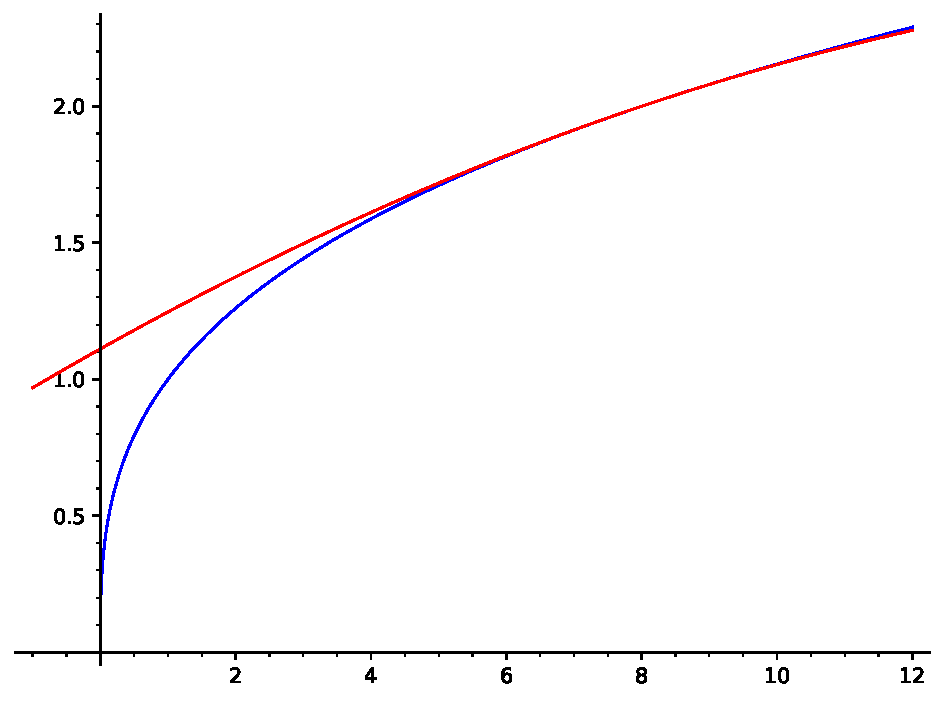
\includegraphics[width=\linewidth]{generated/sageplot/taylor.pdf}%
\end{image}%
\tcblower
\end{figureptx}%
%
\par
Para "verificar" nossas estimativas, usamos uma boa calculadora e obtemos%
\begin{align*}
\dfrac{14519}{7200}\amp = 2.01652777\ldots\\
\sqrt[3]{8.2}      \amp = 2.01652967\ldots,
\end{align*}
mostrando que a diferença entre os valores aparece somente na sexta casa decimal (\(E_2(8.2)> 1\times 10^{-6}\)), mas o dígito da diferença nessa casa não é maior ou igual a \(2\) (\(E_2(8.2)<2\times 10^{-6}\)).%
\end{divisionexercise}%
\begin{divisionexercise}{7}{}{}{exercise-teste_segder}%
Seja \(f\colon]a,b[\to\R\) uma função de classe \(\mathscr{C}^2\) e suponha que \(x_0\in]a,b[\) seja um ponto crítico de \(f\). Mostre que:%
\begin{enumerate}[label=\alph*]
\item{}se \(f'' (x_ 0)>0\), então \(x_ 0\) é um ponto de mínimo local de \(f\);%
\item{}se \(f'' (x_ 0)<0\), então \(x_ 0\) é um ponto de máximo local de \(f\).%
\end{enumerate}
%
\begin{remark}{Nota}{}{remark-teste_segder-a-b}%
Note que este é mais um caso onde a recíproca é falsa: se \(x_0\) é um ponto de mínimo local de \(f\) no interior de um intervalo aberto, não é verdade que necessariamente devemos ter \(f''(x_0)>0\). Um exemplo é o ponto \(x_0=0\) que é de mínimo para \(f(x)=x^4\).%
\end{remark}
\par\smallskip%
\noindent\textbf{\blocktitlefont Dica}.\hypertarget{hint-teste_segder-b}{}\quad{}Como fica a fórmula de Taylor de ordem \(2\) para \(f(x)\), em torno do ponto crítico \(x_0\)? Como a continuidade (preservação do sinal) de \(f''\) ajuda a fechar a questão?%
\par\smallskip%
\noindent\textbf{\blocktitlefont Solução}.\hypertarget{solution-teste_segder-c}{}\quad{}Lembrando, a fórmula de Taylor de ordem para \(f\), em torno de \(x_0\), é%
\begin{equation*}
f(x)=f(x_0)+f'(x_0)(x-x_0)+\dfrac{f''(\overline{x})}{2}(x-x_0)^2,
\end{equation*}
para algum \(\overline{x}\) entre \(x_0\) e \(x\). Como \(x_0\) é ponto crítico de \(f\), então \(f'(x_0)=0\) e a expressão acima reduz-se a%
\begin{equation}
f(x)=f(x_0)+\dfrac{f''(\overline{x})}{2}(x-x_0)^2.\label{men-taylor_crit}
\end{equation}
%
\begin{enumerate}[label=\alph*]
\item{}se \(f'' (x_ 0)>0\), então, da continuidade de \(f''\), temos que \(f'' (x)>0\), para todo \(x\) em algum intervalo aberto \(I\), contido em \(]a,b[\) e centrado em \(x_0\). Desta forma, se \(x\in I\), então, na expressão \hyperref[men-taylor_crit]{({\xreffont\ref{men-taylor_crit}})}, temos \(f''(\overline{x})>0\), donde%
\begin{equation*}
f(x)=f(x_0)+\dfrac{f''(\overline{x})}{2}(x-x_0)^2>f(x_0),
\end{equation*}
mostrando que \(x_0\) é ponto de mínimo local de \(f\).%
\item{}É um argumento análogo ao anterior, redija-o para ter certeza de que entendeu.%
\end{enumerate}
%
\end{divisionexercise}%
\end{exercises-subsection-numberless}
\end{sectionptx}
%
%
\typeout{************************************************}
\typeout{Seção 1.2 Curvas no Plano}
\typeout{************************************************}
%
\begin{sectionptx}{Seção}{Curvas no Plano}{}{Curvas no Plano}{}{}{section-sec_curvas}
%
%
\typeout{************************************************}
\typeout{Exercícios 1.2 Exercícios}
\typeout{************************************************}
%
\begin{exercises-subsection-numberless}{Exercícios}{Exercícios}{}{Exercícios}{}{}{exercises-ex_curvas}
\begin{divisionexercise}{6}{}{}{exercise-involuta}%
Um barbante é enrolado ao redor de um círculo e então desenrolado, sendo mantido esticado. A curva traçada pelo ponto \(P\) no final do barbante é chamada de \emph{involuta do círculo}. Se o círculo tiver raio \(r\) e centro \(O\), a posição inicial de \(P\) for \((r, 0)\), e se o parâmetro \(\theta\) for escolhido como na \hyperref[figure-fig_involuta]{Figura~{\xreffont\ref{figure-fig_involuta}}}, mostre que as equações paramétricas da involuta são:%
\begin{equation*}
x(\theta) = r
(\cos\theta+\theta\sin\theta)\qquad\text{e} \qquad y(\theta) =
r (\sin\theta-\theta\cos\theta).
\end{equation*}
%
\begin{sidebyside}{2}{0.05}{0.05}{0.1}%
\begin{sbspanel}{0.4}[center]%
\begin{panelfigureptx}{Figura}{A involuta do círculo.}{figure-fig_involuta}{}%
\resizebox{\linewidth}{!}{%
\begin{tikzpicture}
\draw[->] (-3,0) -- (3,0) node[below] {$x$};
\draw[->] (0,-3) -- (0,3) node[right] {$y$};
\draw[red, thick,variable=\t,domain=0:5*pi/8,samples=100]
plot ({2*(cos(\t r)+\t*sin(\t r))},{2*(sin(\t r)-\t*cos(\t r))});
\filldraw ({2*(cos(pi/3 r)+pi/3*sin(pi/3 r))},{2*(sin(pi/3
r)-pi/3*cos(pi/3 r))}) circle (2pt) node[right]{$P(\theta)$};
\draw (0,0) circle (2);
\draw[dashed] (0,0) -- ({2*cos(pi/3 r)},{2*sin(pi/3 r)})
node[above]{$T$};
\draw[dashed] ({2*cos(pi/3 r)},{2*sin(pi/3 r)}) -- ({2*(cos(pi/3
r)+pi/3*sin(pi/3 r))},{2*(sin(pi/3 r)-pi/3*cos(pi/3 r))});
\draw (1/2,0) arc (0:60:1/2) node[right,xshift=3pt]{$\theta$};
\end{tikzpicture}
}%
\tcblower
\end{panelfigureptx}%
\end{sbspanel}%
\begin{sbspanel}{0.4}[center]%
\begin{panelfigureptx}{Figura}{Uma animação desta involuta.}{figure-vid_involuta}{}%
\begin{sidebyside}{2}{0.075}{0.075}{0.17}%
\begin{sbspanel}{0.47}%
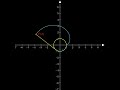
\includegraphics[width=\linewidth]{generated/youtube/video-1.jpg}
\end{sbspanel}%
\begin{sbspanel}{0.21}%

\includegraphics[width=\linewidth]{generated/qrcode/video-1.png}
\end{sbspanel}%
\end{sidebyside}%
\tcblower
\end{panelfigureptx}%
\end{sbspanel}%
\end{sidebyside}%
\par\smallskip%
\noindent\textbf{\blocktitlefont Dica}.\hypertarget{hint-involuta-b}{}\quad{}Procure triângulos retângulos semelhantes, um com a hipotenusa paralela a um dos eixos coordenados e o outro com com os catetos paralelos aos eixos. Com eles escreva essa hipotenusa e um dos catetos em termos de \(\theta\).%
\par\smallskip%
\noindent\textbf{\blocktitlefont Solução}.\hypertarget{solution-involuta-c}{}\quad{}Seguido a dica, identificamos os triângulos \(\triangle
OAT\) e \(\triangle TBP\), na figura abaixo: \begin{figureptx}{Figura}{Solução do \hyperlink{exercise-involuta}{Exercício~{\xreffont 1.2.6}}}{figure-fig_involuta_sol}{}%
\begin{image}{0.25}{0.5}{0.25}{}%
\resizebox{\linewidth}{!}{%
\begin{tikzpicture}
\draw[->] (-3,0) -- (3,0) node[below] {$x$};
\draw[->] (0,-3) -- (0,3) node[right] {$y$};
\draw[red,thick,variable=\t,domain=0:5*pi/8,samples=100]
plot ({2*(cos(\t r)+\t*sin(\t r))},{2*(sin(\t r)-\t*cos(\t r))});
\filldraw ({2*(cos(pi/3 r)+pi/3*sin(pi/3 r))},{2*(sin(pi/3
r)-pi/3*cos(pi/3 r))}) circle (2pt) node[right]{$P(\theta)$};
\draw (0,0) circle (2);
\draw[dashed] (0,0) -- ({2*cos(pi/3 r)},{2*sin(pi/3 r)})
node[above]{$T$};
\draw[dashed] ({2*cos(pi/3 r)},{2*sin(pi/3 r)}) -- ({2*(cos(pi/3
r)+pi/3*sin(pi/3 r))},{2*(sin(pi/3 r)-pi/3*cos(pi/3 r))});
\draw (1/2,0) arc (0:60:1/2) node[right,xshift=3pt]{$\theta$};
\draw[thick,blue] (0,0) node[below left]{$O$} -- ({2*cos(pi/3
r)},{2*sin(pi/3 r)}) -- ({2*cos(pi/3 r)},0)
node[below]{$A$} -- cycle;
\draw[thick,blue] ({2*cos(pi/3 r)},{2*sin(pi/3 r)}) --
({2*(cos(pi/3 r)+pi/3*sin(pi/3 r))},{2*(sin(pi/3
r)-pi/3*cos(pi/3 r))}) --
({2*cos(pi/3 r)},{2*(sin(pi/3
r)-pi/3*cos(pi/3 r))}) node[below right]{$B$} -- cycle;
\end{tikzpicture}
}%
\end{image}%
\tcblower
\end{figureptx}%
%
\par
Como os triângulos indicados são retângulos e os ângulos \(T\hat{O}A\) e \(B\hat{T}P\) são congruente e medem \(\theta\) (por que?), temos que \(B\hat{P}T\) mede \(\dfrac{\pi}{2}-\theta\). Outra observação importante é que a medida do segmento \(\overline{PT}\) é a mesma do arco da circunferência relativo ao ângulo \(\theta\), ou seja, \(m(PT)=r\theta\).%
\par
Além disso, se escrevemos \(P(\theta)=\big(x(\theta),
y(\theta)\big)\), é fácil ver que \(x(\theta)=m(OA)+m(BP)\) e \(y(\theta)=m(AT)-m(BT)\).%
\par
Da trigonometria, sabemos que%
\begin{gather*}
m(OA)=r\cos\theta;\quad
m(BP)=r\theta\cos\big(\dfrac{\pi}{2}-\theta\big)=r\theta\sin\theta;\\
m(AT)=r\sin\theta;\quad
m(BT)=r\theta\sin\big(\dfrac{\pi}{2}-\theta\big)=r\theta\cos\theta;
\end{gather*}
%
\par
Segue daí que \(x(\theta)=r(\cos\theta+\theta\sin\theta)\) e \(y(\theta)=r(\sin\theta-\theta\cos\theta)\), como desejado.%
\end{divisionexercise}%
\end{exercises-subsection-numberless}
\end{sectionptx}
%
%
\typeout{************************************************}
\typeout{Seção 1.3 Funções de duas variáveis e curvas de nível}
\typeout{************************************************}
%
\begin{sectionptx}{Seção}{Funções de duas variáveis e curvas de nível}{}{Funções de duas variáveis e curvas de nível}{}{}{section-sec_func}
%
%
\typeout{************************************************}
\typeout{Exercícios 1.3 Exercícios}
\typeout{************************************************}
%
\begin{exercises-subsection-numberless}{Exercícios}{Exercícios}{}{Exercícios}{}{}{exercises-ex_func}
\begin{divisionexercise}{7}{}{}{exercise-func_niv}%
Seja \(f(x,y)=\dfrac{2x^2+4y^2}{x^2+y^2+1}\).%
\begin{enumerate}[label=\alph*.]
\item{}Esboce as curvas de nível de \(f\) dos níveis \(c=1\), \(c=2\) e \(c=3\).%
\item{}Encontre uma curva derivável \(\gamma\), definida num intervalo \(I\subseteq\R\), cuja imagem seja a curva de nível de \(f\) do nível \(c=1\).%
\item{}Determine o vetor tangente à curva \(\gamma\), que você encontrou no item anterior, no ponto \((1,0)\).%
\item{}Seja \(\Gamma\colon [0,2\pi]\to\R^3\) dada por \(\Gamma(t)=\big(\sin t, \cos t, z(t)\big)\). Sagendo que a imagem da curva está contida no gráfico de \(f\), enconte o vetor tangente a \(\Gamma\) em \(\Gamma(\frac{\pi}{3})\).%
\end{enumerate}
%
\par\smallskip%
\noindent\textbf{\blocktitlefont Dica}.\hypertarget{hint-func_niv-b}{}\quad{}Caso precise, recorde o que é uma curva de nível e veja alguns exemplos na \hyperref[section-ap_func]{Seção~{\xreffont\ref{section-ap_func}}}. Uma dica para cada item:%
\begin{enumerate}[label=\alph*.]
\item{}Depois de escrever a equação que define cada curva de nível, é um exercício de reconhecer cônicas a partir de suas equações reduzidas.%
\item{}É o clássico caso de parametrizar uma cônica%
. \item{}Vetor tangente num ponto? É só derivar a parametrização!%
\item{}Basta lembrar que se \((x,y,z)\in Gr f\), então \(z=f(x,y)\). Para nossos propósitos, uma curva em \(\R^3\) tem as mesmas características e propriedades (continuidade, derivabilidade, etc.) de uma curva no plano, mas "com uma coordenada a mais".%
\end{enumerate}
%
\par\smallskip%
\noindent\textbf{\blocktitlefont Resposta}.\hypertarget{answer-func_niv-c}{}\quad{}%
\begin{enumerate}[label=\alph*.]
\item{}\begin{sidebyside}{2}{0.05}{0.05}{0.1}%
\begin{sbspanel}{0.3}[center]%
As curvas de nível são dadas pelas seguintes equações:%
\begin{align*}
f^{-1}(1)\colon\,& x^2+3y^2=1 \text{ (elipse)}\\
f^{-1}(2)\colon\,& y^2=1 \text{ (par de paralelas)}\\
f^{-1}(3)\colon\,& y^2-x^2=3 \text{ (hipérbole)}
\end{align*}
%
\end{sbspanel}%
\begin{sbspanel}{0.5}[center]%
\begin{panelfigureptx}{Figura}{Curvas de nível.}{figure-fig_niveis}{}%
\resizebox{\linewidth}{!}{%
\begin{tikzpicture}
\draw[->] (-3,0) -- (3,0) node[below] {$x$};
\draw[->] (0,-3) -- (0,3) node[right] {$y$};
\draw[red] (0,0) ellipse [x radius=1, y radius=1/sqrt(3)];
\draw[orange] (-2.9,1) -- (2.9,1);
\draw[orange] (-2.9,-1) -- (2.9,-1);
\draw[green,variable=\t,domain=-1.1:1.1,samples=100]
plot ({sqrt(3)*sinh(\t)},{sqrt(3)*cosh(\t)});
\draw[green,variable=\t,domain=-1.1:1.1,samples=100]
plot ({sqrt(3)*sinh(\t)},{-sqrt(3)*cosh(\t)});
\end{tikzpicture}
}%
\tcblower
\end{panelfigureptx}%
\end{sbspanel}%
\end{sidebyside}%
%
\item{}Uma possível parametrização é \(\gamma(t)=\big(\sin t,
\dfrac{\cos t}{\sqrt{3}}\big)\), \(t\in [0,2\pi]\).%
\item{}Qualquer múltiplo do vetor \(\vec{v}=(0,1)\) está correta, o que você encontrar depende da parametrização utilizada no item anterior.%
\item{}Como acima, qualquer mútiplo do vetor \(\vec{v}=\big(\dfrac{1}{2},-\dfrac{\sqrt{3}}{2},-\dfrac{\sqrt{3}}{2}\big)\) é uma resposta correta.%
\end{enumerate}
%
\par\smallskip%
\noindent\textbf{\blocktitlefont Solução}.\hypertarget{solution-func_niv-d}{}\quad{}Seguido as dicas de cada item%
\begin{enumerate}[label=\alph*.]
\item{}Observamos inicialmente que o domínio de \(f\) é todo o plano \(\R^2\). Assim, para%
\begin{itemize}[label=\textbullet]
\item{}\(c=1\): \(f(x,y)=1\iff
\dfrac{2x^2+4y^2}{x^2+y^2+1}=1\iff x^2+3y^2=1\), que descreve uma elipse centrada na origem de "raios" \(1\) e \(\dfrac{\sqrt{3}}{3}\).%
\item{}\(c=2\): \(f(x,y)=2\iff
\dfrac{2x^2+4y^2}{x^2+y^2+1}=2\iff y^2=1\), que descreve as retas paralelas \(y=1\) e \(y=-1\).%
\item{}\(c=3\): \(f(x,y)=1\iff
\dfrac{2x^2+4y^2}{x^2+y^2+1}=3\iff y^2-x^2=3\), que descreve uma hipébole com focos no eixo \(Oy\).%
\end{itemize}
Um esboço das três curvas de nível está indicado na resposta deste exercício.%
\item{}Em outras palavras, este item pede que parametrizemos o conjunto%
\begin{equation*}
f^{-1}(1)=\big\{(x,y)\in\R^2\colon
x^2+3y^2=1\big\}
\end{equation*}
%
\par
A equação \(x^2+3y^2=1\) pode ser reescrita como \(x^2+(\sqrt{3}y)^2=1\) e, portanto, podemos escrever \(x(t)=\cos t\) e \(\sqrt{3}y(t)=\sin t\iff
y(t)=\dfrac{\sin t}{\sqrt{3}}\), \(t\in[0,2\pi]\). Com este domínio a curva \(\gamma(t)=\big(\cos t,\dfrac{\sin
t}{\sqrt{3}}\big)\), descreve todos os pontos da curva de nível indicada.%
\item{}Notamos que \(f(1,0)=1\), logo \((1,0)\in
f^{-1}(1)\) e, também é fácil ver que \((1,0)=\gamma(0)\). Assim, um vetor tangente à curva no ponto indicado é \(\gamma'(0)=(0,1)\), já que \(\gamma'(t)=\big(-\sin t,\dfrac{\cos
t}{\sqrt{3}}\big)\). Observamos que qualquer múltiplo do vetor indicado também uma resposta válida.%
\item{}Dizer que a imagem de uma curva, \(\eta(t)=\big(x(t),
y(t), z(t)\big)\) está contida no gráfico de uma função \(f\colon A\subseteq\R^2\to\R\), significa exatamente dizer que \(z(t)=f\big(x(t),y(t)\big)\).%
\par
No caso deste exercício isso significa que \(z(t)=f(\sin t, \cos
t)=\dfrac{2\sin^2t+4\cos^2t}{\sin^2t+\cos^2t+1}=1+\cos^2t\).Com isso, \(\Gamma(t)=(\sin t,\cos t, 1+\cos^2t)\) e, consequente \(\Gamma'(t)=(\cos t, -\sin t, -2\cos
t\sin t)\implies
\Gamma'(t)=\big(\dfrac{1}{2},-\dfrac{\sqrt{3}}{2},-\dfrac{\sqrt{3}}{2}\big).\)%
\par
Veja nas figuras abaixo, o gráfico de \(f\), com os cortes nos níveis pedidos no primeiro item e também a imagem da curva \(\Gamma(t)\) e sua projeção no plano \(Oxy\). \begin{sidebyside}{2}{0.05}{0.05}{0.1}%
\begin{sbspanel}{0.4}[center]%
\begin{panelfigureptx}{Figura}{Gráfico de \(f\) e curvas de nível}{figure-fig_exfunca}{}%
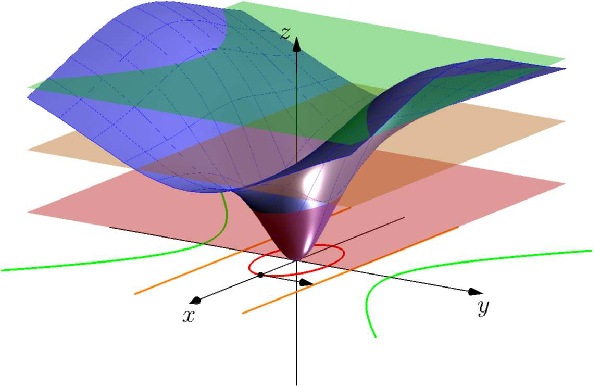
\includegraphics[width=\linewidth]{generated/asymptote/exfunca.pdf}
\tcblower
\end{panelfigureptx}%
\end{sbspanel}%
\begin{sbspanel}{0.4}[center]%
\begin{panelfigureptx}{Figura}{Gráfico de \(f\), a imagem de \(\Gamma\) e sua projeção em \(Oxy\).}{figure-fig_exfuncb}{}%
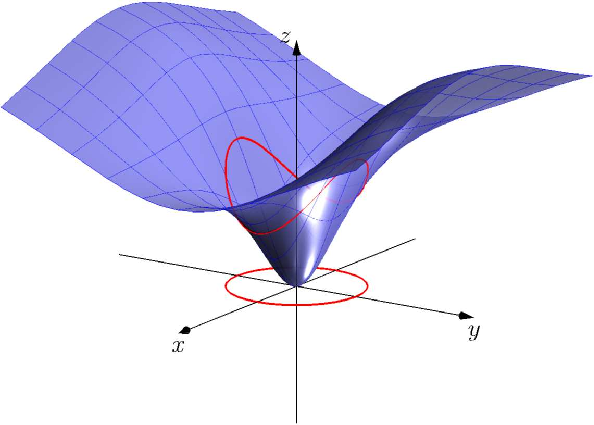
\includegraphics[width=\linewidth]{generated/asymptote/exfuncb.pdf}
\tcblower
\end{panelfigureptx}%
\end{sbspanel}%
\end{sidebyside}%
%
\end{enumerate}
%
\end{divisionexercise}%
\end{exercises-subsection-numberless}
\end{sectionptx}
%
%
\typeout{************************************************}
\typeout{Seção 1.4 Limites e Continuidade}
\typeout{************************************************}
%
\begin{sectionptx}{Seção}{Limites e Continuidade}{}{Limites e Continuidade}{}{}{section-sec_limcont}
%
%
\typeout{************************************************}
\typeout{Exercícios 1.4 Exercícios}
\typeout{************************************************}
%
\begin{exercises-subsection-numberless}{Exercícios}{Exercícios}{}{Exercícios}{}{}{exercises-ex_limcont}
\begin{divisionexercise}{1.n}{}{}{exercise-lim41n}%
Calcule, caso exista, \(\lim\limits_{(x,y)\to(0,0)}
\dfrac{x^3\big(1-\cos(x^2+y^2)\big)}{(x^2+y^2)^3}\). Justifique, caso não exista.%
\par\smallskip%
\noindent\textbf{\blocktitlefont Dica}.\hypertarget{hint-lim41n-b}{}\quad{}Como você calcularia, sem usar a regra de L'Hospital, \(\lim\limits_{x\to 0}\dfrac{1-\cos x}{x}\)?%
\par\smallskip%
\noindent\textbf{\blocktitlefont Resposta}.\hypertarget{answer-lim41n-c}{}\quad{}\(0\).%
\par\smallskip%
\noindent\textbf{\blocktitlefont Solução}.\hypertarget{solution-lim41n-d}{}\quad{}Seguindo a ideia da dica vamos multiplicar numerador e denominador por \(1+\cos(x^2+y^2)\), obtendo%
\begin{align*}
\lim\limits_{(x,y)\to(0,0)}
\dfrac{x^3\big(1-\cos(x^2+y^2)\big)}{(x^2+y^2)^3}
&=\lim\limits_{(x,y)\to(0,0)}
\dfrac{x^3\big(1-\cos^2(x^2+y^2)\big)}
{\big(1+\cos(x^2+y^2)\big)(x^2+y^2)^3}\\
&=\lim\limits_{(x,y)\to(0,0)}
x\dfrac{x^2}{x^2+y^2}\dfrac{\sin(x^2+y^2)}{x^2+y^2}
\dfrac{\sin(x^2+y^2)}{x^2+y^2}=0,
\end{align*}
pois o primeiro fator tende a \(0\), o segundo é limitado, enquanto que o terceiro e quarto (iguais) tendem a \(1\), como feito no \hyperref[example-exemplo_comp]{Exemplo~{\xreffont\ref{example-exemplo_comp}}}.%
\end{divisionexercise}%
\begin{divisionexercise}{2.c}{}{}{exercise-lim42c}%
Calcule, caso exista, \(\lim\limits_{(x,y)\to(0,0)}
x^2\ln(3x^2+y^2)\arctan\big(\dfrac{1}{y^2-x^2}\big)\). Justifique, caso não exista.%
\par\smallskip%
\noindent\textbf{\blocktitlefont Dica}.\hypertarget{hint-lim42c-b}{}\quad{}Como você calcularia, usando a regra de L'Hospital, \(\lim\limits_{x\to 0}x\ln x\)?%
\par\smallskip%
\noindent\textbf{\blocktitlefont Resposta}.\hypertarget{answer-lim42c-c}{}\quad{}\(0\).%
\par\smallskip%
\noindent\textbf{\blocktitlefont Solução}.\hypertarget{solution-lim42c-d}{}\quad{}Seguindo a ideia da dica, vamos multiplicar numerador e denominador por \(3x^2+y^2\), obtendo%
\begin{align*}
\lim\limits_{(x,y)\to(0,0)}x^2\ln(3x^2&+y^2)\arctan\big(\dfrac{1}{y^2-x^2}\big)\\
&=\lim\limits_{(x,y)\to(0,0)}
\dfrac{x^2}{3x^2+y^2}(3x^2+y^2)\ln(3x^2+y^2)\arctan\big(\dfrac{1}{y^2-x^2}\big),
\end{align*}
onde%
\begin{itemize}[label=\textbullet]
\item{}o primeiro fator é limitado (análogo ao primeiro exemplo em \hyperref[figure-vid_limitada]{Figura~{\xreffont\ref{figure-vid_limitada}}});%
\item{}usando a \hyperref[proposition-prop_comp]{Proposição~{\xreffont\ref{proposition-prop_comp}}} com \(f(t)=\begin{cases}t\ln t,& t\neq 0\\\hfill 0,&
t=0\end{cases}\) e \(g(x,y)=3x^2+y^2\), temos que o segundo tende a zero, e%
\item{}o terceiro fator é limitado, pois \(-\dfrac{\pi}{2}<\arctan(t)<\dfrac{\pi}{2}\), para todo \(t\in\R\).%
\end{itemize}
%
\par
Sendo o produto de fatores limitados também um termo limitado, o \hyperref[corollary-cor_confronto]{Corolário~{\xreffont\ref{corollary-cor_confronto}}} garante que o limite pedido vale \(0\).%
\end{divisionexercise}%
\begin{divisionexercise}{2.d}{}{}{exercise-lim42d}%
Calcule, caso exista, \(\lim\limits_{(x,y)\to(1,1)}
x^2\ln(3x^2+y^2)\arctan\big(\dfrac{1}{y^2-x^2}\big)\). Justifique, caso não exista.%
\par\smallskip%
\noindent\textbf{\blocktitlefont Dica}.\hypertarget{hint-lim42d-b}{}\quad{}Será que temos aqui uma indeterminação, como no exercício acima?%
\par\smallskip%
\noindent\textbf{\blocktitlefont Resposta}.\hypertarget{answer-lim42d-c}{}\quad{}Não existe.%
\par\smallskip%
\noindent\textbf{\blocktitlefont Solução}.\hypertarget{solution-lim42d-d}{}\quad{}Seguindo a ideia da dica, notamos que%
\begin{equation*}
\lim\limits_{(x,y)\to(1,1)}
x^2\ln(3x^2+y^2)=\ln(4).
\end{equation*}
%
\par
Para o termo \(\arctan\big(\dfrac{1}{y^2-x^2}\big)\), consideramos a curva \(\gamma(t)=(t,1)\), onde temos os limites laterais%
\begin{equation*}
\lim\limits_{t\to
1^\pm}\arctan\big(\gamma(t)\big)=\lim\limits_{t\to
1^\pm}\arctan\big(\dfrac{1}{1-t^2}\big)=\mp\frac{\pi}{2}.
\end{equation*}
O \hyperref[theorem-teo_limcurvas]{Teorema~{\xreffont\ref{theorem-teo_limcurvas}}} garante que este fator não tem limite.%
\par
Como a expressão original é composta pelo produto dos dois primeiros fatores, que tem limite não nulo, e o terceiro, que isoladamente não tem limite, o produto dos três fatores não pode ter limite.%
\end{divisionexercise}%
\end{exercises-subsection-numberless}
\end{sectionptx}
%
%
\typeout{************************************************}
\typeout{Seção 1.5 Derivadas Parciais, Diferenciabilidade e Plano Tangente}
\typeout{************************************************}
%
\begin{sectionptx}{Seção}{Derivadas Parciais, Diferenciabilidade e Plano Tangente}{}{Derivadas Parciais, Diferenciabilidade e Plano Tangente}{}{}{section-sec_derdifpt}
%
%
\typeout{************************************************}
\typeout{Exercícios 1.5 Exercícios}
\typeout{************************************************}
%
\begin{exercises-subsection-numberless}{Exercícios}{Exercícios}{}{Exercícios}{}{}{exercises-ex_derdifpt}
\begin{divisionexercise}{5}{}{}{exercise-dif5}%
Seja \(f(x,y)=\begin{cases}
\dfrac{x^3}{x^2+y^2},&(x,y)\neq(0,0)\\
\hfill 0,&(x,y)=(0,0).
\end{cases}\)%
\begin{enumerate}[label=\alph*]
\item{}Mostre que \(f\) é contínua em \((0,0)\).%
\item{}Calcule \(\dfrac{\partial f}{\partial x}(0,0)\) e \(\dfrac{\partial f}{\partial y}(0,0)\).%
\item{}\(f\) é diferenciável em \((0,0)\)?%
\item{}\(\dfrac{\partial f}{\partial x}\) e \(\dfrac{\partial f}{\partial y}\) são contínuas em \((0,0)\)?%
\end{enumerate}
%
\par\smallskip%
\noindent\textbf{\blocktitlefont Dica}.\hypertarget{hint-dif5-b}{}\quad{}Siga com o \hyperref[corollary-cor_confronto]{Corolário~{\xreffont\ref{corollary-cor_confronto}}} no primeiro item e pela definição em cada item seguinte.%
\par\smallskip%
\noindent\textbf{\blocktitlefont Resposta}.\hypertarget{answer-dif5-c}{}\quad{}%
\begin{enumerate}[label=\alph*]
\item{}Seguindo a dica é fácil.%
\item{}\(\dfrac{\partial f}{\partial x}(0,0)=1\) e \(\dfrac{\partial f}{\partial y}(0,0)=0\).%
\item{}Não.%
\item{}Não.%
\end{enumerate}
%
\par\smallskip%
\noindent\textbf{\blocktitlefont Solução}.\hypertarget{solution-dif5-d}{}\quad{}%
\begin{enumerate}[label=\alph*]
\item{}Para mostrar que \(f\) é contínua em \((0,0)\), precisamos verificar que \(\lim\limits_{(x,y)\to (0,0)}
f(x,y)=f(0,0)\). De fato,%
\begin{equation*}
\lim\limits_{(x,y)\to (0,0)} f(x,y)=
\lim\limits_{(x,y)\to (0,0)}\dfrac{x^3}{x^2+y^2}=
\lim\limits_{(x,y)\to
(0,0)}x\cdot\dfrac{x^2}{x^2+y^2}\stackrel{(\ast)}{=}0=f(0,0).
\end{equation*}
Logo, \(f\) é contínua em \((0,0)\). A igualdade \((\ast)\) segue da aplicação do \hyperref[corollary-cor_confronto]{Corolário~{\xreffont\ref{corollary-cor_confronto}}}.%
\item{}Vamos seguir pela definição, já que não é possível aplicar as regras de derivação no ponto em questão (o denominador se anula ali):%
\begin{align*}
\dfrac{\partial f}{\partial
x}(0,0)&=\lim\limits_{h\to
0}\dfrac{f(0+h,0)-f(0,0)}{h}
=\lim\limits_{h\to
0}\dfrac{\dfrac{h^3}{h^2+0^2}-0}{h}=1;\\
\dfrac{\partial f}{\partial
y}(0,0)&=\lim\limits_{k\to
0}\dfrac{f(0,0+k)-f(0,0)}{k}
=\lim\limits_{k\to
0}\dfrac{0-0}{k}=0;
\end{align*}
%
\item{}Seguindo também pela definição, com \((x_0,y_0)=(0,0)\), temos%
\begin{align*}
\lim\limits_{(h,k)\to(0,0)}
&\dfrac{f(h,k)-f(0,0)-f_x(0,0)h-f_y(0,0)k}
{\sqrt{h^2+k^2}}\\
& =\lim\limits_{(h,k)\to(0,0)}
\dfrac{\dfrac{h^3}{h^2+k^2}-h}{\sqrt{h^2+k^2}}=
\lim\limits_{(h,k)\to(0,0)}
-\dfrac{k^2}{(h^2+k^2)}\dfrac{k}{\sqrt{h^2+k^2}},
\end{align*}
que não existe. Para verificar isso, observe que o limite acima não existe (laterais distintos) ao longo da curva \(\gamma(t)=(t,t)\), conforme o \hyperref[theorem-teo_limcurvas]{Teorema~{\xreffont\ref{theorem-teo_limcurvas}}}.%
\item{}Para verificar a continuidade de qualquer função num ponto, precisamos do seu valor no ponto e numa vizinhança desse ponto. Os valores de \(f_x(0,0)\) e \(f_y(0,0)\) foram calculados no segundo item. Fora da origem podemos aplicar as regras derivação. Obtemos então%
\begin{align*}
f_x(x,y)=&\begin{cases}
\dfrac{x^4+3x^2y^2}{(x^2+y^2)^2},& (x,y)\neq (0,0)\\
\hfill 0,& (x,y)=(0,0).
\end{cases}\\
f_y(x,y)=&\begin{cases}
\dfrac{-2x^3y}{(x^2+y^2)^2},& (x,y)\neq (0,0)\\
\hfill 0,& (x,y)=(0,0).
\end{cases}
\end{align*}
A continuidade dessas funções se dará pela verificação de \(\lim\limits_{(x,y)\to (0,0)} f_x(x,y)=f_x(0,0)\) e \(\lim\limits_{(x,y)\to (0,0)}
f_y(x,y)=f_y(0,0)\). Nenhuma das duas condições é verdadeira, vamos fazer apenas a primeira. Usando mais uma vez o \hyperref[theorem-teo_limcurvas]{Teorema~{\xreffont\ref{theorem-teo_limcurvas}}}, com \(\gamma_1(t)=(t,0)\) e \(\gamma_2(t)=(0,t)\), temos%
\begin{align*}
\lim\limits_{t\to 0} f_x\big(\gamma_1(t)\big)
&=\lim\limits_{t\to 0}\dfrac{t^4}{t^4}=1\\
\lim\limits_{t\to 0} f_x\big(\gamma_2(t)\big)
&=\lim\limits_{t\to 0}\dfrac{0}{t^4}=0.
\end{align*}
Verifique também que a derivada parcial em \(y\) não é contínua na origem.%
\end{enumerate}
%
\begin{remark}{Nota}{}{remark-dif5-d-b}%
Neste exemplo, o candidato natural a plano tangente ao gráfico de \(f\) em \(\big(0,0,f(0,0)\big)=(0,0,0)\) é \(\pi\colon z=x\). É esperado que tal plano contenha todos os vetores tangentes a curvas deriváveis contidas no gráfico de \(f\), passando pela origem. Tais curvas são da forma \(\Gamma(t)=\Big(x(t),y(t),f\big(x(t),y(t)\big)\Big)\), com \(t\in I\) e com algum \(t_0\in I\) tal que \(x(t_0)=y(t_0)=0\). Considere, então%
\begin{equation*}
\Gamma(t)=\big(t,t,f(t,t)\big)=(t,t,t/2),\quad t\in\R.
\end{equation*}
É fácil ver que \(\Gamma(0)=(0,0,0)\), mas \(\Gamma'(0)=(1,1,\frac{1}{2})\not\in\pi\). Veja na figura como o plano aproxima bem o gráfico da função ao longos dos eixos, mas não sobre a curva: \begin{figureptx}{Figura}{Gráfico de função não derivável e candidato a plano tangente}{figure-fig_asymptote3d}{}%
\begin{image}{0.25}{0.5}{0.25}{}%
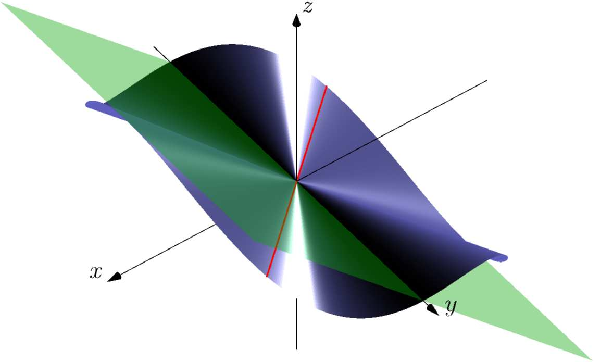
\includegraphics[width=\linewidth]{generated/asymptote/surf_level.pdf}
\end{image}%
\tcblower
\end{figureptx}%
\end{remark}
\end{divisionexercise}%
\begin{divisionexercise}{7.b}{}{}{exercise-dif7b}%
Determine o conjunto de pontos de \(\R^2\) onde \(f(x,y)=x|y|\) não é diferenciável.%
\par\smallskip%
\noindent\textbf{\blocktitlefont Dica}.\hypertarget{hint-dif7b-b}{}\quad{}Quando módulo de algo não é derivável? E um produto envolvendo módulo e uma função derivável?%
\par\smallskip%
\noindent\textbf{\blocktitlefont Resposta}.\hypertarget{answer-dif7b-c}{}\quad{}Nos pontos da forma \((a,0)\), com \(a\neq 0\).%
\par\smallskip%
\noindent\textbf{\blocktitlefont Solução}.\hypertarget{solution-dif7b-d}{}\quad{}Observamos inicialmente que podemos reescrever a função como \(f(x,y)=\begin{cases} xy,& y\geq0\\ -xy& y<0
\end{cases}.\) Com isso, é fácil ver que \(f\) é contínua em todo o plano e também de classe \(\mathscr{C}^1\) em todo ponto \((x,y)\in\R^2\) tal que \(y\neq 0\)%
\par
Logo \(f\) é diferenciável nos pontos \((x,y)\in\R^2\), \(y\neq0\).%
\par
Lembrando \(|y|\) não é derivável quando \(y=0\), precisamos de uma análise mais cuidadosa em tais pontos. Comecemos pelas derivadas parciais:%
\begin{align*}
\dfrac{\partial f}{\partial x}(x_0,0)
&=\lim\limits_{h\to 0}\dfrac{f(x_0+h,0)-f(0,0)}{h}
=\lim\limits_{h\to 0}\dfrac{(x_0+h)|0|-0}{h}=0;\\
\dfrac{\partial f}{\partial y}(x_0,0)
&=\lim\limits_{k\to 0}\dfrac{f(x_0,0+k)-f(0,0)}{k}
=\lim\limits_{k\to 0}\dfrac{x_0|k|-0}{k}.
\end{align*}
Temos dois casos a considerar:%
\begin{itemize}[label=\textbullet]
\item{}se \(x_0=0\), então \(f_x(0,0)=f_y(0,0)=0\) e a diferenciabilidade nesse ponto verifica-se rapidamente pela definição:%
\begin{equation*}
\lim\limits_{(h,k)\to(0,0)}
\dfrac{f(h,k)-f(0,0)-f_x(0,0)h-f_y(0,0)k} {\sqrt{h^2+k^2}}
=\lim\limits_{(h,k)\to(0,0)}
h\dfrac{|k|}{\sqrt{h^2+k^2}}=0, 
\end{equation*}
pois é produto de um fator que tende a zero por outro limitado (veja o \hyperref[corollary-cor_confronto]{Corolário~{\xreffont\ref{corollary-cor_confronto}}} e os exemplos em \hyperref[figure-vid_limitada]{Figura~{\xreffont\ref{figure-vid_limitada}}}).%
\item{}se \(x=x_0\neq0\), vemos que \(f_y(x_0,0)\)não existe (laterais distintos).%
\end{itemize}
%
\par
Logo \(f\) não é diferenciável nos pontos da forma \((x_0,0)\), com \(x_0\neq0\).%
\par
Veja como é o gráfico de \(f\): \begin{figureptx}{Figura}{Gráfico de \(f\).}{figure-fig_5-7b}{}%
\begin{image}{0.25}{0.5}{0.25}{}%
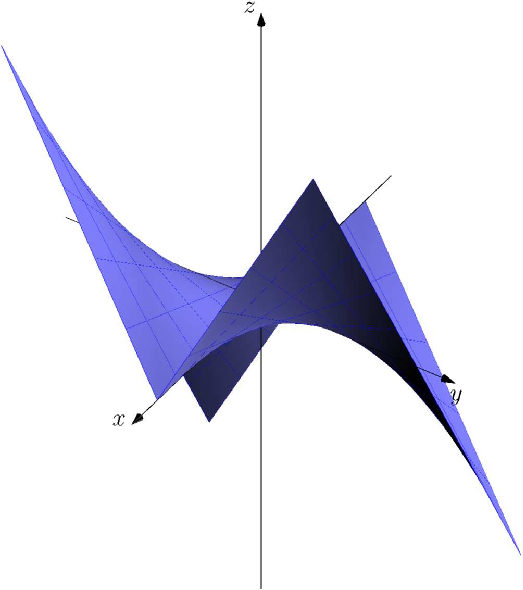
\includegraphics[width=\linewidth]{generated/asymptote/ex5-7b.pdf}
\end{image}%
\tcblower
\end{figureptx}%
%
\end{divisionexercise}%
\begin{divisionexercise}{9}{}{}{exercise-dif9}%
Mostre que os gráficos das funções \(f(x,y)=\sqrt{x^2+y^2}\) e \(g(x,y)=\frac{1}{10}(x^2+y^2)+\frac{5}{2}\) se intersectam no ponto \((3,4,5)\) e têm o mesmo plano tangente nesse ponto.%
\par\smallskip%
\noindent\textbf{\blocktitlefont Dica}.\hypertarget{hint-dif9-b}{}\quad{}Escreva as esquações dos planos tangente a cada gráfico no ponto pedido. (Talvez pergunte-se por que eles existem, para começar)%
\par\smallskip%
\noindent\textbf{\blocktitlefont Solução}.\hypertarget{solution-dif9-c}{}\quad{}Observamos inicialmente que as duas funções são de classe \(\mathscr{C}^1\) em \((3,4)\) e portanto o plano tangente está definido para ambas nesse ponto.%
\par
Como \(f(3,4)=5=g(3,4)\), então \((3,4,5)\in Gr f\bigcap
Gr g\). Para verificar que os gráficos compartilham também do mesmo plano tangente nesse ponto vamos para comparar as equações do planos tangentes. Começamos calculando as derivadas parciais:%
\begin{align*}
f_x(x,y)=\dfrac{x}{\sqrt{x^2+y^2}}\implies
f_x(3,4)=\dfrac{3}{5};&\quad
g_x(x,y)=\dfrac{x}{5}\implies
g_x(3,4)=\dfrac{3}{5};\\
f_y(x,y)=\dfrac{y}{\sqrt{x^2+y^2}}\implies
f_y(3,4)=\dfrac{4}{5};&\quad g_y(x,y)=\dfrac{y}{5}\implies
g_y(3,4)=\dfrac{4}{5};
\end{align*}
%
\par
Com isso as equações dos planos tangentes são dados por%
\begin{align*}
\pi_f\colon&
f_x(3,4)(x-3)+f_y(3,4)(y-4)-z+f(3,4)=0\implies\\
&\boxed{3(x-3)+4(x-4)-5z+25=0};\\
\pi_g\colon&
g_x(3,4)(x-3)+g_y(3,4)(y-4)-z+g(3,4)=0\implies\\
&\boxed{3(x-3)+4(x-4)-5z+25=0}.
\end{align*}
ou seja, são mesmo, como desejado.%
\par
Veja os gráficos das funções e o plano pedido. \begin{figureptx}{Figura}{Gráfico de \(f\),\(g\) e o plano tangente a ambos.}{figure-fig_5-9}{}%
\begin{image}{0.25}{0.5}{0.25}{}%
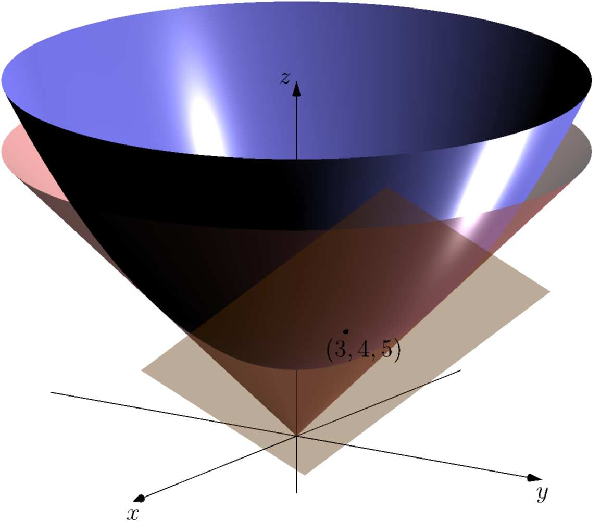
\includegraphics[width=\linewidth]{generated/asymptote/ex5-9.pdf}
\end{image}%
\tcblower
\end{figureptx}%
%
\end{divisionexercise}%
\begin{divisionexercise}{14}{}{}{exercise-dif14}%
Seja \(f(x,y)=\begin{cases}
\dfrac{xy^3}{x^2+y^2},&(x,y)\neq(0,0)\\
\hfill 0,&(x,y)=(0,0).
\end{cases}\)%
\begin{enumerate}[label=\alph*]
\item{}Verifique que \(f_y(0,y)=y\), para todo \(y\in\R\) e que \(f_x(x,0)=0\), para todo \(x\in\R\).%
\item{}Verifique que \(f_{yx}(0,0)=0\) e que \(f_{xy}(0,0)=1\).%
\end{enumerate}
%
\par\smallskip%
\noindent\textbf{\blocktitlefont Dica}.\hypertarget{hint-dif14-b}{}\quad{}É melhor fazer tudo seguindo a \hyperref[definition-def_derpar]{Definição~{\xreffont\ref{definition-def_derpar}}} e \hyperref[definition-def_derivseg]{Definição~{\xreffont\ref{definition-def_derivseg}}}.%
\par\smallskip%
\noindent\textbf{\blocktitlefont Solução}.\hypertarget{solution-dif14-c}{}\quad{}%
\begin{enumerate}[label=\alph*]
\item{}Seguindo a dica, vamos pela definição:%
\begin{align*}
f_x(0,y_0)&
=\lim\limits_{h\to0}\dfrac{f(0+h,y_0)-f(0,y_0)}{h}
=\lim\limits_{h\to0}\dfrac{hy_0^3}{h(h^2+y_0^2)}=y_0\\
f_y(x_0,0)&
=\lim\limits_{k\to0}\dfrac{f(x_0,0+k)-f(x_0,0)}{k}
=\lim\limits_{k\to0}\dfrac{x_0k^3}{k(x_0^2+k^2)}=0
\end{align*}
%
\item{}Para as segundas derivadas, usamos as expressões do item anterior:%
\begin{align*}
\dfrac{\partial^2 f}{\partial x\partial
y}(0,0)&=\lim\limits_{h\to
0}\dfrac{f_y(0+h,0)-f_y(0,0)}{h}=\lim\limits_{h\to
0}\dfrac{0-0}{h}=0;\\
\dfrac{\partial^2 f}{\partial y\partial
x}(0,0)&=\lim\limits_{k\to
0}\dfrac{f_x(0,0+k)-f_x(0,0)}{k}=\lim\limits_{h\to
0}\dfrac{k-0}{k}=1.
\end{align*}
%
\end{enumerate}
\begin{remark}{Nota}{}{remark-dif14-c-b}%
Note na figura abaixo como é quase imperceptível o fato das derivadas de mistas não coincidirem na origem. \begin{figureptx}{Figura}{Gráfico de função e cortes de nível}{figure-fig_5-14}{}%
\begin{image}{0.25}{0.5}{0.25}{}%
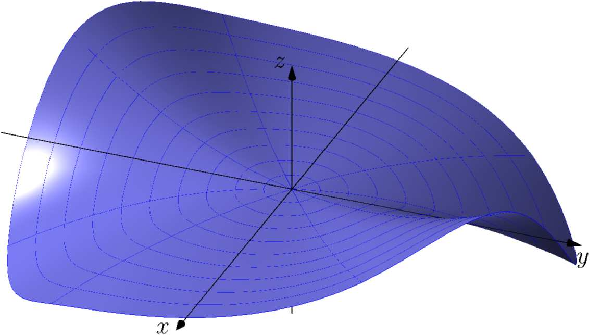
\includegraphics[width=\linewidth]{generated/asymptote/ex5-14.pdf}
\end{image}%
\tcblower
\end{figureptx}%
\end{remark}
\end{divisionexercise}%
\begin{divisionexercise}{17}{}{}{exercise-dif17}%
Sejam \(\gamma\colon\R\to\R^2\) e \(\sigma\colon\R\to\R^2\) dadas por \(\gamma(t =(1,t)\) e \(\sigma(t)=(t,0)\), para todo \(t\in\R\). Considere ainda \(F\colon\R^2\to\R\), diferenciável e tal que%
\begin{equation*}
F\big(\gamma(t)\big)=-5t^2+t+1\quad \text{e}\quad
F\big(\sigma(t)\big)=t^2, \forall t\in\R.
\end{equation*}
Dê a equação do plano tangente ao gráfico de \(F\) no ponto \((x_0,y_0)=(1,0)\).%
\par\smallskip%
\noindent\textbf{\blocktitlefont Dica}.\hypertarget{hint-dif17-b}{}\quad{}Como ficariam as derivadas parciais de \(F\) pela definição?%
\par\smallskip%
\noindent\textbf{\blocktitlefont Resposta}.\hypertarget{answer-dif17-c}{}\quad{}\(\pi\colon 2x+y-z-1=0\)%
\par\smallskip%
\noindent\textbf{\blocktitlefont Solução}.\hypertarget{solution-dif17-d}{}\quad{}Precisamos de \(F(1,0)\), \(F_x(1,0)\) e \(F_y(1,0)\) para escrever a equação do plano pedido. Como \(\gamma(0)=\sigma(1)=(1,0)\) temos que%
\begin{equation*}
\boxed{F(1,0)=F\big(\gamma(0)\big)=F\big(\sigma(1)\big)=1}.
\end{equation*}
%
\par
Seguindo a dica, temos%
\begin{align*}
F_x(1,0)&=\lim\limits_{h\to
0}\dfrac{F(1+h,0)-F(1,0)}{h}\\
&\stackrel{(\dagger)}{=}\lim\limits_{t\to
1}\dfrac{F(t,0)-F(1,0)}{t}\\
&=\lim\limits_{t\to 1}
\dfrac{F\big(\sigma(t)\big)-F\big(\sigma(1)\big)}{t-1},
\end{align*}
que é, por definição, \((F\circ\sigma)'(1)\). Como \(F\big(\sigma(t)\big)=t^2\), então \((F\circ\sigma)'(t)=2t\) e \((F\circ\gamma)'(1)=2\). Logo \(\boxed{F_x(1,0)=2}\). Em \((\dagger)\) fizemos a mudança \(t=h+1\).%
\par
Analogamente,%
\begin{align*}
F_y(1,0)&=\lim\limits_{k\to
0}\dfrac{F(1,0+k)-F(1,0)}{k}\\
&=\lim\limits_{t\to
0}\dfrac{F(1,k)-F(1,0)}{t},
\end{align*}
que é, por definição, \((F\circ\gamma)'(0)\). Como \(F\big(\gamma(t)\big)=-5t^2+t+1\), então \((F\circ\gamma)'(t)=-10t+1\) e \((F\circ\gamma)'(0)=1\). Logo \(\boxed{F_y(1,0)=1}\).%
\par
Com isso, o plano procuração tem equação%
\begin{equation*}
\pi\colon
F_x(1,0)(x-1)+F_y(1,0)(y-0)-z+F(1,0)=0\implies\boxed{2x+y-1=0}.
\end{equation*}
%
\begin{remark}{Nota}{}{remark-dif17-d-e}%
A hipótese de diferenciabilidade permitiu determinar o plano tangente ao seu gráfico conhecendo seus valores apenas ao longo de retas paralelas aos eixos coordenados que passam por \((1,0)\). Em outras palavras, quaisquer duas funções diferenciáveis que, num dado ponto, tenham os mesmos cortes de seus gráficos por planos paralelos a \(Oxz\) e \(Oyz\), que contenham o ponto \((x_0,y_0,0)\), terão o mesmo plano tangente nesse ponto. Uma figura para ilustrar: \begin{figureptx}{Figura}{Cortes do gráfico de \(F\) e o plano tangente determinado por eles.}{figure-fig_5-17}{}%
\begin{image}{0.25}{0.5}{0.25}{}%
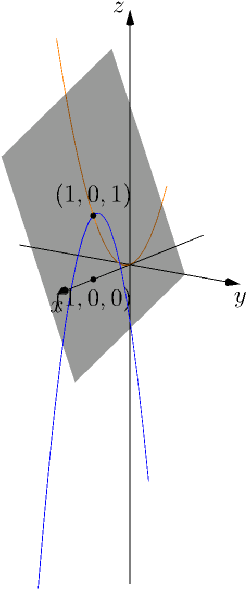
\includegraphics[width=\linewidth]{generated/asymptote/ex5-17.pdf}
\end{image}%
\tcblower
\end{figureptx}%
\end{remark}
Com o desenvolvimento dos conteúdos veremos que, conhecendo os cortes do gráfico de uma função por dois planos verticais não paralelos passando por um ponto desse gráfico, determinamos o plano tangente ao gráfico nesse ponto.%
\end{divisionexercise}%
\end{exercises-subsection-numberless}
\end{sectionptx}
%
%
\typeout{************************************************}
\typeout{Seção 1.6 Regras da Cadeia}
\typeout{************************************************}
%
\begin{sectionptx}{Seção}{Regras da Cadeia}{}{Regras da Cadeia}{}{}{section-sec_cadeia}
%
%
\typeout{************************************************}
\typeout{Exercícios 1.6 Exercícios}
\typeout{************************************************}
%
\begin{exercises-subsection-numberless}{Exercícios}{Exercícios}{}{Exercícios}{}{}{exercises-ex_cadeia}
\begin{divisionexercise}{2}{}{}{exercise-cadeia2}%
Sejam \(f\colon\mathbb R^2\to\R\) diferenciável em \(\R^2\), com \(\nabla f(-2,-2)=(a,-4)\) e%
\begin{equation*}
g(t)=f(2t^3-4t, t^4-3t).
\end{equation*}
Determine \(a\) para que a reta tangente ao gráfico de \(g\) no ponto de abscissa \(1\) seja paralela à reta \(y=2x+3\).%
\par\smallskip%
\noindent\textbf{\blocktitlefont Dica}.\hypertarget{hint-cadeia2-b}{}\quad{}Você consegue ver \(g(t)\) como uma composta para aplicar a regra da cadeia? E mais: qual a condição para que duas retas sejam paralelas?%
\par\smallskip%
\noindent\textbf{\blocktitlefont Resposta}.\hypertarget{answer-cadeia2-c}{}\quad{}\(a=3\)%
\par\smallskip%
\noindent\textbf{\blocktitlefont Solução}.\hypertarget{solution-cadeia2-d}{}\quad{}A reta tangente ao gráfico de \(g\) no ponto de abscissa \(1\) ser paralela à reta \(y=2x+3\) significa que \(g'(1)=2\) (retas paralelas têm o mesmo coeficiente angular e o coeficiente angular da reta tangente ao gráfico de uma função real derivável é o valor de sua derivada no ponto de tangência).%
\par
Isto posto, notamos que \(g(t)=f\big(\gamma(t)\big)\), onde \(\gamma(t)=(2t^3-4t, t^4-3t)\). Usando o \hyperref[theorem-teo_cadeia]{Teorema~{\xreffont\ref{theorem-teo_cadeia}}} e as observações iniciais, temos que%
\begin{equation*}
2=g'(1)=\Big\langle \nabla
f\big(\gamma(1)\big),\gamma'(1)\Big\rangle.
\end{equation*}
%
\par
Como \(\gamma(1)=(-2,-2)\) e \(\gamma'(t)=(6t^2-4,4t^3-3)\implies \gamma'(1)=(2,1)\), temos%
\begin{equation*}
2=\big\langle \nabla
f(-2,-2),(2,1)\big\rangle=2a-4\implies \boxed{a=3}.
\end{equation*}
%
\end{divisionexercise}%
\begin{divisionexercise}{6}{}{}{exercise-cadeia6}%
Seja \(u=u(x,y)\) função de classe \(\mathscr{C}^2\) em \(\R^2\) e defina \(v(r,\theta)=u(r\cos\theta,r\sin\theta)\). Verifique que%
\begin{equation*}
\dfrac{\partial^2 v}{\partial
r^2}(r,\theta)+\dfrac{1}{r}\dfrac{\partial v}{\partial
r}(r,\theta)+\dfrac{1}{r^2}\dfrac{\partial^2
v}{\partial\theta^2}(r,\theta)=\Delta
u(r\cos\theta,r\sin\theta),
\end{equation*}
sendo \(\Delta u = u_{xx} +
u_{yy}\) , o Laplaciano em coordenadas cartesianas da função \(u\).%
\par\smallskip%
\noindent\textbf{\blocktitlefont Dica}.\hypertarget{hint-cadeia6-b}{}\quad{}Aplicação direta da Regra da Cadeia na segunda derivada, veja a fórmula \hyperref[mrow-eq_cadeiadersegc2]{({\xreffont\ref{mrow-eq_cadeiadersegc2}})}.%
\par\smallskip%
\noindent\textbf{\blocktitlefont Solução}.\hypertarget{solution-cadeia6-c}{}\quad{}Basta aplicar (com calma e coragem!) a Regra da Cadeia, usando que%
\begin{equation*}
x(r,\theta)=r\cos\theta\quad\text{e}\quad
y(r,\theta)=r\sin\theta.
\end{equation*}
Escrevendo, apenas desta vez, todos os pontos de aplicação, temos%
\begin{equation*}
\dfrac{\partial v}{\partial r}(r,\theta)
=\dfrac{\partial u}{\partial x}(r\cos\theta,r\sin\theta)
\dfrac{\partial x}{\partial r}(r,\theta)+
\dfrac{\partial u}{\partial y}(r\cos\theta,r\sin\theta)
\dfrac{\partial y}{\partial r}(r,\theta).
\end{equation*}
Sinteticamente, temos%
\begin{equation}
v_r=u_x\cos\theta+u_y\sin\theta.\label{men-cadeia6_vr}
\end{equation}
%
\par
Derivando mais uma vez em \(\theta\), usamos a regra do produto em cada parcela e também a cadeia:%
\begin{equation*}
v_{rr}=(u_{xx}\cos\theta+u_{xy}\sin\theta)\cos\theta 
+(u_{yx}\cos\theta+u_{yy}\sin\theta)\sin\theta,
\end{equation*}
ou seja,%
\begin{equation}
v_{rr}=u_{xx}\cos^2\theta+
u_{yy}\sin^2\theta+2u_{xy}\sin\theta\cos\theta,\label{men-cadeia6_vrr}
\end{equation}
pois \(u\) é uma função de classe \(\mathscr{C}^2\) (veja o \hyperref[theorem-teo_schwarz]{Teorema~{\xreffont\ref{theorem-teo_schwarz}}}).%
\par
Agora, derivando em \(\theta\):%
\begin{equation*}
v_\theta =
u_xx_\theta+u_yy_\theta=-u_xr\sin\theta+u_yr\cos\theta,
\end{equation*}
e mais uma vez%
\begin{align*}
v_{\theta\theta}=(-u_{xx}r\sin&\theta+u_{xy}r\cos\theta)(-r\sin\theta)-u_xr\cos\theta\\
&+(-u_{yx}r\sin\theta+u_{yy}r\cos\theta)r\cos\theta-u_yr\sin\theta,
\end{align*}
ou seja,%
\begin{equation}
v_{\theta\theta}=u_{xx}r^2\sin^2\theta+
u_{yy}r^2\cos^2\theta-2u_{xy}r^2\cos\theta\sin\theta-
u_xr\cos\theta-u_yr\sin\theta.\label{men-cadeia6_vtt}
\end{equation}
%
\par
Dividindo \hyperref[men-cadeia6_vtt]{({\xreffont\ref{men-cadeia6_vtt}})} por \(r^2\), \hyperref[men-cadeia6_vr]{({\xreffont\ref{men-cadeia6_vr}})} por \(r\) e somando com \hyperref[men-cadeia6_vrr]{({\xreffont\ref{men-cadeia6_vrr}})}, temos%
\begin{equation*}
v_{rr}+\dfrac{v_r}{r}+\dfrac{v_{\theta\theta}}{r^2}=u_{xx}+u_{yy},
\end{equation*}
como desejado.%
\end{divisionexercise}%
\begin{remark}{Nota}{}{remark-ex_cadeia-c}%
O sistema de coordenadas \((r,\theta)\), apresentado no \hyperlink{exercise-cadeia6}{Exercício~{\xreffont 1.6.6}}, é chamado de \emph{sistema de coordenadas polares}, como pólo na origem. As relações \(x=r\cos\theta\) e \(y=r\sin\theta\) podem ser visualizadas na figura abaixo. \begin{figureptx}{Figura}{Coordenadas polares e cartesianas.}{figure-fig_polares}{}%
\begin{image}{0.05}{0.9}{0.05}{}%
\resizebox{\linewidth}{!}{%
\begin{tikzpicture}
\filldraw[fill=green,fill opacity=0.25,draw=red, dashed] (-4.5,0) rectangle (-2.5,1.5);
\draw[->] (-5,0) -- (-2,0) node[below] {$r$};
       \draw[->] (-4.5,-.5) -- (-4.5,2) node[right] {$\theta$};
\filldraw (-3.5,1) circle (1pt);
\draw[orange] (-2.5,1) -- (-4.5,1) node[left,black]{$\theta_0$};
\draw[blue] (-3.5,1.5)--(-3.5,0) node[below,black]{$r_0$};

\filldraw[fill=green,fill opacity=0.25,draw=red, dashed] (1.5,0) circle (1);
\draw[->] (-.5,0) -- (3.5,0) node[below] {$x$};
       \draw[->] (1.5,-2) -- (1.5,2) node[right] {$y$};
       \filldraw ({1.5-sqrt(2)/4},{-sqrt(2)/4}) circle (1pt);
\draw[blue] (1.5,0) circle (1/2);
\draw[orange] (1.5,0) -- ({1.5-sqrt(2)/2},{-sqrt(2)/2});
\end{tikzpicture}
}%
\end{image}%
\tcblower
\end{figureptx}%
%
\par
Uma aplicação interessante desse sistema é a numeração das rodovias radiais e transversais do estado de São Paulo, como pode ser verificado nas páginas 11 e 12 deste \href{https://www.der.sp.gov.br/Website/Arquivos/MALHARODOVIARIA/codificacao.pdf}{documento}\footnotemark{}.%
\end{remark}
\footnotetext[1]{\nolinkurl{der.sp.gov.br/Website/Arquivos/MALHARODOVIARIA/codificacao.pdf}\label{fn-ex_cadeia-c-b-b}}%
\end{exercises-subsection-numberless}
\end{sectionptx}
%
%
\typeout{************************************************}
\typeout{Seção 1.7 Vetor Gradiente e Derivada direcional}
\typeout{************************************************}
%
\begin{sectionptx}{Seção}{Vetor Gradiente e Derivada direcional}{}{Vetor Gradiente e Derivada direcional}{}{}{section-sec_grad-dir}
%
%
\typeout{************************************************}
\typeout{Exercícios 1.7 Exercícios}
\typeout{************************************************}
%
\begin{exercises-subsection-numberless}{Exercícios}{Exercícios}{}{Exercícios}{}{}{exercises-ex_grad-dir}
\begin{divisionexercise}{4}{}{}{exercise-grad-dir4}%
Considere uma função \(f\colon \R^2 \to \R\) de classe \(\mathscr{C}^1\). Suponha que:%
\begin{enumerate}[label=\roman*]
\item{}a imagem da curva plana \(\gamma(t)=\big(\cot (t), \sec^2
(t)\big)\), para \(t \in ]0, \pi/2 [\), esteja contida numa curva de nível de \(f\);%
\item{}a imagem da curva no espaço \(\sigma(u)
=\Big(\sqrt[3]{u}, u^2+1, \dfrac{u^3}{2} -
\dfrac{\sqrt[3]{u}}{2} +1\Big)\), com \(u>0\), esteja contida no gráfico de \(f\).%
\end{enumerate}
%
\par
%
\begin{enumerate}[label=\alph*]
\item{}Determine \(\nabla f(1,2)\).%
\item{}Calcule \(\dfrac{\partial f}{\partial
\vec{v}}(1,2)\), onde \(\vec{v} = \Big( \dfrac{1}{2},
\dfrac{\sqrt{3}}{2}\Big)\).%
\item{}Determine uma equação do plano tangente ao gráfico de \(f\) no ponto \(\big(1,2,f(1,2)\big)\).%
\end{enumerate}
%
\par\smallskip%
\noindent\textbf{\blocktitlefont Dica}.\hypertarget{hint-grad-dir4-b}{}\quad{}Em itens:%
\begin{enumerate}[label=\alph*.]
\item{}Use a Regra da Cadeia para derivar compostas de \(f\) com certas curvas convenientes.%
\item{}Lembre-se, sob certas condições, da relação entre o gradiente de \(f\) e suas derivadas direcionais.%
\item{}Os ingredientes necessários para construir o plano tangente ao gráfico de \(f\) em \(\big(1,2,f(1,2)\big)\) são \(f(1,2)\) e \(\nabla f(1,2)\).%
\end{enumerate}
%
\par\smallskip%
\noindent\textbf{\blocktitlefont Resposta}.\hypertarget{answer-grad-dir4-c}{}\quad{}%
\begin{enumerate}[label=\alph*]
\item{}\(\nabla f(1,2)=\Big(1, \frac{1}{2}\Big)\).%
\item{}\(\dfrac{\partial f}{\partial \vec{v}}(1,2) =
\dfrac{2+\sqrt{3}}{4}\).%
\item{}\(2x+y-2x-2=0\).%
\end{enumerate}
%
\par\smallskip%
\noindent\textbf{\blocktitlefont Solução}.\hypertarget{solution-grad-dir4-d}{}\quad{}%
\begin{enumerate}[label=(\alph*)]
\item{}Observamos primeiramente que \(f\) é diferenciável (veja o \hyperref[theorem-teo_diff-c1]{Teorema~{\xreffont\ref{theorem-teo_diff-c1}}}) e \(\gamma, \sigma\) são curvas deriváveis. Consideramos então a função composta \(g\colon ]0, \pi/2[\to\R\) dada por \(g(t) = f\big(\gamma(t)\big)\). A condição (i) diz \(g\) é constante e então, derivando e aplicando o \hyperref[corollary-cor_cadeiagradniv]{Corolário~{\xreffont\ref{corollary-cor_cadeiagradniv}}}, obtemos%
\begin{equation*}
0=\left\langle
\nabla f(\gamma(t)) , \gamma'(t)\right\rangle = \left\langle
\nabla f(\gamma(t)) , \left(-\csc^2 (t), 2\sec^2(t)
\tan(t)\right)\right\rangle, \forall t \in ]0,
\pi/2[.
\end{equation*}
%
\par
Em particular, para \(t=\pi/4\), temos%
\begin{equation*}
\left\langle \nabla f(1,2) , (-2,4) \right\rangle = 0
\implies \boxed{\dfrac{\partial f}{\partial x}(1,2) = 2
\frac{\partial f}{\partial y}(1,2)}.
\end{equation*}
%
\par
Por outro lado, de acordo com a condição (ii), sabemos que%
\begin{equation}
\frac{u^3}{2} - \frac{\sqrt[3]{u}}{2} +1 = f\big(\sqrt[3]{u}, u^2+1\big), \forall u >0.\label{men-grad-dir4-eq1}
\end{equation}
%
\par
Usando a Regra da Cadeia (\hyperref[theorem-teo_cadeia]{Teorema~{\xreffont\ref{theorem-teo_cadeia}}}), derivamos os dois membros em relação a \(u\), concluindo que%
\begin{equation*}
\frac{3u^2}{2} - \frac{1}{6\sqrt[3]{u^2}} =
\left\langle \nabla f(\sqrt[3]{u}, u^2+1) ,
\Big(\frac{1}{3\sqrt[3]{u^2}},2u\Big)\right\rangle,
\forall u > 0.
\end{equation*}
%
\par
Tomando \(u=1\), obtemos%
\begin{equation*}
\frac{8}{6} =
\left\langle \nabla f(1,2) ,
\Big(\frac{1}{3},2\Big)\right\rangle \implies
\boxed{\frac{\partial f}{\partial x}(1,2) + 6\frac{\partial
f}{\partial y}(1,2) = 4}.
\end{equation*}
Logo, usando as equações para as derivadas parciais em destaque, \(\nabla f(1,2) = \Big(
1 , \dfrac{1}{2}\Big)\).%
\item{}Como \(f\) é diferenciável, usamos a \hyperref[proposition-prop_derdir]{Proposição~{\xreffont\ref{proposition-prop_derdir}}} para calcular a derivada direcional:%
\begin{equation*}
\dfrac{\partial f}{\partial \vec{v}}(1,2) = \big\langle
\nabla f(1,2), \vec{v}\big\rangle =
\frac{2+\sqrt{3}}{4}.
\end{equation*}
%
\item{}Fazendo \(u=1\) na equação , encontramos \(f(1,2)=1\). Deste modo, o plano desejado tem equação%
\begin{equation*}
\dfrac{\partial f}{\partial
x}(1,2)(x-1) + \frac{\partial f}{\partial
y}(1,2)(y-2)-z+f(1,2)=0,
\end{equation*}
ou seja, \(2x+y-2z-2=0\).%
\end{enumerate}
%
\par
Para enxergar geometricamente o que acontece, notamos que \(1=f(1,2)=\gamma(\pi/4)\) e, como a curva \(\gamma\) tem sua imagem contida numa curva de nível de \(f\), então tal curva é a curva de nível \(1\). Com isso a curva \(\Gamma(t)=\big(\cot (t), \sec^2 (t),1\big)\) tem sua imagem contida no gráfico de \(f\), assim como a imagem de \(\sigma\), conforme a hipótese (ii).%
\par
A função \(f\) é de classe \(\mathscr{C}^1\) (portanto diferenciável) e seus valores são conecidos ao longo de duas curvas no domínio, a saber \(\gamma\) e a projeção de \(\sigma\) no plano \(Oxy\), dada por \(\hat\sigma(u)=(\sqrt[3]{u},u^2+1)\). Isso, aliado ao fato de \(\Gamma'(\pi/4)\) e \(\sigma'(1)\) serem linearmente independentes, determinam o plano tangente ao gráfico de \(f\) no ponto \(\big(1,2,f(1,2)\big)\), que aquele que contém as retas tangentes a \(\Gamma\) e \(\sigma\) em \(\big(1,2,f(1,2)\big)\), onde se interceptam. Tudo isso é feito sem saber o valor de \(f\) nos demais pontos do seu domínio.%
\par
Em outras palavras, o plano tangente a qualquer que seja a superfície (gráfico de uma função a duas variáveis) que contenha estas duas curvas é sempre o mesmo!%
\begin{figureptx}{Figura}{Cortes do gráfico de \(f\) e o plano tangente determinado por eles.}{figure-fig_2-4}{}%
\begin{image}{0}{1}{0}{}%
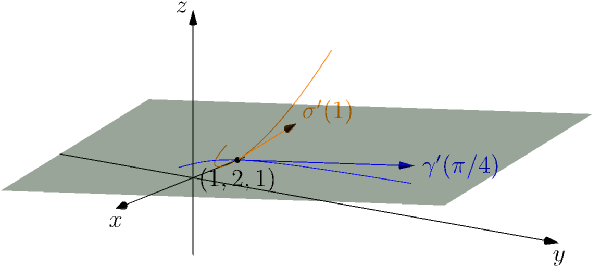
\includegraphics[width=\linewidth]{generated/asymptote/ex2-4.pdf}
\end{image}%
\tcblower
\end{figureptx}%
\end{divisionexercise}%
\begin{divisionexercise}{8}{}{}{exercise-grad-dir8}%
Mostre que \(f(x,y) = \sqrt[3]{x^2y}\) é contínua em \((0,0)\) e tem todas as derivadas direcionais em \((0,0)\). A função \(f\) é diferenciável em \((0,0)\)?%
\par\smallskip%
\noindent\textbf{\blocktitlefont Dica}.\hypertarget{hint-grad-dir8-b}{}\quad{}Use a definição para calcular as derivadas direcionais e compare com a \hyperref[proposition-prop_derdir]{Proposição~{\xreffont\ref{proposition-prop_derdir}}}.%
\par\smallskip%
\noindent\textbf{\blocktitlefont Resposta}.\hypertarget{answer-grad-dir8-c}{}\quad{}\(f\) não é diferenciável em \((0,0)\).%
\par\smallskip%
\noindent\textbf{\blocktitlefont Solução}.\hypertarget{solution-grad-dir8-d}{}\quad{}Notemos que \(f\) é composta de funções contínuas (raiz cúbica e função polinomial), de modo que \(f\) é contínua em todos os pontos de seu domínio (todo o plano \(\R^2\)). Para calcular as derivadas direcionais em \((0,0)\), procedemos usando a \hyperref[definition-def_derdir]{Definição~{\xreffont\ref{definition-def_derdir}}}: se \(\vec{v}= (h,k)\) é um vetor unitário, então%
\begin{equation}
\dfrac{\partial f}{\partial \vec{v}}(0,0)= \lim_{t \to 0}
\frac{f((0,0)+t\vec{v}) - f(0,0)}{t} = \lim_{t \to 0}
\frac{\sqrt[3]{t^3h^2k}}{t} = \sqrt[3]{h^2k}.\label{men-eq2_8}
\end{equation}
%
\par
Embora todas as derivadas direcionais de \(f\) em \((0,0)\) existam, \(f\) não é diferenciável neste ponto. De fato, aplicando \hyperref[men-eq2_8]{({\xreffont\ref{men-eq2_8}})} para os vetores \(e_1=(1,0)\), \(e_2=(0,1)\) e \(\vec{v} = \left(
\frac{\sqrt{2}}{2}, \frac{\sqrt{2}}{2}\right)\), obtemos%
\begin{equation*}
\dfrac{\partial f}{\partial x}(0,0) = \frac{\partial
f}{\partial e_1}(0,0) = 0, \quad \frac{\partial f}{\partial
y}(0,0) = \frac{\partial f}{\partial e_2}(0,0) = 0 \quad
\text{e} \quad \frac{\partial f}{\partial \vec{v}}(0,0) =
\frac{\sqrt{2}}{2}.
\end{equation*}
Isto implica que%
\begin{equation*}
\left\langle
\nabla f(0,0), \vec{v}\right \rangle = 0 \neq \frac{\sqrt{2}}{2}
=\frac{\partial f}{\partial \vec{v}}(0,0)
\end{equation*}
e, portanto, \(f\) não é diferenciável em \((0,0)\).%
\begin{remark}{Nota}{}{remark-grad-dir8-d-c}%
O fato de \hyperref[men-eq2_8]{({\xreffont\ref{men-eq2_8}})} não ser linear nas variáveis \(h,k\) já implica, como indicado após a  que \(f\) não pode ser diferenciável em \((0,0)\). De fato, se \(f\) fosse diferenciável em \((0,0)\), com \(\nabla f(0,0)=(A,B)\), teríamos%
\begin{equation*}
\dfrac{\partial f}{\partial \vec{v}}(0,0) = \left\langle
\nabla f(0,0), (h,k)\right\rangle = Ah + Bk,
\end{equation*}
uma aplicação linear de \(\R^2\) em \(\R\), usualmente denotada por \(Df_{(x_0,y_0)}\colon\R^2\to\R\), dada por \(Df_{(x_0,y_0)}(\vec{v})=\langle\nabla
f(x_0,y_0),\vec{v}\rangle\).\end{remark}
\begin{figureptx}{Figura}{O gráfico de \(f\).}{figure-fig_2-8}{}%
\begin{image}{0}{1}{0}{}%
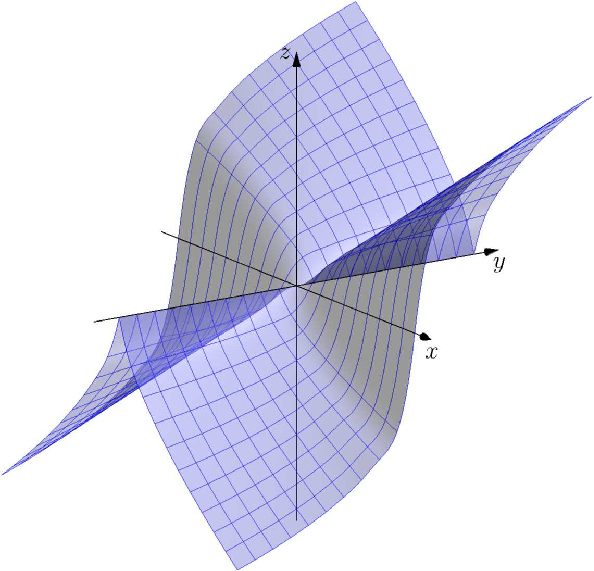
\includegraphics[width=\linewidth]{generated/asymptote/ex2-8.pdf}
\end{image}%
\tcblower
\end{figureptx}%
\end{divisionexercise}%
\end{exercises-subsection-numberless}
\end{sectionptx}
%
%
\typeout{************************************************}
\typeout{Seção 1.8 Curvas no \(\R^3\)}
\typeout{************************************************}
%
\begin{sectionptx}{Seção}{Curvas no \(\R^3\)}{}{Curvas no \(\R^3\)}{}{}{section-sec_curvasR3}
%
%
\typeout{************************************************}
\typeout{Exercícios 1.8 Exercícios}
\typeout{************************************************}
%
\begin{exercises-subsection-numberless}{Exercícios}{Exercícios}{}{Exercícios}{}{}{exercises-ex_curvasR3}
\begin{divisionexercise}{2.a}{}{}{exercise-curvasR3-2a}%
Determine uma parametrização para a curva%
\begin{equation*}
C = \big\{
(x,y,z) \in \R^3\colon x^2+y^2=z\text{ e }z=2y\big\}.
\end{equation*}
%
\par\smallskip%
\noindent\textbf{\blocktitlefont Dica}.\hypertarget{hint-curvasR3-2a-b}{}\quad{}Substitua uma equação na outra e complete quadrados.%
\par\smallskip%
\noindent\textbf{\blocktitlefont Resposta}.\hypertarget{answer-curvasR3-2a-c}{}\quad{}Uma parametrização é \(\gamma\colon\R\to\R^3\) dada por \(\gamma(t) = \big( \cos t, \sin t + 1 , 2 \sin t +
2\big)\).%
\par\smallskip%
\noindent\textbf{\blocktitlefont Solução}.\hypertarget{solution-curvasR3-2a-d}{}\quad{}Substituindo \(z=2y\) em \(z = x^2 + y^2\), obtemos \(x^2 + y^2 - 2y = 0\). Completando quadrados, encontramos \(x^2 + (y-1)^2 = 1\), de modo que podemos escrever \(x =
\cos t\) e \(y-1 = \sin t\). Desta forma, a curva \(\gamma\colon\R\to\R^3\) dada por%
\begin{equation*}
\gamma(t) = \big( \cos
t, \sin t + 1 , 2 \sin t + 2\big)
\end{equation*}
é uma parametrização de \(C\).%
\begin{figureptx}{Figura}{A interseção das duas superfícies em destaque.}{figure-fig_3-2a}{}%
\begin{image}{0}{1}{0}{}%
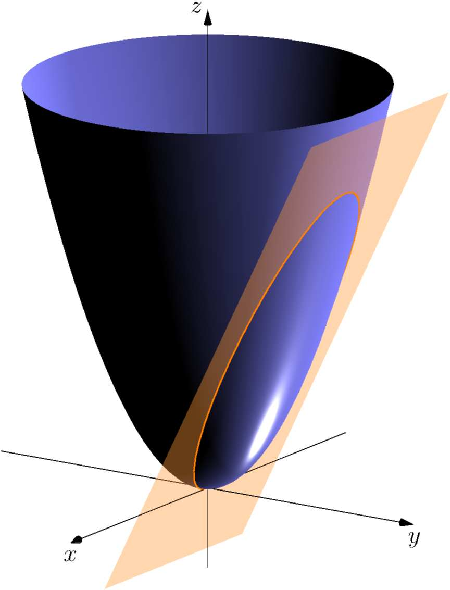
\includegraphics[width=\linewidth]{generated/asymptote/ex3-2a.pdf}
\end{image}%
\tcblower
\end{figureptx}%
Analise as coordenadas da paramentrização e veja como são as projeções da curva em cada plano coordenado. Note também que o intervalo da parametrização poderia ser \([0,2\pi]\), que cobriria apenas "uma volta completa" na curva.%
\end{divisionexercise}%
\begin{divisionexercise}{2.d}{}{}{exercise-curvasR3-2d}%
Determine uma parametrização para a curva%
\begin{equation*}
C = \big\{
(x,y,z)\in\R^3\colon x>0, x^2+y^2 -z^2= 4\text{ e
}z=x+y\big\}.
\end{equation*}
%
\par\smallskip%
\noindent\textbf{\blocktitlefont Dica}.\hypertarget{hint-curvasR3-2d-b}{}\quad{}Substitua uma equação na outra e lembre-se da condição \(x>0\).%
\par\smallskip%
\noindent\textbf{\blocktitlefont Resposta}.\hypertarget{answer-curvasR3-2d-c}{}\quad{}Uma parametrização é \(\gamma\colon]0,+\infty[\to\R^3\) dada por \(\gamma(t) =
\Big(t,-\dfrac{2}{t},\dfrac{t^2-2}{t}\Big)\).%
\par\smallskip%
\noindent\textbf{\blocktitlefont Solução}.\hypertarget{solution-curvasR3-2d-d}{}\quad{}Substituindo \(z=x+y\) em \(x^2 + y^2 - z^2 =4\), obtemos%
\begin{equation*}
x^2 + y^2 -(x+y)^2 = 4 \implies -2xy = 4 \implies y
= - \frac{2}{x}
\end{equation*}
e \(z = x+ y = \dfrac{x^2-2}{x}\). Como queremos \(x>0\), podemos tomar a curva \(\gamma\colon]0,+\infty[ \to\R^3\) dada por%
\begin{equation*}
\gamma(t)=\Big(t, - \frac{2}{t}, \frac{t^2-2}{t}\Big).
\end{equation*}
%
\begin{figureptx}{Figura}{A interseção das duas superfícies em destaque.}{figure-fig_3-2d}{}%
\begin{image}{0}{1}{0}{}%
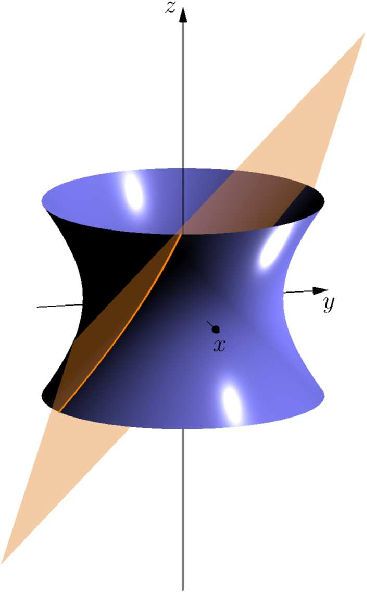
\includegraphics[width=\linewidth]{generated/asymptote/ex3-2d.pdf}
\end{image}%
\tcblower
\end{figureptx}%
\end{divisionexercise}%
\end{exercises-subsection-numberless}
\end{sectionptx}
%
%
\typeout{************************************************}
\typeout{Seção 1.9 Superfícies de nível, planos tangente e derivadas direcionais}
\typeout{************************************************}
%
\begin{sectionptx}{Seção}{Superfícies de nível, planos tangente e derivadas direcionais}{}{Superfícies de nível, planos tangente e derivadas direcionais}{}{}{section-sec_supptddir}
%
%
\typeout{************************************************}
\typeout{Exercícios 1.9 Exercícios}
\typeout{************************************************}
%
\begin{exercises-subsection-numberless}{Exercícios}{Exercícios}{}{Exercícios}{}{}{exercises-ex_supptddir}
\begin{divisionexercise}{3}{}{}{exercise-supptdir-3}%
Seja \(a>0\) e considere o plano tangente à superfície \(xyz=a\) num ponto do primeiro octante. Mostre que o tetraedro formado por este plano e os planos coordenados tem volume independente do ponto de tangência.%
\par\smallskip%
\noindent\textbf{\blocktitlefont Dica}.\hypertarget{hint-supptdir-3-b}{}\quad{}Escreva a equação do plano tangente à superfície dada num ponto \((x_0,y_0,z_0)\) arbitrário do primeiro octante, encontre os vértices do tetraedro pedido e calcule seu volume.%
\par\smallskip%
\noindent\textbf{\blocktitlefont Resposta}.\hypertarget{answer-supptdir-3-c}{}\quad{}O volume do tetraedro pedido é igual a \(\dfrac{9a}{2}\).%
\par\smallskip%
\noindent\textbf{\blocktitlefont Solução}.\hypertarget{solution-supptdir-3-d}{}\quad{}Seguindo o contexto da \hyperref[definition-def_planotangente]{Definição~{\xreffont\ref{definition-def_planotangente}}}, a superfície dada é a superfície de nível \(c=a\) da função \(f(x,y,z) = xyz\), que é de classe \(\mathscr{C}^1\). Fixado \((x_0,y_0,z_0)\) um ponto tal que \(x_0y_0z_0 = a\), \(x_0> 0\), \(y_0> 0\) e \(z_0> 0\), o plano tangente a essa superfície neste ponto é o único plano que passa por \((x_0,y_0,z_0)\) e é normal ao vetor \(\nabla f(x_0,y_0,z_0)\). Como%
\begin{equation*}
\nabla f(x,y,z) =
(yz, xz, xy),
\end{equation*}
uma equação deste plano é \(\pi\colon
y_0z_0(x-x_0) + x_0z_0(y-y_0) + x_0y_0(z-z_0)=0\) ou ainda%
\begin{equation*}
y_0z_0 x + x_0z_0 y + x_0y_0 z = 3x_0y_0z_0.
\end{equation*}
Um dos vértices do tetraedro formado por este plano e pelos planos coordenados é a origem. Os demais vértices podem ser encontrados igualando duas coordenadas a zero: tratam-se dos pontos%
\begin{equation*}
(3x_0,0,0), \quad (0,3y_0,0) \quad \text{e} \quad
(0,0,3z_0).
\end{equation*}
Deste modo, o volume do tetraedro pedido é igual a%
\begin{equation*}
\frac{1}{3} \cdot \frac{3x_0 \cdot 3y_0}{2} \cdot 3z_0 =
\frac{9x_0y_0z_0}{2} = \frac{9a}{2},
\end{equation*}
que não depende do ponto de tangência escolhido. \begin{figureptx}{Figura}{A superfície de nível \(a\) de \(f\) e seu plano tangente num ponto.}{figure-fig_4-3}{}%
\begin{image}{0.25}{0.5}{0.25}{}%
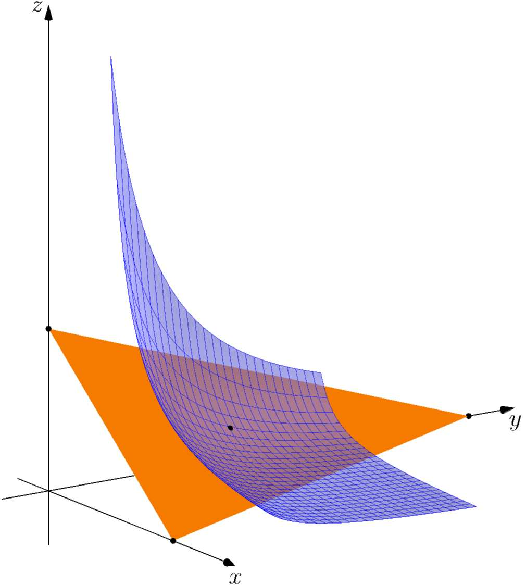
\includegraphics[width=\linewidth]{generated/asymptote/ex4-3.pdf}
\end{image}%
\tcblower
\end{figureptx}%
%
\end{divisionexercise}%
\begin{divisionexercise}{5}{}{}{exercise-supptdir-5}%
Ache a reta tangente à intersecção do gráfico da função \(f(x,y) = x^3+y^3+2\) com o cilindro \(x^2+y^2=2\) no ponto \((1,1,4)\).%
\par\smallskip%
\noindent\textbf{\blocktitlefont Dica}.\hypertarget{hint-supptdir-5-b}{}\quad{}Reconheça as superfícies dadas como superfícies de nível de duas funções de três variáveis.%
\par\smallskip%
\noindent\textbf{\blocktitlefont Resposta}.\hypertarget{answer-supptdir-5-c}{}\quad{}A reta desejada tem equação \(r\colon (x,y,z) = (1,1,4) +
\lambda (1,-1,0)\), \(\lambda \in \mathbb{R}\).%
\par\smallskip%
\noindent\textbf{\blocktitlefont Solução}.\hypertarget{solution-supptdir-5-d}{}\quad{}Seguindo o resultado da \hyperref[proposition-prop_intsupniv]{Proposição~{\xreffont\ref{proposition-prop_intsupniv}}}, consideremos as funções de classe \(\mathscr{C}^1\) dadas por%
\begin{equation*}
F(x,y,z) = x^3 + y^3 +2 - z \quad \text{e} \quad G(x,y,z) =
x^2 + y^2.
\end{equation*}
O gráfico de \(f\) e o cilindro dado são, respectivamente, a superfície de nível \(c=0\) de \(F\) e a superfície de nível \(c=2\) de \(G\). Como os vetores%
\begin{equation*}
\nabla F(1,1,4) = (3,3, -1) \quad \text{e} \quad \nabla
G(1,1,4) = (2,2,0)
\end{equation*}
são linearmente independentes, sabemos que a reta pedida é a única reta que passa pelo ponto \((1,1,4)\) e tem o vetor%
\begin{equation*}
\vec{v}=\nabla F(1,1,4) \times
\nabla G(1,1,4) = (1,-1,0)
\end{equation*}
como vetor diretor. Sua equação é, portanto,%
\begin{equation*}
r\colon (x,y,z) = (1,1,4) + \lambda (1,-1,0),
\lambda \in \mathbb{R}.
\end{equation*}
\begin{figureptx}{Figura}{As superfícies de nível e sua interseção no ponto dado.}{figure-fig_ex4-5}{}%
\begin{image}{0.25}{0.5}{0.25}{}%
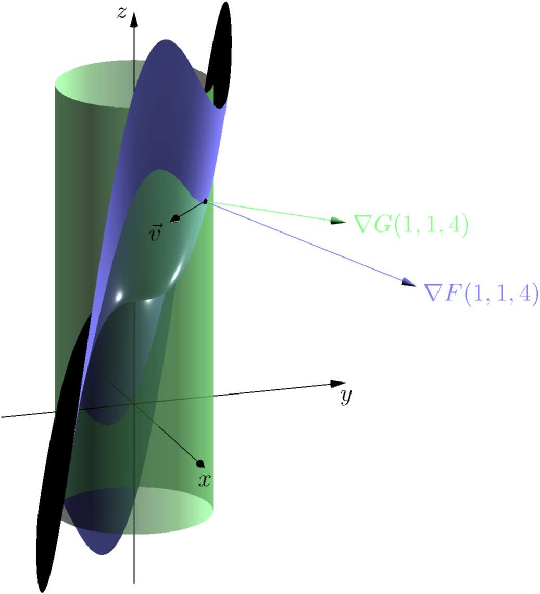
\includegraphics[width=\linewidth]{generated/asymptote/ex4-5.pdf}
\end{image}%
\tcblower
\end{figureptx}%
%
\end{divisionexercise}%
\begin{divisionexercise}{7}{}{}{exercise-supptdir-7}%
Determine a equação da esfera que tangencia a superfície \((x-1)^2 + \dfrac{(y-2)^2}{4} - (z-1)^2 =0\) nos pontos \((2,2,2)\) e \((2,2,0)\).%
\par\smallskip%
\noindent\textbf{\blocktitlefont Dica}.\hypertarget{hint-supptdir-7-b}{}\quad{}Escreva a equação de uma esfera arbitrária em \(\R^3\) e use as condições do enunciado para determinar seu centro e seu raio.%
\par\smallskip%
\noindent\textbf{\blocktitlefont Resposta}.\hypertarget{answer-supptdir-7-c}{}\quad{}A esfera desejada tem equação \((x-3)^2 + (y-2)^2 + (z-1)^2
= 2\).%
\par\smallskip%
\noindent\textbf{\blocktitlefont Solução}.\hypertarget{solution-supptdir-7-d}{}\quad{}Nosso objetivo é determinar \((x_0,y_0,z_0) \in \R^3\) (centro) e \(R>0\) (raio) de modo que a esfera de equação \((x-x_0)^2 + (y-y_0)^2 + (z-z_0)^2 = R^2\) tangencie o cone \((x-1)^2 + \dfrac{(y-2)^2}{4} - (z-1)^2 =0\) nos pontos \((2,2,2)\) e \((2,2,0)\). Isto significa que esta esfera deve passar pelos pontos \((2,2,2)\) e \((2,2,0)\) e, além disso, seus planos tangentes nestes pontos devem coincidir com os respectivos planos tangentes do cone. Vamos considerar, em vista da \hyperref[proposition-prop_supniv]{Proposição~{\xreffont\ref{proposition-prop_supniv}}}, as funções de classe \(\mathscr{C}^1\) dadas por%
\begin{align*}
F(x,y,z)& = (x-x_0)^2 + (y-y_0)^2 + (z-z_0)^2\quad\text{e}\\
G(x,y,z)& = (x-1)^2 + \frac{(y-2)^2}{4} -
(z-1)^2.
\end{align*}
%
\par
A esfera procurada e o cone dado são, respectivamente, a superfície de nível \(c=R^2\) de \(F\) e a superfície de nível \(c=0\) de \(G\). Lembrando que os gradientes são normais às superfícies de nível, queremos%
\begin{align*}
\nabla F(2,2,2) \parallel\nabla G(2,2,2) &\implies
(4-2x_0, 4-2y_0, 4-2z_0) \parallel (2,0,-2)\\
&\implies \begin{cases} 2-x_0 = z_0-2\\ 2-y_0=0
\end{cases} \implies \begin{cases} z_0 = 4-x_0\\ y_0=2,
\end{cases}
\end{align*}
bem como%
\begin{align*}
\nabla F(2,2,0)\parallel \nabla G(2,2,0) &\implies
(4-2x_0, 4-2y_0, -2z_0)\parallel (2,0,2)\\
&\implies \begin{cases} 2-x_0 = -z_0\\2-y_0=2
\end{cases} \implies \begin{cases} z_0 = x_0 - 2\\ y_0=2
\end{cases}
\end{align*}
de modo que \(x_0 = 3\), \(y_0 = 2\) e \(z_0=1\). Para encontrar o raio, basta usarmos que os pontos \((2,2,2)\) e \((2,2,0)\) devem pertenver à esfera:%
\begin{equation*}
(2-3)^2 + (2-2)^2 +
(2-1)^2 = R^2 = (2-3)^2 + (2-2)^2 + (0-1)^2\implies R =
\sqrt{2}.
\end{equation*}
Logo, a esfera procurada tem equação \((x-3)^2 +
(y-2)^2 + (z-1)^2 = 2\). \begin{figureptx}{Figura}{As superfícies de nível e os pontos de tangência.}{figure-fig_ex4-7}{}%
\begin{image}{0.25}{0.5}{0.25}{}%
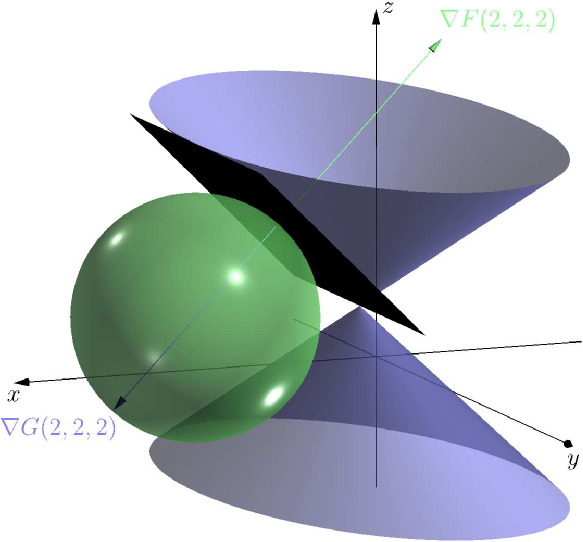
\includegraphics[width=\linewidth]{generated/asymptote/ex4-7.pdf}
\end{image}%
\tcblower
\end{figureptx}%
%
\par
Representamos os gradientes e o plano tangente compartilhado apenas no ponto \((2,2,2)\) para evitar poluição visual na figura acima.%
\end{divisionexercise}%
\end{exercises-subsection-numberless}
\end{sectionptx}
%
%
\typeout{************************************************}
\typeout{Seção 1.10 Classificação de pontos críticos em abertos de \(\R^2\)}
\typeout{************************************************}
%
\begin{sectionptx}{Seção}{Classificação de pontos críticos em abertos de \(\R^2\)}{}{Classificação de pontos críticos em abertos de \(\R^2\)}{}{}{section-sec_maxminloc}
%
%
\typeout{************************************************}
\typeout{Exercícios 1.10 Exercícios}
\typeout{************************************************}
%
\begin{exercises-subsection-numberless}{Exercícios}{Exercícios}{}{Exercícios}{}{}{exercises-ex_maxminloc}
\begin{divisionexercise}{2}{}{}{exercise-maxminloc-2}%
Determine os valores de \(a\) para os quais a função \(f(x,y) = 2ax^4 + y^2 -ax^2 - 2y\)%
\begin{enumerate}[label=\alph*.]
\item{}tenha exatamente um ponto de sela e dois pontos de mínimo local;%
\item{}tenha exatamente dois pontos de sela e um ponto de mínimo local.%
\item{}Existe \(a\in\R\) para o qual \(f\) tenha ao menos um ponto de máximo local?%
\item{}Existe \(a\in\R\) para o qual \(f\) tenha mais de \(3\) pontos críticos?%
\end{enumerate}
%
\par\smallskip%
\noindent\textbf{\blocktitlefont Dica}.\hypertarget{hint-maxminloc-2-b}{}\quad{}Para todos os itens, encontre os pontos críticos de \(f\) e classifique-os usando o Critério da Hessiana. Convém separar os casos \(a>0\), \(a<0\) e \(a=0\).%
\par\smallskip%
\noindent\textbf{\blocktitlefont Resposta}.\hypertarget{answer-maxminloc-2-c}{}\quad{}%
\begin{enumerate}[label=\alph*.]
\item{}\(\displaystyle a>0\)%
\item{}\(\displaystyle a<0\)%
\item{}Não existe valor de \(a\) para o qual \(f\) tenha ao menos um ponto de máximo local.%
\item{}Sim, apenas \(a=0\).%
\end{enumerate}
%
\par\smallskip%
\noindent\textbf{\blocktitlefont Solução}.\hypertarget{solution-maxminloc-2-d}{}\quad{}O gradiente de \(f\) é \(\nabla(x,y) = (8ax^3 -2ax,
2y-2)\). Deste modo,%
\begin{equation*}
\nabla(x,y) = (0,0) \iff
\begin{cases} ax(4x^2-1)=0\\ y=1 \end{cases} \iff \begin{cases}
a=0 \text{ ou } x=0\text{ ou }x= \pm \dfrac{1}{2} \\ y=1 \end{cases}.
\end{equation*}
Assim, se \(a\neq 0\), os únicos pontos críticos de \(f\) são \((0,1)\) e \(\Big(\pm \dfrac{1}{2}, 1\Big)\). Por outro lado, se \(a=0\), então os pontos críticos de \(f\) são todos os pontos da forma \((x,1)\) com \(x \in \R\). Para classificá-los, dividiremos a análise em três casos. Observamos que as derivadas de segunda ordem de \(f\) são%
\begin{equation*}
\frac{\partial^2 f}{\partial x^2}(x,y) = 24a x^2 -2a, \quad
\frac{\partial^2 f}{\partial y \partial x}(x,y) = 0 \quad
\text{e} \quad \frac{\partial^2 f}{\partial y^2} (x,y) = 2.
\end{equation*}
%
\par
Se \(a>0\), usando o critério do Hessiano (\hyperref[theorem-teo_hess]{Teorema~{\xreffont\ref{theorem-teo_hess}}}), temos%
\begin{itemize}[label=\textbullet]
\item{}\(\det H_f(0,1) = \det\begin{bmatrix}
-2a & 0\\
0 & 2
\end{bmatrix} = -4a < 0 \implies (0,1)\) é ponto de sela de \(f\).%
\item{}\(\det H_f\Big(\pm\dfrac{1}{2},1\Big) = \det\begin{bmatrix}
4a & 0\\
0 & 2
\end{bmatrix} = 8a > 0\) e \(8a>0 \implies
\Big(\pm\dfrac{1}{2},1\Big)\) são pontos de mínimo locais \(f\).%
\end{itemize}
%
\par
Se \(a<0\), usamos novamente o critério do Hessiano:%
\begin{itemize}[label=\textbullet]
\item{}\(\det H_f(0,1) =\det \begin{bmatrix}
-2a & 0\\
0 & 2
\end{bmatrix} = -4a > 0\) e \(-2a>0 \implies
(0,1)\) é ponto de mínimo local de \(f\).%
\item{}\(\det H_f\Big(\pm\dfrac{1}{2},1\Big) = \det\begin{bmatrix}
4a & 0\\
0 & 2
\end{bmatrix} = 8a < 0 \implies \Big(\pm\dfrac{1}{2},1\Big)\) são pontos de sela de \(f\).%
\end{itemize}
%
\par
Finalmente, se  \(a=0\), notamos que \(f(x,y)=y^2 - 2y =
(y-1)^2 -1 \geq -1\) para todo \((x,y) \in \R^2\). Como \(f(x,1) = -1\) para todo \(x\in\R\), todos os pontos críticos de \(f\) são pontos de mínimo (globais) neste caso.%
\par
Com a análise acima, estamos em condições de responder cada item do enunciado:%
\begin{enumerate}[label=\alph*.]
\item{}\(f\) terá exatamente um ponto de sela e dois pontos de mínimo local se, e somente se, \(a>0\).%
\item{}\(f\) terá exatamente um ponto de mínimo local e dois pontos de sela se, e somente se, \(a<0\).%
\item{}Não existe valor de \(a\) para o qual \(f\) tenha ao menos um ponto de máximo local.%
\item{}\(f\) terá mais de \(3\) pontos críticos se, e somente se, \(a=0\).%
\end{enumerate}
%
\begin{figureptx}{Figura}{Gráfico de \(f\), com \(a>0\).}{figure-fig_exmaxminlocapos}{}%
\begin{image}{0.25}{0.5}{0.25}{}%
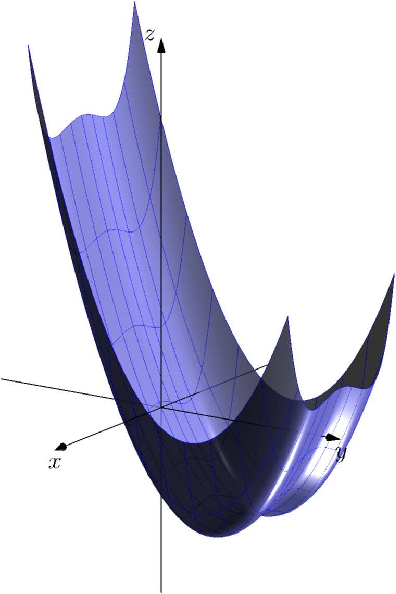
\includegraphics[width=\linewidth]{generated/asymptote/exmaxminlocapos.pdf}
\end{image}%
\tcblower
\end{figureptx}%
\begin{figureptx}{Figura}{Gráfico de \(f\), com \(a<0\).}{figure-maxminloc-2-d-g}{}%
\begin{image}{0.25}{0.5}{0.25}{}%
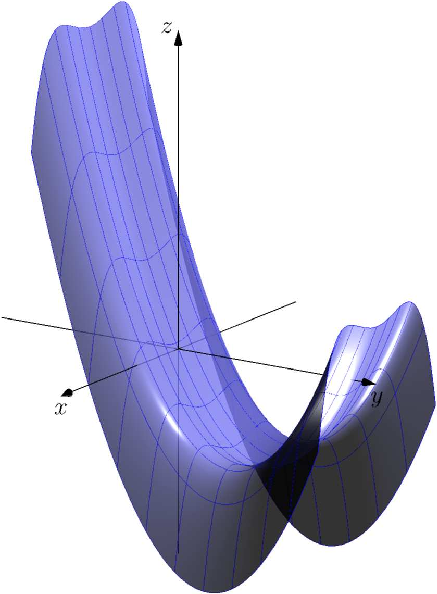
\includegraphics[width=\linewidth]{generated/asymptote/exmaxminlocaneg.pdf}
\end{image}%
\tcblower
\end{figureptx}%
\begin{figureptx}{Figura}{Gráfico de \(f\), com \(a=0\).}{figure-fig_exmaxminlocanul}{}%
\begin{image}{0.25}{0.5}{0.25}{}%
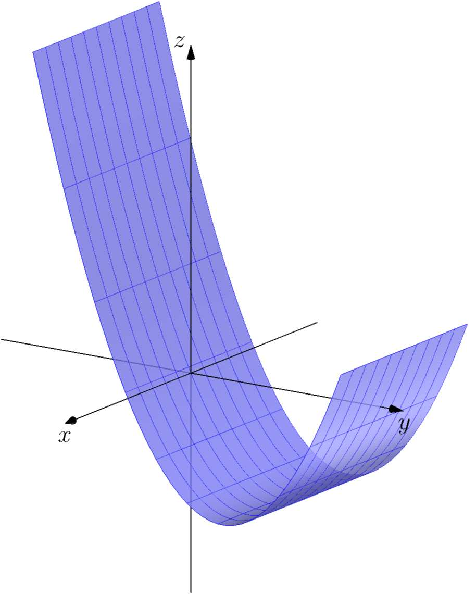
\includegraphics[width=\linewidth]{generated/asymptote/exmaxminlocanul.pdf}
\end{image}%
\tcblower
\end{figureptx}%
\end{divisionexercise}%
\end{exercises-subsection-numberless}
\end{sectionptx}
%
%
\typeout{************************************************}
\typeout{Seção 1.11 Máximos e mínimos em conjuntos compactos}
\typeout{************************************************}
%
\begin{sectionptx}{Seção}{Máximos e mínimos em conjuntos compactos}{}{Máximos e mínimos em conjuntos compactos}{}{}{section-sec_maxmincpt}
%
%
\typeout{************************************************}
\typeout{Exercícios 1.11 Exercícios}
\typeout{************************************************}
%
\begin{exercises-subsection-numberless}{Exercícios}{Exercícios}{}{Exercícios}{}{}{exercises-ex_maxmincpt}
\begin{divisionexercise}{3.b}{}{}{exercise-maxmincpt-3b}%
Determine o valor máximo e o valor mínimo de \(f(x,y,z) =
x^2 + y^2 +2z^2 -4xy -4z + 3x\) na região \(R = \big\{(x,y,z)
\in \R^3\colon x+y+z \leq 4, x\geq 0, y\geq 0\text{ e }
z\geq0\big\}\).%
\par\smallskip%
\noindent\textbf{\blocktitlefont Dica}.\hypertarget{hint-maxmincpt-3b-b}{}\quad{}Divida a análise em três etapas: no interior de \(R\), nas faces de \(R\) (excluídas as arestas) e nas arestas (atenção aos vértices!).%
\par\smallskip%
\noindent\textbf{\blocktitlefont Resposta}.\hypertarget{answer-maxmincpt-3b-c}{}\quad{}O valor máximo de \(f\) é \(28\) e o valor mínimo de \(f\) é \(-\dfrac{11}{4}\).%
\par\smallskip%
\noindent\textbf{\blocktitlefont Solução}.\hypertarget{solution-maxmincpt-3b-d}{}\quad{}Note que \(f\) é contínua e \(R\) é um tetraedro sólido, fechado e limitado, portanto compacto. Deste modo o Teorema de Weierstrass (\hyperref[theorem-teo_wei]{Teorema~{\xreffont\ref{theorem-teo_wei}}}) assegura que o problema proposto tem solução.%
\par
A análise será dividida em três etapas: encontraremos os candidatos no interior de \(R\), no "interior" das faces de \(R\) (isto é, as faces com as arestas excluídas) e, finalmente, nas arestas de \(R\). O motivo dessa análise "excluindo" essas "fronteiras", fica claro ao estudar a demonstração dos teoremas finais da \hyperref[section-ap_maxmincond]{Seção~{\xreffont\ref{section-ap_maxmincond}}} (\hyperref[theorem-teo_lag31]{Teorema~{\xreffont\ref{theorem-teo_lag31}}} e \hyperref[theorem-teo_lag32]{Teorema~{\xreffont\ref{theorem-teo_lag32}}}).%
\par
Ao trabalho:%
\begin{itemize}[label=\textbullet]
\item{}Candidatos no interior de \(R\): o interior de \(R\) é o conjunto (aberto)%
\begin{equation*}
\text{int}(R) = \big\{(x,y,z) \in
\R^3\colon x+y+z < 4, x> 0, y> 0\text{ e } z>
0\big\}.
\end{equation*}
Neste caso, usamos a versão para três variáveis (totalmente análoga) do \hyperref[theorem-teo_crit]{Teorema~{\xreffont\ref{theorem-teo_crit}}}, concluindo que os candidatos são os pontos críticos de \(f\) neste conjunto. Como%
\begin{equation*}
\nabla f(x,y,z) = (2x-4y+3, 2y-4x,
4z-4),
\end{equation*}
o único ponto crítico é \(\big(\dfrac{1}{2}, 1,
1\big)\). Note que este ponto pertence a int\((R)\).%
\item{}Candidatos nas faces (excluídas as arestas): procuramos os candidatos nos conjuntos%
\begin{align*}
F_1 &= \big\{(x,y,z) \in \R^3\colon x+y+z = 4,
x>0, y>0\text{ e } z>0\big\},\\
F_2 &= \big\{(x,y,z) \in \R^3\colon x+y+z < 4,
x= 0, y> 0\text{ e } z> 0\big\},\\
F_3 &= \big\{(x,y,z) \in \R^3\colon x+y+z < 4,
x> 0, y= 0\text{ e } z> 0\big\},\\
F_4 &= \big\{(x,y,z) \in \R^3\colon x+y+z < 4,
x> 0, y> 0\text{ e } z= 0\big\}.
\end{align*}
São as faces de \(R\), excluídas as arestas. Em cada face, vamos "eliminar" uma das variáveis e reduzir o problema ao estudo de funções de duas variáveis em abertos de \(\R^2\). Outra abordagem possível seria usar o Método dos Multiplicadores de Lagrange (\hyperref[theorem-teo_lag31]{Teorema~{\xreffont\ref{theorem-teo_lag31}}}), o qual foi utilizado no \hyperlink{exercise-maxminarb-5}{Exercício~{\xreffont 1.12.5}}.%
\par
Na face \(F_1\), podemos escrever \(z = 4 - x - y\) e estudar a função%
\begin{equation*}
g_1(x,y) = f(x,y,4-x-y) = 3x^2 + 3y^2 -9x
-12y +16
\end{equation*}
no aberto%
\begin{equation*}
U_1 = \big\{ (x,y) \in \R^2\colon
x+ y<4, x >0\text{ e } y>0\big\}.
\end{equation*}
Como%
\begin{equation*}
\nabla g_1(x,y) = (6x-9, 6y-12),
\end{equation*}
o ponto \(\Big(
\dfrac{3}{2}, 2\Big) \in U_1\) é o único ponto crítico de \(g_1\). Este ponto corresponde ao candidato \(\Big(
\dfrac{3}{2}, 2, \dfrac{1}{2}\Big) \in F_1\).%
\par
Na face \(F_2\), temos \(x=0\) e estudamos a função%
\begin{equation*}
g_2(y,z) = f(0,y,z) = y^2 + 2z^2 -4z
\end{equation*}
no aberto%
\begin{equation*}
U_2 = \big\{ (y,z) \in \R^2\colon y+z < 4, y >
0\text{ e } z>0\big\}.
\end{equation*}
Como%
\begin{equation*}
\nabla g_2(y,z) =
(2y,4z-4),
\end{equation*}
o único ponto crítico de \(g_2\) é \((0,1)\), que \emph{não} pertence a \(U_2\). Deste modo, não há candidatos em \(F_2\).%
\par
Em \(F_3\), obtemos a função%
\begin{equation*}
g_3(x,z) = f(x,0,z) =
x^2 + 2z^2 -4z + 3x
\end{equation*}
no aberto%
\begin{equation*}
U_3 = \big\{ (x,z) \in
\R^2\colon x+z < 4, x > 0\text{ e } z>0\big\}.
\end{equation*}
O gradiente de \(g_3\)%
\begin{equation*}
\nabla g_3(x,z) = (2x+3,4z-4)
\end{equation*}
se anula apenas no ponto \(\Big( -\dfrac{3}{2}, 1\Big)\), que \emph{não} pertence a \(U_3\). Também não temos candidatos em \(F_3\).%
\par
Finalmente, em \(F_4\), analisamos%
\begin{equation*}
g_4(x,y)=f(x,y,0)
= x^2 + y^2 -4xy+3x
\end{equation*}
no aberto%
\begin{equation*}
U_4 =
\big\{(x,y)\in\R^2\colon x+y < 4, x>0\text{ e }y>
0\big\}=U_1.
\end{equation*}
Como%
\begin{equation*}
\nabla g_4(x,y) = (2x-4y+3,
2y-4x),
\end{equation*}
o único ponto crítico de \(g_4\) é o ponto \(\Big(\dfrac{1}{2},1\Big) \in U_4\), que corresponde ao candidato \(\Big( \dfrac{1}{2}, 1, 0\Big) \in F_4\).%
\par
Isto completa a busca dos candidatos nas faces de \(R\).%
\item{}Candidatos nas arestas de \(R\): as arestas de \(R\) são os segmentos de reta%
\begin{align*}
A_1 &= \big\{(x,y,z) \in \R^3\colon y=z=0\text{ e }
0 \leq x \leq 4\big\},\\
A_2 &= \big\{(x,y,z) \in \R^3\colon x=z=0\text{ e }
0 \leq y \leq 4\big\},\\
A_3 &= \big\{(x,y,z) \in \R^3\colon x=y=0\text{ e }
0 \leq z \leq 4\big\},\\
A_4 &= \{(x,y,z) \in \R^3\colon z=0\text{ e }
x+y=4\big\},\\
A_5 &= \{(x,y,z) \in \R^3\colon y=0\text{ e }
x+z=4\big\},\\
A_6 &= \{(x,y,z) \in \R^3\colon x=0\text{ e }
y+z=4\big\}.
\end{align*}
A estratégia é parametrizar cada aresta a estudar a composta de \(f\) com as parametrizações. Poderíamos aqui aplicar o Método dos Multiplicadores de Lagrange (\hyperref[theorem-teo_lag32]{Teorema~{\xreffont\ref{theorem-teo_lag32}}}), como fizemos no \hyperlink{exercise-maxmincpt-4b}{Exercício~{\xreffont 1.11.4.b}}.%
\par
Em \(A_1\), consideramos%
\begin{equation*}
h_1(x) = f(x,0,0) = x^2 + 3x, x \in [0,4].
\end{equation*}
A derivada de \(h_1\) se anula somente em \(x=-\frac{3}{2}\), de modo que não há candidatos em \(]0,4[\). Ficamos apenas com \(x=0\) e \(x=4\), que correspondem aos vértices \((0,0,0)\) e \((4,0,0)\) de \(R\).%
\par
Em \(A_2\), estudamos%
\begin{equation*}
h_2(y) = f(0,y,0) = y^2, y \in [0,4].
\end{equation*}
Como \(h_2\) é estritamente crescente, os candidatos são \(y=0\) e \(y=4\), que correspondem aos vértices \((0,0,0)\) e \((0,4,0)\).%
\par
Em \(A_3\), obtemos%
\begin{equation*}
h_3(z) = 2z^2 -4z, z \in
[0,4],
\end{equation*}
cuja derivada se anula em \(z=1\). Os candidatos são \(z=0\), \(z=1\) e \(z=4\), que correspondem, respectivamente, a \((0,0,0)\), \((0,0,1)\) e \((0,0,4)\).%
\par
Em \(A_4\), podemos escrever \(y=4-x\) para obter%
\begin{equation*}
h_4(x) = f(x,4-x,0) = 6x^2 -21x + 16, x \in [0,4].
\end{equation*}
O único ponto crítico de \(h_4\) é \(x=\dfrac{7}{4} \in
]0,4[\). Os candidatos são \(x=0\), \(x= \dfrac{7}{4}\) e \(x=4\), que correspondem a \((0,4,0)\), \(\Big(\dfrac{7}{4}, \dfrac{9}{4}, 0\Big)\) e \((4, 0,
0)\).%
\par
Em \(A_5\), fazemos \(z=4-x\) e estudamos%
\begin{equation*}
h_5(x) =
f(x,0,4-x) = 3x^2 -9x+16, x \in [0,4].
\end{equation*}
O único ponto crítico de \(h_5\) é \(x=\dfrac{3}{2} \in ]0,4[\). Os candidatos são \(x=0\), \(x= \dfrac{3}{2}\) e \(x=4\), que correspondem a \((0,0,4)\), \(\Big( \dfrac{3}{2},0,
\dfrac{5}{2}\Big)(4, 0, 0)\).%
\par
Finalmente, em \(A_6\), escrevemos \(z=4-y\) e%
\begin{equation*}
h_6(y) = f(0,y,4-y) = 3y^2 -12y+16, y \in [0,4].
\end{equation*}
O único ponto crítico de \(h_6\) é \(y=2\in ]0,4[\). Os candidatos são \(y=0\), \(y= 2\) e \(y=4\), que correspondem a \((0,0,4)\), \((0, 2,2)\) e \((0, 4, 0)\).%
\item{}Avaliando \(f\) em cada candidato: só resta calcular \(f\) nos pontos encontrados nas etapas anteriores e comparar os valores. Confira as contas!%
\begin{align*}
f( 1/2, 1, 1) &= -5/4\\
f( {3}/{2}, 2,{1}/{2}) &= -{11}/{4}\\
f( {1}/{2}, 1, 0) &= {3}/{4}\\
f\left( 0,0,0\right) &= 0\\
f\left(4, 0, 0\right) &= 28\\
f\left( 0,4,0\right) &= 16\\
f\left( 0,0,4 \right) &= 16\\
f\left( 0, 0, 1\right) &= -2\\
f\left( {7}/{4}, {9}/{4}, 0\right) &= -{19}/{8}\\
f\left( {3}/{2}, 0, {5}/{2}\right) &= {37}/{4}\\
f\left( 0, 2, 2\right) &= 4
\end{align*}
%
\end{itemize}
Logo, o maior valor de \(f\) em \(R\) é \(28\) e o menor valor é \(-\frac{11}{4}\).%
%
\end{divisionexercise}%
\begin{divisionexercise}{4.b}{}{}{exercise-maxmincpt-4b}%
Encontre os pontos de máximo e de mínimo de \(f(x,y,z) =
x-z\) em \(C = \big\{(x,y,z) \in \R^3\colon x^2 + y^2 =z
\text{ e } z=2y\big\}\), sem parametrizar o conjunto \(C\). Repita o exercício parametrizando \(C\).%
\par\smallskip%
\noindent\textbf{\blocktitlefont Dica}.\hypertarget{hint-maxmincpt-4b-b}{}\quad{}Use o Método dos Multiplicadores de Lagrange para resolver sem parametrizar \(C\).%
\par\smallskip%
\noindent\textbf{\blocktitlefont Resposta}.\hypertarget{answer-maxmincpt-4b-c}{}\quad{}O ponto de máximo de \(f\) em \(C\) é \(\big(\dfrac{1}{\sqrt{5}}, 1 - \dfrac{2}{\sqrt{5}}, 2 -
\dfrac{4}{\sqrt{5}}\big)\). O ponto de mínimo de \(f\) em \(C\) é \(\big( -\dfrac{1}{\sqrt{5}}, 1 + \dfrac{2}{\sqrt{5}}, 2 +
\dfrac{4}{\sqrt{5}}\big)\).%
\par\smallskip%
\noindent\textbf{\blocktitlefont Solução}.\hypertarget{solution-maxmincpt-4b-d}{}\quad{}Note que \(f\) é contínua e \(C\) é compacto, de modo que o Teorema de Weierstrass (veja \hyperref[theorem-teo_wei]{Teorema~{\xreffont\ref{theorem-teo_wei}}}) assegura que o problema proposto tem solução.%
%
\begin{itemize}[label=\textbullet]
\item{}Primeira solução: Usando o Método dos Multiplicadores de Lagrange.%
\par
Nosso objetivo é encontrar os pontos de máximo e mínimo de \(f\) sujeita às condições \(x^2 + y^2 = z\) e \(z=2y\). Consideremos as funções de classe \(\mathscr{C}^1\)%
\begin{equation*}
g(x,y,z) = x^2 + y^2 - z \quad
\text{e}\quad h(x,y,z) = 2y-z.
\end{equation*}
%
\par
O conjunto \(C\) é a intersecção das superfícies de nível \(c=0\) de \(g\) e de \(h\). Observamos primeiramente que os gradientes de \(g\) e \(h\),%
\begin{equation*}
\nabla g(x,y,z) = (2x,2y,-1), \quad
\nabla h(x,y,z) = (0,2,-1),
\end{equation*}
são linearmente independentes em \(C\). De fato, estes vetores são paralelos se, e somente se, \(x=0\) e \(y=1\), e nenhum ponto da forma \((0,1,z)\) pode pertencer a \(C\) (por quê?). Deste modo, o Método dos Multiplicadores de Lagrange garante que os candidatos a pontos de máximo e mínimo de \(f\) são as soluções do sistema%
\begin{equation*}
\begin{cases}
\big\{\nabla f(x,y,z), \nabla g(x,y,z), \nabla
h(x,y,z)\big\}\text{ é linearmente dependente},\\
x^2 + y^2 = z,\\
z=2y.
\end{cases}
\end{equation*}
Como \(\nabla f(x,y,z) = (1,0,-1)\), a primeira condição equivale a%
\begin{equation*}
\det\begin{bmatrix}
1& 0 & -1\\
2x & 2y & -1\\
0 & 2 & -1
\end{bmatrix} = 0 \iff y
= -2x+1.
\end{equation*}
Substituindo esta equação nas outras duas, obtemos \(z=-4x+2\) e \(x = \pm \frac{1}{\sqrt{5}}\). Os candidatos são, portanto, os pontos%
\begin{equation*}
\big( \sfrac{1}{\sqrt{5}}, 1 -
\sfrac{2}{\sqrt{5}}, 2 - \sfrac{4}{\sqrt{5}}\big) \quad
\text{e} \quad \big( -\dfrac{1}{\sqrt{5}}, 1 +
\dfrac{2}{\sqrt{5}}, 2 + \dfrac{4}{\sqrt{5}}\big).
\end{equation*}
Como \(f\big( \dfrac{1}{\sqrt{5}}, 1 - \dfrac{2}{\sqrt{5}}, 2 -
\dfrac{4}{\sqrt{5}}\big) = \sqrt{5}-2\) e \(f\big(
-\dfrac{1}{\sqrt{5}}, 1 + \dfrac{2}{\sqrt{5}}, 2 +
\dfrac{4}{\sqrt{5}}\big) = -\sqrt{5} -2\), tratam-se, respectivamente, do ponto de máximo e do ponto de mínimo de \(f\) em \(C\).%
\item{}Segunda solução: Parametrizando o conjunto \(C\).%
\par
Escrevendo \(z = x^2 + y^2 = 2y\) e completando quadrados, obtemos \(x^2 + (y-1)^2 = 1\). Assim, uma parametrização de \(C\) é \(\gamma\colon [0,2\pi]\to\R^3\) dada por%
\begin{equation*}
\gamma(t) =
(\cos t, \sin t + 1, 2\sin t + 2).
\end{equation*}
%
\par
Desejamos encontrar os pontos de máximo e mínimo da composta%
\begin{equation*}
g(t) = f(\gamma(t)) = \cos t - 2\sin t -2,
\end{equation*}
no intervalo \([0,2\pi]\) (um problema de Cálculo I). Os candidatos são os pontos críticos de \(g\) no intervalo \(]0, 2\pi[\) e os extremos \(t=0, t=2\pi\). Como%
\begin{equation*}
g'(t) = -\sin t -2 \cos t = 0 \iff \sin t = -2 \cos
t,
\end{equation*}
os pontos críticos de \(g\) são as soluções (no intervalo \(]0, 2\pi[\)) da equação%
\begin{equation*}
\cos^2 t = 1 -
\sin^2 t = 1 - 4 \cos^2 t \iff \cos t = \pm
\dfrac{1}{\sqrt{5}}.
\end{equation*}
Para \(\cos t =
\dfrac{1}{\sqrt{5}}\), temos \(\sin t =
-\dfrac{2}{\sqrt{5}}\), que corresponde ao ponto \(\big(
\dfrac{1}{\sqrt{5}}, 1 - \dfrac{2}{\sqrt{5}}, 2 -
\dfrac{4}{\sqrt{5}}\big) \in C\). Analogamente, \(\cos t =
-\dfrac{1}{\sqrt{5}}\) corresponde ao ponto \(\big(
-\dfrac{1}{\sqrt{5}}, 1 + \dfrac{2}{\sqrt{5}}, 2 +
\dfrac{4}{\sqrt{5}}\big) \in C\). O outro candidato é o ponto \(\gamma(0) = \gamma(2\pi) = (1,1,2) \in C\), no qual \(f\) atinge o valor \(-1\).%
\end{itemize}
\end{divisionexercise}%
\end{exercises-subsection-numberless}
\end{sectionptx}
%
%
\typeout{************************************************}
\typeout{Seção 1.12 Máximos e mínimos em conjuntos arbitrários}
\typeout{************************************************}
%
\begin{sectionptx}{Seção}{Máximos e mínimos em conjuntos arbitrários}{}{Máximos e mínimos em conjuntos arbitrários}{}{}{section-sec_maxminarb}
%
%
\typeout{************************************************}
\typeout{Exercícios 1.12 Exercícios}
\typeout{************************************************}
%
\begin{exercises-subsection-numberless}{Exercícios}{Exercícios}{}{Exercícios}{}{}{exercises-ex_maxminarb}
\begin{divisionexercise}{5}{}{}{exercise-maxminarb-5}%
Determine as dimensões do paralelepípedo de volume máximo, com faces paralelas aos planos coordenados, inscrito no elipsoide \(9x^2 + 36y^2 + 4z^2 = 36\). Justifique a existência de solução.%
\par\smallskip%
\noindent\textbf{\blocktitlefont Dica}.\hypertarget{hint-maxminarb-5-b}{}\quad{}Use o Método dos Multiplicadores de Lagrange para estudar a função volume sujeita à condição \(9x^2 + 36y^2 + 4z^2 =
36\).%
\par\smallskip%
\noindent\textbf{\blocktitlefont Resposta}.\hypertarget{answer-maxminarb-5-c}{}\quad{}Os vértices do paralelepípedo procurado são os pontos \(\big( \pm \dfrac{2}{\sqrt{3}}, \pm \dfrac{1}{\sqrt{3}}, \pm
\sqrt{3}\big)\).%
\par\smallskip%
\noindent\textbf{\blocktitlefont Solução}.\hypertarget{solution-maxminarb-5-d}{}\quad{}Considere um paralelepípedo inscrito no elipsoide \(9x^2 +
36y^2 + 4z^2 = 36\) com faces paralelas aos planos coordenados. Se \((x,y,z)\) é o vértice pertencente ao primeiro octante, então as dimensões do paralelepípedo são \(2x\), \(2y\) e \(2z\), de modo que seu volume é igual a%
\begin{equation*}
V(x,y,z) = 8xyz.
\end{equation*}
Isto sugere estudar a função \(V\) sujeita à condição \(9x^2 + 36y^2 + 4z^2 =
36\). Vamos usar o Método dos Multiplicadores de Lagrange (\hyperref[theorem-teo_lag31]{Teorema~{\xreffont\ref{theorem-teo_lag31}}}) e, depois, mostrar que o resultado obtido é, de fato, solução do problema. Observamos apenas que \(V\) é contínua e o elipsoide é compacto; de acordo com o Teorema de Weierstrass (\hyperref[theorem-teo_wei]{Teorema~{\xreffont\ref{theorem-teo_wei}}}), \(V\) possui máximo e mínimo neste elipsoide.%
\par
Escrevendo \(g(x,y,z) = 9x^2 + 36y^2 + 4z^2 = 36\), temos%
\begin{equation*}
\nabla g(x,y,z) = 2(9x,36y,4z),
\end{equation*}
que se anula apenas na origem. Assim, os candidatos a máximos e mínimos de \(V\) são as soluções de%
\begin{equation*}
\begin{cases}
\big\{\nabla V(x,y,z), \nabla
g(x,y,z)\big\}\text{ é linearmente dependente},\\
9x^2 + 36y^2 +4z^2 = 36.
\end{cases}
\end{equation*}
A primeira condição equivale a%
\begin{align*}
\nabla V(x,y,z) \times \nabla g(x&,y,z) = (0,0,0)\\
&\iff
(4x(z^2 - 9y^2), y(9x^2 - 4z^2), 9z(4y^2 -x^2)) =
(0,0,0)\\
&\iff \begin{cases}
x=0\text{ ou }z=\pm 3y,\\
y=0\text{ ou }3x=\pm 2z,\\
z=0\text{ ou }x=\pm2 y.
\end{cases}
\end{align*}
%
\par
Nas soluções \((x,y,z)\) do sistema acima com pelo menos uma das coordendas nulas temos \(V(x,y,z)=0\).%
\par
Resta então o caso em que \(z=\pm 3y\) e \(3x=\pm 2z\), com \(xyz\neq 0\). Substituindo estas equações em \(9x^2 +
36y^2 + 4z^2 = 36\), obtemos \(108y^2 = 36\), de modo que \(y=\pm \frac{1}{\sqrt{3}}\). Os candidatos são os (oito) pontos \(\Big(\pm \dfrac{2}{\sqrt{3}}, \pm \dfrac{1}{\sqrt{3}},
\pm\sqrt{3}\Big)\), onde \(V\) vale \(\dfrac{16}{\sqrt{3}}\) ou \(-\dfrac{16}{\sqrt{3}}\), de acordo com os sinais das coordenadas.%
\par
Para verificar que os pontos \(\Big( \pm
\dfrac{2}{\sqrt{3}}, \pm \dfrac{1}{\sqrt{3}}, \pm
\sqrt{3}\Big)\) são os vértices do paralelepípedo de volume máximo satisfazendo as condições do enunciado, basta notar que a função contínua \(|V|\) atinge seu valor máximo precisamente nestes pontos.%
\end{divisionexercise}%
\end{exercises-subsection-numberless}
\end{sectionptx}
\end{chapterptx}
%
%
\typeout{************************************************}
\typeout{Capítulo 2 Provas de 2023}
\typeout{************************************************}
%
\begin{chapterptx}{Capítulo}{Provas de 2023}{}{Provas de 2023}{}{}{chapter-ch_2023}
\renewcommand*{\chaptername}{Capítulo}
\begin{introduction}{}%
Neste capítulo apresentamos as soluções dos exercícios das provas aplicadas em 2023, quando a Escola Politécnica retornou ao calendário com três provas.%
\par
A primeira prova aborda curvas no plan e os conceitos de limite e continuidade de funções a duas variáveis reais.%
\end{introduction}%
%
%
\typeout{************************************************}
\typeout{Seção 2.1 Primeira Prova}
\typeout{************************************************}
%
\begin{sectionptx}{Seção}{Primeira Prova}{}{Primeira Prova}{}{}{section-sec_2023-p1}
%
%
\typeout{************************************************}
\typeout{Exercícios 2.1 Exercícios}
\typeout{************************************************}
%
\begin{exercises-subsection-numberless}{Exercícios}{Exercícios}{}{Exercícios}{}{}{exercises-gab_2023-p1}
\begin{divisionexercise}{1}{}{}{exercise-p1q1-2023}%
Considere a função \(f(x,y)=\dfrac{2x^2-2y^2-1}{x^2+y^2-1}\).%
\begin{enumerate}[label=\alph*]
\item{}Determine o domínio de \(f\), e faça seu esboço com linhas tracejadas, no plano cartesiano abaixo, os pontos que não pertencem a este domínio.%
\item{}Determine as curvas de nível \(c=0\) e \(c=1\), esboçando-as também no plano cartesiano abaixo.%
\item{}Decida, justificando, a existência de \(\lim\limits_{(x,y)\to (\sqrt{3}/2,1/2)}
f(x,y)\).%
\end{enumerate}
\begin{figureptx}{Figura}{Espaço para os esboços pedidos.}{figure-fig_gabp1q1a-2023}{}%
\begin{image}{0.25}{0.5}{0.25}{}%
\resizebox{\linewidth}{!}{%
\begin{tikzpicture}[scale=1]
\draw[help lines,line width=0.1pt,lightgray] (-3.4, -3.4) grid
(3.4, 3.4);
\draw[->] (-3.5,0)--(3.5,0) node[below]{$x$};
\draw[->] (0,-3.5)--(0,3.5) node[right]{$y$};
\end{tikzpicture}
}%
\end{image}%
\tcblower
\end{figureptx}%
%
\par\smallskip%
\noindent\textbf{\blocktitlefont Resposta}.\hypertarget{answer-p1q1-2023-b}{}\quad{}%
\begin{enumerate}[label=\alph*]
\item{}\(\mathrm{Dom} f=\big\{(x,y)\in\R^2\colon x^2+y^2\neq 1\big\}\).%
\item{}Veja na solução.%
\item{}O limite pedido não existe.%
\end{enumerate}
%
\par\smallskip%
\noindent\textbf{\blocktitlefont Solução}.\hypertarget{solution-p1q1-2023-c}{}\quad{}%
\begin{enumerate}[label=\alph*]
\item{}A expressão de \(f\) está definida para todo \((x,y)\in\R^2\), tal que \(x^2+y^2\neq 1\). Em símbolos,%
\begin{equation*}
\mathrm{Dom} f=\big\{(x,y)\in\R^2\colon x^2+y^2\neq
1\big\}.
\end{equation*}
A região a ser excluída no domínio de \(f\) é a circunferência de raio 1 e centro na origem. Veja na figura abaixo.%
\item{}Usando a \hyperref[definition-curva_nivel]{Definição~{\xreffont\ref{definition-curva_nivel}}}, escrevemos as curvas de nível (lembrando que em cada equação devemos ter \(x^2+y^2\neq 1\)):%
\begin{align*}
f^{-1}(0)\colon f(x,y)=0&\iff
2x^2-2y^2-1=0\\
&\iff (\sqrt{2}x)^2-(\sqrt{2}y)^2=1;\\
f^{-1}(1)\colon f(x,y)=1&\iff
2x^2-2y^2-1=x^2+y^2-1\\
&\iff x^2-3y^2=0,
\end{align*}
que são, respectivamente, parte de uma hipérbole com focos no eixo \(Ox\) e parte de um par de retas concorrentes na origem (esboçadas abaixo).%
\par
Observamos que na outra versão da provas as curvas de nível pedidas são parte de uma elipse e parte de um par de retas paralelas (também indicadas na figura).%
\item{}Em vista das duas curvas de nível acima se aproximarem arbitrariamente do ponto \((\frac{\sqrt{3}}{2},\frac{1}{2})\), temos que ao longo de cada uma dessas curvas a função \(f\) tende ao valor do nível da curva (na verdade é constante igual a esse nível em cada curv).%
\par
Isso mostra que \(\lim\limits_{(x,y)\to (\sqrt{3}/2,1/2)}
f(x,y)\) não existe.%
\end{enumerate}
Aqui estão os esboços pedidos: \begin{figureptx}{Figura}{Restrições do domínio e curvas de nível pedidas.}{figure-fig_gabp1q1b-2023}{}%
\begin{image}{0.25}{0.5}{0.25}{}%
\resizebox{\linewidth}{!}{%
\begin{tikzpicture}[scale=1]
\draw[help lines,line width=0.1pt,lightgray] (-3.4, -3.4) grid
(3.4, 3.4);
\draw[->] (-3.5,0)--(3.5,0) node[below]{$x$};
\draw[->] (0,-3.5)--(0,3.5) node[right]{$y$};

\draw[dashed] (0,0) circle (1);

\draw[blue] (-3,{-sqrt(3)})--(3,{sqrt(3)})
node[right]{$c=1$};
\draw[blue] (-3,{sqrt(3)})--(3,{-sqrt(3)});

\draw[olive, domain=-2*pi/5:2*pi/5]
plot({1/sqrt(2)*sec(\x r)},{1/sqrt(2)*tan(\x r)})
node[right]{$c=0$};
\draw[olive, domain=-2*pi/5:2*pi/5]
plot({-1/sqrt(2)*sec(\x r)},{1/sqrt(2)*tan(\x r)});

\draw[red] (-3,1/2)--(3,1/2) node[right]{$c=2$};
\draw[red] (-3,-1/2)--(3,-1/2);

\draw[orange] (0,0) ellipse ({sqrt(2)} and {sqrt(2/5)})
node[right,xshift=40,yshift=5]{$c=3$};

\filldraw[fill=white] ({sqrt(3)/2},1/2) circle (1pt);
\filldraw[fill=white] ({-sqrt(3)/2},1/2) circle (1pt);
\filldraw[fill=white] ({sqrt(3)/2},-1/2) circle (1pt);
\filldraw[fill=white] ({-sqrt(3)/2},-1/2) circle (1pt);

\end{tikzpicture}
}%
\end{image}%
\tcblower
\end{figureptx}%
%
 \par
Por que não um esboço do gráfico da função enfatizando os níveis indicados: \begin{figureptx}{Figura}{Gráfico de função e cortes de nível}{figure-fig_gabp1q1c-2023}{}%
\begin{image}{0.25}{0.5}{0.25}{}%
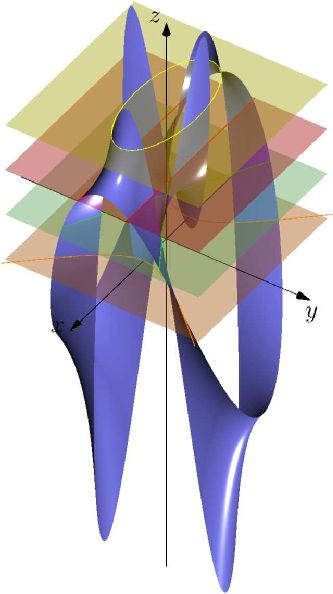
\includegraphics[width=\linewidth]{generated/asymptote/gabp1q1c-2023.pdf}
\end{image}%
\tcblower
\end{figureptx}%
%
%
\end{divisionexercise}%
\begin{divisionexercise}{2}{}{}{exercise-p1q2-2023}%
%
\begin{enumerate}[label=\alph*]
\item{}Calcule ou mostre que não existe:%
\begin{enumerate}[label=\roman*]
\item{}\(\lim\limits_{(x,y)\to
(0,0)}\dfrac{x^2y}{x^4+y^2}e^{-1/(x^4+y^2)}\);%
\item{}\(\lim\limits_{(x,y)\to (1,0)}\dfrac{y^2}{x-1}\).%
\end{enumerate}
%
\item{}Seja \(F(x,y)=
\begin{cases}
\dfrac{\sin x}{y},& \text{ se }y\neq0;\\
\hfill 1,& \text{ se }y=0
\end{cases}\). Decida, justificando, se \(F\) é contínua em \((0,0)\).%
\end{enumerate}
%
\par\smallskip%
\noindent\textbf{\blocktitlefont Resposta}.\hypertarget{answer-p1q2-2023-b}{}\quad{}%
\begin{enumerate}[label=\alph*]
\item{}%
\begin{enumerate}[label=\roman*]
\item{}\(0\);%
\item{}Não existe.%
\end{enumerate}
%
\item{}\(F\) não é contínua em \((0,0)\).%
\end{enumerate}
%
\par\smallskip%
\noindent\textbf{\blocktitlefont Solução}.\hypertarget{solution-p1q2-2023-c}{}\quad{}%
\begin{enumerate}[label=\alph*]
\item{}%
\begin{enumerate}[label=\roman*]
\item{}Temos ao menos duas soluções diferentes aqui:%
\begin{itemize}[label=\textbullet]
\item{}Notamos que \(\dfrac{x^2y}{x^4+y^2}\) é limitada (análogo ao caso de \(\dfrac{xy}{x^2+y^2}\)) e que \(e^{-1/(x^4+y^2)}\)tende a zero, já que \(u=x^4+y^2\) é contínua e tende a zero quando \((x,y)\to (0,0)\) e então%
\begin{equation*}
\lim\limits_{(x,y)\to
(0,0)}e^{-1/(x^4+y^2)}=\lim\limits_{u\to
0}e^{-1/u}=0,
\end{equation*}
este último seguindo de fatos conhecidos do cálculo 1.%
\par
Com isso, o limite pedido é produto de um fator limitado com um que vai a zero e, pelo \hyperref[corollary-cor_confronto]{Corolário~{\xreffont\ref{corollary-cor_confronto}}},%
\begin{equation*}
\lim\limits_{(x,y)\to
(0,0)}\dfrac{x^2y}{x^4+y^2}e^{-1/(x^4+y^2)}=0.
\end{equation*}
%
\item{}Alternativamente, temos que \(\lim\limits_{(x,y)\to (0,0)}x^2y=0\) e que%
\begin{equation*}
\lim\limits_{(x,y)\to
(0,0)}{x^4+y^2}e^{-1/(x^4+y^2)}=\lim\limits_{u\to
0}ue^{-1/u}=0,
\end{equation*}
onde a última passagem pode ser verificada usando-se a regra de L'Hospital.%
\end{itemize}
%
\item{}Escolhemos duas curvas contínuas passando por \((1,0)\) para mostrar a não existência do limite:%
\begin{itemize}[label=\textbullet]
\item{}\(\gamma_1(t)=(t,0), t\in\R:
f\big(\gamma_1(t))=\dfrac{0}{t-1}=0\), donde \(\boxed{\lim\limits_{t\to
1} f\big(\gamma_1(t)\big)=0}\);%
\item{}\(\gamma_2(t)=(t^2+1,t), t\in\R:
f\big(\gamma_2(t))=\dfrac{t^2}{t^2+1-1}=1\), logo \(\boxed{\lim\limits_{t\to
0} f\big(\gamma_2(t)\big)=1}\).%
\end{itemize}
%
\end{enumerate}
%
\item{}Para que \(F\) seja contínua em \((0,0)\), devemos ter%
\begin{equation*}
\lim\limits_{(x,y)\to
(0,0)}F(x,y)=1.
\end{equation*}
%
\par
Considerando a curva \(\gamma(t)=(0,t)\), \(t\in\R\), temos%
\begin{equation*}
\lim\limits_{t\to
0}F\big(\gamma(t)\big)=\lim\limits_{t\to
0}F(0,t)=\lim\limits_{t\to 0}\dfrac{\sin 0}{t}=0\neq
1=F(0,0),
\end{equation*}
mostranto que \(F\) não é contínua em \((0,0)\).%
\end{enumerate}
%
\end{divisionexercise}%
\begin{divisionexercise}{3}{}{}{exercise-p1q3-2023}%
Considere a curva \(\gamma\colon
\big[0,2\pi\big]\to\R^2\), dada por \(\gamma(t)=\big(\cos t,
\sin(3t)\big)\).%
\begin{enumerate}[label=\alph*]
\item{}Determine	os dois instantes \(t\in \big[0,2\pi\big]\) nos quais \(\gamma(t)=\big(\frac{1}{2},0\big)\).%
\item{}Determine as equações das duas retas tangentes à imagem da curva \(\gamma\) no ponto \(P\).%
\item{}Indique na figura o sentido do percurso de \(\gamma\).%
\end{enumerate}
\begin{figureptx}{Figura}{A imagem de \(\gamma\).}{figure-fig_gabp1q3-2023}{}%
\begin{image}{0.25}{0.5}{0.25}{}%
\resizebox{\linewidth}{!}{%
\begin{tikzpicture}[scale=2]
\draw[->] (-1.5,0)--(1.5,0) node[below]{$x$};
\draw[->] (0,-1.5)--(0,1.5) node[right]{$y$};
\draw[domain=0:2*pi,thick,samples=100]
plot({cos(\x r)},{sin(3*\x r)});
\filldraw[black] (0.5,0) circle (1pt);
\draw[->] (0.5,-1.25)
node[below]{$P=\big(\frac{1}{2},0\big)$}-- (0.5,-0.25);
\draw[blue,->,thick] (1/2,0)--++({-sqrt(3)/2},-3)
node[right]{$\gamma'(\frac{\pi}{3})$};
\draw[orange,->,thick] (1/2,0)--++({sqrt(3)/2},-3)
node[right]{$\gamma'(\frac{5\pi}{3})$};
\filldraw[red] (1,0) circle (1pt) node[below right]{$\gamma(0)$};
\draw[red,->, thick] (1,0)--++(0,3) node[right]{$\gamma'(0)$};
\end{tikzpicture}
}%
\end{image}%
\tcblower
\end{figureptx}%
%
\par\smallskip%
\noindent\textbf{\blocktitlefont Resposta}.\hypertarget{answer-p1q3-2023-b}{}\quad{}%
\begin{enumerate}[label=\alph*]
\item{}\(t=\frac{\pi}{3}\) e \(t=\frac{5\pi}{3}\).%
\item{}\(r\colon
(x,y)=(\frac{1}{2},0)+\lambda(-\frac{\sqrt{3}}{2},-3)\), \(\lambda\in\R\) e \(s\colon
(x,y)=(\frac{1}{2},0)+\lambda(\frac{\sqrt{3}}{2},-3)\), \(\lambda\in\R\).%
\item{}O sentido de percurso é aquele dado pelos vetores tangentes acima. Note que não há inversão de sentido do ou "bico"em nenhum momento do percurso , pois \(\gamma\) é de classe \(\mathscr{C}^1\) e as suas duas componentes nunca se anulam simultaneamente.%
\end{enumerate}
%
\par\smallskip%
\noindent\textbf{\blocktitlefont Solução}.\hypertarget{solution-p1q3-2023-c}{}\quad{}%
\begin{enumerate}[label=\alph*]
\item{}Queremos \(t\in\big[0,2\pi\big]\) tal que \(\gamma(t)=(1/2,0)\), ou seja, devemos resolver o sistema%
\begin{equation*}
\begin{cases}
\cos(t)&=1/2\\
\sin(3t)&=0
\end{cases}\implies t=\dfrac{\pi}{3}\text{ ou
}t=\dfrac{5\pi}{3}.
\end{equation*}
%
\item{}Retas tangentes à imagem de uma curva \(\gamma\) escrevem-se na forma%
\begin{equation*}
r\colon
(x,y)=\gamma(t_0)+\lambda\gamma'(t_0),\quad\lambda\in\R.
\end{equation*}
Aqui temos \(\gamma(t_0)=\big(\cos t_0,\sin(3t_0)\big)\) e \(\gamma'(t_0)=\big(-\sin
t_0,3\cos(3t_0)\big)\). Aplicando os valores de \(t_0\) encontrados acima, temos%
\begin{align*}
t_0=\dfrac{\pi}{3}:&\ 
(x,y)=\gamma(\dfrac{\pi}{3})+\lambda\gamma'(\dfrac{\pi}{3})
=(\frac{1}{2},0)+\lambda(-\frac{\sqrt{3}}{2},-3),\lambda\in\R\\
t_0=\dfrac{5\pi}{3}: &\ 
(x,y)=\gamma(\dfrac{5\pi}{3})+\lambda\gamma'(\dfrac{5\pi}{3})
=(\frac{1}{2},0)+\lambda(\frac{\sqrt{3}}{2},-3),\lambda\in\R
\end{align*}
%
\item{}O sentido de percurso é o indicado pelos vetores tangentes no ponto \(P\). Indicamos o vetor tangente em \(t=0\) para facilitar a visualização (extendemos aqui o conceito de derivada para funções definidas em intervalos fechados, acontece...). Importante notar que a trajetória não faz bicos, suas coordenadas são deriváveis e não e anula simultaneamente.%
\end{enumerate}
%
\end{divisionexercise}%
\end{exercises-subsection-numberless}
\end{sectionptx}
\end{chapterptx}
%
%
\typeout{************************************************}
\typeout{Capítulo 3 Provas de 2022}
\typeout{************************************************}
%
\begin{chapterptx}{Capítulo}{Provas de 2022}{}{Provas de 2022}{}{}{chapter-ch_2022}
\renewcommand*{\chaptername}{Capítulo}
\begin{introduction}{}%
Neste capítulo apresentamos as soluções dos exercícios das provas aplicadas em 2022, quando a Escola Politécnica optou por um calendário com duas provas, enquanto nos anos anteriores eram três delas. Isso implica numa alteração do programa de cada avaliação.%
\par
A primeira prova aborda polinômios de Taylor em uma variável real, os conceitos de limites, continuidade, derivadas parciais e diferenciabilidade de funções a duas variáveis reais.%
\par
A segunda prova tem questões sobre vertor gradiente, regra da cadeia e derivadas direcionais, além da classificação de pontos críticos de uma função num abertos do plano e problemas de otimização com restrições (multiplicadores de Lagrange).%
\end{introduction}%
%
%
\typeout{************************************************}
\typeout{Seção 3.1 Primeira Prova}
\typeout{************************************************}
%
\begin{sectionptx}{Seção}{Primeira Prova}{}{Primeira Prova}{}{}{section-sec_2022-p1}
%
%
\typeout{************************************************}
\typeout{Exercícios 3.1 Exercícios}
\typeout{************************************************}
%
\begin{exercises-subsection-numberless}{Exercícios}{Exercícios}{}{Exercícios}{}{}{exercises-gab_2022-p1}
\begin{divisionexercise}{1}{}{}{exercise-p1q1a-2022}%
Seja \(f\colon[0,\infty[\to\R\) dada por \(f(x)=\sqrt{x}\).%
\begin{enumerate}[label=\alph*]
\item{}Determine o polinômio de Taylor de ordem \(3\) de \(f\) em torno de \(x_0=4\).%
\item{}Use o item anterior para obter uma aproximação, na forma de fração irredutível, de \(\sqrt{4,8}\). Mostre também que o erro cometido nesta aproximação é inferior, em módulo, a \(1,25\cdot 10^{-4}\).%
\end{enumerate}
%
\par\smallskip%
\noindent\textbf{\blocktitlefont Resposta}.\hypertarget{answer-p1q1a-2022-b}{}\quad{}%
\begin{enumerate}[label=\alph*]
\item{}\(\dfrac{2191}{1000}\).%
\item{}Veja a solução.%
\end{enumerate}
%
\par\smallskip%
\noindent\textbf{\blocktitlefont Solução}.\hypertarget{solution-p1q1a-2022-c}{}\quad{}%
\begin{enumerate}[label=\alph*]
\item{}As derivadas de \(f\) até quarta ordem são%
\begin{equation*}
f'(x)=\dfrac{1}{2x^{1/2}},\quad
f''(x)=-\dfrac{1}{4x^{3/2}}, % \quad
f'''(x)=\dfrac{3}{8x^{5/2}}\quad\text{e}\quad
f^{(4)}(x)=-\dfrac{15}{16x^{7/2}},
\end{equation*}
para todo \(x>0\). Assim, o polinômio de Taylor de ordem \(3\) para \(f\) em torno de \(x_0=4\) é%
\begin{align*}
P_3(x)&=f(4)+f'(4)(x-4)+\dfrac{f''(4)}{2!}(x-4)^2+
\dfrac{f'''(4)}{3!}(x-4)^3\\
&=2+\dfrac{x-4}{4}-\dfrac{(x-4)^2}{64}+\frac{(x-4)^3}{512}.
\end{align*}
%
\item{}Usando \(P_3\), obtemos%
\begin{equation*}
P_3(4,8)=2+\dfrac{0,8}{4}-\dfrac{0,64}{64}+\dfrac{0,512}{512}
=2+\dfrac{2}{10}-\dfrac{1}{100}+\frac{1}{1000}=\dfrac{2191}{1000}.
\end{equation*}
Para estimar, em módulo, o erro cometido nesta aproximação, lembramos que%
\begin{equation*}
E_3(4,8)=\Big|\sqrt{4,8}-P_3(4,8)\Big|
=\dfrac{|f^{(4)}(c)|}{4!}(4,8-4)^4=\dfrac{2^4\cdot
10^{-3}}{c^{7/2}},
\end{equation*}
para algum \(c\) tal que \(4<c<4,8\). Com isso,%
\begin{equation*}
4<c\implies
2^7<c^{7/2}\implies\dfrac{1}{c^{7/2}}<\dfrac{1}{2^7},
\end{equation*}
e então,%
\begin{equation*}
\Big|\sqrt{4,8}-P_3(4,8)\Big|<\dfrac{2^4\cdot
10^{-3}}{2^7}=2^{-3}\cdot 10^{-3}=1,25\cdot 10^{-4}.
\end{equation*}
%
\end{enumerate}
%
\end{divisionexercise}%
\begin{divisionexercise}{2}{}{}{exercise-p1q2a-2022}%
Considere a função \(f(x,y)=\dfrac{2x^2+2y^2-12}{x^2-y^2}\). %
\begin{enumerate}[label=\alph*]
\item{}Esboce, no plano cartesiano abaixo, o domínio de \(f\), indicando pontos que não pertençam ao seu domínio com linhas tracejadas. Determine as curvas de nível \(c=1\) e \(c=2\) de \(f\) e esboce suas imagens, também no plano abaixo. \begin{figureptx}{Figura}{Desenhe aqui a restrição no domínio e as curvas de nível pedidas.}{figure-fig_gabp1aq2-2022}{}%
\begin{image}{0.25}{0.5}{0.25}{}%
\resizebox{\linewidth}{!}{%
\begin{tikzpicture}
\draw[step=0.5,lightgray,thin] (-3.9,-3.9) grid (3.9,3.9);
\draw[step=1.0,gray,thin] (-3.9,-3.9) grid (3.9,3.9);
\draw[thick,->] (-4,0)--(4,0) node[below]{$x$};
\draw[thick,->] (0,-4)--(0,4) node[right]{$y$};
\end{tikzpicture}
}%
\end{image}%
\tcblower
\end{figureptx}%
%
\item{}Decida, justificando, se \(\lim\limits_{(x,y)\to(\sqrt{3},\sqrt{3})}f(x,y)\) existe.%
\end{enumerate}
\par\smallskip%
\noindent\textbf{\blocktitlefont Resposta}.\hypertarget{answer-p1q2a-2022-b}{}\quad{}%
\begin{enumerate}[label=\alph*]
\item{}Veja a solução com a figura completa.%
\item{}Não existe.%
\end{enumerate}
\par\smallskip%
\noindent\textbf{\blocktitlefont Solução}.\hypertarget{solution-p1q2a-2022-c}{}\quad{}%
\begin{enumerate}[label=\alph*]
\item{}O domínio de \(f\) é o conjunto%
\begin{equation*}
D=\big\{(x,y)\in\R^2\colon x^2\neq 
y^2\big\}=\big\{(x,y)\in\R^2\colon |x|\neq |y|\big\}\text{,}
\end{equation*}
isto é, o complementar das bissetrizes \(y=x\) e \(y=-x\), indicadas em vermelho tracejado na \hyperref[figure-fig_gabp1aq2sol-2022]{Figura~{\xreffont\ref{figure-fig_gabp1aq2sol-2022}}}.%
\par
As curvas de nível pedidas são dadas, conforme a \hyperref[definition-curva_nivel]{Definição~{\xreffont\ref{definition-curva_nivel}}}, respectivamente por%
\begin{itemize}[label=\textbullet]
\item{}nível \(c=1\): é o conjunto%
\begin{align*}
f^{-1}(1)&=\big\{(x,y)\in D\colon
f(x,y)=1\big\}\\
&= \big\{(x,y)\in D\colon
2x^2+2y^2-12=x^2-y^2\big\}\\
&= \Big\{(x,y)\in D\colon
\Big(\frac{x}{2\sqrt{3}}\Big)^2
+\Big(\frac{y}{2}\Big)^2=1\Big\},
\end{align*}
tratando-se da interseção de uma elipse com o domínio de \(f\), esboçada em azul na \hyperref[figure-fig_gabp1aq2sol-2022]{Figura~{\xreffont\ref{figure-fig_gabp1aq2sol-2022}}}.%
\item{}nível \(c=2\) é o conjunto%
\begin{align*}
f^{-1}(2)&\big\{(x,y)\in D\colon
f(x,y)=2\big\}\\
&=\big\{(x,y)\in D\colon
2x^2+2y^2-12=2x^2-2y^2\big\}\\
&=\big\{(x,y)\in D\colon y=\pm\sqrt{3}\big\},
\end{align*}
que descreve um par de retas paralelas, removidas as intersecções com as bissetrizes (em laranja na figura \hyperref[figure-fig_gabp1aq2sol-2022]{Figura~{\xreffont\ref{figure-fig_gabp1aq2sol-2022}}}).%
\end{itemize}
%
\par
\begin{figureptx}{Figura}{A restrição do domínio e as curvas de nível pedidas.}{figure-fig_gabp1aq2sol-2022}{}%
\begin{image}{0}{1}{0}{}%
\resizebox{\linewidth}{!}{%
\begin{tikzpicture}
\draw[step=0.5,lightgray,thin] (-3.9,-3.9) grid (3.9,3.9);
\draw[step=1.0,gray,thin] (-3.9,-3.9) grid (3.9,3.9);
\draw[thick,->] (-4,0)--(4,0) node[below]{$x$};
\draw[thick,->] (0,-4)--(0,4) node[right]{$y$};
\draw[dashed,red] (-4,-4)--(4,4);
\draw[dashed,red] (-4,4)--(4,-4);
\draw[blue] (0,0) ellipse [x radius={2*sqrt(3)}, y radius=2] node[xshift=80,yshift=30] {$c=1$}; 
\draw[orange] (-3.9,{sqrt(3)})--(3.9,{sqrt(3)});
\draw[orange] (-3.9,{-sqrt(3)}) node[above]{$c=2$} --(3.9,{-sqrt(3)});
\filldraw[fill=white,draw=red] ({sqrt(3)},{sqrt(3)}) circle (2pt);
\filldraw[fill=white,draw=red] ({-sqrt(3)},{sqrt(3)}) circle (2pt);
\filldraw[fill=white,draw=red] ({sqrt(3)},{-sqrt(3)}) circle (2pt);
\filldraw[fill=white,draw=red] ({-sqrt(3)},{-sqrt(3)}) circle (2pt);
\end{tikzpicture}
}%
\end{image}%
\tcblower
\end{figureptx}%
%
\item{}De acordo com a figura, qualquer vizinhança do ponto \((\sqrt{3},\sqrt{3})\) contém pontos da curva de nível \(c=1\) de \(f\), nos quais esta vale \(1\). Da mesma forma, uma tal vizinhança contém pontos da curva de nível \(c=2\) de \(f\), onde esta vale \(2\). Deste modo, pelo \hyperref[theorem-teo_limcurvas]{Teorema~{\xreffont\ref{theorem-teo_limcurvas}}}, o limite indicado não existe.%
\end{enumerate}
\end{divisionexercise}%
\begin{divisionexercise}{3}{}{}{exercise-p1q3a-2022}%
Seja \(f\colon\R^2\to\R\) dada por \(f(x,y)=
\begin{cases}
\dfrac{x^3y}{x^2+y^2},&\text{ se $(x,y)\neq (0,0)$;}\\
\hfill 0,&\text{ se $(x,y)= (0,0)$}.
\end{cases}\). %
\begin{enumerate}[label=\alph*]
\item{}Decida se \(f\) é contínua em \((0,0)\).%
\item{}Calcule \(\dfrac{\partial f}{\partial x}(0,0)\) e \(\dfrac{\partial f}{\partial y}(0,0)\).%
\item{}A função \(f\) é diferenciável em \((0,0)\)?%
\end{enumerate}
\par\smallskip%
\noindent\textbf{\blocktitlefont Resposta}.\hypertarget{answer-p1q3a-2022-b}{}\quad{}%
\begin{enumerate}[label=\alph*]
\item{}Sim, \(f\) é contínua em \((0,0)\).%
\item{}\(\dfrac{\partial f}{\partial x}(0,0)=0\) e \(\dfrac{\partial f}{\partial y}(0,0)=0\).%
\item{}Sim, \(f\) é diferenciável em \((0,0)\).%
\end{enumerate}
\par\smallskip%
\noindent\textbf{\blocktitlefont Solução}.\hypertarget{solution-p1q3a-2022-c}{}\quad{}%
\begin{enumerate}[label=\alph*]
\item{}Em vista do \hyperref[theorem-teo_limcont]{Teorema~{\xreffont\ref{theorem-teo_limcont}}}, basta calcular%
\begin{equation*}
\lim\limits_{(x,y)\to(0,0)} f(x,y)
=\lim\limits_{(x,y)\to(0,0)}\dfrac{x^3y}{x^2+y^2}
=\lim\limits_{(x,y)\to(0,0)}x^2\,\dfrac{xy}{x^2+y^2}\stackrel{(\ast)}{=}0=f(0,0).
\end{equation*}
%
\item{}Pela \hyperref[definition-def_derpar]{Definição~{\xreffont\ref{definition-def_derpar}}}:%
\begin{align*}
f_x(0,0)=\dfrac{\partial f}{\partial x}(0,0)
&=\lim\limits_{h\to
0}\dfrac{f(0+h,0)-f(0,0)}{h}=\lim\limits_{h\to
0}\dfrac{0-0}{h}=0\\
f_y(0,0)=\dfrac{\partial f}{\partial y}(0,0)
&=\lim\limits_{k\to 0}\dfrac{f(0,0+k)-f(0,0)}{k}
=\lim\limits_{k\to 0}\dfrac{0-0}{k}=0
\end{align*}
%
\item{}Agora, pela \hyperref[definition-def_diff]{Definição~{\xreffont\ref{definition-def_diff}}}:%
\begin{align*}
\lim\limits_{(h,k)\to(0,0)}&\dfrac{f(0+h,0+k)-f(0,0)
-f_x(0,0)h-f_y(0,0)k}{\sqrt{h^2+k^2}}\\
&=\lim\limits_{(h,k)\to(0,0)}
\dfrac{h^3k}{(h^2+k^2)\sqrt{h^2+k^2}}=0,
\end{align*}
pois \(h\to0\), enquanto que \(\dfrac{h^2}{h^2+k^2}\) e \(\dfrac{k}{\sqrt{h^2+k^2}}\) são ambos limitados.%
\end{enumerate}
\begin{remark}{Nota}{}{remark-p1q3a-2022-c-b}%
%
\begin{itemize}[label=\textbullet]
\item{}Em \((*)\), o limite vale \(0\) pois é um produto de um fator limitado com um que tende a zero (\hyperref[theorem-teo_confronto]{Teorema~{\xreffont\ref{theorem-teo_confronto}}}). A limitação do primeiro fator é feita em \hyperref[figure-vid_limitada]{Figura~{\xreffont\ref{figure-vid_limitada}}} aos 4m18s.%
\item{}A primeira limitação utilizada no último está feita aos 2m06s da \hyperref[figure-vid_limitada]{Figura~{\xreffont\ref{figure-vid_limitada}}}. Já a segunda se verifica assim: para todo \((x,y)\neq (0,0)\), temos%
\begin{equation*}
|y|=\sqrt{y^2}\leq \sqrt{x^2+y^2}\implies
\left|\dfrac{y}{\sqrt{x^2+y^2}}\right|\leq 1\implies -1\leq
\dfrac{y}{\sqrt{x^2+y^2}}\leq 1.
\end{equation*}
%
\end{itemize}
\end{remark}
\end{divisionexercise}%
\begin{divisionexercise}{4}{}{}{exercise-p1q4a-2022}%
Seja \(f\colon\R^2\to\R\) dada por \(f(x,y)=x\sqrt{x^4+y^2}\). Decida se \(f\) admite plano tangente ao seu gráfico no ponto \(\big(0,0,f(0,0)\big)\) e, em caso afirmativo, escreva a equação deste plano.\par\smallskip%
\noindent\textbf{\blocktitlefont Resposta}.\hypertarget{answer-p1q4a-2022-b}{}\quad{}Sim, a função admite plano tangente no ponto, dado por \(\pi\colon z=0\).\par\smallskip%
\noindent\textbf{\blocktitlefont Solução}.\hypertarget{solution-p1q4a-2022-c}{}\quad{}Para garantir a existência do plano tangente, precisamos mostrar que \(f\) é diferenciável no ponto \((0,0)\). Isso pode ser feito de duas maneiras: verificando que \(f\) é diferenciável em \((0,0)\) diretamente pela \hyperref[definition-def_derpar]{Definição~{\xreffont\ref{definition-def_derpar}}} ou mostrando que \(f\) é de classe \(\mathscr{C}^1\) nesse ponto, conforme o \hyperref[theorem-teo_diff-c1]{Teorema~{\xreffont\ref{theorem-teo_diff-c1}}}. Vamos resolver das duas formas e, em qualquer caso precisamos das derivadas parciais de \(f\) na origem.%
\par
Isso deve ser feito pela definição, uma vez que o termo do qual extraímos a raiz quadrada se anula. Usando que \(f(0,0)=0\), temos%
\begin{align}
f_x(0,0)
&=\lim\limits_{h\to 0}\dfrac{f(0+h,0)-f(0,0)}{h}
=\lim\limits_{h\to 0}\dfrac{h\sqrt{h^4+0^2}-0}{h}
=\lim\limits_{h\to 0}h^2=0;\label{mrow-p1aq4fxorig}\\
f_y(0,0)
&=\lim\limits_{k\to 0}\dfrac{f(0,0+k)-f(0,0)}{k}
=\lim\limits_{k\to 0}\dfrac{0\sqrt{0^4+k^2}-0}{k}
=\lim\limits_{k\to 0}0 =0.\label{mrow-p1aq4fyorig}
\end{align}
%
\par
Cada uma das possibilidades mencionadas:%
\begin{itemize}[label=\textbullet]
\item{}diferenciabilidade de \(f\) em \((0,0)\): resume-se a verificar que%
\begin{align*}
\lim\limits_{(h,k)\to(0,0)}&\dfrac{f(0+h,0+k)-f(0,0)
-f_x(0,0)h-f_y(0,0)k}{\sqrt{h^2+k^2}}\\
&=\lim\limits_{(h,k)\to(0,0)}
\dfrac{h}{\sqrt{h^2+k^2}}\sqrt{h^4+k^2}=0,
\end{align*}
pois \(\dfrac{h}{\sqrt{h^2+k^2}}\) é limitado (veja em 2m06s da \hyperref[figure-vid_limitada]{Figura~{\xreffont\ref{figure-vid_limitada}}}) e \(\lim\limits_{(h,k)\to(0,0)}\sqrt{h^4+k^2}=0\).%
\item{}\(f\) é de classe \(\mathscr{C}^1\) em \((0,0)\): precisamos mostrar que \(\lim\limits_{(x,y)\to(0,0)}f_x(x,y)=f_x(0,0)\) e \(\lim\limits_{(x,y)\to(0,0)}f_y(x,y)=f_x(0,0)\). Se \((x,y)\neq (0,0)\), então \(f\) é dada pela composta, soma e produto de funções deriváveis de \(x\) e de \(y\) separadamente. Usando as regras de derivação, temos%
\begin{align}
f_x(x,y)&=\sqrt{x^4+y^2}+\dfrac{2x^4}{\sqrt{x^4+y^2}};\label{mrow-p1aq4fx}\\
f_y(x,y)&=\dfrac{xy}{\sqrt{x^4+y^2}}\label{mrow-p1aq4fy}
\end{align}
Finalmente, com as expressões acima e os valores obtidos em \hyperref[mrow-p1aq4fxorig]{({\xreffont\ref{mrow-p1aq4fxorig}})} e \hyperref[mrow-p1aq4fyorig]{({\xreffont\ref{mrow-p1aq4fyorig}})}, temos%
\begin{align*}
\lim\limits_{(x,y)\to(0,0)}f_x(x,y)
&=\lim\limits_{(x,y)\to(0,0)}\sqrt{x^4+y^2}+\dfrac{2x^4}{\sqrt{x^4+y^2}}\\
&=\lim\limits_{(x,y)\to(0,0)}\sqrt{x^4+y^2}+\lim\limits_{(x,y)\to(0,0)}2x^2\,\dfrac{x^2}{\sqrt{x^4+y^2}}\\
&\stackrel{(*)}=0+0=0=f_x(0,0);\\
\lim\limits_{(x,y)\to(0,0)}f_y(x,y)
&=\lim\limits_{(x,y)\to(0,0)}\dfrac{xy}{\sqrt{x^4+y^2}}\\
&=\lim\limits_{(x,y)\to(0,0)}x\,\dfrac{y}{\sqrt{x^4+y^2}}\stackrel{(\dagger)}{=}0=f_y(0,0).
\end{align*}
%
\end{itemize}
%
\begin{remark}{Nota}{}{remark-p1q4a-2022-c-d}%
Para verificar as afirmações \((\ast)\) e \((\dagger)\), usamos uma variante do argumento para a limitação feita aos 2m06s da \hyperref[figure-vid_limitada]{Figura~{\xreffont\ref{figure-vid_limitada}}}, trocando \(x\) por \(x^2\) na primeira, por exemplo).\end{remark}
\end{divisionexercise}%
\end{exercises-subsection-numberless}
\end{sectionptx}
%
%
\typeout{************************************************}
\typeout{Seção 3.2 Segunda Prova}
\typeout{************************************************}
%
\begin{sectionptx}{Seção}{Segunda Prova}{}{Segunda Prova}{}{}{section-sec_2022-p2}
%
%
\typeout{************************************************}
\typeout{Exercícios 3.2 Exercícios}
\typeout{************************************************}
%
\begin{exercises-subsection-numberless}{Exercícios}{Exercícios}{}{Exercícios}{}{}{exercises-gab_p2a-2022}
\begin{divisionexercise}{1}{}{}{exercise-p2q1a-2022}%
Seja \(f\colon\R^2\to\R\) diferenciável tal que \(2x+3y+z=1\) é o plano tangente ao gráfico de \(f\) no ponto \(\big(-1,2, f(-1,2)\big)\). Determine%
\begin{enumerate}[label=\alph*.]
\item{}O valor de \(f(-1,2)\).%
\item{}A reta tangente ao gráfico de \(g\colon\R\to\R\) dada por \(g(t)=f(te^t- \cos t, 2e^t +t)\) no ponto \(\big(0,g(0)\big)\).%
\item{}O plano tangente ao gráfico de \(h(u,v)=u f(uv,
u^2+v^2)\) no ponto \(\big(1,-1, h(1,-1)\big)\).%
\end{enumerate}
%
\par\smallskip%
\noindent\textbf{\blocktitlefont Resposta}.\hypertarget{answer-p2q1a-2022-b}{}\quad{}%
\begin{enumerate}[label=\alph*.]
\item{}\(f(-1,2)=-3\).%
\item{}\(y= -11x-3\).%
\item{}\(7x-4y+z-8 = 0\).%
\end{enumerate}
%
\par\smallskip%
\noindent\textbf{\blocktitlefont Solução}.\hypertarget{solution-p2q1a-2022-c}{}\quad{}%
\begin{enumerate}[label=\alph*.]
\item{}Basta lembrar que o ponto \(\big(-1,2, f(-1,2)\big)\) pertence do plano dado como tangente ao gráfico de \(f\) nesse ponto. Assim \(2\cdot(-1)+3\cdot 2+f(-1,2)=1\implies
\boxed{f(-1,2)=-3}\).%
\item{}Prestando a devida atenção aos sinais, a equação do plano dado nos diz que \(\nabla f(-1,2)=(-2,-3)\). A equação da reta tangente ao gráfico de \(g\) (uma função de \(\R\) em \(\R\) é dada por \(y=g(0)+g'(0)x\). Determinamos os coeficientes, observando que \(g(t)=f\big(\gamma(t)\big)\), onde \(\gamma(t)=(te^t- \cos t, 2e^t +t)\)). Com isso,%
\begin{align*}
g(0)&=f\big(\gamma(0)\big)=f(-1,2)=-3;\\
g'(0)&=(f\circ\gamma)'(0)=\big\langle\nabla
f\big(\gamma(0)),\gamma'(0)\big\rangle=-11,
\end{align*}
pois \(f\) e \(\gamma\) são diferenciáveis, com \(\nabla f(-1,2)=(-2,-3)\) obtido no item anterior e \(\gamma'(0)=(1,3)\). Assim, a reta procurada é \(\boxed{y=-11x-3}\).%
\item{}Precisamos do valor \(h(1,-1)=1\cdot f(-1,2)=-3\) e das derivadas parciais de \(h\) no ponto \((1,-1)\), o que vem da Regra da Cadeia. Primeiro as derivadas num ponto qualquer:%
\begin{align*}
h_u(u,v)&=f(uv,u^2+v^2)+u\Big[f_x(uv,u^2+v^2)v+f_y(uv,u^2+v^2)(2u)\Big];\\
h_v(u,v)&=u\Big[f_x(uv,u^2+v^2)u+f_y(uv,u^2+v^2)(2v)\Big];
\end{align*}
No ponto \((u,v)=(1,-1)\), temos \(h_u(1,-1)=-7\) e \(h_v(1,-1)=4\). Assim o plano tangente pedido tem equação%
\begin{equation*}
\pi\colon -7(x-1)+4(y+1)-z-3=0\iff \boxed{\pi\colon 7x-4y+z-8 = 0}\text{.}
\end{equation*}
%
\end{enumerate}
%
\end{divisionexercise}%
\begin{divisionexercise}{2}{}{}{exercise-p2q2a-2022}%
Seja \(f\colon\R^3\to\R\) dada por \(f(x,y,z)=(x+y)z\) e considere%
\begin{equation*}
C=\big\{(x,y,z)\in\R\colon x^2 + y^2 - z^2 =
1\text{ e }(x-1)^2+(y-1)^2+z^2=1\big\}.
\end{equation*}
%
\begin{enumerate}[label=\alph*]
\item{}Encontre um vetor unitário tangente à curva \(C\) em \((1,1,1)\).%
\item{}Denotando por \(\vec{u}\) o vetor encontrado no item anterior, calcule \(\dfrac{\partial f}{\partial
\vec{u}}(1,1,1)\).%
\end{enumerate}
%
\par\smallskip%
\noindent\textbf{\blocktitlefont Resposta}.\hypertarget{answer-p2q2a-2022-b}{}\quad{}%
\begin{enumerate}[label=\alph*]
\item{}As duas possíveis respostas são \(\vec{u_1}=\dfrac{1}{\sqrt{2}}(1,-1,0)\) ou \(\vec{u_2}=\dfrac{1}{\sqrt{2}}(-1,1,0)\);%
\item{}\(\dfrac{\partial f}{\partial \vec{u}}(1,1,1)=0\).%
\end{enumerate}
%
\par\smallskip%
\noindent\textbf{\blocktitlefont Solução}.\hypertarget{solution-p2q2a-2022-c}{}\quad{}Existem aqui duas estratégias de solução, uma usando a teoria e fazendo menos contas e outras mais artesanal, parametrizando a curva:%
\par
\emph{Solução 1 (utilizando a relação entre gradientes e superfícies de nível):}%
\begin{enumerate}[label=(\alph*)]
\item{}Consideremos as funções (de classe \(\mathscr{C}^1\)) \(g,h\colon\R^3\to\R\) dadas por%
\begin{equation*}
g(x,y,z) = x^2 + y^2 -
z^2 \quad \text{e} \quad h(x,y,z) = (x-1)^2 + (y-1)^2 +
z^2,
\end{equation*}
cujos gradientes são%
\begin{equation*}
\nabla g(x,y,z) = 2(x,y,-z)
\quad \text{e} \quad \nabla h(x,y,z) = 2 (x-1, y-1, z).
\end{equation*}
Em particular, \(\nabla g(1,1,1) = 2(1,1,-1)\) e \(\nabla
h(1,1,1) = 2(0,0,1)\) são linearmente independentes. Como \(C\) é a intersecção das superfícies de nível \(c=1\) de \(g\) e \(h\), sabemos que a reta tangente a \(C\) em \((1,1,1)\) é a interseção dos planos tangentes às superfícies de nível acima e portanto normal aos vetores \((1,1,-1)\) e \((0,0,1)\). Deste modo, um vetor diretor desta reta é%
\begin{equation*}
\vec{v} = (1,1,-1) \times (0,0,1) =
(1,-1,0).
\end{equation*}
Assim, os vetores%
\begin{equation*}
\vec{u_1} =
\frac{1}{\sqrt{2}}(1,-1,0) \quad \text{e} \quad \vec{u_2} =
\frac{1}{\sqrt{2}}(-1,1,0)
\end{equation*}
são ambos unitários e tangentes a \(C\) em \((1,1,1)\).%
\item{}Como \(f\) é diferenciável, sabemos que%
\begin{equation*}
\frac{\partial f}{\partial \vec{u}}(1,1,1) = \big\langle
\nabla f(1,1,1), \vec{u_1}\big\rangle = \big\langle (1,1,2),
\vec{u_1}\big\rangle = 0
\end{equation*}
e, analogamente, \(\dfrac{\partial f}{\partial \vec{u_2}}(1,1,1) =
0\). Observe que \(\nabla f(1,1,1) = (1,1,2)\) é combinação linear de \(\nabla g(1,1,1)\) e \(\nabla h(1,1,1)\). Tal fato está ligado à solução do \hyperlink{exercise-p2q4a-2022}{Exercício~{\xreffont 3.2.4}}.%
\end{enumerate}
%
\par
\emph{Solução 2 (Parametrizando a curva "por partes"):}%
\begin{enumerate}[label=\alph*]
\item{}Somando as equações que definem \(C\) e completando quadrados, obtemos%
\begin{equation*}
\Big(x - \frac{1}{2}\Big)^2 + \Big(y
- \frac{1}{2}\Big)^2 = \frac{1}{2}
\end{equation*}
e podemos escrever%
\begin{align*}
x - \frac{1}{2} = \dfrac{\sqrt{2}}{2}\cos t
&\implies x = \frac{\sqrt{2}}{2}\cos t +
\frac{1}{2},\\
y - \frac{1}{2} = \frac{\sqrt{2}}{2}\sin t
&\implies y = \frac{\sqrt{2}}{2}\sin t +
\frac{1}{2}.
\end{align*}
Para determinar \(z\) em termos de \(t\), basta substituir na primeira equação:%
\begin{equation*}
z^2 = \dfrac{\sqrt{2}}{2}
(\sin t + \cos t) \implies z = \pm \frac{\sqrt{\sin t + \cos
t}}{\sqrt[4]{2}}.
\end{equation*}
Como estamos interessados no ponto \((1,1,1)\), vamos considerar apenas%
\begin{equation*}
z =
\frac{\sqrt{\sin t + \cos t}}{\sqrt[4]{2}}.
\end{equation*}
Note que a expressão dentro da raiz quadrada acima deve ser maior ou igual a zero, o que impõe uma restrição ao domínio da nossa parametrização procurada. Devemos ter \(\sin t + \cos t \geq
0\), o que equivale a \(t \in
\Big[-\frac{\pi}{4},\frac{3\pi}{4}\Big]\).%
\par
(Uma maneira rápida de verificar isto é notar que%
\begin{equation*}
\sin t
+ \cos t \geq 0 \iff \frac{\sqrt{2}}{2} \sin t +
\frac{\sqrt{2}}{2} \cos t \geq 0 \iff \sin(t + \pi/4) \geq
0.)
\end{equation*}
%
\par
A curva \(\gamma\colon \Big[ -\frac{\pi}{4},
\frac{3\pi}{4}\Big]\to\R^3\) dada por%
\begin{equation*}
\gamma(t) =
\Big( \frac{\sqrt{2}}{2}\cos t + \frac{1}{2},
\frac{\sqrt{2}}{2}\sin t + \frac{1}{2},\frac{\sqrt{\sin t +
\cos t}}{\sqrt[4]{2}}\Big)
\end{equation*}
é, portanto, uma parametrização de parte de \(C\) que passa por \((1,1,1)\). Para encontrar um vetor tangente a \(\gamma\) em \((1,1,1)\), precisamos calcular determinar \(t_0 \in \Big] -\frac{\pi}{4},
\frac{3\pi}{4}\Big[\) tal que \(\gamma(t_0) = (1,1,1)\) e, em seguida, calcular a derivada de \(\gamma\) neste ponto.%
\par
Notemos que \(\gamma(t) = (1,1,1)\) se, e somente se,%
\begin{equation*}
\frac{\sqrt{2}}{2}\cos t + \frac{1}{2} =
\frac{\sqrt{2}}{2}\sin t + \frac{1}{2} = \frac{\sqrt{\sin t
+ \cos t}}{\sqrt[4]{2}} = 1,
\end{equation*}
que admite apenas \(t=
\frac{\pi}{4}\) como solução no intervalo \(\Big]
-\frac{\pi}{4}, \frac{3\pi}{4}\Big[\) (verifique).%
\par
Como%
\begin{equation*}
\gamma'(t) = \left( -\frac{\sqrt{2}}{2}\sin t,
\frac{\sqrt{2}}{2}\cos t,\frac{\cos t - \sin
t}{2\sqrt[4]{2}\sqrt{\sin t + \cos t}}\right), \forall t \in
\left] -\frac{\pi}{4}, \frac{3\pi}{4}\right[,
\end{equation*}
concluímos que%
\begin{equation*}
\gamma'\left(\frac{\pi}{4}\right) =
\left( - \frac{1}{2}, \frac{1}{2}, 0\right)
\end{equation*}
é tangente a \(C\) em \((1,1,1)\). Note que este vetor é paralelo ao vetor \(\vec{v}\) obtido na solução anterior!%
\item{}Uma vez encontrado o vetor tangente a \(C\) a derivada direcional é calculada como na solução anterior.%
\end{enumerate}
%
\par
Um figura sempre ajuda:%
\begin{figureptx}{Figura}{Superfícies da \hyperlink{exercise-p2q2a-2022}{Exercício~{\xreffont 3.2.2}}}{figure-fig_gabp2aq2-2022}{}%
\begin{image}{0.25}{0.5}{0.25}{}%
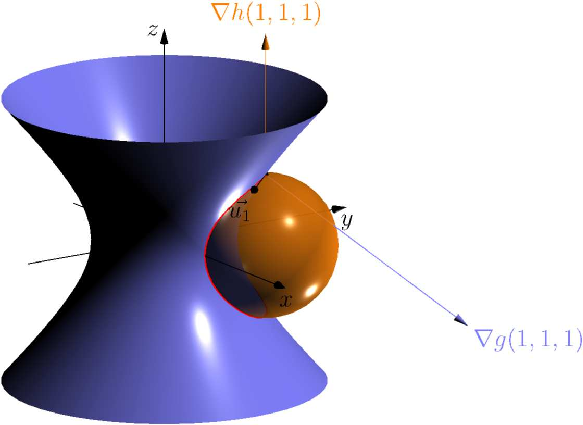
\includegraphics[width=\linewidth]{generated/asymptote/gabp2aq2-2022.pdf}
\end{image}%
\tcblower
\end{figureptx}%
\end{divisionexercise}%
\begin{divisionexercise}{3}{}{}{exercise-p2q3a-2022}%
Determine os pontos críticos da função%
\begin{equation*}
f(x,y) = x^2y +xy^2
-xy
\end{equation*}
e classifique-os como pontos de máximo local, mínimo local ou de sela.\par\smallskip%
\noindent\textbf{\blocktitlefont Resposta}.\hypertarget{answer-p2q3a-2022-b}{}\quad{}Os pontos \((0,0)\), \((1,0)\) e \((0,1)\) são de sela, enquanto que \((1/3,1/3)\) é de mínimo local.%
\par\smallskip%
\noindent\textbf{\blocktitlefont Solução}.\hypertarget{solution-p2q3a-2022-c}{}\quad{}Note que \(f\) é de classe \(\mathscr{C}^2\) e seu gradiente é%
\begin{equation*}
\nabla f(x,y) = (2xy+y^2 -y, 2xy+x^2 - x).
\end{equation*}
Deste modo, os pontos críticos de \(f\) são as soluções do sistema%
\begin{equation*}
\begin{cases} 2xy+y^2-y&=0,\\
2xy+x^2-x&=0.\end{cases}
\end{equation*}
A primeira equação equivale a \(y=0\) ou \(y=1-2x\). Vamos analisar os dois casos:%
\begin{itemize}[label=\textbullet]
\item{}substituindo \(y=0\) na segunda equação, obtemos \(x^2-x=0\), isto é, \(x=0\) ou \(x=1\). Temos, assim, os pontos \((0,0)\) e \((1,0)\);%
\item{}substituindo \(y=1-2x\) na segunda equação, obtemos \(-3x^2+x=0\), isto é, \(x=0\) ou \(x=1/3\). Para \(x=0\) temos \(y=1\); para \(x=1/3\) temos \(y=1/3\). Isto nos dá os pontos \((0,1)\) e \((1/3,1/3)\).%
\end{itemize}
%
\par
Uma vez encontrados os pontos críticos de \(f\), vamos classificá-los usando o Critério da Hessiana (\hyperref[theorem-teo_hess]{Teorema~{\xreffont\ref{theorem-teo_hess}}}). Precisamos das derivadas de segunda ordem de \textdollar{}f\textdollar{}:%
\begin{equation*}
\frac{\partial^2 f}{\partial x^2}(x,y) = 2y, \quad
\frac{\partial^2 f}{\partial y\partial x}(x,y) = 2x+2y-1, \quad
\frac{\partial^2 f}{\partial y^2}(x,y) = 2x.
\end{equation*}
Denotando por \(H_f(x,y)\) a matriz Hessiana de \(f\) no ponto \((x,y)\), temos:%
\begin{itemize}[label=\textbullet]
\item{}\(\det H_f(0,0) = \det\begin{bmatrix} 0 &
-1\\ -1 & 0 \end{bmatrix} = -1 < 0 \implies (0,0)\) é ponto de sela de \(f\).%
\item{}\(\det H_f(1,0) = \det\begin{bmatrix} 0 & 1\\ 1 & 2
\end{bmatrix} = -1 < 0 \implies (1,0)\) é ponto de sela de \(f\).%
\item{}\(\det H_f(0,1) = \det\begin{bmatrix} 2 & 1\\ 1 & 0 \end{bmatrix} =
-1 < 0 \implies (0,1)\) é ponto de sela de \(f\).%
\item{}\(\det H_f(1/3,1/3) = \det\begin{bmatrix} 2/3 & 1/3\\ 1/3 & 2/3
\end{bmatrix} = 1/3 > 0\) e \(\dfrac{\partial^2
f}{\partial x^2}(1/3,1/3) = 2/3> 0 \implies (1/3,1/3)\) é ponto de mínimo local de \(f\).%
\end{itemize}
%
\end{divisionexercise}%
\begin{divisionexercise}{4}{}{}{exercise-p2q4a-2022}%
Seja \(f\colon\R^3\to\R\) dada por \(f(x,y,z)=(x+y)z\). Determine o valor máximo e o valor mínimo de \(f\) em%
\begin{equation*}
C= \big\{ (x,y,z) \in \R^3\colon x^2 + y^2 -
z^2 = 1\text{ e } (x-1)^2 + (y-1)^2 +z^2 =1\big\}.
\end{equation*}
\par\smallskip%
\noindent\textbf{\blocktitlefont Resposta}.\hypertarget{answer-p2q4a-2022-b}{}\quad{}O valor máximo de \(f\) é \(2\), atingido no ponto \((1,1,1)\), enquanto o mínimo é \(-2\), atingido no ponto \((1,1,-1)\).\par\smallskip%
\noindent\textbf{\blocktitlefont Solução}.\hypertarget{solution-p2q4a-2022-c}{}\quad{}Observamos, primeiramente, que \(f\) é contínua e \(C\) é compacto (é a intersecção de um hiperboloide de uma folha, que é fechado, e uma esfera, que é fechada e limitada). O Teorema de Weierstrass assegura então que o problema proposto tem solução.%
\par
Usando a mesma notação da solução do \hyperlink{exercise-p2q2a-2022}{Exercício~{\xreffont 3.2.2}}, vamos considerar as funções \(g,h\colon\R^3\to\R\) dadas por%
\begin{equation*}
g(x,y,z) = x^2 + y^2 - z^2 \quad\text{e}\quad h(x,y,z) =
(x-1)^2 + (y-1)^2 + z^2.
\end{equation*}
As funções \(f\), \(g\) e \(h\) são de classe \(\mathscr{C}^1\) e seus gradientes são \(\nabla f(x,y,z) = (z,z, x+y)\), \(\nabla g(x,y,z) =
2(x,y,-z)\) e \(\nabla h(x,y,z) = 2 (x-1, y-1, z)\).%
\par
O Método dos Multiplicadores de Lagrange (\hyperref[theorem-teo_lag32]{Teorema~{\xreffont\ref{theorem-teo_lag32}}}) garante que os candidatos a máximos e mínimos locais de \(f\) em \(C\) são as soluções do sistema%
\begin{equation*}
\begin{cases} \{ \nabla f(x,y,z), \nabla g(x,y,z),
\nabla h(x,y,z)\}\; \text{é linearmente dependente},\\ x^2 +
y^2 - z^2 = 1,\\ (x-1)^2 +(y-1)^2+ z^2 = 1.  \end{cases}
\end{equation*}
A primeira condição equivale a%
\begin{equation*}
\det\begin{bmatrix} z & z
& x+y\\ x & y & -z\\ x-1 & y-1 & z
\end{bmatrix} = 0 \iff 2z^2(y-x)+y^2 - x^2 = 0,
\end{equation*}
ou seja, \((2z^2 + x+ y)(y-x)=0\), de modo que \(x=y\) ou \(x+y+2z^2=0\). Vamos analisar estes dois casos.%
%
\begin{itemize}[label=\textbullet]
\item{}Caso 1 \(x=y\). Substituindo isso nas outras duas equações temos%
\begin{equation*}
\begin{cases}
2x^2 - z^2 &= 1,\\
2(x-1)^2 + z^2 &= 1.
\end{cases}
\end{equation*}
Somando estas equações, concluímos que%
\begin{equation*}
x^2 - x = 0
\implies x = 0\; \text{ou}\; x = 1.
\end{equation*}
%
\par
Se \(x=0\), então \(y=0\) e \(z^2 + 1 = 0\), um absurdo. Se \(x=1\), então \(y=1\) e%
\begin{equation*}
z^2 = 1 \implies
z = \pm 1.
\end{equation*}
Isto nos dá os candidatos \((1,1,1)\) e \((1,1,-1)\).%
\item{}Caso 2 \(2z^2+x+y=0\). Somando as duas últimas equações obtemos \(x^2+y^2=x+y\) que, junto com a hipótese desse caso, prodduz \(x^2+y^2+2z^2=0\), ou seja, \((x,y,z)=(0,0,0)\). Este ponto não atende às restrições do problema (duas últimas equações do sistema de Lagrange).%
\end{itemize}
Com isso, os únicos candidatos são \((1,1,1)\) e \((1,1,-1)\), onde \(f(1,1,1)=(1+1)\cdot 1=2\) é valor máximo e \(f(1,1,-1)=(1+1)\cdot (-1)=-2\) é o valor mínimo.%
\par
Observamos que o problema poderia ser resolvido parametrizando-se a curva \(C\) e analisando a derivada de sua composta com a função \(f\).%
\end{divisionexercise}%
\end{exercises-subsection-numberless}
\end{sectionptx}
%
%
\typeout{************************************************}
\typeout{Seção 3.3 Prova Substitutiva}
\typeout{************************************************}
%
\begin{sectionptx}{Seção}{Prova Substitutiva}{}{Prova Substitutiva}{}{}{section-sec_2022-psub}
%
%
\typeout{************************************************}
\typeout{Exercícios 3.3 Exercícios}
\typeout{************************************************}
%
\begin{exercises-subsection-numberless}{Exercícios}{Exercícios}{}{Exercícios}{}{}{exercises-gab_psub-2022}
\begin{divisionexercise}{1}{}{}{exercise-psubq1a-2022}%
Considere a função \(f\colon\R^2\to\R\) dada por%
\begin{equation*}
f(x,y)=
\begin{cases}
\dfrac{x^3-y^3}{x^2+y^2},&\text{ se } (x,y) \neq (0,0),\\
\hfill 0,&\text{ se } (x,y)=(0,0).
\end{cases}
\end{equation*}
%
\begin{enumerate}[label=\alph*.]
\item{}Decida se \(f\) é contínua em \((0,0)\).%
\item{}Calcule as derivadas parciais de \(f\) em \((0,0)\).%
\item{}Decida se \(f\) é diferenciável em \((0,0)\).%
\item{}Calcule \(\dfrac{\partial f}{\partial \vec{u}}(0,0)\) sendo \(\vec{u} =(a,b)\) um vetor unitário.%
\end{enumerate}
%
\par\smallskip%
\noindent\textbf{\blocktitlefont Resposta}.\hypertarget{answer-psubq1a-2022-b}{}\quad{}%
\begin{enumerate}[label=\alph*.]
\item{}Sim, é contínua em \((0,0)\);%
\item{}\(f_x(0,0)=1\) e \(f_y(0,0)=-1\).%
\item{}Não é diferenciável em \((0,0)\).%
\item{}\(\dfrac{\partial f}{\partial \vec{u}}(0,0)=a^3-b^3\).%
\end{enumerate}
%
\par\smallskip%
\noindent\textbf{\blocktitlefont Solução}.\hypertarget{solution-psubq1a-2022-c}{}\quad{}Resolveremos cada item usando as definições.%
\par
%
\begin{enumerate}[label=\alph*.]
\item{}Basta usar o \hyperref[theorem-teo_limcont]{Teorema~{\xreffont\ref{theorem-teo_limcont}}} e verificar que%
\begin{align*}
\lim_{(x,y) \to (0,0)} f(x,y) &=
\lim_{(x,y) \to (0,0)}\frac{x^3-y^3}{x^2+y^2}\\
&=\lim_{(x,y)\to (0,0)} \left( \underbrace{x}_{\to 0}
\underbrace{\frac{x^2}{x^2+y^2}}_{\text{limitado}} -
\underbrace{y}_{\to 0}
\underbrace{\frac{y^2}{x^2+y^2}}_{\text{limitado}}\right)\\
&=0=f(0,0),
\end{align*}
para concluir que \(f\) é contínua em \((0,0)\).%
\item{}O denominador da primeira expressão que define \(f\) se anula em \((0,0)\), então não podemos usar as regras de derivação. Procedemos utilizando a \hyperref[definition-def_derpar]{Definição~{\xreffont\ref{definition-def_derpar}}}:%
\begin{align*}
f_x(0,0)=\dfrac{\partial f}{\partial x}(0,0) &=
\lim_{t \to 0} \frac{f(t,0) -f(0,0)}{t} = \lim_{t \to 0}
\frac{{t^3}/{t^2}}{t} = 1,\\
f_y(0,0)=\dfrac{\partial f}{\partial y}(0,0) &=
\lim_{t \to 0} \frac{f(0,t) -f(0,0)}{t} = \lim_{t \to 0}
\frac{{-t^3}/{t^2}}{t} = -1.
\end{align*}
%
\item{}Devemos determinar se o limite%
\begin{equation*}
\lim_{(h,k)\to (0,0)}
\frac{f(h,k)-f(0,0) - f_x(0,0)h - f_y(0,0)k}{\sqrt{h^2+k^2}} =
\lim_{(h,k) \to (0,0)} \frac{h^2k -
hk^2}{(h^2+k^2)^{3/2}}
\end{equation*}
existe e é igual a zero. Através da curva \(\alpha\colon\R\to\R^2\) dada por \(\alpha(t) = (-t,t)\), este limite se torna%
\begin{equation*}
\lim_{t
\to 0} \frac{2t^3}{2t^2 \sqrt{2t^2}} = \lim_{t \to 0}
\frac{t}{\sqrt{2}|t|},
\end{equation*}
que não existe (os limites laterais não coincidem). Isso implica que o limite original também não existe e, portanto, \(f\) não é diferenciável em \((0,0)\).%
\item{}Dado \(\vec{u}=(a,b)\) unitário, temos%
\begin{equation*}
\dfrac{\partial
f}{\partial \vec{u}}(0,0) = \lim_{t \to 0} \frac{f(ta,tb)
-f(0,0)}{t} = \lim_{t \to 0}
\frac{1}{t}\frac{t^3(a^3-b^3)}{t^2(a^2+b^2)} = a^3 - b^3,
\end{equation*}
pois \(a^2+b^2 = 1\). Convém observar que não podemos simplesmente tomar o produto interno do gradiente de \(f\) em \((0,0)\) pelo vetor \(\vec{u}\) porque \(f\) não é diferenciável em \((0,0)\)!%
\end{enumerate}
%
\par
Apresentamos outra solução possível do item (c) usando os itens (b) e (d). Caso \(f\) fosse diferenciável em \((0,0)\), teríamos%
\begin{equation*}
\frac{\partial f}{\partial
\vec{u}}(0,0) = \big\langle \nabla f(0,0), \vec{u}\big\rangle =
\big\langle (1,-1), (a,b)\big\rangle= a-b.
\end{equation*}
Assim, para provar que \(f\) não é diferenciável é suficiente exibir um vetor unitário \(\vec{u}=(a,b)\) tal que \(a^3 - b^3 \neq a
- b\) como, por exemplo, \(\vec{u} = \Big(
\dfrac{\sqrt{2}}{2}, -\dfrac{\sqrt{2}}{2}\Big)\) (verifique).%
\end{divisionexercise}%
\begin{divisionexercise}{2}{}{}{exercise-psubq2a-2022}%
Considere a função \(f(x, y) = x^2 + y^2 - 2kxy\), sendo \(k\) um número real. Para cada valor de \(k\), determine todos os pontos críticos de \(f\) e classifique-os.%
\par\smallskip%
\noindent\textbf{\blocktitlefont Resposta}.\hypertarget{answer-psubq2a-2022-b}{}\quad{}%
\begin{itemize}[label=\textbullet]
\item{}\(k=1\): \((x,x)\), \(x\in\R\) são os únicos pontos críticos, os quais são pontos de mínimo (globais) de \(f\).%
\item{}\(k=-1\): \((x,-x)\), \(x\in\R\) são os únicos pontos críticos, os quais são pontos de mínimo (globais) de \(f\).%
\item{}\(|k|<1\): \((0,0)\) é o único ponto crítico, o qual é um ponto de mínimo (global) de \(f\).%
\item{}\(|k|>1\): \((0,0)\) é o único ponto crítico, o qual é um ponto de sela de \(f\).%
\end{itemize}
%
\par\smallskip%
\noindent\textbf{\blocktitlefont Solução}.\hypertarget{solution-psubq2a-2022-c}{}\quad{}Como, para todo \(k\in\R\), a função \(f\) é de classe \(\mathscr{C}^2\) em todo o plano vamos utilizar o critério do Hessiano (\hyperref[theorem-teo_hess]{Teorema~{\xreffont\ref{theorem-teo_hess}}}). Para isso precisamos de suas derivadas até segunda ordem, indicadas convenientemente no vetor gradiente e matriz Hessiana:%
\begin{equation*}
\nabla f(x,y)=(2x-2ky,2y-2kx)\quad\text{e}\quad H_f(x,y)=
\begin{bmatrix}
2 & -2k\\ -2k & 2
\end{bmatrix}
\end{equation*}
%
\par
Os pontos críticos de \(f\) são aqueles que anulam o gradiente e portanto as soluções do sistema%
\begin{equation*}
\begin{cases}
x&=ky,\\ y&=kx.  \end{cases}
\end{equation*}
Subsituindo a segunda equação na primeira, temos%
\begin{equation*}
x=k^2 x \implies (k^2 - 1)x=0 \implies k = \pm 1\quad
\text{ou}\quad x = 0.
\end{equation*}
%
\par
Temos então três casos as considerar:%
\begin{itemize}[label=\textbullet]
\item{}\(k=1\): nesse caso temos%
\begin{equation*}
f(x,y)=x^2+y^2-2xy=(x-y)^2\geq 0,
\end{equation*}
para todos \((x,y)\in\R^2\). Aqui os pontos críticos satisfazem \(y=x\) e o determinante da matriz Hessiana se anula, não permitindo a aplicação do critério. Por outro lado,%
\begin{equation*}
f(x,x)=0\leq(x-y)^2=f(x,y)\text{,}
\end{equation*}
mostrando que todos os pontos da forma \((x,x)\), \(x\in\R\) são pontos de mínimo global de \(f\).%
\item{}\(k=-1\): agora%
\begin{equation*}
f(x,y)=x^2+y^2+2xy=(x+y)^2\geq
0,
\end{equation*}
para todos \((x,y)\in\R^2\). Aqui os pontos críticos satisfazem \(y=-x\) e o determinante da matriz Hessiana novamente se anula. Mas%
\begin{equation*}
f(x,-x)=0\leq(x+y)^2=f(x,y)\text{,}
\end{equation*}
mostrando que todos os pontos da forma \((x,x)\), \(x\in\R\) são pontos de mínimo global de \(f\).%
\item{}\(k\neq\pm 1\) e \(x=0\): isso garante que \(y=0\) e portanto o ponto \((0,0)\) é crítico para qualquer \(k\in\R\). Nesse caso temos%
\begin{equation*}
\det
H_f(0,0)=4(1-k^2)\quad\text{e}\quad f_{xx}(0,0)=2
\end{equation*}
e então quando \(|k|< 1\) a origem é um ponto de mínimo local, enquanto que \(|k|> 1\) garante a origem como um ponto de sela.%
\end{itemize}
%
\par
Veja os gráficos da função para alguns valores de \(k\):%
\begin{sidebyside}{2}{0}{0}{0}%
\begin{sbspanel}{0.5}[center]%
\begin{panelfigureptx}{Figura}{Gráfico de \(f\) para \(k=1\)}{figure-fig_gabpsubq21-2022}{}%
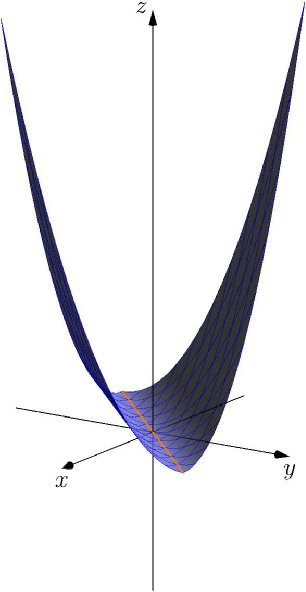
\includegraphics[width=\linewidth]{generated/asymptote/gabpsubq21-2022.pdf}
\tcblower
\end{panelfigureptx}%
\end{sbspanel}%
\begin{sbspanel}{0.5}[center]%
\begin{panelfigureptx}{Figura}{Gráfico de \(f\) para \(k=-1\)}{figure-fig_gabpsubq22-2022}{}%
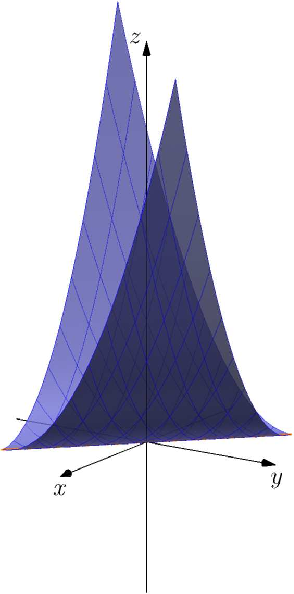
\includegraphics[width=\linewidth]{generated/asymptote/gabpsubq22-2022.pdf}
\tcblower
\end{panelfigureptx}%
\end{sbspanel}%
\end{sidebyside}%
\begin{sidebyside}{2}{0}{0}{0}%
\begin{sbspanel}{0.5}[center]%
\begin{panelfigureptx}{Figura}{Gráfico de \(f\) para \(k=\dfrac{1}{2}\)}{figure-fig_gabpsubq23-2022}{}%
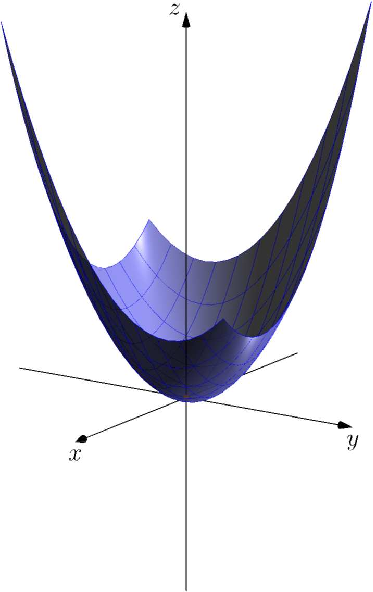
\includegraphics[width=\linewidth]{generated/asymptote/gabpsubq23-2022.pdf}
\tcblower
\end{panelfigureptx}%
\end{sbspanel}%
\begin{sbspanel}{0.5}[center]%
\begin{panelfigureptx}{Figura}{Gráfico de \(f\) para \(k=-\dfrac{1}{2}\)}{figure-fig_gabpsubq24-2022}{}%
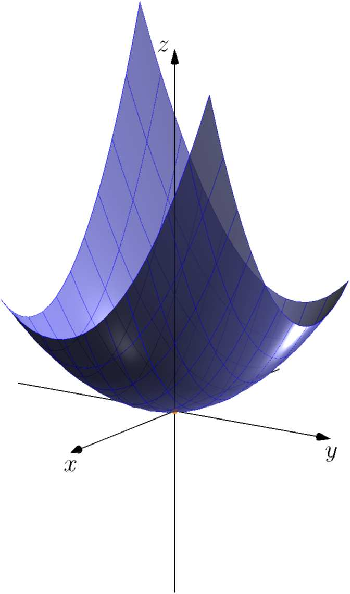
\includegraphics[width=\linewidth]{generated/asymptote/gabpsubq24-2022.pdf}
\tcblower
\end{panelfigureptx}%
\end{sbspanel}%
\end{sidebyside}%
\begin{sidebyside}{2}{0}{0}{0}%
\begin{sbspanel}{0.5}[center]%
\begin{panelfigureptx}{Figura}{Gráfico de \(f\) para \(k=-2\)}{figure-fig_gabpsubq25-2022}{}%
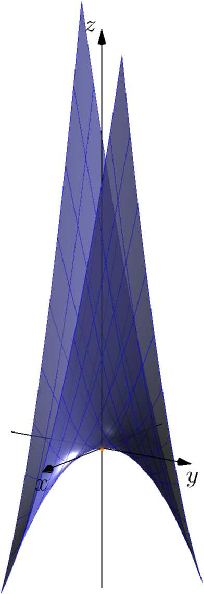
\includegraphics[width=\linewidth]{generated/asymptote/gabpsubq25-2022.pdf}
\tcblower
\end{panelfigureptx}%
\end{sbspanel}%
\begin{sbspanel}{0.5}[center]%
\begin{panelfigureptx}{Figura}{Gráfico de \(f\) para \(k=2\)}{figure-fig_gabpsubq26-2022}{}%
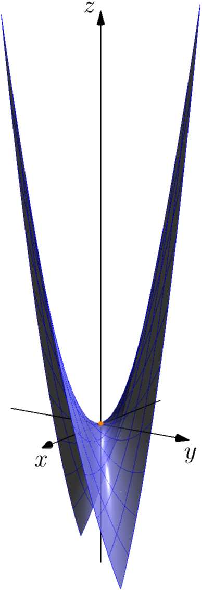
\includegraphics[width=\linewidth]{generated/asymptote/gabpsubq26-2022.pdf}
\tcblower
\end{panelfigureptx}%
\end{sbspanel}%
\end{sidebyside}%
\par
E por que não uma animação no Geogebra?%
\begin{figureptx}{Figura}{Gráfico de \(f\) para diversos valores de \(k\)}{figure-fig_gabpsubq2ggb-2022}{}%
\begin{sidebyside}{2}{0.075}{0.075}{0.17}%
\begin{sbspanel}{0.47}%
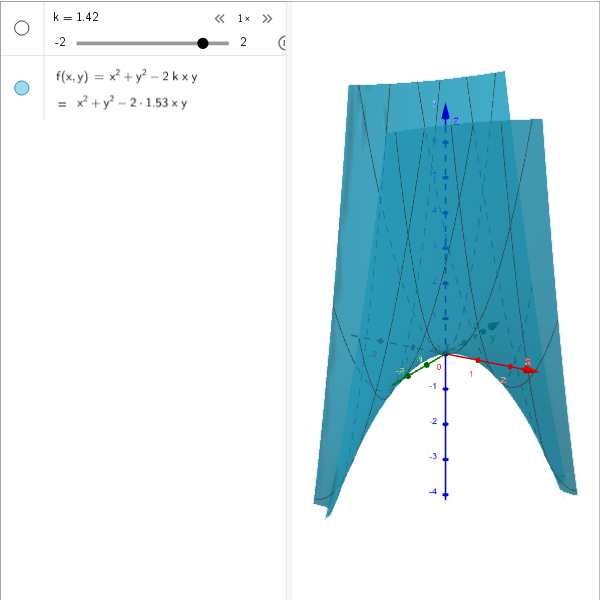
\includegraphics[width=\linewidth]{generated/preview/interactive-1-preview.png}
\end{sbspanel}%
\begin{sbspanel}{0.21}%

\includegraphics[width=\linewidth]{generated/qrcode/interactive-1.png}
\end{sbspanel}%
\end{sidebyside}%
\tcblower
\end{figureptx}%
\end{divisionexercise}%
\begin{divisionexercise}{3}{}{}{exercise-psubq3a-2022}%
Seja \(f\colon\R\to\R\) uma função diferenciável. Sabe-se que:%
\begin{enumerate}[label=(\roman*)]
\item{}A imagem da curva \(\sigma(t)=(e^{t-1}, -1 +
e^{2t-2})\), \(t\in\R\) está contida na curva de nível \(1\) de \(f\).%
\item{}A imagem da curva \(\gamma(u) = (2+u, 4(u+1), u^2)\), \(u\in\R\) está contida no gráfico de \(f\).%
\end{enumerate}
%
\par
Determine a equação do plano tangente ao gráfico de \(f\) no ponto \(\big(1,0,f(1,0)\big)\). Explicite claramente \(f(1,0)\) e \(\nabla f(1,0)\).%
\par\smallskip%
\noindent\textbf{\blocktitlefont Resposta}.\hypertarget{answer-psubq3a-2022-b}{}\quad{}\(f(1,0)=1\), \(\nabla f(1,0)=(2,-1)\) e \(\pi\colon
z=2x-y-1\).%
\par\smallskip%
\noindent\textbf{\blocktitlefont Solução}.\hypertarget{solution-psubq3a-2022-c}{}\quad{}Para calcular \(f(1,0)\) podemos usar as informações dadas em qualquer um dos itens (i) e (ii) do enunciado. De (i) temos que%
\begin{equation*}
f\big(\sigma(t)\big) = 1, \forall t \in \mathbb{R}.
\end{equation*}
Em particular, para \(t=1\), temos%
\begin{equation*}
\sigma(1) = (1,0)
\implies \boxed{f(1,0) = 1}.
\end{equation*}
%
\par
De (ii) segue-se que%
\begin{equation*}
f(2+u, 4(u+1))=u^2, \forall u \in
\mathbb{R}
\end{equation*}
e, tomando \(u=-1\), obtemos%
\begin{equation*}
\boxed{f(1,0) =
(-1)^2 = 1}.
\end{equation*}
%
\par
Nosso próximo passo é calcular o gradiente de \(f\) em \((1,0)\). Para isso derivamos as expressões acima com a regra da cadeia:%
\begin{equation*}
\begin{cases}
f\big(\sigma(t)\big)& = 1\\
f(2+u, 4(u+1))&=u^2
\end{cases}\implies
\begin{cases}
\Big\langle\nabla f\big(\sigma (t)\big),
\sigma'(t)\Big\rangle&=0\\
\Big\langle\nabla f\big(2+u, 4(u+1)\big),
(2+u, 4(u+1))'\Big\rangle&=2u\\
\end{cases}
\end{equation*}
%
\par
Escrevendo os vetores em coordenadas, substituindo \(t=1\) na primeira das equações do sistema acima e \(u=-1\) na segunda, temos%
\begin{equation*}
\begin{cases}
\dfrac{\partial f}{\partial x}(1,0) + 2 \dfrac{\partial
f}{\partial y}(1,0)&=0\\
\dfrac{\partial f}{\partial x}(1,0) + 4\dfrac{\partial f}{\partial
y}(1,0)&= -2.
\end{cases}
\end{equation*}
Resolvendo o sistema, encontramos%
\begin{equation*}
\boxed{\nabla f(1,0) = (2,-1)}
\end{equation*}
e, portanto, o plano tangente ao gráfico de \(f\) em \((1,0,1)\) tem equação%
\begin{equation*}
\pi\colon z=f(1,0) + \frac{\partial f}{\partial x}(1,0)(x-1) +
\frac{\partial f}{\partial y}(1,0)(y-0)\implies \pi\colon z= 2x-y-1.
\end{equation*}
%
\par
Uma figura para ilustrar a situação:%
\begin{figureptx}{Figura}{Cortes do gráfico de \(f\) e o plano tangente determinado por eles.}{figure-fig_gabpsubq3}{}%
\begin{image}{0}{1}{0}{}%
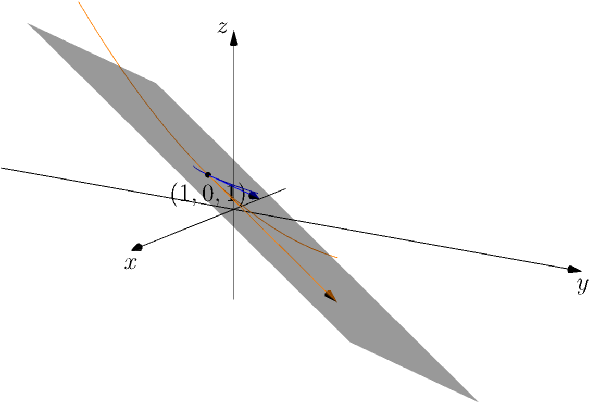
\includegraphics[width=\linewidth]{generated/asymptote/gabpsubq3.pdf}
\end{image}%
\tcblower
\end{figureptx}%
\end{divisionexercise}%
\begin{divisionexercise}{4}{}{}{exercise-psubq4a-2022}%
Determine o valor máximo e o valor mínimo de \(f(x,y,z)=y-z\) na elipse%
\begin{equation*}
C = \big\{(x,y,z)\in\R^3\colon
x^2 + y^2 - z^2 =0\text{ e } x+y-2z+1=0\big\}.
\end{equation*}
Explicite os pontos de \(C\) onde ocorrem esses valores.%
\par\smallskip%
\noindent\textbf{\blocktitlefont Resposta}.\hypertarget{answer-psubq4a-2022-b}{}\quad{}\(f(0,1,1)=0\) (máximo) e \(f(1,0,1)=-1\) (mínimo).%
\par\smallskip%
\noindent\textbf{\blocktitlefont Solução}.\hypertarget{solution-psubq4a-2022-c}{}\quad{}Vamos usar o Método dos Multiplicadores de Lagrange, com duas restrições. Outra opção, um tanto mais trabalhosa (precisaria saber eliminar termos mistos em equações de cônicas - uma aplicação de diagonalização de matrizes simétricas), seria parametrizar a elipse \(C\).%
\par
Sejam \(g,h\colon\R^3\to\R\) dadas por%
\begin{equation*}
g(x,y,z) = x^2
+ y^2 - z^2 \quad \text{e} \quad h(x,y,z) = x+y-2z.
\end{equation*}
Ambas são de classe \(\mathscr{C}^1\) e a elipse \(C\) é a intersecção da superfície de nível \(c=0\) de \(g\) e da superfície de nível \(c=-1\) de \(h\).%
\par
De acordo com o Método dos Multiplicadores de Lagrange, os candidatos são as soluções do sistema%
\begin{equation*}
\begin{cases}
\{\nabla f(x,y,z), \nabla g(x,y,z), \nabla h(x,y,z)\}\text{ é
linearmente dependente},\\
x^2 + y^2 - z^2 = 0,\\
x+y-2z+1=0.
\end{cases}
\end{equation*}
A primeira condição equivale a%
\begin{equation*}
\det\begin{bmatrix}
0 & 1 & -1\\
x & y & -z\\
1 & 1 &-2
\end{bmatrix} = 0 \iff x+ y -z=0.
\end{equation*}
%
\par
Subtraindo as equações \(x+ y -z =0\) e \(x+y-2z+1=0\) obtemos \textdollar{}z=1\textdollar{} e, portanto,%
\begin{equation*}
\begin{cases} x+y=1,\\ x^2 +
y^2=1, \end{cases}
\end{equation*}
o que implica que \(x=0\) e \(y=1\), ou \(x=1\) e \(y=0\).%
\par
Os candidatos são, portanto, os pontos%
\begin{equation*}
(0,1,1) \quad
\text{e} \quad (1,0,1),
\end{equation*}
nos quais \(f\) atinge, respectivamente, os valores \(f(0,1,1)=0\) (máximo) e \(f(1,0,1)=-1\) (mínimo).%
\par
Uma figura:%
\begin{figureptx}{Figura}{Cortes do gráfico de \(f\) e o plano tangente determinado por eles.}{figure-fig_gabpsubq4}{}%
\begin{image}{0}{1}{0}{}%
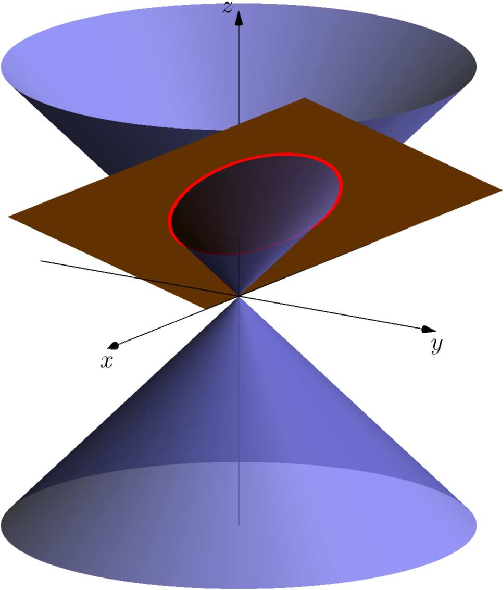
\includegraphics[width=\linewidth]{generated/asymptote/gabpsubq4.pdf}
\end{image}%
\tcblower
\end{figureptx}%
\end{divisionexercise}%
\end{exercises-subsection-numberless}
\end{sectionptx}
%
%
\typeout{************************************************}
\typeout{Seção 3.4 Prova de Recuperação}
\typeout{************************************************}
%
\begin{sectionptx}{Seção}{Prova de Recuperação}{}{Prova de Recuperação}{}{}{section-sec_2022-prec}
%
%
\typeout{************************************************}
\typeout{Exercícios 3.4 Exercícios}
\typeout{************************************************}
%
\begin{exercises-subsection-numberless}{Exercícios}{Exercícios}{}{Exercícios}{}{}{exercises-gab_prec-2022}
\begin{divisionexercise}{1}{}{}{exercise-precq1-2022}%
Considere a função \(f\colon\R^2\to\R\) dada por%
\begin{equation*}
f(x,y)=
\begin{cases}
\dfrac{x^{4/3}\sin(x^2)}{x^2+y^4},&\text{ se } (x,y) \neq (0,0),\\
\hfill 0,&\text{ se } (x,y)=(0,0).
\end{cases}
\end{equation*}
%
\begin{enumerate}[label=\alph*.]
\item{}Calcule as derivadas parciais de \(f\) em todos os pontos onde elas existirem.%
\item{}Decida se \(f\) é diferenciável em \((0,0)\).%
\item{}Calcule \(\dfrac{\partial f}{\partial \vec{u}}(0,0)\) sendo \(\vec{u} =(a,b)\) um vetor unitário.%
\end{enumerate}
%
\par\smallskip%
\noindent\textbf{\blocktitlefont Resposta}.\hypertarget{answer-precq1-2022-b}{}\quad{}%
\begin{enumerate}[label=\alph*.]
\item{}\(f_x(x,y)=
\begin{cases}
2\sqrt[3]{x}\dfrac{\Big(\frac{2}{3}\sin(x^2)+x^2\cos(x^2)\Big)
(x^2+y^4)-x^2\sin(x^2)}{(x^2+y^4)^2},&\text{ se } (x,y) \neq (0,0),\\
\hfill 0,&\text{ se } (x,y)=(0,0).
\end{cases}\) e \(f_y(x,y)=
\begin{cases}
\dfrac{x^{4/3}\sin(x^2)}{x^2+y^4},&\text{ se } (x,y) \neq (0,0),\\
\hfill 0,&\text{ se } (x,y)=(0,0).
\end{cases}\).%
\item{}É diferenciável em \((0,0)\).%
\item{}\(\dfrac{\partial f}{\partial \vec{u}}(0,0)=0\).%
\end{enumerate}
%
\par\smallskip%
\noindent\textbf{\blocktitlefont Solução}.\hypertarget{solution-precq1-2022-c}{}\quad{}%
\begin{enumerate}[label=\alph*.]
\item{}O denominador da primeira expressão que define \(f\) se anula em \((0,0)\), então não podemos usar as regras de derivação. Temos dois casos a tratar:%
\begin{itemize}[label=\textbullet]
\item{}\((x,y)\neq (0,0)\): qualquer desses pontos admite uma vizinhança onde \(f\) é dada pelo quociente de duas funções diferenciáveis, com denominador não nulo. Podemos aplicar diretamente a regra do quociente para cada variável:%
\begin{align*}
\dfrac{\partial f}{\partial x}(x,y)&
=2\sqrt[3]{x}\dfrac{\Big(\frac{2}{3}\sin(x^2)+x^2\cos(x^2)\Big)
(x^2+y^4)-x^2\sin(x^2)}{(x^2+y^4)^2}\\
\dfrac{\partial f}{\partial y}(x,y)
&=-\dfrac{4x^{4/3}\sin(x^2)y^3}{(x^2+y^4)^2}
\end{align*}
%
\item{}\((x,y)=(0,0)\): não podemos aplicar a regra do quociente, utilizada no caso anterior. É preciso seguir pela \hyperref[definition-def_derpar]{Definição~{\xreffont\ref{definition-def_derpar}}}:%
\begin{align*}
\dfrac{\partial f}{\partial x}(0,0) &
=\lim\limits_{h\to
0}\dfrac{f(0+h,0)-f(0,0)}{h}=\lim\limits_{h\to
0}\dfrac{\dfrac{h^{4/3}\sin(h^2)}{h^2+0^4}-0}{h}\\
&=\lim\limits_{h\to
0}\dfrac{\sin(h^2)}{h^{5/3}}=\lim\limits_{h\to
0}h^{1/3}\dfrac{\sin(h^2)}{h^2}=0.\\
\dfrac{\partial f}{\partial y}(0,0) &
=\lim\limits_{k\to 0}\dfrac{f(0,0+k)-f(0,0)}{k}=\lim\limits_{h\to
0}\dfrac{\dfrac{0^{4/3}\sin(0^2)}{0^2+k^4}-0}{k}\\
&=\lim\limits_{k\to
0}\dfrac{0}{k}=0.
\end{align*}
%
\end{itemize}
%
\item{}Já que as derivadas parciais de \(f\) existem em \((0,0)\), verificar sua diferenciabilidade nesse ponto requer o uso da definição, ou seja, verificar se existe e é nulo o limite%
\begin{align*}
\lim\limits_{(h,k)\to(0,0)}&\dfrac{f(0+h,0+k)-\dfrac{\partial
f}{\partial x}(0,0)h-f(0,0)-\dfrac{\partial
f}{\partial
y}(0,0)k}{\sqrt{h^2+k^2}}\\
&=\lim\limits_{(h,k)\to(0,0)}\dfrac{\dfrac{h^{4/3}\sin(h^2)}{h^2+k^4}
-0-0\cdot h-0\cdot k}{\sqrt{h^2+k^2}}\\
&=\lim\limits_{(h,k)\to(0,0)}h^{1/3}\dfrac{h}{\sqrt{h^2+k^2}}
\dfrac{\sin(h^2)}{h^2+k^4}\\
&=\lim\limits_{(h,k)\to(0,0)}h^{1/3}\dfrac{h}{\sqrt{h^2+k^2}}
\dfrac{\sin(h^2)}{h^2}\dfrac{h^2}{h^2+k^4}=0,
\end{align*}
pois o primeiro fator na expressão acima tende a \(0\), enquanto o terceito vai a \(1\) e o demais fatores são todos limitados.%
\par
Com isso mostramos que \(f\) é diferenciável na origem.%
\begin{remark}{Nota}{}{remark-precq1-2022-c-a-a-b-c}%
Outra opção seria tentar verificar a continuidade das derivadas parciais, mas atenção: caso isso não aconteça ainda assim a função pode ser diferenciável (e não de classe \(\mathscr{C}^1\)).\end{remark}
\item{}Em vista do item acima podemos usar a \hyperref[proposition-prop_derdir]{Proposição~{\xreffont\ref{proposition-prop_derdir}}}, obtendo%
\begin{equation*}
\dfrac{\partial
f}{\partial\vec{u}}(0,0)=\Big\langle\nabla
f(0,0),\vec{u}\Big\rangle=\big\langle(0,0),(a,b)\rangle=0.
\end{equation*}
%
\par
Caso nenhum dos itens anteriores fosse resolvido, poderíamos proceder pela \hyperref[definition-def_derdir]{Definição~{\xreffont\ref{definition-def_derdir}}}:%
\begin{align}
\dfrac{\partial
f}{\partial\vec{u}}(0,0)&=\lim\limits_{t\to
0}\dfrac{f\big((0,0)+t(a,b)\big)-f(0,0)}{t}\notag\\
&=\lim\limits_{t\to
0}\dfrac{\dfrac{(at)^{4/3}\sin\big((at)^2\big)}{(at)^2+(bt)^4}}{t}\tag{\textdagger}\label{mrow-preceq1}
\end{align}
%
\par
Se \(a=0\) então a expressão no limite acima é identicamente nula e temos \(\dfrac{\partial
f}{\partial\vec{u}}(0,0)=0\). Se \(a\neq 0\), então podemos escrever \hyperref[mrow-preceq1]{({\xreffont\ref{mrow-preceq1}})} como%
\begin{align*}
\dfrac{\partial
f}{\partial\vec{u}}(0,0)&=\lim\limits_{t\to
0}\dfrac{1}{a^2+b^4t^2}\,\dfrac{\sin(at)^2}{(at)^2}\,\dfrac{(at)^{10/3}}{t^3}\\
&=\lim\limits_{t\to
0}\dfrac{1}{a^2+b^4t^2}\,\dfrac{\sin(at)^2}{(at)^2}\,a^{10/3}t^{1/3}=0,
\end{align*}
pois o primeiro fator tende a \(1/a^2\), o segundo tende a \(1\) e o terceiro tende a \(0\).%
\end{enumerate}
%
\end{divisionexercise}%
\begin{divisionexercise}{2}{}{}{exercise-precq2-2022}%
Determine os pontos críticos de \(f(x,y)=
3x^2y+y^3-3x^2-3y^2+2\) e classifique-os. A função \(f\) tem ponto de máximo global? E mínimo global?%
\par\smallskip%
\noindent\textbf{\blocktitlefont Resposta}.\hypertarget{answer-precq2-2022-b}{}\quad{}Os pontos críticos são \(P_1=(0,0)\) (ponto de máximo local), \(P_2=(0,2)\) (ponto de mínimo local), \(P_3=(1,1)\) (ponto de sela) e \(P_1=(-1,1)\) (ponto de sela).%
\par\smallskip%
\noindent\textbf{\blocktitlefont Solução}.\hypertarget{solution-precq2-2022-c}{}\quad{}Os pontos críticos de \(f\) são, por definição, aqueles onde \(\nabla f(x,y)=(0,0)\). Isso nos dá o seguinte sistema%
\begin{equation*}
\begin{cases} 6xy-6x\amp=0\\ 3x^2+3y^2-6y\amp=0.  \end{cases}\iff
\begin{cases} 6x(y-1)\amp=0\\ 3x^2+3y^2-6y\amp=0.
\end{cases}
\end{equation*}
%
\par
Assim, temos dois casos a analisar:%
\begin{itemize}[label=\textbullet]
\item{}\(x=0\): na segunda equação isso diz que \(3y^2-6y=0\), ou seja, \(y=0\) ou \(y=2\). Temos então os pontos críticos \(\boxed{P_1=(0,0)}\) e \(\boxed{P_2=(0,2)}\).%
\item{}\(x\neq 0\): na primeira equação isso diz que \(y=1\) o que, na segunda equação, dá \(3x^2=3\), ou seja \(x=\pm
1\). Aparecem mais dois pontos críticos: \(\boxed{P_3=(1,1)}\) e \(\boxed{P_4=(-1,1)}\).%
\end{itemize}
%
\par
Para classificá-los, observamos que \(f\) é de classe \(\mathscr{C}^2\), e portanto podemos considerar a matriz Hessiana de \(f\), conforme o \hyperref[theorem-teo_hess]{Teorema~{\xreffont\ref{theorem-teo_hess}}}:%
\begin{equation*}
H_f(x,y)= \begin{bmatrix} f_{xx}(x,y)\amp f_{xy}(x,y)\\
f_{yx}(x,y)\amp f_{yy}(x,y) \end{bmatrix}= \begin{bmatrix}
6y-6\amp 6x\\
6x\amp 6y-6 \end{bmatrix},
\end{equation*}
cujo determinante é \(\det
H_f(x,y)=36\big((y-1)^2-x^2\big)\). Aplicando então o critério do Hessiano, temos%
\begin{itemize}[label=\textbullet]
\item{}\(H_f(P_1)=36\gt 0\) e \(f_{xx}(P_1)=-6\lt 0\), \(P_1\) é um ponto de máximo local.%
\item{}\(H_f(P_2)=36\gt 0\) e \(f_{xx}(P_2)=6\gt 0\), \(P_2\) é um ponto de mínimo local.%
\item{}\(H_f(P_3)=-36\lt 0\), \(P_3\) é um ponto de sela.%
\item{}\(H_f(P_4)=-36\lt 0\), \(P_4\) é um ponto de sela.%
\end{itemize}
%
\par
A função \(f\) não tem ponto de máximo global. De fato, olhando para a sua restrição de ao eixo \(Oy\), \(f(0,y)=y^3-3y^2\) verificamos que \(\lim\limits_{y\to+\infty}f(0,y)=+\infty\).%
\par
Ao longo do mesmo eixo temos que \(\lim\limits_{y\to-\infty}f(0,y)=-\infty\), mostrando que \(f\) também não tem ponto de mínimo global.%
\par
Veja o gráfico da função e, em destaque, os pontos do gráfico correspondentes aos pontos críticos encontrados:%
\begin{figureptx}{Figura}{Gráfico "re-escalado" de \(f\)}{figure-fig_gabrecq2-2022}{}%
\begin{image}{0.25}{0.5}{0.25}{}%
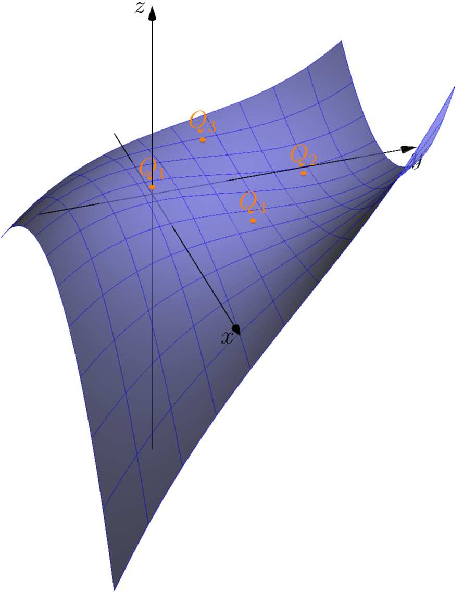
\includegraphics[width=\linewidth]{generated/asymptote/gabprecq2-2022.pdf}
\end{image}%
\tcblower
\end{figureptx}%
\end{divisionexercise}%
\begin{divisionexercise}{3}{}{}{exercise-precq3-2022}%
Sejam \(f\colon\R^2\to\R\) uma função diferenciável e \(g\colon\R^2\to\R\) dada por%
\begin{equation*}
g(x, y) = f (x^2 + 2y, x -
y^2).
\end{equation*}
%
\begin{enumerate}[label=\alph*.]
\item{}Sabendo que a direção de maior crescimento de \(f\) em \((5, -3)\) é a direção de \(\vec{v} = (1, 1)\), determine a equação da reta normal a curva de nível de \(g\) passando por \((1, 2)\).%
\item{}\emph{Item anulado}. A nota obtida nas demais questões foi multiplicada por \(20/17\).%
\end{enumerate}
%
\par\smallskip%
\noindent\textbf{\blocktitlefont Resposta}.\hypertarget{answer-precq3-2022-b}{}\quad{}\(r\colon (x,y)=(1,2)+\lambda (3,-2),\quad\lambda\in\R\)%
\par\smallskip%
\noindent\textbf{\blocktitlefont Solução}.\hypertarget{solution-precq3-2022-c}{}\quad{}%
\begin{enumerate}[label=\alph*.]
\item{}A direção de crescimento máximo de uma função em cada ponto é sempre a direção do gradiente da função nesse ponto (veja \hyperref[proposition-prop_crescmax]{Proposição~{\xreffont\ref{proposition-prop_crescmax}}}). Neste exercício, tal fato resume-se a dizer que \(\nabla f(5,-3)\) é paralelo a \(\vec{v}=(1,1)\).%
\par
Por outro lado, segue-se do \hyperref[corollary-cor_cadeiagradniv]{Corolário~{\xreffont\ref{corollary-cor_cadeiagradniv}}} que a reta normal à curva de nível de \(g\) que passa pelo ponto \((1,2)\) tem a direção de \(\nabla
g(1,2)\). Tendo o ponto e esta direção conseguimos construir a equação da reta pedida. Vamos determinar o gradiente de \(g\) em termos do gradiente de \(f\), usando a Regra da Cadeia (\hyperref[corollary-cor_cadeiaturbo]{Corolário~{\xreffont\ref{corollary-cor_cadeiaturbo}}}), pensando em \(f=f(u,v)\), com \(u(x,y)=x^2+2y\) e \(v(x,y)=x-y^2\), temos:%
\begin{align*}
g_x(x,y)\amp
=2xf_u(x^2+2y,x-y^2)+f_v(x^2+2y,x-y^2)\\
g_y(x,y)\amp
=2f_u(x^2+2y,x-y^2)-2yf_v(x^2+2y,x-y^2).
\end{align*}
%
\par
Fazendo \((x,y)=(1,2)\), temos \((u,v)=(5,-3)\). Além disso, a condição de paralelismo do primeiro parágrafo nos diz que \(f_u(5,-3)=f_v(5,-3)\). Chamemos esse valor de \(a=f_u(5,-3)\). Isto, nas equações acima, dá:%
\begin{align*}
g_x(1,2)\amp =2f_u(5,-3)+f_v(5,-3)=3a\\
g_y(1,2)\amp =2f_u(5,-3)-4f_v(5,-3)=-2a.
\end{align*}
%
\par
Assim, \(\nabla g(1,2)=(3a,-2a)\), que é paralelo ao vetor \((3,-2)\). Desta forma, a reta normal pedida é%
\begin{equation*}
\boxed{r\colon
(x,y)=(1,2)+\lambda (3,-2),\quad\lambda\in\R}.
\end{equation*}
%
\item{}\emph{Item anulado}.%
\end{enumerate}
\end{divisionexercise}%
\begin{divisionexercise}{4}{}{}{exercise-precq4-2022}%
Determine o maior volume que um paralelepípedo de faces paralelas aos planos coordenados e inscrito no elipsoide \(x^2+y^2 +4z^2 =1\) pode ter.%
\par\smallskip%
\noindent\textbf{\blocktitlefont Dica}.\hypertarget{hint-precq4-2022-b}{}\quad{}Basta encontrar um vértice de tal paralelepípedo que os demais ficam determinados.\par\smallskip%
\noindent\textbf{\blocktitlefont Resposta}.\hypertarget{answer-precq4-2022-c}{}\quad{}Os oito vértices do paralelepípedo são os pontos \(\Big(\pm\dfrac{\sqrt{3}}{3},\pm\dfrac{\sqrt{3}}{3},
\pm\dfrac{\sqrt{3}}{6}\Big)\), e o volume máximo é \(V=\dfrac{\sqrt{3}}{12}\).%
\par\smallskip%
\noindent\textbf{\blocktitlefont Solução}.\hypertarget{solution-precq4-2022-d}{}\quad{}Vamos usar o Método dos Multiplicadores de Lagrange, com uma restrição (\hyperref[theorem-teo_lag31]{Teorema~{\xreffont\ref{theorem-teo_lag31}}}). Outra opção, um tanto mais trabalhosa, seria eliminar uma das variáveis usando a equação do elipsoide, escrevendo o volume do paralelepípedo em termos das outras duas e estudar máximos e mínimos desse volume no compacto definido por essas duas variáveis. Em sua fronteira o volume será \(0\) e o valor máximo será atingido num ponto crítico (que está no interior). Estes pontos podem ser obtido com o método utilizado no \hyperlink{exercise-precq2-2022}{Exercício~{\xreffont 3.4.2}} (não precisa do teste com o Hessiano! Por que?).%
\par
As condições dadas no problema implicam que, se \((x,y,z)\) é o vértice de tal paralelepído no primeiro octante, então os demais vértices são obtidos com as sete comibinações restantes de sinais nas coordenadas.%
\par
O volume de tal paralelepípedo, se existir, será \(V(x,y,z)=|(2x)(2y)(2z)|=8|xyz|\), uma função contínua definida no elipsoide de equação \(x^2+y^2 +4z^2 =1\), que é compacto. Com isso o teorema de Weierstrass garante a existência do paralelepípedo pedido. Devido às simetrias observadas (ou à dica), podemos nos restringir apenas a valores positivos das variáveis, ou seja, o pedaço do elipsoide contido no primeiro quadrante (fechado). Aqui temos uma função a três variáveis que, da última observação escreve-se \(V(x,y,z)=8xyz\) (agora de classe \(\mathscr{C}^1\)), e desejamos encontrar seu ponto de máximo no elipsoide, que pode ser visto como a superfície de nível \(0\) da função \(g(x,y,z)=x^2+y^2+4z^2-1\). Utilizando-se a teoria de máximos e mínimos condicionados (multiplicadores de Lagrange), sabemos que os pontos \((x,y,z)\), de máximo ou mínimo local de \(V\) sobre \(g^{-1}(0)\), são aqueles onde%
\begin{equation*}
\begin{cases} \big\{\nabla V(x,y,z),\nabla
g(x,y,z)\big\}\amp\text{ é linearmente dependente}\\
g(x,y,z)\amp=0, \end{cases}
\end{equation*}
ou seja%
\begin{equation*}
\begin{cases}
\nabla V(x,y,z)\times\nabla g(x,y,z)\amp =\vec{0}\\ g(x,y,z)\amp
=0.  \end{cases}
\end{equation*}
%
\par
Aqui temos \(\nabla V(x,y,z)=8(yz,xz,xy)\) e \(\nabla
g(x,y,z)=2(x,y,4z)\) e então%
\begin{align*}
\nabla V(x,y,z)\times\nabla g(x,y,z)\amp =16 \left|\begin{vmatrix}
\vec{i}\amp\vec{j}\amp\vec{k}\\ yz\amp xz\amp xy\\ x\amp y\amp
4z\end{vmatrix}\right|\\
\amp
=16\big(x(4z^2-y^2),y(x^2-4z^2),z(y^2-x^2)\big).
\end{align*}
Explicitamente, o sistema torna-se então%
\begin{equation*}
\begin{cases}
x(4z^2-y^2)\amp =0\\ y(x^2-4z^2)\amp =0\\ z(y^2-x^2)\amp =0\\
x^2+y^2+4z^2\amp =1.  \end{cases}
\end{equation*}
%
\par
A solução completa do sistema resume-se a analisar os casos:%
\begin{itemize}[label=\textbullet]
\item{}\(x=0\): sob essa condição a segunda e terceira equação são equivalentes e dizem que \(y=0\) ou \(z=0\). Isso na última equação dá, repectivamete os candidatos \(\boxed{(0,0,1/2)}\) e \(\boxed{(0,1,0)}\). Em ambos a função volume é nula.%
\item{}\(y=0\): como acima, temos que \(x=0\) ou \(z=0\) e os pontos \(\boxed{(0,0,1/2)}\) e \(\boxed{(1,0,0)}\), nos quais o volume também é nulo.%
\item{}\(z=0\): aqui teremos que \(x=0\) ou \(y=0\), dando os pontos \(\boxed{(0,1,0)}\) e \(\boxed{(1,0,0)}\). Mais uma vez o volume se anula nesses candidatos.%
\item{}\(xyz\neq 0\): aqui as três primeiras equações dizem que \(x^2=y^2=4z^2\). Na última equação isso dá \(12z^2=1\), ou seja \(z=\sqrt{3}/6\), donde \(x=y=\sqrt{3}/3\). Nesse ponto o volume vale \(V=\sqrt{3}/12\), maior valor entre os candidatos viáveis e portanto solução do problema.%
\end{itemize}
%
\par
Por que não uma figura?%
\begin{figureptx}{Figura}{O paralelepípedo de volume máximo é o de tom alaranjado.}{figure-fig_gabrecq4-2022}{}%
\begin{image}{0.25}{0.5}{0.25}{}%
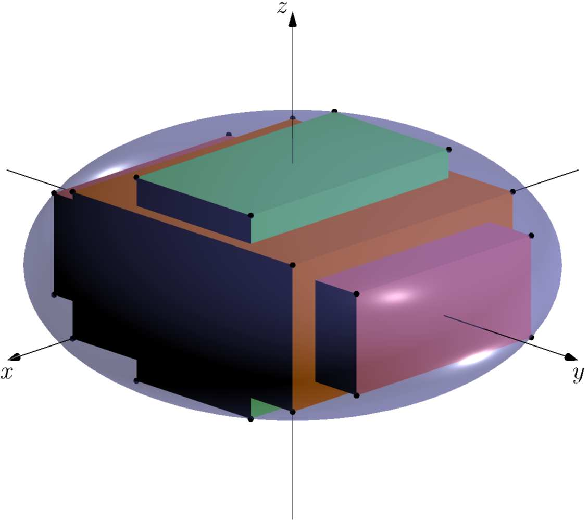
\includegraphics[width=\linewidth]{generated/asymptote/gabprecq4-2022.pdf}
\end{image}%
\tcblower
\end{figureptx}%
\end{divisionexercise}%
\end{exercises-subsection-numberless}
\end{sectionptx}
\end{chapterptx}
%
%
\typeout{************************************************}
\typeout{Capítulo 4 Provas de 2021}
\typeout{************************************************}
%
\begin{chapterptx}{Capítulo}{Provas de 2021}{}{Provas de 2021}{}{}{chapter-ch_2021}
\renewcommand*{\chaptername}{Capítulo}
\begin{introduction}{}%
Neste capítulo apresentamos as soluções dos exercícios das provas aplicadas em 2021, quando a Escola Politécnica optou por um calendário com duas provas. Durante o período de pandemia e isolamento, as provas foram aplicadas remotamente e algumas delas eram objetivas, enquanto outras eram abertas. O calendário da Universidade varia a cada ano e implica numa alteração do programa de cada avaliação.%
\par
A primeira prova aborda polinômios de Taylor em uma variável real, os conceitos de limites, continuidade, derivadas parciais, diferenciabilidade de funções a duas variáveis reais e regra da cadeia.%
\par
A segunda prova tem questões sobre derivadas de ordem superior, interseções de superfícies, polinômios de Taylor em várias variáveis, classificação de pontos críticos de uma função num abertos do plano e problemas de otimização com restrições (multiplicadores de Lagrange).%
\end{introduction}%
%
%
\typeout{************************************************}
\typeout{Seção 4.1 Primeira Prova}
\typeout{************************************************}
%
\begin{sectionptx}{Seção}{Primeira Prova}{}{Primeira Prova}{}{}{section-sec_2021-p1}
%
%
\typeout{************************************************}
\typeout{Exercícios 4.1 Exercícios}
\typeout{************************************************}
%
\begin{exercises-subsection-numberless}{Exercícios}{Exercícios}{}{Exercícios}{}{}{exercises-gab_2021-p1}
\begin{divisionexercise}{1}{}{}{exercise-p1q1-2021}%
Sejam \(f\) e \(g\) duas funções que admitem derivadas de qualquer ordem, tais que \(P_n\) e \(Q_n\) são os respectivos polinômios de Taylor de ordem \(n\) em torno de \(x_0=0\).%
\par
Assinale, dentre as alternativas abaixo, precisamente aquelas que são verdadeiras (marcar uma incorreta descontará nota).%
\begin{enumerate}[label=\alph*]
\item{}Se \(f\) é uma função par, então \(P_n\) é a soma de monômios com potências pares de \(x\).%
\item{}Se \(P_n(x)=Q_n(x)\), para algum \(n\), então \(f(x)=g(x)\).%
\item{}O polinômio de Taylor de ordem \(n\) para a função \(f(x)g(x)\), em torno de \(x_0=0\), é%
\begin{equation*}
f(0)g(0)+f'(0)g'(0)x+\dfrac{f''(0)g''(0)}{2!}x^2+\ldots+
\dfrac{f^{(n)}(0)g^{(n)}(0)}{n!}x^n.
\end{equation*}
%
\item{}Se \(R_n\) é o polinômio de Taylor de ordem \(n\) de \(f'\) em torno de \(x_0=0\), então \(R_n(x)=\dfrac{d}{dx}P_{n+1}(x)\).%
.\end{enumerate}
%
\par\smallskip%
\noindent\textbf{\blocktitlefont Resposta}.\hypertarget{answer-p1q1-2021-b}{}\quad{}%
\begin{enumerate}[label=\alph*]
\item{}Verdadeira%
\item{}Falsa%
\item{}Falsa%
\item{}Verdadeira%
\end{enumerate}
%
\par\smallskip%
\noindent\textbf{\blocktitlefont Solução}.\hypertarget{solution-p1q1-2021-c}{}\quad{}%
\begin{enumerate}[label=\alph*]
\item{}Se \(f\) é par, então \(f(-x)=f(x)\) que, derivando em \(x_0=0\), nos dá \(-f'(-0)=f'(0)\implies
f'(0)=0\), mostrando que o coeficiente de \(x\) em \(P_n\) é nulo. Repetindo esse argumento para todas as derivadas de ordem ímpar temos o resultado.%
\item{}Se \(f(x)=x\) e \(g(x)=\sin x\), então \(P_1(x)=x=Q_1(x)\) mas \(f(x)\neq g(x)\).%
\item{}Observe que a derivada de \(f(x)g(x)\) não é \(f'(x)g'(x)\) e portanto o coeficiente de um dado termo do polinômio de \(f(x)g(x)\) não é simplesmente o produto dos coeficientes. Caso concreto: considere \(f(x)=1\) e \(g(x)=\sin x\), então \(f(x)g(x)=\sin x=g(x)\) tem como polinômio de Taylor de ordem 3, centrado em \(x_0=0\), \(x-x^3/3!\) (o mesmo de \(g\)), mas aplicando a fórmula proposta teríamos o polinômio nulo.%
\item{}Observando que \(f^{(n+1)}(x_0)=(f')(n)(x_0)\) e que \(\dfrac{d}{dx}\left(\dfrac{(x-x0)^{k+1}}{(k+1)!}\right)=\dfrac{(x-x0)^k}{k!}\), segue-se que \(R_n(x)=\dfrac{d}{dx}P_{n+1}(x)\).%
\end{enumerate}
%
\end{divisionexercise}%
\begin{divisionexercise}{2}{}{}{exercise-p1q2-2021}%
Considere a curva \(\gamma(t)=\left(15\cos t,\dfrac{\sin
t}{2+\cos t}\right)\), \(t\in[0,2\pi]\), e o triângulo delimitado delimitado pelas retas tangentes à \(\gamma\) nos pontos \((-15,0)\),\((0,1/2)\) e \((0,-1/2)\). A área deste triângulo é:%
\begin{multicols}{5}
\begin{enumerate}[label=\alph*]
\item{}\(\displaystyle 15\)%
\item{}\(\displaystyle \dfrac{135}{2}\)%
\item{}\(\displaystyle \dfrac{15}{2}\)%
\item{}\(\displaystyle \dfrac{135}{4}\)%
\item{}\(\displaystyle \dfrac{45}{4}\)%
\end{enumerate}
\end{multicols}
%
\par\smallskip%
\noindent\textbf{\blocktitlefont Resposta}.\hypertarget{answer-p1q2-2021-b}{}\quad{}Alternativa d.%
\par\smallskip%
\noindent\textbf{\blocktitlefont Solução}.\hypertarget{solution-p1q2-2021-c}{}\quad{}Os pontos dados são atingidos pela curva quanto \(t=\pi\), \(t=\pi/2\) e \(t=3\pi/2\), respectivamente. Os vetores tangentes nesse pontos são \(\gamma'(\pi)=(0,-1)\), \(\gamma'(\pi/2)=(-15,1/4)\) e \(\gamma'(3\pi/2)=(15,1/4)\). Com isso, temos as retas tangentes%
\begin{equation*}
r1\colon x=-15,\quad r2\colon
x+60y=30\quad\text{e}\quad r3\colon x-60y=30\text{.}
\end{equation*}
As interseções são os pontos \((30,0)\), \((-15,3/4)\) e \((-15,-3/4)\), que formam um triângulo de altura \(45\) e base \(3/2\), com área \(135/4\). Veja a figura: \begin{figureptx}{Figura}{Imagem de \(\gamma\) e tangentes.}{figure-fig_gabp1q2-2021}{}%
\begin{image}{0.25}{0.5}{0.25}{}%
\resizebox{\linewidth}{!}{%
              \begin{tikzpicture}
              \draw[thick,->] (-2,0)--(3,0) node[below]{$x$};
              \draw[thick,->] (0,-1.5)--(0,1.5) node[right]{$y$};
\draw[domain=0:2*pi,red, samples=100] plot({cos(\x r)},{sin(\x
r)/(2+cos(\x r))});
\draw[blue] (-1,-1) -- (-1,1) node[left]{{$r_1$}};
\draw[olive] (-1.5,{{3.5/4}}) -- (2.5,{{-1/8}})
node[below]{{$r_2$}};
\draw[orange] (-1.5,{{-3.5/4}}) -- (2.5,{{1/8}})
node[above]{{$r_3$}}; 
              \end{tikzpicture}
}%
\end{image}%
\tcblower
\end{figureptx}%
%
\end{divisionexercise}%
\begin{divisionexercise}{3}{}{}{exercise-p1q3-2021}%
Considere a função \(f(x,y)=\dfrac{7(x-1)^2+2(y-1)^2}{x^2+y^2}\), definida em \(\R^2\setminus\big\{(0,0)\big\}\). As curvas de nível \(7\) e \(9/2\) são, respectivamente:%
\begin{enumerate}[label=\alph*]
\item{}um par de retas concorrentes e uma elipse.%
\item{}um par de retas paralelas e uma elipse.%
\item{}uma hipérbole e uma parábola.%
\item{}uma parábola e uma hipérbole.%
\item{}uma parábola e um par de retas concorrentes.%
\end{enumerate}
%
\par\smallskip%
\noindent\textbf{\blocktitlefont Resposta}.\hypertarget{answer-p1q3-2021-b}{}\quad{}Alternativa d.%
\par\smallskip%
\noindent\textbf{\blocktitlefont Solução}.\hypertarget{solution-p1q3-2021-c}{}\quad{}Escrevendo \(f(x,y)=k\), para \((x,y)\neq (0,0)\), temos%
\begin{equation*}
\dfrac{7(x-1)^2+2(y-1)^2}{x^2+y^2}=k\iff
(7-k)x^2-14x+(2-k)y^2-4y+9=0.
\end{equation*}
%
\par
Aplicando os valores de \(k\) indicados, a equação acima escreve-se%
\begin{itemize}[label=\textbullet]
\item{}\(k=7\): \(-14x-5y^2-4y+9=0\), ou seja \(x=\dfrac{9-4y-5y^2}{14}\), que descreve uma parábola.%
\item{}\(k=9/2\): \(\dfrac{5}{2}x^2-14x-\dfrac{5}{2}y^2-4y+9=0\) que completando quadrados, fica \(5(x-14/5)^2-5(y+4/5)^2=18\), isto é, uma hiperbole.%
\end{itemize}
%
\par
Veja ambas numa figura: \begin{figureptx}{Figura}{Curvas de nível para \(f(x,y)\).}{figure-fig_gabp1q3-2021}{}%
\begin{image}{0.25}{0.5}{0.25}{}%
\resizebox{\linewidth}{!}{%
              \begin{tikzpicture}
              \draw[thick,->] (-3,0)--(6,0) node[below]{$x$};
              \draw[thick,->] (0,-3)--(0,3) node[right]{$y$};
\draw[domain=-2.5:2.5,red, samples=100]
plot({(9-4*\x-5*(\x)^2)/14},{\x}) node[above]{$c=7$};
\draw[domain=-1:1,olive, samples=100]
plot({sqrt(18/5)*cosh(\x)+14/5},{sqrt(18/5)*sinh(\x)-4/5})
node[above]{$c=\frac{9}{2}$};
\draw[dashed] (14/5,-3)--(14/5,3);
\draw[dashed] (-3,-4/5)--(6,-4/5);
\draw[domain=-1:1,olive, samples=100]
plot({2*14/5-(sqrt(18/5)*cosh(\x)+14/5)},{sqrt(18/5)*sinh(\x)-4/5});
\end{tikzpicture}
}%
\end{image}%
\tcblower
\end{figureptx}%
%
\end{divisionexercise}%
\begin{divisionexercise}{4}{}{}{exercise-p1q4-2021}%
Seja \(f(x,y)\) uma função diferenciável em \((3,-2)\) tal que \(f(3,-2)=-3\). Sabe-se também que \(\dfrac{\partial
f}{\partial \vec{u}}(3,-2)=1\) e \(\dfrac{\partial
f}{\partial \vec{v}}(3,-2)=-2\), onde \(\vec{u}=\left(-\dfrac{1}{\sqrt{2}},\dfrac{1}{\sqrt{2}}\right)\) e \(\vec{v}=\left(\dfrac{1}{\sqrt{2}},\dfrac{1}{\sqrt{2}}\right)\). A equação do plano tangente ao gráfico de \(f\) no ponto \((3,-2,-3)\) é:%
\begin{equation*}
\boxed{\phantom{AAA}}x+\boxed{\phantom{AAA}}y-z+\boxed{\phantom{AAA}}=0.
\end{equation*}
%
\par
O valor máximo que uma derivada direcional de \(f\) no ponto \((3,-2)\) assume é \(\boxed{\phantom{AAA}}\).%
\par\smallskip%
\noindent\textbf{\blocktitlefont Resposta}.\hypertarget{answer-p1q4-2021-b}{}\quad{}\(\left(-\dfrac{3}{\sqrt{2}},-\dfrac{1}{\sqrt{2}},\dfrac{7\sqrt{2}-6}{2}\right)\).%
\par
\(\sqrt{5}\).%
\par\smallskip%
\noindent\textbf{\blocktitlefont Solução}.\hypertarget{solution-p1q4-2021-c}{}\quad{}Sabendo que \(f\) é diferenciável em \((x_0,y_0)=(3,-2)\) e dadas as derivadas direcionais no enunciado, podemos determinar \(\nabla f(3,-2)\) através do sistema de equações lineares%
\begin{equation*}
\begin{cases} \big\langle\nabla
f(3,-2),\vec{u}\big\rangle= \dfrac{\partial f}{\partial
\vec{u}}(3,-2)&=1\\ \big\langle\nabla
f(3,-2),\vec{v}\big\rangle= \dfrac{\partial f}{\partial
\vec{v}}(3,-2)&=-2, \end{cases}
\end{equation*}
que tem uma matriz de coeficientes ortogonal (fica fácil resolver) e encontrar \(\nabla
f(3,-2)=\left(-\dfrac{3}{\sqrt{2}},-\dfrac{1}{\sqrt{2}}\right),\) cujas coordenadas são, respectivamente, os coeficientes da equação do plano pedido, já que o coeficiente de \(z\) é \(-1\). O termo independente é \(d=f(x_0,y_0)-f_x(x_0,y_0)x_0-f_y(x_0,y_0)y_0=\dfrac{7\sqrt{2}-6}{2}\).%
\par
O valor máximo da derivada direcional é precisamente \(\|\nabla f(3,-2)\|=\sqrt{5}\).%
\end{divisionexercise}%
\begin{divisionexercise}{5}{}{}{exercise-p1q5-2021}%
Seja \(f\colon \R^2\to\R\) dada por \(f(x,y)=\max\Big\{\dfrac{x}{3+|y|},\dfrac{y}{3+|x|}\Big\}\).%
\par
O valor de \(\dfrac{\partial f}{\partial x}(0,0)\) é%
\begin{multicols}{5}
\begin{enumerate}[label=\alph*.]
\item{}\(0\).%
\item{}\(-\dfrac{1}{3}\).%
\item{}\(\dfrac{1}{3}\).%
\item{}3\(0\)%
\item{}inexistente.%
\end{enumerate}
\end{multicols}
%
\par
O valor de \(\dfrac{\partial f}{\partial x}(1,0)\) é%
\begin{multicols}{5}
\begin{enumerate}[label=\alph*.]
\item{}\(0\).%
\item{}\(-\dfrac{1}{3}\).%
\item{}\(\dfrac{1}{3}\).%
\item{}3\(0\)%
\item{}inexistente.%
\end{enumerate}
\end{multicols}
%
\par\smallskip%
\noindent\textbf{\blocktitlefont Dica}.\hypertarget{hint-p1q5-2021-b}{}\quad{}Lembre-se do significado conceitual da derivada parcial (não a definição) e tudo fica muito simples.%
\par\smallskip%
\noindent\textbf{\blocktitlefont Resposta}.\hypertarget{answer-p1q5-2021-c}{}\quad{}Alternativa e.%
\par
Alternativa c.%
\par\smallskip%
\noindent\textbf{\blocktitlefont Solução}.\hypertarget{solution-p1q5-2021-d}{}\quad{}Basta olhar para \(g(x)=f(x,0)=\max\Big\{\dfrac{x}{3},0\Big\}\) e observar que a existência e o valor de \(\dfrac{\partial f}{\partial
x}(x_0,0)\) são dados exatamente por \(g'(x_0)\).%
\par
Em \(x_0=0\), temos que \(g\) não é derivável:%
\begin{equation*}
\lim\limits_{h\to 0^+}\dfrac{g(h)-g(0)}{h}=\dfrac{1}{3}\neq
0=\lim\limits_{h\to 0^-}\dfrac{g(h)-g(0)}{h}.
\end{equation*}
%
\par
Já em \(x_0=0\), consideramos o limite%
\begin{equation*}
\lim\limits_{h\to
0}\dfrac{g(1+h)-g(1)}{h}=\dfrac{1}{3},
\end{equation*}
pois \(h\to 0\) nos permite considerar \(h>1\) e portanto \(g(1+h)=\dfrac{1+h}{3}\).%
\end{divisionexercise}%
\begin{divisionexercise}{6}{}{}{exercise-p1q6-2021}%
Sejam \(f\colon\R^2\to\R\) uma função e \((x_0,y_0)\in\R^2\). Assinale, dentre as alternativas abaixo, precisamente aquelas que são verdadeiras (marcar uma incorreta descontará nota):%
\begin{enumerate}[label=\alph*]
\item{}Se \(f\) não é diferenciável em \((x_0,y_0)\), então \(f\) não admite derivadas parciais em \((x_0,y_0)\).%
\item{}Se \(f\) não é diferenciável em \((x_0,y_0)\), então \(f\) não é contínua em \((x_0,y_0)\).%
\item{}Se \(f\) não é contínua em \((x_0,y_0)\), então \(f\) não admite derivadas parciais em \((x_0,y_0)\).%
\item{}Se \(f\) não admite derivadas parciais em \((x_0,y_0)\), então \(f\) não é diferenciável em \((x_0,y_0)\).%
\item{}Se \(f\) não é diferenciável em \((x_0,y_0)\), então \(f\) as derivadas parciais de \(f\) não são contínuas em \((x_0,y_0)\).%
\end{enumerate}
%
\par\smallskip%
\noindent\textbf{\blocktitlefont Resposta}.\hypertarget{answer-p1q6-2021-b}{}\quad{}%
\begin{enumerate}[label=\alph*]
\item{}Falsa%
\item{}Falsa%
\item{}Falsa%
\item{}Verdadeira%
\item{}Verdadeira%
\end{enumerate}
%
\par\smallskip%
\noindent\textbf{\blocktitlefont Solução}.\hypertarget{solution-p1q6-2021-c}{}\quad{}%
\begin{enumerate}[label=\alph*]
\item{}Falsa. A função \(f(x,y)=\begin{cases}
\dfrac{xy}{x^2+y^2},&\text{ se }(x,y)\neq (0,0)\\
\hfill 0,&\text{ se} (x,y)=(0,0)
\end{cases}\) admite as duas derivadas parciais na origem e não é sequer contínua ali, quando mais diferenciável.%
\item{}Falsa. O exemplo acima reflete isso.%
\item{}Falsa. Mais uma vez o mesmo exemplo ilustra isso.%
\item{}Verdadeira. Pois a definição de diferenciabilidade via limite exige a existência das derivadas parciais.%
\item{}Verdadeira. Se as derivadas parciais de \(f\) são contínuas num ponto, então \(f\) é diferenciável nesse ponto.%
\end{enumerate}
%
\end{divisionexercise}%
\begin{divisionexercise}{7}{}{}{exercise-p1q7-2021}%
Seja \(f\colon\R^2\to\R\) uma função diferenciável tal que \(f(sx,sy)=sf(x,y)\), para todos \((x,y)\in\R^2\) e \(s\in\R\). Se \(\nabla f(0,0)=(8,9)\), então \(f(7,3)\)%
\begin{enumerate}[label=\alph*]
\item{}vale \(83\)%
\item{}vale \(87\)%
\item{}não ode ser determinado a partir dos dados fornecidos%
\item{}vale \(0\)%
\item{}vale \(17\)%
\end{enumerate}
%
\par\smallskip%
\noindent\textbf{\blocktitlefont Dica}.\hypertarget{hint-p1q7-2021-b}{}\quad{}Use a regra da cadeia para \(f\) e o segmento que liga a origem até cada ponto \((x,y)\) do plano.%
\par\smallskip%
\noindent\textbf{\blocktitlefont Resposta}.\hypertarget{answer-p1q7-2021-c}{}\quad{}Alternativa a.%
\par\smallskip%
\noindent\textbf{\blocktitlefont Solução}.\hypertarget{solution-p1q7-2021-d}{}\quad{}Das hipóteses temos que \(sf(7,3)=f(7s,3s)\) e, derivando em relação a \(s\) temos \(f(7,3)=\big\langle\nabla
f(7s,3s),(7,3)\big\rangle\). Fazendo \(s=0\) vem que \(f(7,3)=83\).%
\end{divisionexercise}%
\begin{divisionexercise}{8}{}{}{exercise-p1q8-2021}%
Seja \(f\colon\R^2\to\R\) uma função diferenciável. Sabendo que \(7x+3y+2z+5=0\) é a equação do plano tangente ao gráfico de \(f\) no ponto \((2,3)\), determine:%
\begin{enumerate}[label=\alph*]
\item{}\(\displaystyle f(2,3)\)%
\item{}\(\displaystyle \nabla f(2,3)\)%
\item{}\(\dfrac{\partial f}{\partial\vec{u}}(2,3)\), onde \(\vec{u}\) é o versor do vetor \(\vec{v}=(3,2)\)%
\item{}a reta tangente ao gráfico da função \(g(t)=f(3\sin(t)+t^4+2,2\cos(t)+e^{-3t})\) no ponto de abscissa \(t_0=0\).%
\item{}o plano tangente ao gráfico de \(h(u,v)=uf(u+v,u-v)\) no ponto \(\big(5/2,-1/2,h(5/2,-1/2)\big)\).%
\end{enumerate}
%
\par\smallskip%
\noindent\textbf{\blocktitlefont Resposta}.\hypertarget{answer-p1q8-2021-b}{}\quad{}%
\begin{enumerate}[label=\alph*]
\item{}\(\displaystyle -14\)%
\item{}\(\displaystyle (-7/2.-3/2)\)%
\item{}\(\displaystyle -\dfrac{27}{2\sqrt{13}}\)%
\item{}\(\displaystyle y=-6x-14\)%
\item{}\(\displaystyle \pi\colon -\frac{53}{2}(x-5/2)-5(y+1/2)-z-35=0\)%
\end{enumerate}
\par\smallskip%
\noindent\textbf{\blocktitlefont Solução}.\hypertarget{solution-p1q8-2021-c}{}\quad{}%
\begin{enumerate}[label=\alph*]
\item{}Substituindo \((2,3)\) na equação do plano tangente dado temos \(f(2,3)=z=-14\).%
\item{}Da mesma equação do plano temos que \(\nabla
f(2,3)=(-7/2,-3/2)\).%
\item{}Inicialmente notamos que \(\vec{u}=\Big(\dfrac{3}{\sqrt{9+4}},\frac{2}{\sqrt{9+4}}\Big)\). Como \(f\) é diferenciável temos, pela regra da cadeia, que \(/dfrac{\partial f}{\vec{u}}(2,3)=\big\langle\nabla
f(2,3),\vec{u}\big\rangle=-\dfrac{27}{2\sqrt{13}}\).%
\item{}Precisamos dos valores de \(g(0)\) e \(g'(0)\). Olhando \(g(t)=(f\circ\gamma)(t)\), com \(\gamma(t)=(3\sin(t)+t^4+2,2\cos(t)+e^{-3t})\), temos \(g(0)=f\big(\gamma(0)\big)=f(2,3)=-14\) e \(g'(0)=big\langle\nabla
f(2,3),\gamma'(0)\big\rangle=\big\langle(-7/2,-3/2),(3,-3)\big\rangle=-6\). Assim a reta tangente procurada é%
\begin{equation*}
y=g(0)+g'(0)(x-0)\implies
y=-6x-14.
\end{equation*}
%
\item{}Finalmente, para o plano pedido precisamos de \(d=h(5/2,-1/2)=5/2f(2,3)=-35\) e de \(\nabla h(5/2,-1/2)\), que pode ser calculado com a regra da cadeia. Escrevendo \(h(u,v)=f(x,y)\), com \(x=g_1(u,v)=u+v\) e \(y=g_2(u,v)=u-v\), temos, omitindo os pontos de aplicação, \(h_u=f_x x_u+f_y y_u\) e \(h_v=f_x xv+f_y y_v\). Explicitamente,%
\begin{align*}
h_u(u,v)&=f(u+v,u-v)+u\big(f_x(u+v,u-v)\cdot
1+f_y(u+v,u-v)\cdot 1\big)\text{ e}\\\\
h_v(u,v)&=u\big(f_x(u+v,u-v)\cdot
1+f_y(u+v,u-v)\cdot(-1)\big).
\end{align*}
No ponto \((5/2,-1/2)\) temos \(a=h_u(5/2,-1/2)=-53/2\) e \(b=hv(5/2,-1/2)=-5\).  O plano tem equação%
\begin{equation*}
\pi\colon
\dfrac{53}{2}(x-5/2)-5(y+1/2)-z-35=0.
\end{equation*}
%
\end{enumerate}
\end{divisionexercise}%
\end{exercises-subsection-numberless}
\end{sectionptx}
\end{chapterptx}
%
%
\typeout{************************************************}
\typeout{Capítulo 5 Provas de 2020}
\typeout{************************************************}
%
\begin{chapterptx}{Capítulo}{Provas de 2020}{}{Provas de 2020}{}{}{chapter-ch_2020}
\renewcommand*{\chaptername}{Capítulo}
\begin{introduction}{}%
Neste capítulo apresentamos as soluções dos exercícios das provas aplicadas em 2020, quando a Escola Politécnica optou por um calendário com duas provas. Durante o período de pandemia e isolamento, as provas foram aplicadas remotamente e algumas delas eram objetivas, enquanto outras eram abertas. O calendário da Universidade varia a cada ano e implica numa alteração do programa de cada avaliação.%
\par
A primeira prova aborda funções dadas por integrais, curvas planas, os conceitos de limites, continuidade, derivadas parciais e diferenciabilidade de funções a duas variáveis reais.%
\par
A segunda prova tem questões sobre derivadas de ordem superior, interseções de superfícies, regras da cadeia, derivadas direcionais, classificação de pontos críticos de uma função num abertos do plano e problemas de otimização com restrições (multiplicadores de Lagrange).%
\end{introduction}%
%
%
\typeout{************************************************}
\typeout{Seção 5.1 Primeira Prova}
\typeout{************************************************}
%
\begin{sectionptx}{Seção}{Primeira Prova}{}{Primeira Prova}{}{}{section-sec_2020-p1}
%
%
\typeout{************************************************}
\typeout{Exercícios 5.1 Exercícios}
\typeout{************************************************}
%
\begin{exercises-subsection-numberless}{Exercícios}{Exercícios}{}{Exercícios}{}{}{exercises-gab_2020-p1}
\begin{divisionexercise}{1}{}{}{exercise-p1q1-2020}%
O valor da integral \(\displaystyle{\int_0^1 2x\left[\int_2^{2x^2}
e^{-t^2}\,dt\right]\, dx}\) é%
\begin{multicols}{3}
\begin{enumerate}[label=\alph*]
\item{}\(\dfrac{e^{-4}-1}{4}\).%
\item{}\(\dfrac{1-e}{2}\).%
\item{}\(\dfrac{e-1}{2}\).%
\item{}\(\dfrac{e^{-4}}{2}\).%
\item{}\(\dfrac{1-e^{-4}}{4}\).%
\end{enumerate}
\end{multicols}
%
\par\smallskip%
\noindent\textbf{\blocktitlefont Resposta}.\hypertarget{answer-p1q1-2020-b}{}\quad{}Alternativa a.%
\par\smallskip%
\noindent\textbf{\blocktitlefont Solução}.\hypertarget{solution-p1q1-2020-c}{}\quad{}Usaremos aqui integração por parter, fazendo \(du=2x\) e \(v=\int_2^{2x^2} e^{-t^2}\,dt\), donde \(u=x^2\) e \(dv=4xe^{-4x^4}\). Assim,%
\begin{align*}
\int_0^1 2x\left[\int_2^{2x^2}
e^{-t^2}\,dt\right]\, dx&=\left[x^2 \int_2^{2x^2}
e^{-t^2}\,dt\right]_0^1-\int_0^1 (x^2)(4xe^{-4x^4})\, dx\\
&\stackrel{(\ast)}{=} 0-\int_0^{-4}
\dfrac{e^{s}}{-4}\, dx\\
&=\dfrac{e^{-4}-1}{4}.
\end{align*}
Em \((\ast)\) temos que o primeiro termo se anula devido ao primeiro fator quando \(x=0\) e devido ao segundo (extremos de integração coindicentes) quando \(x=1\). Além disso, fazemos a mudança \(s=-4x^4\implies ds=-16x^3\, dx\) na segunda parcela.%
\end{divisionexercise}%
\begin{divisionexercise}{2}{}{}{exercise-p1q2-2020}%
Considere a curva \(\gamma\colon\R\to\R^2\) dada por \(\gamma(t)=\big(t^2\cos(\pi t),t^2\sin(\pi
t)\big)\). Sabe-se que a trajetória de \(\gamma\) admite duas retas tangentes distintas no ponto \((4,0)\). O produto escalar dos vetores tangentes à trajetória de \(\gamma\) neste ponto é igual a:%
\begin{multicols}{3}
\begin{enumerate}[label=\alph*]
\item{}\(0\).%
\item{}\(-4(4\pi^2+4)\).%
\item{}\(4(4\pi^2-4)\).%
\item{}\(4(4\pi^2+4)\).%
\item{}\(4(4-4\pi^2)\).%
\end{enumerate}
\end{multicols}
%
\par\smallskip%
\noindent\textbf{\blocktitlefont Resposta}.\hypertarget{answer-p1q2-2020-b}{}\quad{}Alternativa c.%
\par\smallskip%
\noindent\textbf{\blocktitlefont Solução}.\hypertarget{solution-p1q2-2020-c}{}\quad{}O ponto \((4,0)\) está na imagem da curva \(\gamma\) e é atingido quando \(t=\pm2\). O vetor tangente em cada instante de tempo \(t\) é \(\gamma'(t)=\big(2t\cos(\pi
t)-\pi t^2\sin(\pi t),2t\sin(\pi t)+\pi t^2\cos(\pi
t)\big)\). Calculando nos dois pontos temos \(\gamma'(2)=(4,4\pi)\) e \(\gamma'(-2)=(-4,4\pi)\).%
\par
Logo, \(\big\langle\gamma'(2),\gamma'(-2)\big\rangle=4(4\pi^2-4)\).%
\par
Apesar de desnecessário, segue um esboço da curva e os vetores tangentes pedidos: \begin{figureptx}{Figura}{A curva \(\gamma\) e suas duas tangentes em \((4,0)\).}{figure-fig_gabp1q2-2020}{}%
\begin{image}{0.25}{0.5}{0.25}{}%
\resizebox{\linewidth}{!}{%
       \begin{tikzpicture}
       \draw[thick,->] (-2.5,0)--(2.5,0) node[below]{$x$};
       \draw[thick,->] (0,-2.5)--(0,2.5) node[right]{$y$};
\draw[red,domain=-pi:pi,samples=200] plot({1/4.5*(\x)^2*cos(pi*\x r)},
{1/4.5*(\x)^2*sin(pi*\x r)});
\draw[->, blue] (4/4.5,0)--++(4/4.5,4*pi/4.5) node[right]
{$\gamma'(2)$};
\draw[->, olive] (4/4.5,0)--++(-4/4.5,4*pi/4.5) node[left] {$\gamma'(-2)$};
       \end{tikzpicture}
}%
\end{image}%
\tcblower
\end{figureptx}%
%
\par
Verifique o que acontece com a imagem da curva, pois aqui temos representado apenas o trecho para \(t\in[-\pi,\pi]\).%
\end{divisionexercise}%
\begin{divisionexercise}{3}{}{}{exercise-p1q3-2020}%
Seja \(F(x,y)=x^2y-5xy\). Sabe-se que o plano tangente ao gráfico de \(F\) em um ponto \(\big(x_0,y_0,F(x_0,y_0)\big)\) tem equação \(-15x+50y-z-75=0\). Nestas condições, a soma das coordenadas \(x_0+y_0\) é igual a:%
\begin{multicols}{5}
\begin{enumerate}[label=\alph*]
\item{}\(9\).%
\item{}\(-4\).%
\item{}\(10\).%
\item{}\(11\).%
\item{}\(0\).%
\end{enumerate}
\end{multicols}
%
\par\smallskip%
\noindent\textbf{\blocktitlefont Resposta}.\hypertarget{answer-p1q3-2020-b}{}\quad{}Alternativa b.%
\par\smallskip%
\noindent\textbf{\blocktitlefont Solução}.\hypertarget{solution-p1q3-2020-c}{}\quad{}Derivando \(F\) diretamente em \((x_0,y_0)\) temos \(F_x(x_0,y_0)=2x_0y_0-5y_0\) e \(F_y(x_0,y_0)=x^2_0-5x_0\).%
\par
Da equação do planotangente no enunciado concluímos que \(F_x(x_0,y_0)=-15\) e \(F_y(x_0,y_0)=50\). Com isso temos o sistema%
\begin{equation*}
\begin{cases}
2x_0y_0-5y_0&=15\\
x^2_0-5x_0&=50,
\end{cases}
\end{equation*}
cujas soluções são \(x_0=-5\) e \(y_0=1\) ou \(x_0=10\) e \(y_0=-1\). Como o ponto \(\big(x0,y0,F(x0,y0)\big)\) pertence ao plano tangente, temos que \(-15x_0+50y_0-F(x_0,y_0)-75=0\), que só é verificado por \(x_0=-5\) e \(y_0=1\), donde \(x_0+y_0=-4\).%
\end{divisionexercise}%
\begin{divisionexercise}{4}{}{}{exercise-p1q4-2020}%
Seja \(f\colon\R^2\to\R\) dada por \(f(x,y)=e^{\alpha
x}\sin(8\beta y)\), onde \(\alpha\) e \(\beta\neq 0\) são números reais fixados. Suponha que, para todo \((x,y)\in\R^2\), a função \(f\) satisfaça%
\begin{equation*}
\dfrac{\partial^2 f}{\partial x^2}(x,y)+2\dfrac{\partial^2
f}{\partial x\partial y}(x,y)-\dfrac{\partial^2 f}{\partial
y^2}(x,y)=\dfrac{\partial f}{\partial x}(x,y)+\dfrac{\partial
f}{\partial y}(x,y).
\end{equation*}
%
\par
Nestas condições o valor de \(\dfrac{\alpha^2}{\beta^2}\) é%
\par\smallskip%
\noindent\textbf{\blocktitlefont Resposta}.\hypertarget{answer-p1q4-2020-b}{}\quad{}\(64\)%
\par\smallskip%
\noindent\textbf{\blocktitlefont Solução}.\hypertarget{solution-p1q4-2020-c}{}\quad{}Calculando explicitamente as derivadas parciais de \(f\) que aparecem no enunciado, temos:%
\begin{align*}
\dfrac{\partial f}{\partial x}(x,y)=&\alpha e^{\alpha
x}\sin(8\beta y)\\
\dfrac{\partial f}{\partial y}(x,y)=&8\beta e^{\alpha
x}\cos(8\beta y)\\
\dfrac{\partial^2 f}{\partial x^2}(x,y)=&\alpha^2 e^{\alpha
x}\sin(8\beta y)\\
\dfrac{\partial^2 f}{\partial x\partial y}(x,y)=&
\dfrac{\partial f}{\partial x}\Big(\dfrac{\partial f}{\partial
y}\Big)(x,y)=8\alpha\beta e^{\alpha x}\cos(8\beta y)\\
\dfrac{\partial^2 f}{\partial y^2}(x,y)=&-64\beta^2 e^{\alpha
x}\sin(8\beta y)
\end{align*}
Com isso, a equação do enunciado escreve-se como%
\begin{equation*}
\big(\alpha^2+64\beta^2-\alpha\big)e^{\alpha
x}\sin(8\beta y)+\big(16\alpha\beta-8\beta\big)e^{\alpha
x}\cos(8\beta y)=0,
\end{equation*}
ou ainda, lembrando que \(e^{\alpha x}\neq 0\),%
\begin{equation*}
\big(\alpha^2+64\beta^2-\alpha\big)\sin(8\beta
y)+\big(16\alpha\beta-8\beta\big)\cos(8\beta y)=0.
\end{equation*}
%
\par
Esta equação vale para todos \((x,y)\in\R^2\) e, portanto, podemos atribuir valores convenientes a estas variáveis a fim de obter equações para \(\alpha\) e \(\beta\):%
\begin{align*}
y=0\colon& 16\alpha\beta-8\beta=0\implies
\alpha=\dfrac{1}{2};\\
y=\dfrac{\pi}{16\beta}\colon& \alpha^2+64\beta^2-\alpha=0\implies
\beta^2=\dfrac{\alpha-\alpha^2}{64}=\dfrac{1}{256}.
\end{align*}
Assim, \(\dfrac{\alpha^2}{\beta^2}=\dfrac{1/4}{1/256}=64\).%
\end{divisionexercise}%
\begin{divisionexercise}{5}{}{}{exercise-p1q52020}%
Seja \(f\colon\R\to\R\) uma função derivável até quarta ordem tal que%
\begin{equation*}
f(0) = -3,\quad f’(0) = 4,\quad f''(0) =
3\quad \mbox {e}\quad f'''(0) = 1.
\end{equation*}
Suponha que \(f^{(4)}(x) = \sqrt {1+9x^4}\), para todo \(x
\in \mathbb {R}\).%
\par
Usando o Polinômio de Taylor de ordem \(3\) de \(f\) em torno de \(x_0 = 0\), obtemos a seguinte aproximação para \(f(1/2)\) com 5 casas decimais: \(\boxed{\phantom{-0,60417}}\).%
\par
O erro cometido nesta aproximação pertence ao intervalo:%
\begin{multicols}{3}
\begin{enumerate}[label=\alph*]
\item{}\(\displaystyle (1/384, 5/1536);\)%
\item{}\(\displaystyle (1/480, 1/384);\)%
\item{}\(\displaystyle (1/600, 1/480);\)%
\item{}\(\displaystyle (1/750, 1/600);\)%
\item{}\(\displaystyle (5/1536, 25/6144).\)%
\end{enumerate}
\end{multicols}
%
\par\smallskip%
\noindent\textbf{\blocktitlefont Resposta}.\hypertarget{answer-p1q52020-b}{}\quad{}\(-0,60147\)%
\par
Alternativa a.%
\par\smallskip%
\noindent\textbf{\blocktitlefont Solução}.\hypertarget{solution-p1q52020-c}{}\quad{}Com os dados fornecidos no enunciado recuperamos o polinômio de ordem \(3\) de \(f\), centrado em \(x_0=0\):%
\begin{align*}
P_3(x)&=f(0)+f'(0)(x-0)+\dfrac{f''(0)}{2}(x-0)^2
+\dfrac{f'''(0)}{3!}(x-0)^3\\
&=-3+4x+\dfrac{3x^2}{2}+\dfrac{x^3}{6}.
\end{align*}
Substituindo então  \(x=\dfrac{1}{2}\), temos%
\begin{equation*}
f\big(\dfrac{1}{2}\big)\approx
P_3\big(\dfrac{1}{2}\big)=-3+2+\dfrac{3}{8}+\dfrac{1}{48}
=-\dfrac{29}{48}\approx -0.60147.
\end{equation*}
%
\par
A estimativa do erro na aproximação de \(f(x)\) pelo polinômio de Taylor de odem \(3\), centrado em \(x_0\), quando \(f\) é uma função que admite quarta derivada é dada por%
\begin{equation*}
E_3(x)=\dfrac{f^{(4)}(\overline{x})}{4!}(x-x_0)^4,
\end{equation*}
com \(\overline{x}\) entre \(x\) e \(x_0\). Neste exercício, a função é de classe \(\mathscr{C}^4\), e essa expressão fica%
\begin{equation*}
E_3\big(\dfrac{1}{2}\big)=
\dfrac{\sqrt{1+9\overline{x}^4}}{24}\big(\frac{1}{2}\big)^4=
\dfrac{\sqrt{1+9\overline{x}^4}}{384}.
\end{equation*}
Como \(0<\overline{x}<\dfrac{1}{2}\), temos que \(\dfrac{1}{384}< E_3\big(\dfrac{1}{2}\big)<
\dfrac{\sqrt{1+\frac{9}{16}}}{384}=\dfrac{5}{1536}\).%
\end{divisionexercise}%
\begin{divisionexercise}{6}{}{}{exercise-p1q62020}%
Seja \(f\colon\R^2\to\R\) uma função e defina \(g\colon\R^2\to\R\) por \(g(x,y) = \arctan
\big(f(x,y)\big)\). Suponha que os conjuntos%
\begin{equation*}
\big\{(x,y)
\in \mathbb {R}^2\colon y = x^2\big\}\text{ e } \big\{ (x,y) \in
\mathbb {R}^2\colon 0<x<1, xy = 1\big\}
\end{equation*}
sejam as curvas de nível \(c=-1\) e \(c=0\), respectivamente, de \(f\).%
\par
Sobre o limite \(\lim \limits _{(x,y) \to (1,1)} g(x,y)\), é correto afirmar que:%
\begin{enumerate}[label=\alph*]
\item{}o limite não existe.%
\item{}o limite existe e é igual a \(0\).%
\item{}o limite existe e é igual a \(\pi/4\).%
\item{}o limite existe e é igual a \(-\pi/4\).%
\item{}o limite existe e é um número real, mas não temos informações suficientes para determinar seu valor.%
\item{}Não temos informações suficientes para determinar se o limite existe ou não.%
\end{enumerate}
%
\par
Sobre o limite \(\lim \limits _{(x,y) \to (1,1)}
g(x,x^2)+\dfrac {(x-1)^2}{(x-1)^2+y^2}g(x,y)\), é correto afirmar que:%
\begin{enumerate}[label=\alph*]
\item{}o limite não existe.%
\item{}o limite existe e é igual a \(0\).%
\item{}o limite existe e é igual a \(\pi/4\).%
\item{}o limite existe e é igual a \(-\pi /4\).%
\item{}o limite existe e é um número real, mas não temos informações suficientes para determinar seu valor.%
\item{}Não temos informações suficientes para determinar se o limite existe ou não.%
\end{enumerate}
%
\par\smallskip%
\noindent\textbf{\blocktitlefont Resposta}.\hypertarget{answer-p1q62020-b}{}\quad{}Alternativa a.%
\par
Alternativa d.%
\par\smallskip%
\noindent\textbf{\blocktitlefont Solução}.\hypertarget{solution-p1q62020-c}{}\quad{}Para o primeiro limite observamos que a curva \(\gamma_1(t)=(t,t^2)\) é tal que%
\begin{equation*}
\lim\limits_{t\to
1}g\big(\gamma_1(t)\big)=\arctan(-1)=-\dfrac{\pi}{4},
\end{equation*}
pois esta curva parametriza a curva de nível \(-1\) de \(g\). De modo análogo, a curva \(\gamma_2(t)=\big(t,\dfrac{1}{t}\big)\), \(0< t<
1\), nos dá que%
\begin{equation*}
\lim\limits_{t\to
1}g\big(\gamma_1(t)\big)=\arctan(0)=0,
\end{equation*}
mostrando que \(\lim \limits
_{(x,y) \to (1,1)} g(x,y)\) não existe.%
\par
Para o segundo limite, notamos que a primeira parcela vale \(-\dfrac{\pi}{4},\) (exatamente o limite de \(g\) ao longo de \(\gamma_1\) no parágrafo acima). Já segunda parcela tem limite nulo, pois um produto que tem \(g(x,y)\) como um fator limitado (entre \(-\dfrac{\pi}{2}\) e \(\dfrac{\pi}{2}\)) e \(\dfrac{(x-1)^2}{(x-1)^2+y^2}\) como fator que tende a zero (pois é uma função contínua no ponto \((1,1)\)). Desta forma a soma tem limite igual a \(-\dfrac{\pi}{4}\).%
\end{divisionexercise}%
\begin{divisionexercise}{7}{}{}{exercise-p1q72020}%
Seja \(f\colon\R^2\to\R\) dada por \(f(x,y)=\begin{cases}
\dfrac {\sin (xy^3)}{x^2+y^4},&\text{ se }(x,y) \neq (0,0)\\
\hfill 0,&\text{ se }(x,y)=(0,0)
\end{cases}\).%
\par
Decida se cada uma das afirmações abaixo é verdadeira ou falsa.%
\begin{enumerate}[label=\alph*]
\item{}\(f\) é contínua em \((0,0)\).%
\item{}\(f\) é diferenciável em \((0,0)\).%
\item{}\(\dfrac {\partial f}{\partial x}\) e \(\dfrac {\partial
f}{\partial y}\) existem em todos os pontos de \(\R^2\).%
\item{}O plano \(z=0\) é tangente ao gráfico de \(f\) em \((0,0,0)\).%
\end{enumerate}
%
\par\smallskip%
\noindent\textbf{\blocktitlefont Resposta}.\hypertarget{answer-p1q72020-b}{}\quad{}%
\begin{multicols}{2}
\begin{enumerate}[label=\alph*]
\item{}Verdadeira%
\item{}Falsa%
\item{}Verdadeira%
\item{}Falsa%
\end{enumerate}
\end{multicols}
\par\smallskip%
\noindent\textbf{\blocktitlefont Solução}.\hypertarget{solution-p1q72020-c}{}\quad{}%
\begin{enumerate}[label=\alph*]
\item{}Precisamos verificar se \(\lim \limits _{(x,y) \to (0,0)}
f(x,y)=f(0,0)=0\). Para tanto, se \((x,y)\neq (0,0)\) podemos escrever%
\begin{equation*}
f(x,y)=\dfrac {\sin
(xy^3)}{x^2+y^4}=y\dfrac{xy^2}{x^2+y^4}\dfrac{\sin(xy^3)}{xy^3},
\end{equation*}
onde%
\begin{itemize}[label=\textbullet]
\item{}o primeiro fator tende a zero;%
\item{}o segundo fator é limitado: basta trocar \(y\) por \(y^2\) no exemplo aos 4min 20seg de \hyperref[figure-vid_limitada]{Figura~{\xreffont\ref{figure-vid_limitada}}};%
\item{}o terceiro fator tende a \(1\): aplique a \hyperref[proposition-prop_comp]{Proposição~{\xreffont\ref{proposition-prop_comp}}} com as funções \(f(u)=\begin{cases}\dfrac{\sin u}{u},& u\neq 0\\ \hfill
1,& u=0\end{cases}\) e \(g(x,y)=xy^3\).%
\end{itemize}
Segue então, do \hyperref[corollary-cor_confronto]{Corolário~{\xreffont\ref{corollary-cor_confronto}}}, a verificação da igualdade incial, garantindo a continuidade de \(f\) na origem.%
\item{}A diferenciabilidade de \(f\) em \((0,0)\) depende da verificação da igualdade%
\begin{equation*}
\lim \limits _{(h,k)
\to (0,0)}
\dfrac{f(0+h,0+k)-f(0,0)-f_x(0,0)h-f_y(0,0)k}{\sqrt{h^2+k^2}}=0.
\end{equation*}
%
\par
Para isso precisamos das derivadas parciais de \(f\) na origem:%
\begin{itemize}[label=\textbullet]
\item{}\(\dfrac {\partial f}{\partial x}(0,0)=\lim\limits_{h\to
0}\dfrac{f(0+h,0)-f(0,0)}{h}=\lim\limits_{h\to
0}\dfrac{\sin(h\cdot 0^3)}{(h^2+0^4)h}=0\);%
\item{}\(\dfrac {\partial f}{\partial y}(0,0)=\lim\limits_{k\to
0}\dfrac{f(0,0+k)-f(0,0)}{h}=\lim\limits_{k\to
0}\dfrac{\sin(0\cdot k^3)}{(0^2+k^4)k}=0\).%
\end{itemize}
Assim o limite em questão resume-se a%
\begin{equation*}
\lim \limits _{(h,k)
\to (0,0)}
\dfrac{\sin(hk^3)}{(h^2+k^4)\sqrt{h^2+k^2}}=\lim \limits _{(h,k)
\to (0,0)}
\dfrac{\sin(hk^3)}{hk^3}\dfrac{hk^2}{h^2+k^4}\dfrac{k}{\sqrt{h^2+k^2}},
\end{equation*}
onde o primeiro fator tende a \(1\) (visto acima), mas o segundo e terceiro, apesar de limitados, não possuem limite (aqui você já deve ser capaz de encontrar as curvas que atestam isso). Em particular, o limite em questão não se anula e, desta forma, concluímos que \(f\) não é diferenciável em \((0,0)\).%
\item{}A existência das derivadas parciais na origem é parte da solução do item anterior. Nos demais pontos observamos que \(f\) é dada por uma expressão que nos permite aplicar as regras de derivação (é um bom exercício fazer essas contas!) e portanto as derivadas parcias fora da origem também existem.%
\item{}Como \(f\) não é difrenciável na origem, ela não admite plano tangente neste ponto de seu domínio, apesar das derivadas parciais existirem ali e ser possível escrever a equação do que seria o plano tangente (neste caso este plano daria boas aproximações nas direções dos eixos coordenados, mas não em outras direções. Veja a figura: \begin{figureptx}{Figura}{Gráfico da função e candidato a plano tangente}{figure-fig_gabp1q7-2020}{}%
\begin{image}{0.25}{0.5}{0.25}{}%
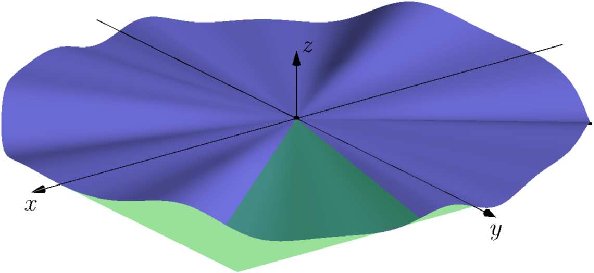
\includegraphics[width=\linewidth]{generated/asymptote/gabp1q7-2020.pdf}
\end{image}%
\tcblower
\end{figureptx}%
%
\end{enumerate}
\end{divisionexercise}%
\begin{divisionexercise}{8}{}{}{exercise-p1q82020}%
Considere uma função \(F\colon\R^2\to\R\) e as duas curvas abaixo:%
\begin{equation*}
\gamma (t) = (-5,2t ), \forall t \in \mathbb
{R}\quad \mbox {e}\quad \sigma (t) = (-5 +t,1), \forall t \in
\mathbb {R}.
\end{equation*}
Sabe-se que%
\begin{equation*}
F\big(\gamma (t)\big )= -20t^2, \forall t \in
\mathbb {R}\quad \mbox {e}\quad F\big (\sigma (t)\big )=\ln
(t^2+1)-5, \forall t \in \mathbb {R}.
\end{equation*}
%
\par
Escolha a alternativa correta para cada caso:%
\begin{enumerate}[label=\roman*]
\item{}Sobre a continuidade de \(F\) em \((-5,1)\) podemos afirmar que:%
\begin{enumerate}[label=\alph*]
\item{}é contínua em \((-5,1)\).%
\item{}não é contínua em \((-5,1)\).%
\item{}não temos informação suficiente para dizer algo.%
\end{enumerate}
%
\item{}Sobre a diferenciabilidade de \(F\) em \((-5,1)\), podemos afirmar que:%
\begin{enumerate}[label=\alph*]
\item{}é diferenciável em \((-5,1)\).%
\item{}não é diferenciável em \((-5,1)\).%
\item{}não temos informação suficiente para dizer algo.%
\end{enumerate}
%
\item{}Sobre \(\dfrac {\partial F}{\partial x} (-5,1)\) podemos afirmar que:%
\begin{enumerate}[label=\alph*]
\item{}vale \(-5\).%
\item{}vale \(0\).%
\item{}não existe.%
\item{}não é possível garantir sua existência.%
\end{enumerate}
%
\item{}Sobre \(\dfrac {\partial F}{\partial y} (-5,1)\)%
\begin{enumerate}[label=\alph*]
\item{}vale \(-10\).%
\item{}vale \(-12\).%
\item{}não existe.%
\item{}não é possível garantir sua existência.%
\end{enumerate}
%
\end{enumerate}
%
\par\smallskip%
\noindent\textbf{\blocktitlefont Resposta}.\hypertarget{answer-p1q82020-b}{}\quad{}%
\begin{multicols}{2}
\begin{enumerate}[label=\roman*]
\item{}Alternativa c.%
\item{}Alternativa c.%
\item{}Alternativa b.%
\item{}Alternativa a.%
\end{enumerate}
\end{multicols}
\par\smallskip%
\noindent\textbf{\blocktitlefont Solução}.\hypertarget{solution-p1q82020-c}{}\quad{}%
\begin{enumerate}[label=\roman*]
\item{}Apesar das curvas \(\gamma\) e \(\sigma\) serem contínuas, \(\gamma(1/2)=\sigma(0)=(-5,1)\), \(F(-5,1)=F\big(\gamma(1/2)\big)=-20(\frac{1}{2})^2=-5\), \(F\big(\sigma(0)\big)=\ln(0^2+1)-5\),%
\begin{align*}
\lim\limits_{t\to 1/2}F\big(\gamma(t)\big)&
=\lim\limits_{t\to 1/2}-20t^2=-5\text{ e}\\
\lim\limits_{t\to 0}F\big(\sigma(t)\big)&
=\lim\limits_{t\to 0}\ln(t^2+1)-5=-5,
\end{align*}
temos informações sobre \(F\) apenas ao longo de duas curvas. Poderia haver uma terceira curva ao longo da qual a função não tem o mesmo comportamento, o que mostraria sua descontinuidade ali.%
\item{}O mesmo argumento acima também se aplica aqui.%
\item{}As curvas dadas têm imagens paralelas aos eixos coordenados, ambas passando por \((-5,1)\), logo podemos usá-las para obter as derivadas parciais!%
\par
Usando as definições temos que%
\begin{align*}
\dfrac{\partial F}{\partial x}(-5,1)&
=\lim\limits_{h\to 0}\dfrac{F(-5+h,1)-F(-5,1)}{h}\\
&=\lim\limits_{h\to 0}\dfrac{F\big(\sigma(h)\big)+5}{h}=
\lim\limits_{t\to
0}\dfrac{\ln(t^2+1)}{t}=0.
\end{align*}
%
\item{}De modo totalmente análogo,%
\begin{align*}
\dfrac{\partial F}{\partial y}(-5,1)&
=\lim\limits_{k\to 0}\dfrac{F(-5,1+k)-F(-5,1)}{k}\\
&
\stackrel{(\ast)}{=}\lim\limits_{t\to
1/2}\dfrac{F\big(\gamma(t)\big)+5}{2t-1}
=\lim\limits_{t\to
1/2}\dfrac{-20t^2+5}{2t-1}=-10,
\end{align*}
onde, em \((\ast)\), fizemos a mudança \(k=2t-1\).%
\end{enumerate}
\end{divisionexercise}%
\begin{divisionexercise}{9}{}{}{exercise-p1q9-2020}%
Nesta questão \(m\) e \(k\) são números reais fixados. Considere a função \(F(x,y) = \sqrt
{1+mx^2+ky^2}\). Sabe-se que:%
\begin{itemize}[label=\textbullet]
\item{}A intersecção de \(\text {graf}(F)\) com o plano \(x=0\) está contida numa elipse no plano \(x=0\) que tem parametrização \(y(t) = 2 \cos (t)\), \(z(t) = \sin
(t)\), para todo \(t \in \mathbb {R}.\)%
\item{}A curva de nível \(c = \sqrt {2}\) de \(F\) é uma hipérbole de assíntotas \(y = \pm 2x\).%
\end{itemize}
%
\par
Com essas informações:%
\begin{enumerate}[label=\alph*]
\item{}determine \(m\) e \(k\);%
\item{}descreva o conjunto \(\text {Dom}(F)\) e faça um esboço;%
\item{}encontre uma parametrização para a parte da curva de nível que contém o ponto \((x_0,y_0) = (1,2\sqrt {2})\) e determine a reta tangente a essa curva em \((x_0,y_0)\);%
\item{}esboce o gráfico de \(F\).%
\end{enumerate}
%
\par\smallskip%
\noindent\textbf{\blocktitlefont Resposta}.\hypertarget{answer-p1q9-2020-b}{}\quad{}%
\begin{enumerate}[label=\alph*]
\item{}\(m=1\) e \(k=-\dfrac{1}{4}\).%
\item{}\(\text {Dom}(F)=\big\{(x,y)\in\mathbb R^2\colon
1+x^2-\dfrac{y^2}{4}\geq 0 \big\}\). Veja o esboço do domínio na solução.%
\item{}\(\gamma(t)=(\tan t, 2\sec(t))\), \(t\in
\big(-\dfrac{\pi}{2},\dfrac{\pi}{2}\big)\) e \(r\colon
y=\sqrt{2}x+\sqrt{2}\).%
\item{}Veja o gráfico de \(F\) na solução.%
\end{enumerate}
\par\smallskip%
\noindent\textbf{\blocktitlefont Solução}.\hypertarget{solution-p1q9-2020-c}{}\quad{}%
\begin{enumerate}[label=\alph*]
\item{}A primeira informação do enunciado nos diz que%
\begin{equation*}
z=F(0,y)=\sqrt{1+ky^2}\implies z^2-ky^2=1.
\end{equation*}
Para que isso seja descrito pela parametrização dada (uma elipse), devemos ter \(k< 0\). Além disso, tal elipse tem equação cartesiana \(z^2+\dfrac{y^2}{4}=1\). Fica fácil então ver que \(k=-\dfrac{1}{4}\).%
\par
A segunda informação nos diz que%
\begin{equation*}
F(x,y)=\sqrt{2}\implies 1+mx^2-\dfrac{y^2}{4}=2\implies
mx^2-\dfrac{y^2}{4}=1,
\end{equation*}
é uma hipérbole de assíntotas \(y=\pm 2x\).  Observe que isso garante \(m>0\), uma vez que \(k<0\). Da equação desta hipérbole, vemos que seus focos estão no eixo \(Ox\) e podemos escrever sua porção nos quadrantes \(y> 0\) como \(y=2\sqrt{mx^2-1}\), que tem como assíntotas as retas \(y=\pm 2\sqrt{m}x\). Assim, \(2\sqrt{m}=2\implies
m=1\).%
\item{}De posse dos valores de \(m\) e \(k\), temos a expressão de \(F\): \(F(x,y)=\sqrt{1+x^2-\dfrac{y^2}{4}}\). Seu domínio máximo é, então, aquele onde o termo na raiz é não-negativo, ou seja,%
\begin{equation*}
\text {Dom}(F)=\big\{(x,y)\in\mathbb R^2\colon
1+x^2-\dfrac{y^2}{4}\geq 0\big\}.
\end{equation*}
Sua representação gráfica corresponte à região entre os ramos da hipérbole \(-x^2+\dfrac{y^2}{4}=1\) (atenção aos eixos fora de escala!): \begin{figureptx}{Figura}{O domínio de \(F\) e a tangente pedida no item abaixo.}{figure-fig_gabp1q91-2020}{}%
\begin{image}{0.25}{0.5}{0.25}{}%
\resizebox{\linewidth}{!}{%
\begin{tikzpicture}
\begin{axis}[axis lines = middle,enlargelimits,
              xlabel = {$x$},
              ylabel = {$y$},
              axis on top=true]
              \addplot[name path=A, domain=-2:2, blue]
({sinh(x)},{2*cosh(x)});
\addplot[name path=B, domain=-2:2, blue]
({sinh(x)},{-2*cosh(x)});
\addplot [teal!30] fill between [of = A and B, soft
                clip={domain=-3.5:3.5}];
\addplot[domain=-2:3, olive]
{sqrt(2)*(1+x)};
              \end{axis}
\end{tikzpicture}
}%
\end{image}%
\tcblower
\end{figureptx}%
%
\item{}Como \(F(1,2\sqrt
{2})=\sqrt{1+1^2-\dfrac{(2\sqrt{2})^2}{4}}=0\), estamos falando da curva de nível \(0\) de \(F\), a qual (por pura sorte) é exatamente aquela que delimira o domínio, da qual pedimos a parte que contém o ponto dado, ou seja, vamos trabalhar com o ramo "superior" da hipérbole.%
\par
Existem muitas maneiras de parametrizar esse ramo: funções trigonométricas, trigonométricas hiperbólicas ou mesmo descrevê-la como o gráfico de uma função a uma variável:%
\begin{itemize}[label=\textbullet]
\item{}\(\gamma(t)=(\tan t, 2\sec(t))\), \(t\in
\big(-\dfrac{\pi}{2},\dfrac{\pi}{2}\big)\);%
\item{}\(\beta(t)=(\sinh t, 2\cosh t(t))\), \(t\in\R\);%
\item{}\(\alpha(t)=(t,2\sqrt{t^2+1})\), \(t\in\R\).%
\end{itemize}
%
\par
Usaremos o primeiro caso para determinar a reta tangente pedida. Para isso precisamos de \(t_0\in\big(-\dfrac{\pi}{2},\dfrac{\pi}{2}\big)\) tal que \(\gamma(t_0)=(1,2\sqrt {2})\), fácil: \(t_0=\dfrac{\pi}{4}\). A equação da reta pedida escreve-se:%
\begin{equation*}
r\colon (x,y)=\gamma(t_0)+\gamma\beta'(t_0)=(1,2\sqrt
{2})+\lambda(2,2\sqrt{2}),\lambda\in\R.
\end{equation*}
A equação geral de tal reta é \(r\colon
y=\sqrt{2}x+\sqrt{2}\).%
\item{}Pode-se perceber, fazendo \(z=F(x,y)\) que o gráfico de \(F\) satisfaz \(-x^2+\dfrac{y^2}{4}+z^2=1\), com \(z\geq 0\), ou seja, é um hiperbolóide de uma folha (seções elípticas) em torno do eixo \(Ox\). Sem isso, o gráfico da função é construído analisando-se suas curvas de nível e cortes por planos verticais. Começando pelos últimos temos:%
\begin{itemize}[label=\textbullet]
\item{}\(z=F(0,y)=\sqrt{1-\dfrac{y^2}{4}}\), uma parte de elipse;%
\item{}\(z=F(x,0)=\sqrt{1+x^2}\), um ramo de hipérbole;%
\end{itemize}
Já as curvas de nível \(c\) tem uma alteração no comportamento:%
\begin{itemize}[label=\textbullet]
\item{}\(0\leq c< 1\): hipérboles com focos no eixo \(Oy\);%
\item{}\(c=1\): par de retas concorrentes na origem, \(y=\pm 2x\);%
\item{}\(c> 1\): hipérboles com focos no eixo \(Ox\);%
\end{itemize}
%
\par
Uma figura: \begin{figureptx}{Figura}{Gráfico da função.}{figure-fig_gabp1q92-2020}{}%
\begin{image}{0.25}{0.5}{0.25}{}%
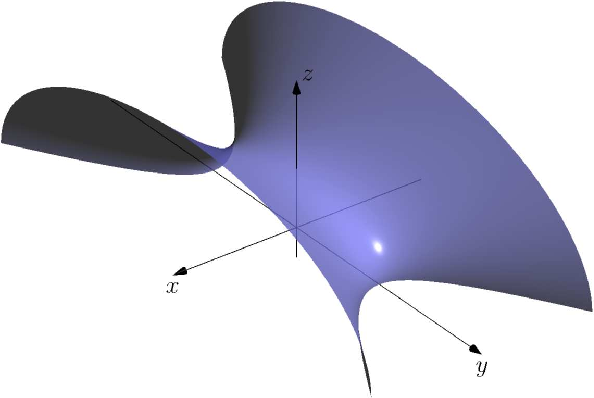
\includegraphics[width=\linewidth]{generated/asymptote/gabp1q92-2020.pdf}
\end{image}%
\tcblower
\end{figureptx}%
%
\end{enumerate}
\end{divisionexercise}%
\end{exercises-subsection-numberless}
\end{sectionptx}
\end{chapterptx}
%
%
\typeout{************************************************}
\typeout{Capítulo 6 Provas até 2019}
\typeout{************************************************}
%
\begin{chapterptx}{Capítulo}{Provas até 2019}{}{Provas até 2019}{}{}{chapter-ch_antigas}
\renewcommand*{\chaptername}{Capítulo}
\begin{introduction}{}%
Neste capítulo apresentamos um link para as soluções dos exercícios das provas aplicadas até 2019, antes da adoção do e-disciplinas como site de apoio. Naquela época o site era construído em HTML pelo coordenador da disciplinas e este ainda não conhecia o \href{https://pretextbook.org}{PreTeXt}\footnote{\nolinkurl{pretextbook.org}\label{fn-ch_antigas-b-a-b}}. Aos poucos migraremos aquelas soluções para este formato.%
\par
Acesse as provas até 2019 \href{https://www.ime.usp.br/\~lymber/teaching/2019/2019-2454/material.html}{aqui}\footnote{\nolinkurl{ime.usp.br/\~lymber/teaching/2019/2019-2454/material.html}\label{fn-ch_antigas-b-b-b}}.%
\end{introduction}%
\end{chapterptx}
%
\appendix%
%
\clearpage\phantomsection%
\addcontentsline{toc}{part}{Apêndices}%
%
%
\typeout{************************************************}
\typeout{Apêndice A Principais Resultados}
\typeout{************************************************}
%
\begin{appendixptx}{Apêndice}{Principais Resultados}{}{Principais Resultados}{}{}{appendix-apendice}
\renewcommand*{\appendixname}{Apêndice}
\begin{introduction}{}%
Nas sessões abaixo listamos, quase sempre sem demonstração, alguns dos principais resultados teóricos e definições utilizados na resolução dos exercícios selecionados.%
\par
É um material para referência rápida. Os detalhes devem ser preenchidos com a leitura da bibliografia recomendada em cada curso.%
\end{introduction}%
%
%
\typeout{************************************************}
\typeout{Seção A.1 Cálculo 1}
\typeout{************************************************}
%
\begin{sectionptx}{Seção}{Cálculo 1}{}{Cálculo 1}{}{}{section-ap_calc1}
\begin{theorem}{Teorema}{(Cauchy).}{}{theorem-teo_cauchy}%
Sejam \(f,g\colon [a,b]\to\R\) duas funções contínuas, que são deriváveis em \((a,b)\). Então existe \(c\in (a,b)\) tal que%
\begin{equation*}
\big(f(b)-f(a)\big)g'(c)=\big(g(b)-g(a)\big)f'(c)
\end{equation*}
%
\begin{remark}{Nota}{}{remark-teo_cauchy-d}%
Este teorema é uma generalização do Teorema do Valor Médio, o qual é obtido fazendo \(g(x)=x\).\end{remark}
\end{theorem}
\begin{proof}{Demonstração}{}{proof-teo_cauchy-c}
Vamos construir uma função e aplicar a ela o \href{https://pt.wikipedia.org/wiki/Teorema_de_Rolle}{Teorema de Rolle}\footnotemark{}. Consideremos então \(h\colon [a,b]\to\R\) dada por%
\begin{equation*}
h(x)=\big(f(b)-f(a)\big)g(x)-\big(g(b)-g(a)\big)f(x).
\end{equation*}
Esta função é contínua em \([a,b]\) e derivável em \((a,b)\). Cálculos diretos mostram que \(h(b)=g(a)f(b)-g(b)f(a)=h(a)\). Segue, do Teorema de Rolle, que existe \(c\in (a,b)\) tal que \(h'(c)=0\), ou seja,%
\begin{equation*}
\big(f(b)-f(a)\big)g'(c)-\big(g(b)-g(a)\big)f'(c)=0.\qedhere
\end{equation*}
%
\end{proof}
\footnotetext[1]{\nolinkurl{https://pt.wikipedia.org/wiki/Teorema_de_Rolle}\label{fn-teo_cauchy-c-a-b}}%
\begin{theorem}{Teorema}{(Fermat).}{}{theorem-teo_fermat}%
Seja \(f\colon ]a,b[\to\R\) derivável em \(x_0\in
]a,b[\). Se \(x_0\) é um ponto de máximo ou mínimo local de \(f\), então \(f'(x_0)=0\).%
\begin{remark}{Nota}{}{remark-teo_fermat-d}%
O teorema não vale se o domínio de \(f\) é um intervalo fechado: \(f(x)=x\), \(x\in [0,1]\), não tem derivada nula em nenhum ponto e assume valores máximo e mínimo (nos extremos do intervalo).%
\par
O teorema não admite recíproca, ou seja, se \(f'(x_0)=0\) não podemos dizer que \(x_0\) é ponto de máximo ou mínimo local de \(f\): \(f(x)=x^3\), \(x\in ]-1,1[\), é tal que \(f'(0)=0\), mas \(x_0=0\) não é máximo nem mínimo local de \(f\).%
\end{remark}
\end{theorem}
\begin{proof}{Demonstração}{}{proof-teo_fermat-c}
Lembramos que \(f\) é derivável em \(x_0\), se existe \(\rho\colon ]a,b[\to\R\) contínua em \(x_0\), tal que%
\begin{equation}
f(x)=f(x_0)+(x-x_0)\rho(x),\label{men-eq_fermat}
\end{equation}
e, nesse caso, temos \(\rho(x_0)=f'(x_0)\).%
\par
Suponha que \(x_0\) é um ponto de máximo local de \(f\). O caso de mínimo local é análogo e um excelente exercício para testar sua compreensão da demonstração. Consideremos duas situações:%
\begin{itemize}[label=\textbullet]
\item{}\(f'(x_0)>0\): nesse caso, \(\rho(x_0)>0\) e, da continuidade de \(\rho\), temos que \(\rho(x)>0\) para todo \(x\in I\), onde \(I\) é um intervalo aberto centrado em \(x_0\) e inteiramente contido em \(]a,b[\). Se \(x\in
I\), \(x>x_0\), então a equação \hyperref[men-eq_fermat]{({\xreffont\ref{men-eq_fermat}})} nos diz que%
\begin{equation*}
f(x)=f(x_0)+(x-x_0)\rho(x)>f(x_0),
\end{equation*}
contradizendo o fato de \(x_0\) ser máximo local.%
\item{}\(f'(x_0)<0\): agora, \(\rho(x_0)<0\) e, como antes, \(\rho(x)<0\) para todo \(x\in I\), onde \(I\) é um intervalo como o do caso anterior. Se \(x\in I\), \(x<x_0\), então a equação \hyperref[men-eq_fermat]{({\xreffont\ref{men-eq_fermat}})} nos diz que%
\begin{equation*}
f(x)=f(x_0)+(x-x_0)\rho(x)>f(x_0),
\end{equation*}
contradizendo o fato de \(x_0\) ser máximo local.%
\end{itemize}
Com isso, só é possível \(f'(x_0)=0\).%
\end{proof}
\end{sectionptx}
%
%
\typeout{************************************************}
\typeout{Seção A.2 Curvas de Nível}
\typeout{************************************************}
%
\begin{sectionptx}{Seção}{Curvas de Nível}{}{Curvas de Nível}{}{}{section-ap_func}
\begin{definition}{Definição}{}{definition-curva_nivel}%
Sejam \(f\colon A\subseteq\R^2\to\R\) e \(c\in\R\). A \terminology{curva de nível} ou \terminology{conjunto de nível} do nível \(c\) de \(f\) é o conjunto%
\begin{equation*}
f^{-1}(c)=\{(x,y)\in
A\colon f(x,y)=c\},
\end{equation*}
\end{definition}
A curva de nível \(c\) é, em outras palavras, o conjunto de todos os pontos no domínio de \(f\), onde esta vale \(c\).%
\begin{example}{Exemplo}{}{example-ap_func-d}%
Determine as curvas nível da função \(f\colon\R^2\to\R\) dada por \(f(x,y)=x^2+y^2\).%
\par\smallskip%
\noindent\textbf{\blocktitlefont Solução}.\hypertarget{solution-ap_func-d-b}{}\quad{}Começamos observando que o domínio de \(f\) é todo o \(\R^2\) e sua imagem é o conjunto dos reais não-negativos, indicado por \(\R_{\geq 0}\). Isto posto notamos que, para todo \(c<0\), temos \(f^{-1}(c)=\emptyset\). Vejamos o que acontece com \(c\geq0\):%
\begin{itemize}[label=\textbullet]
\item{}\(c=0\): \(f(x,y)=0\iff x^2+y^2=0\iff
(x,y)=(0,0)\);%
\item{}\(c>0\): \(f(x,y)=c\iff x^2+y^2=c\). Neste caso, as soluções são exatamente pontos da circunferência de raio \(\sqrt{c}\), centrada na origem.%
\end{itemize}
\begin{sidebyside}{2}{0.05}{0.05}{0.1}%
\begin{sbspanel}{0.4}[center]%
\begin{panelfigureptx}{Figura}{Curvas de nível.}{figure-fig_parabeli}{}%
\resizebox{\linewidth}{!}{%
\begin{tikzpicture}
\draw[->] (-3,0) -- (3,0) node[below] {$x$};
\draw[->] (0,-3) -- (0,3) node[right] {$y$};
\draw[orange] (0,0) circle (1pt);
\foreach \i in {1,2,3,4} {\draw[orange] (0,0) circle (\i/2);};
\end{tikzpicture}
}%
\tcblower
\end{panelfigureptx}%
\end{sbspanel}%
\begin{sbspanel}{0.4}[center]%
\begin{panelfigureptx}{Figura}{Gráfico de função e cortes de nível}{figure-fig_parabeli3d}{}%
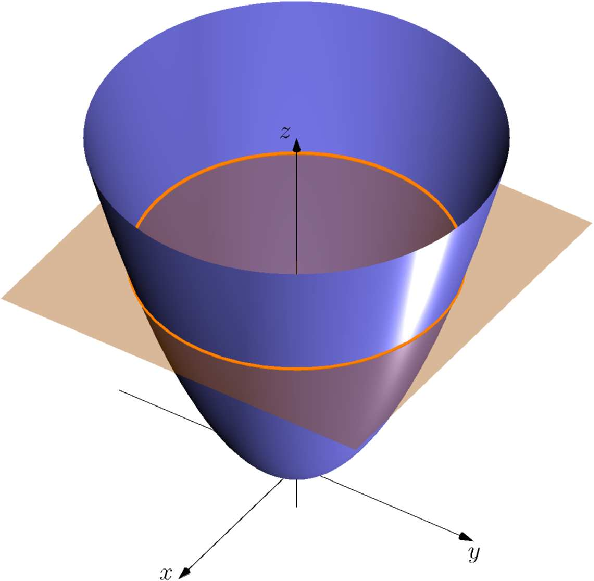
\includegraphics[width=\linewidth]{generated/asymptote/fig_parabeli-graf.pdf}
\tcblower
\end{panelfigureptx}%
\end{sbspanel}%
\end{sidebyside}%
%
\end{example}
\begin{example}{Exemplo}{}{example-ap_func-e}%
Determine as curvas nível da função \(f\colon\R^2\to\R\) dada por \(f(x,y)=y^2-x^2\).%
\par\smallskip%
\noindent\textbf{\blocktitlefont Solução}.\hypertarget{solution-ap_func-e-b}{}\quad{}Começamos observando que o domínio de \(f\) é todo o \(\R^2\) e sua imagem é o conjunto de todos os reais. Vejamos o que acontece com \(c\in\R\):%
\begin{itemize}[label=\textbullet]
\item{}\(c<0\): \(f(x,y)=c\iff y^2-x^2=c\iff\), que descreve uma hipérbole com focos no eixo \(Ox\);%
\item{}\(c=0\): \(f(x,y)=0\iff y^2-x^2=0\), que descreve o par de retas concorrentes \(y=x\) e \(y=-x\).%
\item{}\(c>0\): \(f(x,y)=c\iff y^2-x^2=c\iff\), que descreve uma hipérbole com focos no eixo \(Oy\);%
\end{itemize}
\begin{sidebyside}{2}{0.05}{0.05}{0.1}%
\begin{sbspanel}{0.4}[center]%
\begin{panelfigureptx}{Figura}{Curvas de nível.}{figure-fig_parabhip}{}%
\resizebox{\linewidth}{!}{%
\begin{tikzpicture}
\draw[->] (-3,0) -- (3,0) node[below] {$x$};
\draw[->] (0,-3) -- (0,3) node[right] {$y$};
\draw[orange] (-3,3) -- (3,-3);
\draw[orange] (-3,-3) -- (3,3);
\draw[green,variable=\t,domain=-1.75:1.75,samples=100]
plot ({sinh(\t)},{cosh(\t)});
\draw[green,variable=\t,domain=-1.75:1.75,samples=100]
plot ({sinh(\t)},{-cosh(\t)});
\draw[red,variable=\t,domain=-1.75:1.75,samples=100]
plot ({cosh(\t)},{sinh(\t)});
\draw[red,variable=\t,domain=-1.75:1.75,samples=100]
plot ({-cosh(\t)},{sinh(\t)});
\end{tikzpicture}
}%
\tcblower
\end{panelfigureptx}%
\end{sbspanel}%
\begin{sbspanel}{0.4}[center]%
\begin{panelfigureptx}{Figura}{Gráfico de função e cortes de nível}{figure-fig_parabhip3d}{}%
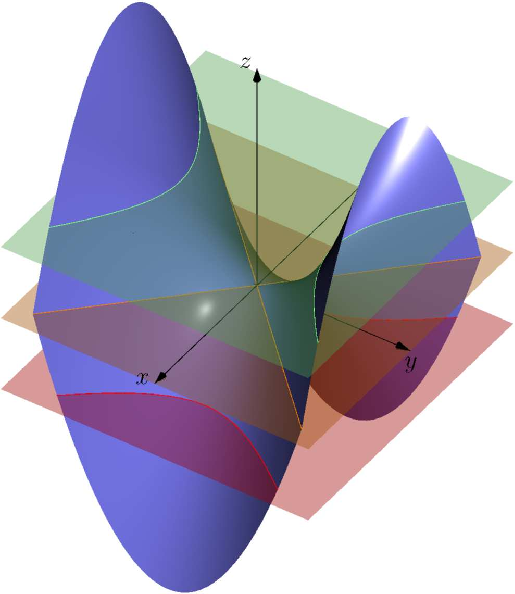
\includegraphics[width=\linewidth]{generated/asymptote/fig_parabhip-graf.pdf}
\tcblower
\end{panelfigureptx}%
\end{sbspanel}%
\end{sidebyside}%
%
\end{example}
\begin{example}{Exemplo}{}{example-ap_func-f}%
Determine as curvas nível da função \(f\colon\R^2\to\R\) dada por \(f(x,y)=\dfrac{x^2}{x^2-y^2}\).%
\par\smallskip%
\noindent\textbf{\blocktitlefont Solução}.\hypertarget{solution-ap_func-f-b}{}\quad{}Aqui o domínio da função é o conjunto%
\begin{equation*}
D_f=\big\{(x,y\in\R^2\colon x^2\neq y^2\big\}.
\end{equation*}
Isto significa obviamente, mas nunca é demais alertar que, os pontos das bissetrizes dos quadrantes não podem estar em nenhuma curva de nível da função deste exemplo. Com isso em mente temos que equação que define cada curva de nível é%
\begin{equation}
\dfrac{x^2}{x^2-y^2}=c \iff (1-c)x^2+cy^2=0, y\neq\pm x.\label{men-niv_exemplo}
\end{equation}
%
\par
Separando em casos:%
\begin{itemize}[label=\textbullet]
\item{}\(c=1\): A queação torna-se \(y^2=0\iff y=0\), que é o eixo \(Ox\), exceto a origem (restrição no domínio);%
\item{}\(c=0\): A queação torna-se \(x^2=0\iff x=0\), que é o eixo \(Oy\), novamente excluindo-se a origem;%
\item{}\(0<c<1\): os coeficiente de \(x^2\) e \(y^2\) são ambos positivos na equação \hyperref[men-niv_exemplo]{({\xreffont\ref{men-niv_exemplo}})}, donde a única solução seria \((0,0)\), que não pertence a \(D_f\), isso mostra que a função não assume valores entre \(0\) e \(1\);%
\item{}Para os demais valores de \(c\), \(c< 0\) ou \(c>1\), as soluções são retas concorrentes, exceto a origem.%
\end{itemize}
%
\par
\begin{sidebyside}{2}{0.05}{0.05}{0.1}%
\begin{sbspanel}{0.4}[center]%
\begin{panelfigureptx}{Figura}{Curvas de nível.}{figure-fig_exemplo}{}%
\resizebox{\linewidth}{!}{%
\begin{tikzpicture}
\draw[->] (-3,0) -- (3,0) node[below] {$x$};
\draw[->] (0,-3) -- (0,3) node[right] {$y$};
\draw[dashed] (-3,3) -- (3,-3);
\draw[dashed] (-3,-3) -- (3,3);
\draw (0,0) circle (2pt);
\foreach \a in {55,65,...,125} {
\draw[red] ({2pt*cos(\a)},{2pt*sin(\a)}) -- ({3*cos(\a)},{3*sin(\a)});};
\foreach \a in {235,245,...,305} {
\draw[red] ({2pt*cos(\a)},{2pt*sin(\a)}) --
({3*cos(\a)},{3*sin(\a)});};
\foreach \a in {-35,-25,...,35} {
\draw[orange] ({2pt*cos(\a)},{2pt*sin(\a)}) -- ({3*cos(\a)},{3*sin(\a)});};
\foreach \a in {145,155,...,215} {
\draw[orange] ({2pt*cos(\a)},{2pt*sin(\a)}) -- ({3*cos(\a)},{3*sin(\a)});};
\end{tikzpicture}
}%
\tcblower
\end{panelfigureptx}%
\end{sbspanel}%
\begin{sbspanel}{0.4}[center]%
\begin{panelfigureptx}{Figura}{Gráfico de função e cortes de nível}{figure-fig_exemplo-nivel3d}{}%
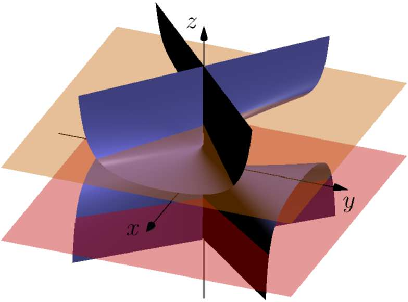
\includegraphics[width=\linewidth]{generated/asymptote/fig_exemplonivel-graf.pdf}
\tcblower
\end{panelfigureptx}%
\end{sbspanel}%
\end{sidebyside}%
%
\end{example}
\end{sectionptx}
%
%
\typeout{************************************************}
\typeout{Seção A.3 Cálculo de Limites}
\typeout{************************************************}
%
\begin{sectionptx}{Seção}{Cálculo de Limites}{}{Cálculo de Limites}{}{}{section-ap_limcont}
\begin{introduction}{}%
Apresentamos a seguir os principais resultados para o cálculo de limites. Ao final apresentamos a conexão entre o cálculo de limites e continuidade num ponto.%
\end{introduction}%
\begin{proposition}{Proposição}{(Limite da composta).}{}{proposition-prop_comp}%
Sejam \(f\colon I\subseteq\R\to\R\), contínua em \(L\in
I\) e \(g\colon A\subseteq\R^r\to\R\), tal que \(\lim\limits_{(x,y)\to(x_0,y_0)} g(x,y)=L\). Então%
\begin{equation*}
\lim\limits_{(x,y)\to(x_0,y_0)}f\big(g(x,y)\big)=f\Big(\lim\limits_{(x,y)\to(x_0,y_0)}g(x,y)\Big)=f(L)\text{.}
\end{equation*}
%
\begin{remark}{Nota}{}{remark-prop_comp-d}%
Este é o resultado que permite "passar o limite para dentro" de uma função contínua.\end{remark}
\end{proposition}
\begin{proof}{Demonstração}{}{proof-prop_comp-c}
Junte os ingredientes:%
\begin{enumerate}
\item{}\(f\) contínua em \(L\in I\) diz que, dado \(\epsilon>0\), existe \(\delta_1>0\) tal que%
\begin{equation}
|x-L|<\delta_1\implies
|f(x)-f(L)|<\epsilon.\label{men-limcomp1}
\end{equation}
\(\lim\limits_{(x,y)\to(x_0,y_0)} g(x,y)=L\) diz que, dado \(\epsilon_2>0\), existe \(\delta_2>0\) tal que%
\begin{equation}
0<\|(x,y)-(x_0,y_0)\|<\delta_2 \implies
|g(x,y)-L|<\epsilon_2.\label{men-limcomp2}
\end{equation}
%
\end{enumerate}
%
\par
Dado \(\epsilon>0\), aplicando \(\delta_1\) dado por \hyperref[men-limcomp1]{({\xreffont\ref{men-limcomp1}})} como \(\epsilon_2\) em \hyperref[men-limcomp2]{({\xreffont\ref{men-limcomp2}})} temos que%
\begin{equation*}
0<\|(x,y)-(x_0,y_0)\|<\delta_2 \implies
|g(x,y)-L|<\delta_1\implies |f(x)-f(L)|<\epsilon,
\end{equation*}
ou seja, \(\lim\limits_{(x,y)\to(x_0,y_0)}f\big(g(x,y)\big)=f(L)\).%
\end{proof}
\begin{example}{Exemplo}{}{example-exemplo_comp}%
Calcule, caso exista, \(\lim\limits_{(x,y)\to(0,0)}\dfrac{\sin(x^2+y^2)}{x^2+y^2}\).%
\par\smallskip%
\noindent\textbf{\blocktitlefont Solução}.\hypertarget{solution-exemplo_comp-b}{}\quad{}Considere \(f(t)=\begin{cases} \dfrac{\sin t}{t},& t\neq 0\\
\hfill 1,& t=0\end{cases}\) e \(g(x,y)=x^2+y^2\). Claramente, para todo \((x,y)\neq
(0,0)\), \(\dfrac{\sin(x^2+y^2)}{x^2+y^2}=f\big(g(x,y)\big)\). Como \(f\) é contínua em \(t=0\) (limite trigonométrico fundamental) e \(\lim\limits_{(x,y)\to(0,0)}g(x,y)=0\), temos%
\begin{equation*}
\lim\limits_{(x,y)\to(0,0)}\dfrac{\sin(x^2+y^2)}{x^2+y^2}=\lim\limits_{(x,y)\to(0,0)}f\big(g(x,y)\big)=f\Big(\lim\limits_{(x,y)\to(0,0)}g(x,y)\Big)=f(0)=1.
\end{equation*}
\end{example}
\begin{theorem}{Teorema}{(Confronto).}{}{theorem-teo_confronto}%
Sejam \(f,g,h\colon A\subseteq\R^2\to\R\) funções tais que \(g(x,y)\leq f(x,y)\leq h(x,y)\) para todo \((x,y)\in
A\). Se \(\lim\limits_{(x,y)\to(x_0,y_0)}
g(x,y)=\lim\limits_{(x,y)\to(x_0,y_0)} h(x,y)=L\in\R\), então \(\lim\limits_{(x,y)\to(x_0,y_0)} f(x,y)=L\).%
\end{theorem}
\begin{proof}{Demonstração}{}{proof-teo_confronto-c}
Basta escrever a definição de limite:%
\par
\(\lim\limits_{(x,y)\to(x_0,y_0)}
g(x,y)=L\in\R\) significa que dado \(\epsilon>0\), existe \(\delta_1>0\) tal que%
\begin{equation*}
0<\|(x,y)-(x_0,y_0)\|<\delta_1 \implies
|g(x,y)-L|<\epsilon
\end{equation*}
e \(\lim\limits_{(x,y)\to(x_0,y_0)}
h(x,y)=L\in\R\) significa que dado \(\epsilon>0\), existe \(\delta_2>0\) tal que%
\begin{equation*}
0<\|(x,y)-(x_0,y_0)\|<\delta_2 \implies
|h(x,y)-L|<\epsilon\text{.}
\end{equation*}
%
\par
Para cada \(\epsilon>0\), tome \(\delta=\min\{\delta_1,\delta_2\}\). Para todo \((x,y)\in\R^2\) tal que \(\|(x,y)-(x_0,y_0)\|< \delta\), "abrindo os módulos" e usando as desigualdades da hipótese, temos que%
\begin{equation*}
-\epsilon<g(x,y)-L<f(x,y)-L<h(x,y)-L<\epsilon\implies
|f(x,y)-L|<\epsilon\text{,}
\end{equation*}
ou seja, \(\lim\limits_{(x,y)\to(x_0,y_0)} f(x,y)=L\).%
\end{proof}
\begin{definition}{Definição}{(Função Limitada).}{definition-def_limitada}%
Uma função \(f\colon A\subseteq\R^2\to\R\) é \terminology{limitada}, se existe \(M\in\R\) tal que \(|f(x,y)|< M\), para todo \((x,y)\in A\).%
\end{definition}
Veja alguns exemplos de funções limitadas no vídeo abaixo.%
\begin{figureptx}{Figura}{Funções limitadas (até 10m30s).}{figure-vid_limitada}{}%
\begin{sidebyside}{2}{0.075}{0.075}{0.17}%
\begin{sbspanel}{0.47}%
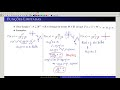
\includegraphics[width=\linewidth]{generated/youtube/video-2.jpg}
\end{sbspanel}%
\begin{sbspanel}{0.21}%

\includegraphics[width=\linewidth]{generated/qrcode/video-2.png}
\end{sbspanel}%
\end{sidebyside}%
\tcblower
\end{figureptx}%
\begin{corollary}{Corolário}{(Limitada \(\times\) Tende a zero).}{}{corollary-cor_confronto}%
Sejam \(f,g\colon A\subseteq\R^2\to\R\) funções tais que \(f\) é limitada e \(\lim\limits_{(x,y)\to(x_0,y_0)}
g(x,y)=0\). Então \(\lim\limits_{(x,y)\to(x_0,y_0)}
f(x,y)\, g(x,y)=0\).%
\end{corollary}
\begin{proof}{Demonstração}{}{proof-cor_confronto-c}
Como \(f\) é limitada, existe \(M> 0\) tal que \(|f(x,y)|< M\). Multiplicando por \(|g(x,y)|\), temos \(|f(x,y)\, g(x,y)|< M|g(x,y)|\), ou seja,%
\begin{equation*}
-M|g(x,y)|< f(x,y)\, g(x,y)< M|g(x,y)|\text{.}
\end{equation*}
Usando a \hyperref[proposition-prop_comp]{Proposição~{\xreffont\ref{proposition-prop_comp}}}, temos que \(\lim\limits_{(x,y)\to(x_0,y_0)} \pm M|g(x,y)|=\pm
M|\lim\limits_{(x,y)\to(x_0,y_0)} g(x,y)|=0\). Logo, \(\lim\limits_{(x,y)\to(x_0,y_0)} f(x,y)\, g(x,y)=0\).%
\end{proof}
\begin{theorem}{Teorema}{}{}{theorem-teo_limcurvas}%
Sejam \(f\colon A\subseteq\R^2\to\R\) uma função tal que \(\lim\limits_{(x,y)\to(x_0,y_0)} f(x,y)=L\in\R\) e \(\gamma\colon I\subseteq\R\to\R^2\) uma curva contínua tal que \(\lim\limits_{t\to t_0}\gamma(t)=(x_0,y_0)\). Então \(\lim\limits_{t\to t_0} f\big(\gamma(t)\big)=L\).%
\begin{remark}{Nota}{}{remark-teo_limcurvas-c}%
Este teorema é bem mais interessante na contra-positiva: se existem duas curvas \(\gamma_1\) e \(\gamma_2\) nas condições do enunciado tais que %
\begin{itemize}[label=\textbullet]
\item{}\(\lim\limits_{t\to t_0}
f\big(\gamma_1(t)\big)\neq\lim\limits_{t\to t_0}
f\big(\gamma_2(t)\big)\), ou%
\item{}\(\lim\limits_{t\to t_0}
f\big(\gamma_1(t)\big)\) não existe%
\end{itemize}
 então \(\lim\limits_{(x,y)\to(x_0,y_0)} f(x,y)\) não existe.\end{remark}
\end{theorem}
\begin{proof}{Demonstração}{}{proof-teo_limcurvas-b}
Mais uma vez, junte os ingredientes:%
\begin{enumerate}
\item{}\(\lim\limits_{(x,y)\to(x_0,y_0)} f(x,y)=L\) diz que, dado \(\epsilon>0\), existe \(\delta_1>0\) tal que%
\begin{equation}
0<\|(x,y)-(x_0,y_0)\|<\delta_1\implies
|f(x,y)-L|<\epsilon.\label{men-limcomp3}
\end{equation}
%
\item{}\(\lim\limits_{t\to t_0} \gamma(t)=(x_0,y_0)\) diz que, dado \(\epsilon_2>0\), existe \(\delta_2>0\) tal que%
\begin{equation}
0<|t-t_0|<\delta_2\implies
\|\gamma(t)-(x_0,y_0)\|<\epsilon_2.\label{men-limcomp4}
\end{equation}
%
\end{enumerate}
%
\par
Como antes, dado \(\epsilon>0\), use \(\delta_1\) dado em \hyperref[men-limcomp3]{({\xreffont\ref{men-limcomp3}})} como \(\epsilon_2\) em \hyperref[men-limcomp4]{({\xreffont\ref{men-limcomp4}})} e então%
\begin{equation*}
0<|t-t_0|<\delta_2\implies \|\gamma(t)-(x_0,y_0)\|<
\delta_1\implies |f\big(\gamma(t)\big)-L|<\epsilon,
\end{equation*}
ou seja, \(\lim\limits_{t\to t_0} f\big(\gamma(t)\big)=L\).%
\end{proof}
\begin{theorem}{Teorema}{(Limite e Continuidade).}{}{theorem-teo_limcont}%
Sejam \(f\colon A\subseteq\R^2\to\R\) uma função e \((x_0,y_0)\in A\). Então \(f\) é contínua em \((x_0,y_0)\) se, e somente se,%
\begin{equation*}
\lim\limits_{(x,y)\to(x_0,y_0)} f(x,y)=f(x_0,y_0).
\end{equation*}
%
\end{theorem}
\begin{proof}{Demonstração}{}{proof-teo_limcont-c}
É realmente uma consequência direta das definições de limite e continuidade.%
\end{proof}
\end{sectionptx}
%
%
\typeout{************************************************}
\typeout{Seção A.4 Derivadas Parciais e Diferenciabilidade}
\typeout{************************************************}
%
\begin{sectionptx}{Seção}{Derivadas Parciais e Diferenciabilidade}{}{Derivadas Parciais e Diferenciabilidade}{}{}{section-ap_diff}
\begin{introduction}{}%
Apresentamos a seguir as principais definições e resultados sobre derivadas parciais, diferenciabilidade e plano tangente ao gráfico de uma função, sempre ilustrados com exemplos e contra-exemplos.%
\end{introduction}%
\begin{definition}{Definição}{(Derivadas parciais).}{definition-def_derpar}%
Sejam \(f\colon A\subseteq\R^2\to\R\) uma função e \((x_0,y_0)\) um ponto no \href{https://pt.wikipedia.org/wiki/Interior_(topologia)}{interior}\footnotemark{} de \(A\). As \terminology{derivadas parciais} de \(f\) em \((x_0,y_0)\) são dadas por%
\begin{align*}
\dfrac{\partial f}{\partial x}(x_0,y_0)
&=\lim\limits_{h\to
0}\dfrac{f(x_0+h,y_0)-f(x_0,y_0)}{h};\\
\dfrac{\partial f}{\partial y}(x_0,y_0)
&=\lim\limits_{k\to
0}\dfrac{f(x_0,y_0+k)-f(x_0,y_0)}{k}.
\end{align*}
%
\par
É frequente na literatura encontrar \(f_x(x_0,y_0)\) indicando \(\dfrac{\partial f}{\partial x}(x_0,y_0)\) e \(f_y(x_0,y_0)\) no lugar de \(\dfrac{\partial f}{\partial
y}(x_0,y_0)\).%
\end{definition}
\footnotetext[1]{\nolinkurl{https://pt.wikipedia.org/wiki/Interior_(topologia)}\label{fn-def_derpar-b-a-d}}%
\begin{remark}{Nota}{}{remark-obs_apintderpar}%
Na definição acima apenas uma das coordenadas varia, o que se generalizaria para derivadas parciais de funções com mais de duas variáveis. Veja abaixo uma figura que dá a interpretação geométrica das derivadas parciais num ponto. \begin{figureptx}{Figura}{Interpretação das derivadas parciais}{figure-fig_apderpar}{}%
\begin{image}{0.25}{0.5}{0.25}{}%
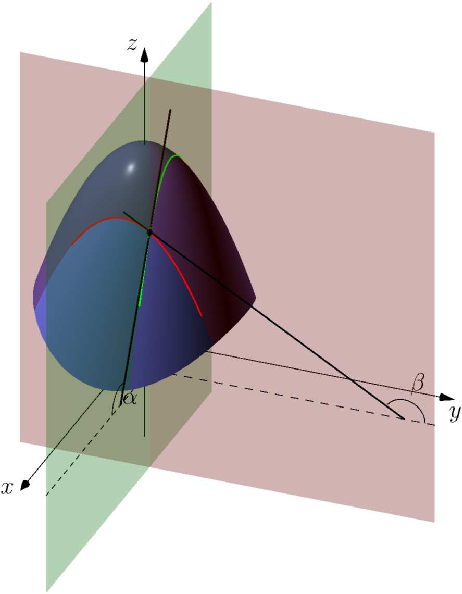
\includegraphics[width=\linewidth]{generated/asymptote/apderpar.pdf}
\end{image}%
\tcblower
\end{figureptx}%
%
\par
Assim, \(\dfrac{\partial f}{\partial x}(x_0,y_0)=\tan \alpha\) e \(\dfrac{\partial f}{\partial y}(x_0,y_0)=\tan \beta\).%
\par
Fixando uma das variáveis de \(f\), digamos \(y=y_0\) (pense nela como uma constante real), temos a função de uma variável \(g(x)=f(x,y_0)\). Se \(g\) derivável em \(x_0\), então \(f_x(x_0,y_0)=g'(x_0)\). Analogamente, se \(h(y)=f(x_0,y)\) é derivável em \(y_0\), então \(f_y(x_0,y_0)=h'(y_0)\).%
\end{remark}
\begin{remark}{Nota}{}{remark-ap_diff-e}%
Aqui aparece uma primeira diferença em relação ao cálculo em uma variável: lá toda função derivável num ponto é automaticamente contínua nesse ponto; aqui a existência das derivadas parciais em \((x_0,y_0)\) não garante a continuidade da função em \((x_0,y_0)\). Veja um exemplo a seguir.\end{remark}
\begin{example}{Exemplo}{}{example-exemplo_parcont}%
A função \(f(x,y)=\begin{cases}
\dfrac{xy}{x^2+y^2},&(x,y)\neq (0,0);\\
\hfill 0,& (x,y)=(0,0)\end{cases}\) admite derivadas parciais em \((0,0)\), mas não é contínua em \((0,0)\).%
\par
Precisamos calcular as derivadas parciais pela definição, já que a regras de derivação do quociente não se aplica (denominador se anula no ponto estudado). Então%
\begin{align*}
\dfrac{\partial f}{\partial x}(0,0)
&=\lim\limits_{h\to 0}\dfrac{f(0+h,0)-f(0,0)}{h}
=\lim\limits_{h\to 0}\dfrac{\dfrac{h\cdot 0}{h^2+0^2}-0}{h}
=0;\\
\dfrac{\partial f}{\partial y}(0,0)
&=\lim\limits_{k\to 0}\dfrac{f(0,0+k)-f(0,0)}{k}
=\lim\limits_{k\to 0}\dfrac{\dfrac{0\cdot k}{0^2+k^2}-0}{k}
=0,
\end{align*}
o que era de se esperar, uma vez que \(f\) é constante (nula) ao longo dos eixos coordenados.%
\par
Porém, ao longo da curva \(\gamma(t)=(t,t)\), temos%
\begin{equation*}
\lim\limits_{t\to 0}f\big(\gamma(t)\big)=\lim\limits_{t\to 0}
\dfrac{t^2}{2t^2}=\dfrac{1}{2}\neq 0=f(0,0),
\end{equation*}
mostrando, de acordo com o \hyperref[theorem-teo_limcurvas]{Teorema~{\xreffont\ref{theorem-teo_limcurvas}}}, que \(f\) não é contínua em \((0,0)\).%
\par
Veja o gráfico de \(f\) e verifique que o comportamento ao longo dos eixos \(Ox\) e \(Oy\) não dertermina o que acontece em outras direções no domínio. \begin{figureptx}{Figura}{Gráfico de função e cortes de nível}{figure-fig_apdercont}{}%
\begin{image}{0.25}{0.5}{0.25}{}%
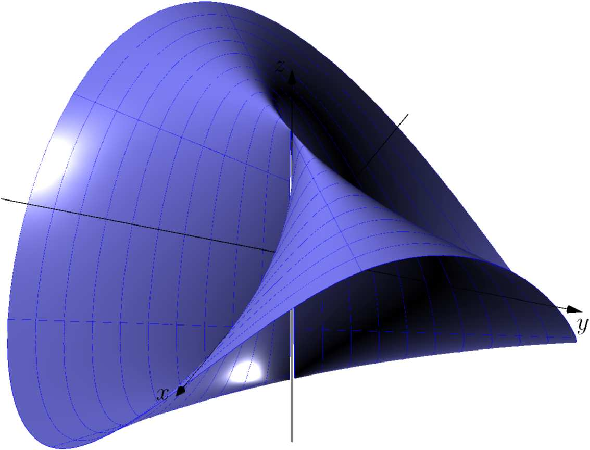
\includegraphics[width=\linewidth]{generated/asymptote/dercont.pdf}
\end{image}%
\tcblower
\end{figureptx}%
%
\end{example}
Isto mostra que precisamos de algo "mais forte" do que exigir apenas a existência de derivadas parciais sequeremos aproximar a função por algo linear numa vizinhança de um ponto, independentemente como nos aproximamos desse ponto (e não apenas paralelamente aos eixos coordenados, como ocorre nas derivadas parciais).%
\begin{definition}{Definição}{(Diferenciabilidade e Plano Tangente).}{definition-def_diff}%
Sejam \(f\colon A\subseteq\R^2\to\R\) uma função e \((x_0,y_0)\) um ponto no interior de \(A\). A função \(f\) é \terminology{diferenciável} em \((x_0,y_0)\) se%
\begin{equation*}
\lim\limits_{(h,k)\to(0,0)}
\dfrac{f(x_0+h,y_0+k)-f(x_0,y_0)-f_x(x_0,y_0)h-f_y(x_0,y_0)k}
{\sqrt{h^2+k^2}}=0.
\end{equation*}
%
\par
Se \(f\) é diferenciável em \((x_0,y_0)\), o \terminology{plano tangente} ao seu gráfico no ponto \(\big(x_0,y_0,f(x_0,y_0)\big)\) tem equação%
\begin{equation*}
\pi\colon
f_x(x_0,y_0)(x-x_0)+f_y(x_0,y_0)(y-y_0)-z+f(x_0,y_0)=0.
\end{equation*}
%
\end{definition}
Com isso, o \terminology{vetor normal} ao gráfico nesse pontos é%
\begin{equation*}
n_f(x_0,y_0)=\big(f_x(x_0,y_0),f_y(x_0,y_0),-1\big),
\end{equation*}
e a equação da \terminology{reta normal} naquele ponto é%
\begin{equation*}
r\colon (x,yz)=\big(x_0,y_0,f(x_0,y_0)\big)+\lambda
n_f(x_0,y_0),\quad\\lambda\in\R.
\end{equation*}
%
\begin{remark}{Nota}{}{remark-ap_diff-j}%
A equação do plano tangente pode ser reescrita como uma função afim%
\begin{equation*}
z(x,y)=f_x(x_0,y_0)(x-x_0)+f_y(x_0,y_0)(y-y_0). 
\end{equation*}
Com isso, de maneira intuitiva, a definição de diferenciabilidade diz que a diferença entre o valor de \(f(x_0+h,y_0+k)\) e a sua estimativa por \(z(x_0+h,y_0+k)\) tende a zero "mais rapidamente" que a distância entre \((x_0+h,y_0+k)\) e \((x_0,y_0)\). Isto é exatamente o que acontece para funções deriváveis a uma variável real.\end{remark}
\begin{proposition}{Proposição}{}{}{proposition-prop_diffcont}%
Se \(f\colon A\subseteq\R^2\to\R\) é diferenciável em \((x_0,y_0)\), então \(f\) é contínua em \((x_0,y_0)\).%
\end{proposition}
\begin{proof}{Demonstração}{}{proof-prop_diffcont-b}
Se \(f\colon A\subseteq\R^2\to\R\) é diferenciável em \((x_0,y_0)\), então%
\begin{equation*}
\lim\limits_{(h,k)\to(0,0)}
\dfrac{f(x_0+h,y_0+k)-f(x_0,y_0)-f_x(x_0,y_0)h-f_y(x_0,y_0)k}
{\sqrt{h^2+k^2}}=0.
\end{equation*}
%
\par
Em particular,%
\begin{equation*}
\lim\limits_{(h,k)\to(0,0)}
f(x_0+h,y_0+k)-f(x_0,y_0)-f_x(x_0,y_0)h-f_y(x_0,y_0)k=0
\end{equation*}
e, fazendo \(x=x_0+h\), \(y=y_0+k\) na expressão acima, temos%
\begin{equation*}
\lim\limits_{(x,y)\to(x_0,y_0)}
f(x,y)=f(x_0,y_0),
\end{equation*}
que pelo \hyperref[theorem-teo_limcont]{Teorema~{\xreffont\ref{theorem-teo_limcont}}}, garante a continuidade de \(f\) em \((x_0,y_0)\).%
\end{proof}
Como vimos anteriormente a existência das derivadas parciais não garante sequer continuidade, quanto mais diferenciabilidade. Porém, se as derivadas parciais são bem comportadas, a situação é bem melhor:%
\begin{theorem}{Teorema}{(Derivadas parciais contínuas).}{}{theorem-teo_diff-c1}%
Se \(f\colon A\subseteq\R^2\to\R\) é uma função, cujas derivadas pariciais existem e são funções contínuas em \((x_0,y_0)\), então \(f\) é diferenciável em \((x_0,y_0)\).%
\begin{remark}{Nota}{}{remark-teo_diff-c1-d}%
Usando a notação da \hyperref[definition-def_classeCk]{Definição~{\xreffont\ref{definition-def_classeCk}}}, dizemos que se \(f\) é de classe \(\mathscr{C}^1\) em \((x_0,y_0)\), então \(f\) é diferenciável em \((x_0,y_0)\).\end{remark}
\end{theorem}
\begin{proof}{Demonstração}{}{proof-teo_diff-c1-c}
Observamos incialmente que%
\begin{equation*}
f(x_0+h,y_0+k)-f(x_0,y_0)=f(x_0+h,y_0+k)-f(x_0,y_0+k)
+f(x_0,y_0+k)f(x_0,y_0).
\end{equation*}
%
\par
Escrevendo \(g(x)=f(x,y_0+k)\), podemos usar o TMV (caso particular do \hyperref[theorem-teo_cauchy]{Teorema~{\xreffont\ref{theorem-teo_cauchy}}}) para concluir que%
\begin{equation*}
g(x_0+h)-g(x_0)=g'(\overline{x})h\implies
f(x_0+h,y_0+k)-f(x_0,y_0+k) = f_x(\overline{x},y_0+k)h,
\end{equation*}
para algum \(\overline{x}\) entre \(x_0\) e \(x_0+h\).%
\par
De maneira totalmente análoga, temos%
\begin{equation*}
f(x_0,y_0+k)-f(x_0,y_0) = f_y(x_0,\overline{y})k,
\end{equation*}
para algum \(\overline{y}\) entre \(y_0\) e \(y_0+k\). Desta forma, usando o limite para verificar a diferenciabilidade de \(f\) em \((x_0,y_0)\) escreve-se%
\begin{align*}
\lim\limits_{(h,k)\to(0,0)}&
\dfrac{f(x_0+h,y_0+k)-f(x_0,y_0)-f_x(x_0,y_0)h-f_y(x_0,y_0)k}
{\sqrt{h^2+k^2}}=\\
\lim\limits_{(h,k)\to(0,0)}&
\Big[f_x(\overline{x},y_0+k)-f_x(x_0,y_0)\Big]
\dfrac{h}{\sqrt{h^2+k^2}}+\\
&
\Big[f_y(x_0,\overline{y})-f_y(x_0,y_0)\Big]
\dfrac{k}{\sqrt{h^2+k^2}}=0,
\end{align*}
pois, em cada parcela, o segundo fator é limitado e a continuidade das derivadas parciais diz que o primeiro vai a zero. Verificamos isso para a derivada parcial em \(x\)%
\begin{equation*}
\lim\limits_{(h,k)\to(0,0)}f_x(\overline{x},y_0+k)=f_x(x_0,y_0),
\end{equation*}
já que \(h\to 0\implies \overline{x}\to x_0\) e \(k\to
0\implies y_0+k\to y_0\). O argumento é idêntico para a segunda parcela. Logo \(f\) é diferenciável em \((x_0,y_0)\).%
\end{proof}
O exemplo a seguir mostra que o resultado acima é uma condição suficiente mas não necessária.%
\begin{example}{Exemplo}{}{example-exemplo_diffnc1}%
A função \(f(x,y)=\begin{cases}
\dfrac{x^2y^2}{x^2+y^4},&(x,y)\neq (0,0);\\ \hfill 0,&
(x,y)=(0,0)\end{cases}\) é diferenciável na origem, mas uma de suas derivadas parciais não é contínua nesse ponto.%
\par
A continuidade de \(f\) segue de que \(\dfrac{x^2}{x^2+y^4}\) é limitado e \(y^2\to 0\) se \(y\to
0\). As derivadas parciais são calculadas via regras de derivação fora da origem e pela definição na origem. Fazendo as contas, obtemos%
\begin{align*}
\dfrac{\partial f}{\partial x}(x,y)&=\begin{cases}
\dfrac{2xy^6}{(x^2+y^4)^2},& (x,y)\neq(0,0)\\
\hfill 0,& (x,y)=(0,0);
\end{cases};\\
\dfrac{\partial f}{\partial y}(x,y)&=\begin{cases}
\dfrac{2x^4y-2x^2y^5}{(x^2+y^4)^2},& (x,y)\neq(0,0)\\
\hfill 0,& (x,y)=(0,0).
\end{cases};
\end{align*}
%
\par
Verifiquemos a diferenciabilidade pela definição: calcular%
\begin{equation*}
\lim\limits_{(h,k)\to(0,0)}\dfrac{h^2k^2}{(h^2+k^4)\sqrt{h^2+k^2}}
=\lim\limits_{(h,k)\to(0,0)}\dfrac{h^2}{h^2+k^4}\dfrac{k}{\sqrt{h^2+k^2}}k=0,
\end{equation*}
logo \(f\) é diferenciável na origem.%
\par
Agora, a continuidade das derivadas parciais:%
\begin{itemize}[label=\textbullet]
\item{}A derivada parcial em \(x\) não é contínua na origem, basta tomar a curva \(\gamma(t)=(t^2,t)\), para obter%
\begin{equation*}
\lim\limits_{t\to 0}f_x\big(\gamma(t)\big)=\lim\limits_{t\to
0}\dfrac{2t^2\cdot t^6}{(t^4+t^4)^2}=\dfrac{1}{2}\neq f_x(0,0).
\end{equation*}
%
\item{}Já a derivada parcial em \(y\) é contínua na origem, pois%
\begin{equation*}
\lim\limits_{(x,y)\to(0,0)}f_y(x,y)=
\lim\limits_{(x,y)\to(0,0)}2y\dfrac{x^4}{(x^2+y^4)^2}
-2y\dfrac{x^2y^4}{(x^2+y^4)^2}=0,
\end{equation*}
pois cada parcela tem o segundo fator limitado e o primeiro tendendo a zero.%
\end{itemize}
%
\end{example}
Encerramos esta guia de consulta rápida da teoria com um diagrama de implicações entre os conceitos de continuidade, existência de derivadas parciais e diferenciabilidade num ponto do interior do domínio de uma função. \begin{figureptx}{Figura}{Diagrama de implicações entre os conceitos}{figure-fig_apdiffdiag}{}%
\begin{image}{0.125}{0.75}{0.125}{}%
\resizebox{\linewidth}{!}{%
\begin{tikzpicture}[node distance=3cm, auto]
       \node[ellipse,draw = brown,text = orange,fill = cyan!20,minimum
width = 3cm,minimum height = 1.2cm] (Dif) at (0,2) {Diferenciável};
\node[ellipse,draw = brown,text = orange,fill = cyan!20,minimum
width = 3cm,minimum height = 1.2cm] (Cont) at (-4,0) {Contínua};
\node[ellipse,draw = brown,text = orange,fill = cyan!20,minimum
width = 3cm,minimum height = 1.2cm] (Derpar) at (4,0)
{Derivadas parciais existem};
\node[ellipse,draw = brown,text = orange,fill = cyan!20,minimum
width = 3cm,minimum height = 1.2cm] (Derparcont) at (0,-2)
{Derivadas parciais contínuas};
\draw[->] (Dif) to (Cont);
\draw[->] (Dif) to (Derpar);
\draw[->] (Derparcont) to (Dif);
\end{tikzpicture}
}%
\end{image}%
\tcblower
\end{figureptx}%
%
\par
No diagrama acima, se não existe uma seta conectando dois conceitos é por que não há relação de causa e consequência entre eles. Procure, nos exemplos e exercícios resolvidos, situações que ilustram as ausências de setas (em algum ou nos dois sentidos) ligando os termos.%
\end{sectionptx}
%
%
\typeout{************************************************}
\typeout{Seção A.5 Derivadas de Segunda Ordem}
\typeout{************************************************}
%
\begin{sectionptx}{Seção}{Derivadas de Segunda Ordem}{}{Derivadas de Segunda Ordem}{}{}{section-ap_derivseg}
\begin{introduction}{}%
Apresentamos aqui uma rápida recapitulação do que são as derivadas parciais de segunda ordem e o resultado principal sobre elas, que é o teorema de Schwarz.%
\par
Se \(f\colon A\subseteq\R^2\to\R\) é uma função que admite derivadas parciais em cada ponto \((x_0,y_0)\in A\), podemos então considerar as funções%
\begin{align*}
f_x\colon A\subseteq\R^2&\longrightarrow\R\\
\hfill (x,y)& \longmapsto f_x(x,y);\\
f_y\colon A\subseteq\R^2&\longrightarrow\R\\
(x,y)&\longmapsto f_y(x,y).
\end{align*}
Naturalmente, podemos nos perguntar sobre as derivadas parciais destas duas funções acima:%
\end{introduction}%
\begin{definition}{Definição}{(Derivadas de segunda ordem).}{definition-def_derivseg}%
Sejam \(f\colon A\subseteq\R^2\to\R\) uma função e \((x_0,y_0)\) um ponto no \href{https://pt.wikipedia.org/wiki/Interior_(topologia)}{interior}\footnotemark{} de \(A\). As \terminology{derivadas parciais de segunda ordem} de \(f\) em \((x_0,y_0)\) são dadas por%
\begin{align*}
\dfrac{\partial^2 f}{\partial
x^2}(x_0,y_0)=\dfrac{\partial}{\partial x}\Big(\dfrac{\partial
f}{\partial x}\big)(x_0,y_0)&=\lim\limits_{h\to
0}\dfrac{f_x(x_0+h,y_0)-f_x(x_0,y_0)}{h};\\
\dfrac{\partial^2 f}{\partial
y\partial x}(x_0,y_0)=\dfrac{\partial}{\partial y}\Big(\dfrac{\partial
f}{\partial x}\big)(x_0,y_0)&=\lim\limits_{k\to
0}\dfrac{f_x(x_0,y_0+k)-f_x(x_0,y_0)}{k};\\
\dfrac{\partial^2 f}{\partial
x\partial y}(x_0,y_0)=\dfrac{\partial}{\partial x}\Big(\dfrac{\partial
f}{\partial y}\big)(x_0,y_0)&=\lim\limits_{h\to
0}\dfrac{f_y(x_0+h,y_0)-f_y(x_0,y_0)}{h};\\
\dfrac{\partial^2 f}{\partial
y^2}(x_0,y_0)=\dfrac{\partial}{\partial y}\Big(\dfrac{\partial
f}{\partial y}\big)(x_0,y_0)&=\lim\limits_{k\to
0}\dfrac{f_y(x_0,y_0+k)-f_y(x_0,y_0)}{k}.
\end{align*}
%
\begin{remark}{Nota}{}{remark-def_derivseg-c}%
Costumamos também escrever%
\begin{align*}
f_{xx}(x_0,y_0)=\dfrac{\partial^2 f}{\partial x^2}(x_0,y_0),&
\quad f_{xy}(x_0,y_0)=\dfrac{\partial^2 f}{\partial y\partial
x}(x_0,y_0),\\
f_{yx}(x_0,y_0)=\dfrac{\partial^2 f}{\partial x\partial
y}(x_0,y_0),&
\quad f_{yy}(x_0,y_0)=\dfrac{\partial^2 f}{\partial y^2}(x_0,y_0).
\end{align*}
\end{remark}
\end{definition}
\footnotetext[1]{\nolinkurl{https://pt.wikipedia.org/wiki/Interior_(topologia)}\label{fn-def_derivseg-b-a-d}}%
\begin{remark}{Nota}{}{remark-ap_derivseg-d}%
Podemos interpretar as derivadas de segunda de \(f=f(x,y)\) numa mesma variável como a concavidade do gráfico da função de uma variável que é dada pela corte pelo plano vertical dado pela variável fixada. No exemplo abaixo, temos \(f_{xx}(0,0)<0\) e \(f_{yy}(0,0)>0\). \begin{figureptx}{Figura}{Interpretação dos sinais de \(f_{xx}(x_0,y_0)\) e \(f_{yy}(x_0,y_0)\).}{figure-fig_segder}{}%
\begin{image}{0.25}{0.5}{0.25}{}%
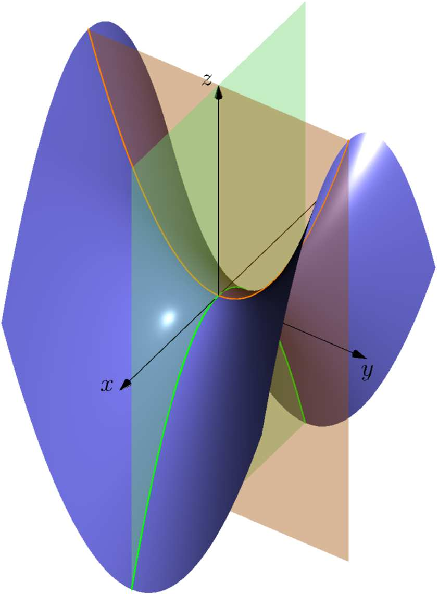
\includegraphics[width=\linewidth]{generated/asymptote/segder.pdf}
\end{image}%
\tcblower
\end{figureptx}%
%
\par
As derivadas mistas têm uma interpretação um pouco menos imediata: como vimos na \hyperref[remark-obs_apintderpar]{Nota~{\xreffont\ref{remark-obs_apintderpar}}}, a derivada parcial \(f_x(x_0,y_0)\) dá o coeficiente angular da reta tangente ao gráfico de \(g(x)=f(x,y_0)\) no ponto \(x=x_0\). A derivada de \(f_x\) em relação a \(y\) no ponto \((x_0,y_0)\) dá a taxa de variação dos coeficientes angulares da função \(g(x)\) no ponto \(x=x_0\) quando variamos \(y\), mantendo \(x_0\) fixado.%
\par
Interpretação análoga se dá para a derivada mista na outra ordem.%
\end{remark}
Com a obervação acima é de se esperar que não haja nenhuma relação entre os valores das duas derivadas mistas de uma função no mesmo ponto. Eventualmente uma delas pode existir e a outra nem isso!%
\begin{example}{Exemplo}{}{example-exemplo_derseg}%
Seja \(f(x,y)=x^3-3xy+5x^2y^4+3\). Calculemos as derivadas mistas de segunda ordem:%
\begin{align*}
f_x(x,y)&=3x^2-3y+10xy^4\implies
f_{xy}(x,y)=-3+40xy^3;\\
f_y(x,y)&=-3x+20x^2y^3\implies
f_{yx}(x,y)=-3+40xy^3,
\end{align*}
ou seja, as derivadas mistas são iguais em cada ponto!%
\end{example}
Sorte? Provavelmente sim, já que o \hyperlink{exercise-dif14}{Exercício~{\xreffont 1.5.14}}, mostra que nem sempre isso acontece. Vamos estabelecer uma nomenclatura utilizada no resultado que garante condições suficientes para que as derivadas mistas coincidam em cada ponto.%
\begin{definition}{Definição}{(Funções de classe \(\mathscr{C}^k\)).}{definition-def_classeCk}%
Sejam \(f\colon A\subseteq\R^2\to\R\) uma função e \((x_0,y_0)\) um ponto no interior de \(A\). Dizemos que \(f\) é \terminology{de classe \(\mathscr{C}^k\) em \((x_0,y_0)\)} se todas as derivadas parciais de ordem até \(k\) são contínuas em \((x_0,y_0)\).%
\end{definition}
Temos então o%
\begin{theorem}{Teorema}{(Schwarz).}{}{theorem-teo_schwarz}%
Se \(f\colon A\subseteq\R^2\to\R\) é uma função de classe \(\mathscr{C}^2\) em \((x_0,y_0)\), então \(f_{xy}(x_0,y_0)=f_{yx}(x_0,y_0)\).%
\end{theorem}
\begin{proof}{Demonstração}{}{proof-teo_schwarz-c}
Seguindo diretamente das definições, temos%
\begin{align*}
\dfrac{\partial^2 f}{\partial y\partial
x}(x_0,y_0)
&=\lim\limits_{k\to
0}\dfrac{f_x(x_0,y_0+k)-f_x(x_0,y_0)}{k}\\
&=\lim\limits_{k\to
0}\dfrac{\lim\limits_{h\to
0}\frac{f(x_0+h,y_0+k)-f(x_0,y_0+k)}{h}-\lim\limits_{h\to
0}\frac{f(x_0+h,y_0)-f(x_0,y_0)}{h}}{k}\\
&=\lim\limits_{k\to 0}\lim\limits_{h\to 0}
\dfrac{f(x_0+h,y_0+k)-f(x_0,y_0+k)-f(x_0+h,y_0)+f(x_0,y_0)}{hk}\\
&=\lim\limits_{k\to 0}\lim\limits_{h\to 0}
\dfrac{\psi(y_0+k)-\psi(y_0)}{hk}\stackrel{(\ast)}{=},
\end{align*}
onde \(\psi(y)=f(x_0+h,y)-f(x_0,y)\) é uma função derivável. Para cada \(k\) fixado, aplicando o TVM temos que%
\begin{equation*}
\psi(y_0+k)-\psi(y_0)=\psi'(\overline{y})k=\big(f_y(x_0+h,\overline{y})
-f_y(x_0,\overline{y})\big)k.
\end{equation*}
Voltando no limite acima, temos%
\begin{align*}
\dfrac{\partial^2 f}{\partial y\partial
x}(x_0,y_0)
&\stackrel{(\ast)}{=}\lim\limits_{k\to 0}\lim\limits_{h\to 0}
\dfrac{\big(f_y(x_0+h,\overline{y})
-f_y(x_0,\overline{y})\big)k}{hk}\\
&=\lim\limits_{k\to
0}\lim\limits_{h\to 0}
\dfrac{f_y(x_0+h,\overline{y})
-f_y(x_0,\overline{y})}{h}\\
&=\lim\limits_{k\to
0}\dfrac{\partial^2 f}{\partial x\partial
y}(x_0,\overline{y})=\dfrac{\partial^2 f}{\partial x\partial
y}(x_0,y_0),
\end{align*}
pois, por hipótese, \(\dfrac{\partial^2 f}{\partial x\partial y}\) é contínua em \((x_0,y_0)\).%
\end{proof}
O exemplo a seguir mostra que a recíproca do Teorema de Schwarz é falsa.%
\begin{example}{Exemplo}{}{example-exemplo_naoschwarz}%
A função \(f(x,y)=\begin{cases}
(x^2+y^2)^2\sin\Big(\dfrac{1}{x^2+y^2}\Big),&(x,y)\neq (0,0);\\
\hfill 0,& (x,y)=(0,0)\end{cases}\) é uma função de classe \(\mathscr{C}^1\) em \((0,0)\), satisfaz \(f_{xy}(0,0)=f_{yx}(0,0)\), mas não é de classe \(\mathscr{C}^2\) em \((0,0)\).%
\par
Calculando pelas regras de derivação e pela definição onde for pertinente, temos%
\begin{align*}
\dfrac{\partial f}{\partial x}(x,y)
&=\begin{cases}4x(x^2+y^2)\sin\Big(\dfrac{1}{x^2+y^2}\Big)-
2x\cos\Big(\dfrac{1}{x^2+y^2}\Big),&(x,y)\neq
(0,0);\\ \hfill 0,& (x,y)=(0,0)\end{cases};\\
\dfrac{\partial f}{\partial y}(x,y)
&=\begin{cases}4y(x^2+y^2)\sin\Big(\dfrac{1}{x^2+y^2}\Big)-
2y\cos\Big(\dfrac{1}{x^2+y^2}\Big),&(x,y)\neq
(0,0);\\ \hfill 0,& (x,y)=(0,0)\end{cases}.
\end{align*}
É relativamente imediato verificar a continuidade das funções acima e portanto que é uma função de classe \(\mathscr{C}^1\) em \((0,0)\).%
\par
Calculando uma das derivadas mistas na origem, temos%
\begin{align*}
\dfrac{\partial^2 f}{\partial y\partial x}(0,0)
&=\lim\limits_{k\to 0}\dfrac{f_x(0,0+k)-f_x(0,0)}{k}=0;\\
\dfrac{\partial^2 f}{\partial x\partial y}(0,0)
&=\lim\limits_{h\to 0}\dfrac{f_y(0+h,0)-f_y(0,0)}{h}=0;
\end{align*}
%
\par
Finalmente, escrevemos a derivada segunda \(f_yx(x,y)\) para analisar sua continuidade.%
\begin{equation*}
\dfrac{\partial^2 f}{\partial
y\partial x}(x,y)= \begin{cases}
8xy-\dfrac{4xy}{(x^2+y^2)^2}\sin\Big(\dfrac{1}{x^2+y^2}\Big),&(x,y)\neq
(0,0);\\ \hfill 0,& (x,y)=(0,0) \end{cases},
\end{equation*}
onde é relativamente fácil ver que a segunda parcela não tem limite na origem, enquanto a primeira tende a \(0\), mostrando que \(\dfrac{\partial^2 f}{\partial y\partial x}\) não tem limite em \((0,0)\), logo não pode ser contínua ali.%
\end{example}
Com um pouco de imaginação você consegue generalizar as definições e resultados aqui apresentados para funções com mais de duas variáveis e também para derivadas de ordem \(k> 2\).%
\end{sectionptx}
%
%
\typeout{************************************************}
\typeout{Seção A.6 Regras da Cadeia e Derivadas direcionais}
\typeout{************************************************}
%
\begin{sectionptx}{Seção}{Regras da Cadeia e Derivadas direcionais}{}{Regras da Cadeia e Derivadas direcionais}{}{}{section-ap_cadeiadir}
\begin{introduction}{}%
Nesta seção vamos apresentar a derivação da composta de uma função de duas variáveis com uma curva plana e, como consequência, maneiras de derivar outras compostas e também derivadas em direções que não são paralelas aos eixos coordenados, sempre ilustrados com exemplos e contra-exemplos.%
\end{introduction}%
Começamos com uma definição e uma lema técnico que permitirá enunciar o resultado principal desta seção.%
\begin{definition}{Definição}{(Vetor Gradiente).}{definition-def_gradiente}%
Seja \(f\colon A\subseteq\R^2\to\R\) uma função que admite derivadas pariciais em \((x_0,y_0)\in A\). O \terminology{gradiente} de \(f\) em \((x_0,y_0)\) é o vetor%
\begin{equation*}
\nabla f(x_0,y_0)=\Big(\dfrac{\partial f}{\partial
x}(x_0,y_0),\dfrac{\partial f}{\partial y}(x_0,y_0)\Big).
\end{equation*}
%
\end{definition}
\begin{lemma}{Lema}{}{}{lemma-lem_cadeia}%
Seja \(f\colon A\subseteq\R^2\to\R\) uma função diferenciável em \((x_0,y_0)\), então existe \(\phi\colon
A\subseteq\R^2\to\R\), contínua em \((x_0,y_0)\) tal que%
\begin{equation*}
f(x,y)=f(x_0,y_0)+\big\langle\nabla
f(x_0,y_0),(x-x_0,y-y_0)\big\rangle+\phi(x,y)\big\|(x-x_0,y-y_0)\big\|.
\end{equation*}
%
\end{lemma}
\begin{proof}{Demonstração}{}{proof-lem_cadeia-b}
Queremos construir uma função \(\phi\) que verifique a propriedade acima. Se \((x,y)\neq (x_0,y_0)\), é claro que tal função deve satisfazer%
\begin{equation*}
\phi(x,y)=\dfrac{f(x,y)-f(x_0,y_0)-\big\langle\nabla
f(x_0,y_0),(x-x_0,y-y_0)\big\rangle}{\big\|(x-x_0,y-y_0)\big\|}.
\end{equation*}
O valor de \(\phi\) em \((x_0,y_0)\) deve ser tal que a função seja contínua nesse ponto, ou seja, \(\phi(x_0,y_0)=\lim\limits_{(x,y)\to (x_0,y_0)}
\phi(x,y)\). Fazendo \(x=x_0+h\) e \(y=y_0+k\), vemos que este limite é nada mais que o limite da \hyperref[definition-def_diff]{Definição~{\xreffont\ref{definition-def_diff}}}, que é zero aqui, uma vez que \(f\) é diferenciável em \((x_0,y_0)\).%
\par
Assim, definimos%
\begin{equation*}
\phi(x,y)=\begin{cases}
\dfrac{f(x,y)-f(x_0,y_0)-\big\langle\nabla
f(x_0,y_0),(x-x_0,y-y_0)\big\rangle}{\big\|(x-x_0,y-y_0)\big\|},&(x,y)\neq
(x_0,y_0)\\
\hfill 0,& (x,y)=(x_0,y_0).
\end{cases}\qedhere
\end{equation*}
%
\end{proof}
\begin{remark}{Nota}{}{remark-ap_cadeiadir-f}%
Note inicialmente que as duas primeiras parcelas do lado direito na expressão em destaque são exatamente as parcelas independentes de \(z\) na equação do plano tangente gráfico de \(f\) em \((x_0,y_0)\).%
\par
Com isto, este enunciado é uma generalização natural do que acontece com funções de uma variável, quando olhamos para o polinômio de Taylor de ordem 1: o erro na aproximação, ali pela reta tangente, aqui pelo plano tangente, dá um erro que tende a zero "mais rapidamente" do que \((x,y)\) se aproxima de \((x_0,y_0)\).%
\end{remark}
\begin{theorem}{Teorema}{(Regra da Cadeia).}{}{theorem-teo_cadeia}%
Sejam \(f\colon A\subseteq\R^2\to\R\) uma função diferenciável em \((x_0,y_0)\) e \(\gamma\colon
I\subseteq\R\to\R\) derivável em \(t_0\in I\) tal que \(\gamma(t_0)=(x_0,y_0)\). Então \(f\circ\gamma \) é derivável em \(t_0\) e%
\begin{equation*}
(f\circ\gamma)'(t_0)=\big\langle\nabla
f(x_0,y_0),\gamma'(t_0)\big\rangle.
\end{equation*}
%
\end{theorem}
\begin{proof}{Demonstração}{}{proof-teo_cadeia-c}
Começamos recordando que%
\begin{equation*}
(f\circ\gamma)'(t_0)=\lim\limits_{t\to t_0}
\dfrac{(f\circ\gamma)(t)-(f\circ\gamma)(t_0)}{t-t_0}.
\end{equation*}
%
\par
Podemos aplicar o \hyperref[lemma-lem_cadeia]{Lema~{\xreffont\ref{lemma-lem_cadeia}}} aos termos do numerador acima, com \((x,y)=\gamma(t)\) e \((x_0,y_0)=\gamma(t_0)\), obtendo%
\begin{align*}
(f\circ\gamma)'(t_0)&
=\lim\limits_{t\to t_0}\big\langle\nabla
f(x_0,y_0),\dfrac{\gamma(t)-\gamma(t_0)}{t-t_0}\big\rangle+\phi\big(\gamma(t)\big)\dfrac{\big\|\gamma(t)-\gamma(t_0)\big\|}{t-t_0}\\
&
=\big\langle\nabla f(x_0,y_0),\gamma'(t_0)\big\rangle+
\lim\limits_{t\to t_0}
\phi\big(\gamma(t)\big)
\Big\|\dfrac{\gamma(t)-\gamma(t_0)}
{t-t_0}\Big\|\dfrac{|t-t_0|}{t-t_0}\\
&
=\big\langle\nabla f(x_0,y_0),\gamma'(t0)\big\rangle,
\end{align*}
pois \(\lim\limits_{t\to
t_0}\phi\big(\gamma(t)\big)=\phi(x_0,y_0)=0\), \(\lim\limits_{t\to t_0}\Big\|\dfrac{\gamma(t)-\gamma(t_0)}
{t-t_0}\Big\|=\big\|\gamma'(t_0)\|\) e \(\dfrac{|t-t_0|}{t-t_0}\) é limitado.%
\end{proof}
\begin{remark}{Nota}{}{remark-ap_cadeiadir-h}%
Uma interpretação para a Regra da Cadeia apresentada acima é que a derivada, ou taxa de variação, de \(f\) ao longo de uma curva está ligada com a projeção ortogonal do gradiente de \(f\) sobre o vetor velocidade da curva.%
\begin{figureptx}{Figura}{A composta \(f\circ\gamma\).}{figure-fig_cadeiadir}{}%
\begin{image}{0.05}{0.9}{0.05}{}%
\resizebox{\linewidth}{!}{%
\begin{tikzpicture}
       \draw (-3,2) -- (-2,0) node[left] {$t$};
       \filldraw (-2.5,1) circle (1pt) node[left]{$t_0$};
       \draw[->] (-.5,0) -- (2.5,0) node[below] {$x$};
       \draw[->] (0,-.5) -- (0,2) node[right] {$y$};
       \draw[red, thick,variable=\t,domain=0.7:2,samples=10,smooth]
       plot (\t,{1/2*(-3*sin(\t r)+sin(5*\t r))+2});
       \draw[->] (-2.25,1) to[bend left] node[above]{$\gamma$}
(-.75,1.25);
       \filldraw (1.5,{1/2*(-3*sin(1.5 r)+sin(5*1.5 r))+2}) circle (1pt)
       node[above left]{$\gamma(t_0)$};
\draw[thick,->,blue] (1.5,{1/2*(-3*sin(1.5 r)+sin(5*1.5
r))+2}) -- ++(0.5,{0.5*(-3/2*cos (1.5 r)+5/2*cos(5*1.5 r))})
node [right] {$\gamma'(t_0)$};
\draw[thick,->,blue] (1.5,{1/2*(-3*sin(1.5 r)+sin(5*1.5
r))+2}) -- ++(0.5,1.5)
node [right] {$\nabla f(x_0,y_0)$};
       \draw (4,0) -- (5,2) node[right] {$z$};
       \filldraw (4.5,1) circle (1pt)
       node[right]{$f\big(\gamma(t_0)\big)$};
       \draw[->] (2.75,.75) to[bend left] node[below]{$f$} (4,1.25);
\end{tikzpicture}
}%
\end{image}%
\tcblower
\end{figureptx}%
\end{remark}
Além de seu valor no cálculo de derivadas de compostas, a Regra da Cadeia é uma poderosa ferramenta para mostrar que uma função não é diferenciável. Veja como no exemplo abaixo:%
\begin{example}{Exemplo}{}{example-exemplo_cadeianaodiff}%
A função \(f(x,y)=\begin{cases}
\dfrac{x^3}{x^2+y^2},&(x,y)\neq (0,0);\\ \hfill 0,&
(x,y)=(0,0)\end{cases}\) não é diferenciável na origem. De fato, \(\gamma(t)=(t,t)\), é uma curva derivável tal que \(\gamma(0)=(0,0)\) e \(\gamma'(0)=(1,1)\). Temos, calculando explicitamente, que%
\begin{equation*}
(f\circ \gamma)(t)=\dfrac{t}{2}\implies
(f\circ \gamma)'(0)=\dfrac{1}{2}\text{.}
\end{equation*}
No \hyperlink{exercise-dif5}{Exercício~{\xreffont 1.5.5}} calculamos as derivadas parciais de \(f\), obtendo \(\nabla
f(0,0)=(1,0)\). derivadas parciais em \((0,0)\), mas não é contínua em \((0,0)\). Assim,%
\begin{equation*}
\big\langle\nabla
f(0,0),\gamma'(0)\big\rangle=1\neq\frac{1}{2}=(f\circ
\gamma)'(0).
\end{equation*}
Se \(f\) fosse derivável na origem, a igualdade deveria valer para qualquer curva nas condições do enunciado do \hyperref[theorem-teo_cadeia]{Teorema~{\xreffont\ref{theorem-teo_cadeia}}}%
\end{example}
No caso especial em que a curva considerada é uma curva de nível da função temos um resultado bastante interessante:%
\begin{corollary}{Corolário}{(\(\nabla f\perp f^{-1}(c)\)).}{}{corollary-cor_cadeiagradniv}%
Sejam \(f\colon A\subseteq\R^2\to\R\) uma função diferenciável e \(\gamma\colon I\subseteq\R\to\R^2\), que é uma curva derivável tal que \(\mathrm{Im}\gamma\subset f^{-1}(c)\) (a curva parametriza parte de uma curva de nível de \(f\)). Então,%
\begin{equation*}
\Big\langle\nabla
f\big(\gamma(t)\big),\gamma'(t)\Big\rangle=0,
\end{equation*}
para todo \(t\in I\).\begin{remark}{Nota}{}{remark-cor_cadeiagradniv-d}%
Este é o famoso resultado que se traduz na frase "\emph{O gradiente é perpendicular às curvas de nível.}".\end{remark}
\end{corollary}
\begin{proof}{Demonstração}{}{proof-cor_cadeiagradniv-c}
Basta observar que, nas condições do enunciado, temos \((f\circ\gamma)(t)=c\in\R\) e portanto \((f\circ\gamma)'(t)=0\) para todo \(t\in I\). O resultado segue disto aplicado ao \hyperref[theorem-teo_cadeia]{Teorema~{\xreffont\ref{theorem-teo_cadeia}}}.\end{proof}
\begin{example}{Exemplo}{}{example-exemplo_cadeianivel}%
Seja \(f(x,y)=x^2+y^2\), que é diferenciável em todo seu domínio. Sua curva de nível \(c<0\) é um círculo centrado na origem e de raio \(\sqrt{c}\), que pode ser parametrizado por \(\gamma(t)=\sqrt{c}(\cos t, \sin t)\), \(t\in
[0,2\pi]\). Como \(\nabla f(x,y)=(2x,2y)\) e \(\gamma'(t)=\sqrt{c}(-\sin t, \cos t)\), temos%
\begin{equation*}
\Big\langle\nabla
f\big(\gamma(t)\big),\gamma'(t)\Big\rangle=\big\langle
(2\sqrt{c}\cos t, 2\sqrt{c}\sin t),(-\sqrt{c}\sin t,\sqrt{c}\cos
t)\big\rangle =0
\end{equation*}
%
\begin{figureptx}{Figura}{O gradiente ao longo de uma curva de nível.}{figure-fig_cadeianivel}{}%
\begin{image}{0.25}{0.5}{0.25}{}%
\resizebox{\linewidth}{!}{%
\begin{tikzpicture}
       \draw[->] (-1.5,0) -- (1.5,0) node[below] {$x$};
       \draw[->] (0,-1.5) -- (0,1.5) node[right] {$y$};
\draw[red] (0,0) circle (1) node[xshift=30,yshift=-30] {$f^{-1}(c)$};
\filldraw ({cos(30)},{sin(30)}) circle (1pt);
\draw[->,blue] ({cos(30)},{sin(30)}) -- ++ ({-sin(30)},{cos(30)})
node[right] {$\gamma'(t)$};
\draw[->,blue] ({cos(30)},{sin(30)}) -- ++ ({2*cos(30)},{2*sin(30)})
node[above] {$\nabla f\big(\gamma(t)\big)$};
\end{tikzpicture}
}%
\end{image}%
\tcblower
\end{figureptx}%
Note que nessas condições a projeção do gradiente na direção tangente à da curva é nula, ou seja, que caminha ao longo de uma curva de nível "não sente" as derivadas de \(f\) (e por isso ela é constante ao longo dessa trajetória.%
\end{example}
\begin{corollary}{Corolário}{}{}{corollary-cor_cadeiaturbo}%
Sejam \(g,h\colon B\subseteq\R^2\to\R\) funções diferenciáveis em \((u_0,v_0)\) e \(f\colon A\subseteq\R^2\to\R\) diferenciável em \(\big(g(u_0,v_0),h(u_0,v_0)\big)\). Então a função%
\begin{equation*}
F\colon B\to\R,\quad
F(u,v)=f\big(g(u,v),h(u,v)\big)
\end{equation*}
é diferenciável em \((u_0,v_0)\) e%
\begin{align*}
\dfrac{\partial F}{\partial u}(u_0,v_0)
=\dfrac{\partial f}{\partial
x}\big(g(u_0,v_0),&h(u_0,v_0)\big)\dfrac{\partial g}{\partial
u}(u_0,v_0)+\\
&\dfrac{\partial f}{\partial
y}\big(g(u_0,v_0),h(u_0,v_0)\big)\dfrac{\partial h}{\partial
u}(u_0,v_0);\\
\dfrac{\partial F}{\partial v}(u_0,v_0)
=\dfrac{\partial f}{\partial
x}\big(g(u_0,v_0),&h(u_0,v_0)\big)\dfrac{\partial g}{\partial
v}(u_0,v_0)+\\
&
\dfrac{\partial f}{\partial
y}\big(g(u_0,v_0),h(u_0,v_0)\big)\dfrac{\partial h}{\partial
v}(u_0,v_0).
\end{align*}
\begin{remark}{Nota}{}{remark-cor_cadeiaturbo-c}%
Omitindo os pontos de aplicação (tenha cuidado ao fazer isso!) e, escrevendo \(x(u,v)=g(u,v)\), \(y(u,v)=h(u,v)\) e (abusando muito!) \(f(u,v)=f\big(g(u,v),h(u,v)\big)\), temos uma notação mais sintética para as expressões acima:%
\begin{equation*}
\dfrac{\partial f}{\partial u}=\dfrac{\partial f}{\partial x}
\dfrac{\partial x}{\partial u}+\dfrac{\partial f}{\partial y}
\dfrac{\partial y}{\partial u};\qquad
\dfrac{\partial f}{\partial v}=\dfrac{\partial f}{\partial x}
\dfrac{\partial x}{\partial v}+\dfrac{\partial f}{\partial y}
\dfrac{\partial y}{\partial v}.
\end{equation*}
%
\par
De maneira ainda mais curta, podemos escrever%
\begin{equation}
f_u=f_x x_u+f_y y_u;\quad f_v=f_x x_v+f_y
y_v.\label{men-eq_gradparc}
\end{equation}
%
\end{remark}
\end{corollary}
\begin{proof}{Demonstração}{}{proof-cor_cadeiaturbo-b}
Lembrando que as derivadas parciais deixam uma das variáveis fixadas, podemos aplicar o \hyperref[theorem-teo_cadeia]{Teorema~{\xreffont\ref{theorem-teo_cadeia}}} a cada uma das curvas indicadas no plano \(Oxy\) da figura abaixo. \begin{figureptx}{Figura}{A composta \(f\circ\gamma\).}{figure-fig_cadeiaturbo}{}%
\begin{image}{0.05}{0.9}{0.05}{}%
\resizebox{\linewidth}{!}{%
    \begin{tikzpicture}
           \draw[->] (-5,0) -- (-2,0) node[below] {$u$};
           \draw[->] (-4.5,-.5) -- (-4.5,2) node[right] {$v$};
    \filldraw (-3.5,1) circle (1pt);
    \draw[dashed] (-3.5,1) -- (-3.5,0) node[below]{$u_0$};
    \draw[dashed] (-3.5,1) -- (-4.5,1) node[left]{$v_0$};
    \draw[red] (-4,1)--(-3,1);
    \draw[blue] (-3.5,0.5)--(-3.5,1.5);
    
    \draw[->] (-3.45,1.05) to[bend left] (1.45,0.05);
    \draw[->] (-3.45,1.05) to[bend left] (-0.05,1.25);

    \draw[->] (-.5,0) -- (2.5,0) node[below] {$x$};
           \draw[->] (0,-.5) -- (0,2) node[right] {$y$};
    \filldraw (1.5,0) circle (1pt) node[above right]{$g(u_0,v_0)$};
    \filldraw (0,1.25) circle (1pt) node[above right]{$h(u_0,v_0)$};
           \filldraw (1.5,1.25) circle (1pt);
    \draw[dashed] (1.5,1.25) -- (1.5,0);
    \draw[dashed] (1.5,1.25) -- (0,1.25);
    
    \draw[red,domain=1.25:1.75,samples=10,smooth] plot
    (\x,{exp(\x)*1.25/exp(1.5)});
    \draw[blue,domain=1.25:1.75,samples=10,smooth] plot
    (\x,{1.5*1.25/\x});
           \draw[->] (-2.5,-2) -- (.5,-2) node[above] {$z$};
           \draw[->] (1.45,-0.1) -- node[right]{$f$} (-0.95,-1.95);
    \filldraw (-1,-2) circle (1pt) node[below, xshift=40]{$f\big(g(u_0,v_0),h(u_0,v_0)\big)$};
    \end{tikzpicture}
}%
\end{image}%
\tcblower
\end{figureptx}%
%
\par
Considerando então a curva \(\beta(u)=\big(g(u,v_0),h(u,v_0)\big)\), para a qual \(\beta'(u)=\big(g_u(u,v_0),h_u(u,v_0)\big)\) e aplicando a Regra da Cadeia do \hyperref[theorem-teo_cadeia]{Teorema~{\xreffont\ref{theorem-teo_cadeia}}}, temos%
\begin{align*}
\dfrac{\partial F}{\partial u}(u_0,v_0)&
=(f\circ\beta)'(u_0)\\
&=\big\langle \nabla f(x_0,y_0),\beta'(u_0)\big\rangle=
\dfrac{\partial f}{\partial x}(x_0,y_0)\dfrac{\partial g}{\partial
u}(u_0,v_0)+\dfrac{\partial f}{\partial y}(x_0,y_0)\dfrac{\partial
h}{\partial u}(u_0,v_0),
\end{align*}
onde \((x_0,y_0)=\big(g(u_0,v_0),h(u_0,v_0)\big)\).%
\par
Procedendo de maneira análoga para a curva \(\gamma(v)=\big(g(u_0,v),h(u_0,v)\big)\), obtemos a expressão para a derivada em \(v\) de \(F\), no ponto \((u_0,v_0)\).%
\end{proof}
Podemos, naturalmente, calcular as \emph{derivadas segundas} de tais compostas. Para tanto, basta lembrar que vamos precisar dos gradientes de \(f_x\) e \(f_y\):%
\begin{equation*}
\nabla
f_x(x,y)=\big(f_{xx}(x,y),f_{xy}(x,y)\big); \qquad \nabla
f_x(x,y)=\big(f_{xx}(x,y),f_{xy}(x,y)\big).
\end{equation*}
Assim, com as hipóteses de derivadas parciais de \(f\) sendo diferenciáveis e \(\gamma\) admitindo segunda derivada nos respectivos pontos, e escrevendo \(\gamma(t)=\big(x(y),y(t)\big)\), temos, com a Regra da Cadeia, que%
\begin{align*}
(f\circ\gamma)''(t_0)&=\Big(\big\langle\nabla
f\big(\gamma(t)\big),\gamma'(t)\big\rangle\Big)'(t_0)\\
=&\Big(f_x\big(\gamma(t)\big)x'(t)+
f_y\big(\gamma(t)\big)y'(t)\Big)'(t_0).
\end{align*}
%
\par
Derivando cada parcela com a regra do produto e usando novamente a Regra da Cadeia (aplicada às derivadas parciais de \(f\)), temos%
\begin{align*}
\Big(f_x\big(\gamma(t)\big)&x'(t)+
f_y\big(\gamma(t)\big)y'(t)\Big)'(t_0)\\
&=\big\langle \nabla
f_x\big(\gamma(t_0)\big),\gamma'(t_0)\Big\rangle x'(t_0)+
f_x\big(\gamma(t_0)\big)x''(t_0)+\\
&\big\langle \nabla
f_y\big(\gamma(t_0)\big),\gamma'(t_0)\Big\rangle y'(t_0)+
f_y\big(\gamma(t_0)\big)y''(t_0).
\end{align*}
%
\par
Abrindo os produtos internos usando \hyperref[men-eq_gradparc]{({\xreffont\ref{men-eq_gradparc}})} e escrevendo tudo nas notações mais sintéticas (cuidado com os pontos de aplicação!), temos%
\begin{align}
(f\circ\gamma)''(t_0)
=f_{xx}&(x_0,y_0)\big(x'(t_0)\big)^2+f_{yy}(x_0,y_0)\big(y'(t_0)\big)^2+\notag\\
&\big(f_{xy}(x_0,y_0)+f_{yx}(x_0,y_0)\big)x'(t_0)y'(t_0)+\notag\\
&f_x\big(\gamma(t_0)\big)x''(t_0)+
f_y\big(\gamma(t_0)\big)y''(t_0).\label{mrow-eq_cadeiaderseg}
\end{align}
%
\par
No caso especial em que \(f\) é de classe \(\mathscr{C}^2\) em \((x_0,y_0)\), usamos o \hyperref[theorem-teo_schwarz]{Teorema~{\xreffont\ref{theorem-teo_schwarz}}} para escrever%
\begin{align}
(f\circ\gamma)''(&t_0)=\notag\\
&f_{xx}(x_0,y_0)\big(x'(t_0)\big)^2+f_{yy}(x_0,y_0)\big(y'(t_0)\big)^2+\notag\\
&2f_{xy}(x_0,y_0)x'(t_0)y'(t_0)+f_x\big(\gamma(t_0)\big)x''(t_0)+
f_y\big(\gamma(t_0)\big)y''(t_0).\label{mrow-eq_cadeiadersegc2}
\end{align}
%
\par
Assim como usamos o \hyperref[theorem-teo_cadeia]{Teorema~{\xreffont\ref{theorem-teo_cadeia}}} para provar o \hyperref[corollary-cor_cadeiaturbo]{Corolário~{\xreffont\ref{corollary-cor_cadeiaturbo}}}, é possível usar as expressões acima para calcular as derivadas parciais de segunda ordem de compostas do tipo \(f\big(g(u,v),h(u,v)\big)\). Fazemos isso no \hyperlink{exercise-cadeia6}{Exercício~{\xreffont 1.6.6}}.%
\begin{definition}{Definição}{(Derivada Direcional).}{definition-def_derdir}%
Sejam \(f\colon A\subseteq\R^2\to\R\) uma função e \(\vec{v}\in\R^2\) um vetor unitário. A \terminology{derivada direcional} de \(f\), na direção de \(\vec{v}\), em \((x_0,y_0)\) é dada por%
\begin{equation*}
\dfrac{\partial f}{\partial
\vec{v}}(x_0,y_0)=\lim\limits_{t\to
0}\dfrac{f\big((x_0,y_0)+t\vec{v}\big)-f(x_0,y_0)}{t}.
\end{equation*}
%
\begin{remark}{Nota}{}{remark-def_derdir-c}%
No caso especial em que \(\vec{v}=\vec{e_1}=(1,0)\) ou \(\vec{v}=\vec{e_2}=(0,1)\), recuperamos, respectivamente, \(f_x(x_0,y_0)\) e \(f_y(x_0,y_0)\). A interpretação geométrica é análoga à feita na \hyperref[remark-obs_apintderpar]{Nota~{\xreffont\ref{remark-obs_apintderpar}}}, com cortes por planos não paralelos aos eixos \(Ox\) ou \(Oy\).\end{remark}
\end{definition}
Quando a função \(f\) é diferenciável, o vetor gradiente determina completamente as derivadas direcionais:%
\begin{proposition}{Proposição}{}{}{proposition-prop_derdir}%
Sejam \(f\colon A\subseteq\R^2\to\R\) uma função diferenciável em \((x_0,y_0)\) e \(\vec{v}\) um vetor unitário. Então%
\begin{equation*}
\dfrac{\partial f}{\partial\vec{v}}(x_0,y_0)=\big\langle\nabla
f(x_0,y_0),\vec{v}\big\rangle.
\end{equation*}
\end{proposition}
\begin{proof}{Demonstração}{}{proof-prop_derdir-b}
Basta parametrizar um segmento de reta que passa por \((x_0,y_0)\) e tem a direção de \(\vec{v}\): \(\gamma(t)=(x_0,y_0)+t\vec{v}\), \(t\in
(-\epsilon,\epsilon)\) (com \(\epsilon > 0\)). Assim,%
\begin{equation*}
\dfrac{\partial f}{\partial
\vec{v}}(x_0,y_0)=\lim\limits_{t\to
0}\dfrac{f\big((x_0,y_0)+t\vec{v}\big)-f(x_0,y_0)}{t}=(f\circ\gamma)'(t_0)=\big\langle\nabla
f(x_0,y_0),\vec{v}\big\rangle.\qedhere
\end{equation*}
\end{proof}
\begin{remark}{Nota}{}{remark-ap_cadeiadir-w}%
Se \(\gamma:I\subseteq\R\to\R^2\) é qualquer curva derivável em \(t_0\in I\) tal que \(\gamma(t_0)=(x_0,y_0)\) e \(\gamma'(t_0)=\vec{v}\), então%
\begin{equation*}
(f\circ\gamma)'(t_0)=\big\langle\nabla
f(x_0,y_0),\gamma'(t_0)\big\rangle=\big\langle\nabla
f(x_0,y_0),\vec{v}\big\rangle=\dfrac{\partial f}{\partial
\vec{v}}(x_0,y_0),
\end{equation*}
ou seja, a derivada de \(f\) ao longo de \(\gamma\) em \(t_0\) depende apenas de \(\gamma'(t_0)\). Em outras palavras, se duas curvas passam por um mesmo ponto do plano e têm o mesmo tangente nesse ponto, então qualquer função diferenciável terá a mesma derivada quando composta com essas curvas naquele ponto.\end{remark}
\begin{remark}{Nota}{}{remark-ap_cadeiadir-x}%
A existência de derivadas direcionais em todas as direções não garante diferenciabilidade. Por exemplo, vimos que a função do \hyperlink{exercise-dif5}{Exercício~{\xreffont 1.5.5}} não é diferenciável na origem, mas admite derivadas direcionais nesse ponto em todas as direções: se \(\vec{v}=(a,b)\), com \(a^2+b^2=1\), temos:%
\begin{equation*}
\dfrac{\partial f}{\partial\vec{v}}(0,0)=\lim\limits_{t\to
0}\dfrac{f(at,bt)-f(0,0)}{t}=\lim\limits_{t\to
0}\dfrac{a^3t}{t}=a^3.
\end{equation*}
%
\par
Em vista da fórmula na \hyperref[proposition-prop_derdir]{Proposição~{\xreffont\ref{proposition-prop_derdir}}} acima, sabemos a derivada direcional de qualquer função diferenciável deve depender linearmente das coordenadas da direção em que estamos derivando.%
\end{remark}
\begin{proposition}{Proposição}{Direções de crescimento máximo.}{}{proposition-prop_crescmax}%
Se \(f\colon A\subseteq\R^2\to\R\) uma função diferenciável em \((x_0,y_0)\), então a direção em que \(f\) tem a maior taxa de variação nesse ponto é a de \(\nabla f (x_0,y_0)\).\end{proposition}
\begin{proof}{Demonstração}{}{proof-prop_crescmax-c}
Basta olhar para a definição geométrica do produto escalar em \(\R^2\):%
\begin{equation*}
\dfrac{\partial f}{\partial\vec{v}}(x_0,y_0)=\big\langle\nabla
f(x_0,y_0),\vec{v}\big\rangle=\|\nabla
f(x_0,y_0)\|\|\vec{v}\|\cos\theta\text{.}
\end{equation*}
%
\par
Como \((x_0,y_0)\) está fixado, \(\|\nabla
f(x_0,y_0)\|\|\vec{v}\|\) é uma constant e \(\|\vec{v}\|=1\). Desta forma o valor da derivada direcional depende somente \(\theta\) e assumirá seu máximo, quando \(\theta=0\), ou seja, quando \(\vec{v}=\dfrac{\nabla
f(x_0,y_0)}{\|\nabla f(x_0,y_0)\|}\)%
\end{proof}
O vídeo abaixo ilustra uma aplicação interessante da \hyperref[proposition-prop_crescmax]{Proposição~{\xreffont\ref{proposition-prop_crescmax}}}%
\begin{figureptx}{Figura}{Trajetórias ortogonais a curvas de nível.}{figure-vid_crescmax}{}%
\begin{sidebyside}{2}{0.075}{0.075}{0.17}%
\begin{sbspanel}{0.47}%
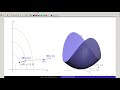
\includegraphics[width=\linewidth]{generated/youtube/video-3.jpg}
\end{sbspanel}%
\begin{sbspanel}{0.21}%

\includegraphics[width=\linewidth]{generated/qrcode/video-3.png}
\end{sbspanel}%
\end{sidebyside}%
\tcblower
\end{figureptx}%
Fechamos esta revisão com uma curiosidade:%
\begin{fact}{Fato}{Outras direções.}{}{fact-fato_outrasdir}%
Podemos generalizar um pouco o resultado acima: se uma função é diferenciável em \((x_0,y_0)\), basta conhecer as derivadas direcionais nesse ponto, em duas direções linearmente independentes, para determinarmos a derivada direcional em \((x_0,y_0)\) em qualquer direção. Para tanto, se \(\vec{u}\) e \(\vec{v}\) são vetores unitários que definem tais direções, temos que \(\big\{\vec{u},\vec{v}\big\}\) é uma base de \(\R^2\) e, portanto%
\begin{equation*}
\vec{e_1}=\alpha_1\vec{u}+\beta_1\vec{v}\quad\text{e}\quad
\vec{e_2}=\alpha_2\vec{u}+\beta_2\vec{v}.
\end{equation*}
%
\par
Desta forma, temos%
\begin{equation*}
f_x(x_0,y_0)=\dfrac{\partial
f}{\partial\vec{e_1}}(x_0,y_0)=\big\langle\nabla
f(x_0,y_0),\vec{e_1}\big\rangle=\big\langle\nabla
f(x_0,y_0),\alpha_1\vec{u}+\beta_1\vec{v}\big\rangle.
\end{equation*}
%
\par
Expandindo o produto interno pela sua linearidade e procedento de maneira análoga com o vetor \(\vec{e_2}\), temos então que%
\begin{align*}
f_x(x_0,y_0)&=\alpha_1\dfrac{\partial f}{\partial
\vec{u}}(x_0,y_0)+\beta_1\dfrac{\partial f}{\partial
\vec{v}}(x_0,y_0);\\
f_y(x_0,y_0)&=\alpha_2\dfrac{\partial f}{\partial
\vec{u}}(x_0,y_0)+\beta_2\dfrac{\partial f}{\partial
\vec{v}}(x_0,y_0).
\end{align*}
%
\par
Mais frequentemente, temos as coordenadas de \(\vec{u}\) e \(\vec{v}\) na base canônica, digamos \(\vec{u}=(a,b)\) e \(\vec{v}=(c,d)\). Procedendo de maneira inversa, temos um sistema para determinar o gradiente de \(f\) (e consequentemente todas as derivadas direcionais):%
\begin{equation*}
\begin{cases}
\dfrac{\partial f}{\partial
\vec{u}}(x_0,y_0)&=af_x(x_0,y_0)+bf_y(x_0,y_0)\\
\dfrac{\partial f}{\partial
\vec{v}}(x_0,y_0)&=cf_x(x_0,y_0)+df_y(x_0,y_0)
\end{cases},
\end{equation*}
cujas soluções são dadas invertendo-se a matriz \(\begin{pmatrix}
a&b\\ c&d \end{pmatrix}\) de coeficientes, o que é possível se e somente se os vetores \(\vec{u}\) e \(\vec{v}\) são linearmente independentes.%
\end{fact}
\end{sectionptx}
%
%
\typeout{************************************************}
\typeout{Seção A.7 Superfícies de nível e Curvas no espaço}
\typeout{************************************************}
%
\begin{sectionptx}{Seção}{Superfícies de nível e Curvas no espaço}{}{Superfícies de nível e Curvas no espaço}{}{}{section-ap_supnivel}
\begin{introduction}{}%
Extendemos aqui o conceito de curvas de nível de uma função \(f\colon A\subseteq\R^2\to\R\), visto na \hyperref[section-ap_func]{Seção~{\xreffont\ref{section-ap_func}}}, para funções de três variáveis reais, \(f\colon
A\subseteq\R^3\to\R\).%
\par
Lembramos que todos os resultados apresentados sobre continuidade, derivadas parciais, diferenciabilidade e derivadas direcionais para funções de duas variáveis generalizam-se naturalmente para funções de \(n\) variáveis (nosso caso de interesse é \(n=3\)).%
\end{introduction}%
\begin{definition}{Definição}{Superfície de nível.}{definition-sup_nivel}%
 Sejam \(f\colon A\subseteq\R^3\to\R\) e \(c\in\R\). A \terminology{superfície de nível} ou \terminology{conjunto de nível} do nível \(c\) de \(f\) é o conjunto%
\begin{equation*}
f^{-1}(c)=\{(x,y,z)\in A\colon f(x,y,z)=c\},
\end{equation*}
\end{definition}
Note que, nas condições acima, o gráfico de \(f\) está em \(\R^4\). Deste modo, as superfícies de nível vão nos ajudar a entender melhor o comportamento de tais funções. Vejamos alguns exemplo em analogia ao caso de funções a duas variáveis.%
\begin{example}{Exemplo}{}{example-ap_supnivel-e}%
Determine as curvas nível da função \(f\colon\R^3\to\R\) dada por \(f(x,y)=x^2+y^2+z^2\).%
\par\smallskip%
\noindent\textbf{\blocktitlefont Solução}.\hypertarget{solution-ap_supnivel-e-b}{}\quad{}Começamos observando que o domínio de \(f\) é todo o \(\R^3\) e sua imagem é o conjunto dos reais não-negativos, indicado por \(\R_{\geq 0}\). Com isso, temos \(f^{-1}(c)=\emptyset\), se \(c< 0\). Vejamos o que acontece com \(c\geq0\):%
\begin{itemize}[label=\textbullet]
\item{}\(c=0\): \(f(x,y,z)=0\iff x^2+y^2+z^2=0\iff
(x,y,z)=(0,0,0)\);%
\item{}\(c>0\): \(f(x,y,z)=c\iff x^2+y^2+z^2=c\). Neste caso, as soluções são exatamente pontos da esfera de raio \(\sqrt{c}\), centrada na origem.%
\end{itemize}
Observamos então que cada ponto de \(\R^3\) pertence a um e somente um conjunto de nível de \(f(x,y,z)=x^2+y^2+z^2\). \begin{figureptx}{Figura}{Conjuntos de nível de \(f\).}{figure-fig_apesffol}{}%
\begin{image}{0.25}{0.5}{0.25}{}%
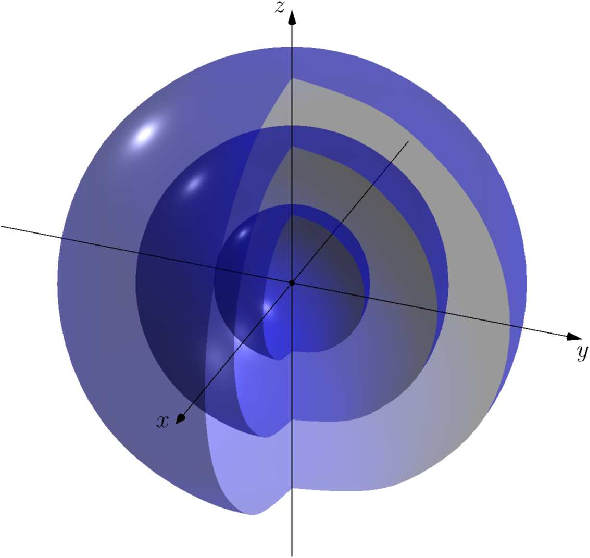
\includegraphics[width=\linewidth]{generated/asymptote/apesffol.pdf}
\end{image}%
\tcblower
\end{figureptx}%
%
\end{example}
\begin{example}{Exemplo}{}{example-ap_supnivel-f}%
Determine as curvas nível da função \(f\colon\R^3\to\R\) dada por \(f(x,y)=x^2+y^2-z^2\).%
\par\smallskip%
\noindent\textbf{\blocktitlefont Solução}.\hypertarget{solution-ap_supnivel-f-b}{}\quad{}Começamos observando que o domínio de \(f\) é todo o \(\R^3\) e sua imagem é o conjunto de todos os reais, indicado por \(\R_{\geq 0}\). Com isso, temos%
\begin{itemize}[label=\textbullet]
\item{}\(c> 0\): \(f(x,y,z)=c \iff
x^2+y^2-z^2=c\). Neste caso, o conjunto solução é um \emph{hiperboloide de uma folha}.%
\item{}\(c=0\): \(f(x,y,z)=0\iff x^2+y^2-z^2=0\), a equação do cone reto;%
\item{}\(c<0\): \(f(x,y,z)=c\iff x^2+y^2-z^2=c\), que define um hiperboloide de duas folhas.%
\end{itemize}
Novamente observamos então que cada ponto de \(\R^3\) pertence a um e somente um conjunto de nível de \(f(x,y,z)=x^2+y^2-z^2\). \begin{figureptx}{Figura}{Conjuntos de nível de \(f\).}{figure-fig_aphipfol}{}%
\begin{image}{0.25}{0.5}{0.25}{}%
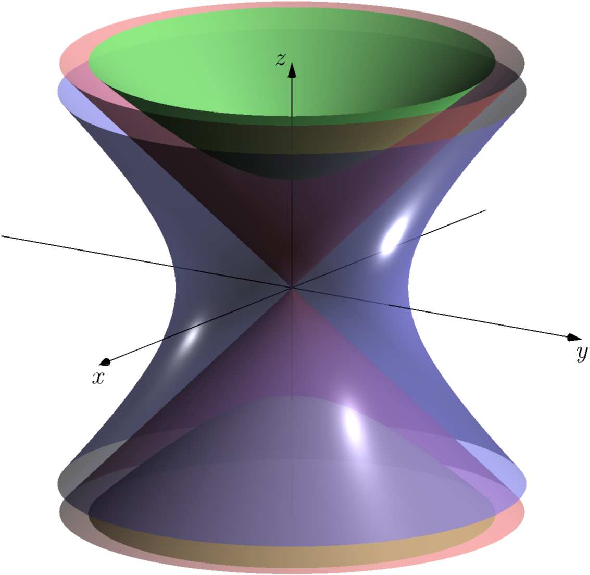
\includegraphics[width=\linewidth]{generated/asymptote/aphipfol.pdf}
\end{image}%
\tcblower
\end{figureptx}%
%
\end{example}
Os dois exemplos acima são casos especiais das \emph{superfícies quádricas}. Um tabela com suas equações reduzidas para os casos não degenerados pode ser vista \href{https://www.ime.usp.br/\~lymber/teaching/quadricas/index.html}{aqui}\footnote{\nolinkurl{ime.usp.br/\~lymber/teaching/quadriicas.html}\label{fn-ap_supnivel-g-c}}. Em Álgebra Linear II você verá um método que explicita um sistema de coordenadas onde a equação de uma dada superfície quádrica se escreve na forma reduzida.%
\par
Se \(f\colon A\subseteq\R^3\to\R\) é uma função diferenciável e \(\gamma\colon I\subseteq\R\to\R^3\) é uma curva derivável tal que a imagem de \(\gamma\) está contida na superfície de nível \(c\) de \(f\), então \(f\big(\gamma(t)\big)=c\), para todo \(t\in
I\). Utilizando uma generalização (relativamente óbvia) do \hyperref[theorem-teo_cadeia]{Teorema~{\xreffont\ref{theorem-teo_cadeia}}} para o \(\R^3\) , temos que%
\begin{equation*}
0=(f\circ\gamma)'(t)=\Big\langle\nabla
f\big(\gamma(t)\big),\gamma'(t)\Big\rangle.
\end{equation*}
Isto mostra que o vetor \(\nabla f\) é ortogonal a todas as curvas cuja imagem está contida numa superfície de nível de \(f\), motivando naturalmente a%
\begin{definition}{Definição}{Plano Tangente a uma superficie de nível.}{definition-def_planotangente}%
 Sejam \(f\colon A\subseteq\R^3\to\R\) uma função diferenciável e \((x_0,y_0,z_0)\in f^{-1}(c)\). O \terminology{plano tangente à superfície de nível \(c\) de \(f\) no ponto \((x_0,y_0,z_0)\)} é o conjunto dos vetores tangentes a todas as curvas cuja imagens contenham \((x_0,y_0,z_0)\) e estejam contidas em \(f^{-1}(c)\).\end{definition}
Desta maneira, \(\nabla f(x_0,y_0,z_0)\) é o vetor normal a este plano e, como \((x_0,y_0,z_0)\) pertence a ele, terá equação geral%
\begin{equation*}
\pi\colon \big\langle \nabla
f(x_0,y_0,z_0),(x,y,z)-(x_0,y_0,z_0)\big\rangle=0,
\end{equation*}
ou ainda,%
\begin{align}
\pi\colon f_x(x_0,y_0,z_0)(x-&
x_0)+f_y(x_0,y_0,z_0)(y-y_0)\notag\\
& +f_z(x_0,y_0,z_0)(z-z_0)=0.\label{mrow-eq_pltgsupniv}
\end{align}
\begin{figureptx}{Figura}{Superfície de nível \(f\) e seu plano tangente.}{figure-fig_appltgsupniv}{}%
\begin{image}{0.25}{0.5}{0.25}{}%
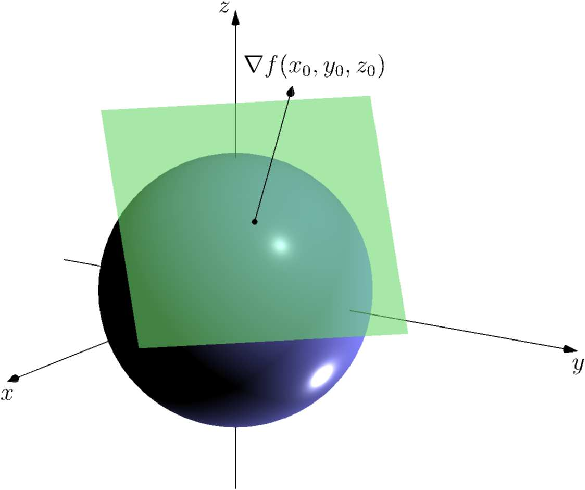
\includegraphics[width=\linewidth]{generated/asymptote/appltgsupniv.pdf}
\end{image}%
\tcblower
\end{figureptx}%
%
\par
Esta equação generaliza a situação anterior, quando a superfície é o gráfico de uma função de duas variáveis, \(f\colon
A\subseteq\mathbb R^2\to\R\). Basta ver que a superfície de nível \(0\) da função \(F(x,y,z)=f(x,y)-z\) é precisamente o gráfico de \(f\) e que, para todo \((x,y,z)\in F^{-1}(0)\), ou seja, \(z=f(x,y)\), temos \(\nabla
F(x,y,z)=\Big(f_x(x,y),f_y(x,y),-1\big)=n_f(x,y)\), de acordo com o que se segue após a \hyperref[definition-def_diff]{Definição~{\xreffont\ref{definition-def_diff}}}. É um bom exercício recuperar a equação presente naquela definição a partir da equação \hyperref[mrow-eq_pltgsupniv]{({\xreffont\ref{mrow-eq_pltgsupniv}})}.%
\begin{remark}{Nota}{}{remark-ap_supnivel-l}%
Observe que nem sempre uma curva de nível de uma função \(F\colon
A\subseteq\R^2\to\R\) é o gráfico de função \(f\colon
I\subseteq\R\to\R\). O mesmo ocorre para superfícies de nível de funções a três variáveis: a esfera acima é uma superfície de nível que não é gráfico de uma função a duas variáveis (por quê?).%
\end{remark}
Nos casos mais simples, quando as funções envolvidas são lineares, as curvas e superfícies de nível são, respectivamente, retas a planos, cujos vetores são normais são os gradientes das funções (constantes nesse caso). Tais retas ou planos são determinados resolvendo-se um sistema com uma equação e duas ou três variáveis. Para determinar, nesses sistemas, quais são as variáveis dependentes ou livres precisamos descobrir quais os coeficientes do vetor normal a esta reta ou plano são não nulos. Isso equivale à projeção da reta (respectivamente plano) de nível sobre os eixos das demais variáveis ser bijetora.%
\par
Se temos duas superfícies de nível, nesse caso mais simples planos, que não são paralelos ou coincidentes, sua interseção é uma reta. Os vetores normais de tais planos (os gradientes das funções lineares que os definem) são linearmente independentes e a direção da reta de interseção é justamente o produto vetorial desses vetores normais, já que a reta está contida em ambos os planos e portanto ortogonal aos dois vetores normais simultaneamente.%
\par
Algebricamente, encontrar esta reta consiste em resolver um sistema linear com duas equações e três variáveis. A condição para dizer quando uma das variáveis do sistema é a variável livre traduz-se na componente correspondente do vetor diretor da solução (o produto vetorial mencionado acima) ser não nula. Isso garante que a projeção da solução sobre o eixo coordenado daquela variável é bijetora.%
\par
Quando as funções envolvidas não são lineares, as curvas ou superfícies de nível deixam de ser retas ou planos, curvando-se de alguma maneira, consequentemente as soluções dos sistemas, agora não lineares, de ser retas ou planos, também curvando-se. A linearização dessa situação (considerando-se as retas tangentes às curvas de nível ou os planos tangentes às superfícies de nível) remontam aos parágrafos anteriores. Apresentamos a seguir três resultados que nos permitem, sob boas condições, escrever as retas tangentes a curvas de nível ou interseção de superfícies de nível, bem como planos tangente a uma superfície de nível.%
\begin{proposition}{Proposição}{Retas tangentes a curvas de nível.}{}{proposition-prop_curvaniv}%
Sejam \(F\colon A\subseteq\R^2\to\R\) uma função diferenciável no aberto \(A\) e \((x_0,y_0)\in A\) tal que \(F(x_0,y_0)=0\). Se existe uma função derivável \(f\colon
I\subseteq\R\to J\subset\R\), com \(x_0\in I\), \(y_0\in
J\), tal que \(y_0=f(x_0)\), \(F\big(x,f(x)\big)=0\) e \(F_y\big(x,f(x)\big)\neq 0\), para todo \(x\in I\), então%
\begin{equation*}
f'(x)=-\dfrac{F_x\big(x,f(x))}{F_y\big(x,f(x)\big)}.
\end{equation*}
\begin{remark}{Nota}{}{remark-prop_curvaniv-c}%
Caso tal \(f\) exista mesmo quando \(F_y(x_0,y_0)\), então devemos ter obrigatoriamente que \(f_x(x_0,y_0)=0\).\end{remark}
\end{proposition}
\begin{proof}{Demonstração}{}{proof-prop_curvaniv-d}
Suponha a existência de tal \(f\), podemos pensar na curva \(\gamma(x)=\big(x,f(x)\big)\), \(x\in I\) e usar a regra da cadeia (\hyperref[theorem-teo_cadeia]{Teorema~{\xreffont\ref{theorem-teo_cadeia}}}) para derivar a relação \(F(\big(x,f(x)\big)=0\), obtendo%
\begin{equation*}
0=\Big\langle\nabla
F\big(x,f(x)\big),\big(1,f'(x)\big)\Big\rangle\implies
F_x\big(x,f(x)\big)+F_y\big(x,f(x)\big)f'(x)=0.
\end{equation*}
%
\par
Como \(F_y\big(x,f(x)\big)\neq0\), temos a tese.%
\end{proof}
\begin{proposition}{Proposição}{Planos tangentes a superfícies de nível.}{}{proposition-prop_supniv}%
Sejam \(F\colon A\subseteq\R^3\to\R\) uma função diferenciável no aberto \(A\) e \((x_0,y_0,z_0)\in A\) tal que \(F(x_0,y_0,z_0)=0\). Se existe uma função derivável \(f\colon
B\subseteq\R^2\to J\subset\R\), com \((x_0,y_0)\in B\), \(z_0\in
J\), tal que \(z_0=f(x_0,y_0)\), \(F\big(x,y,f(x,y)\big)=0\) e \(F_z\big(x,y,f(x,y)\big)\neq 0\), para todo \(x\in I\), então%
\begin{equation*}
\dfrac{\partial f}{\partial
x}(x,y)=-\dfrac{F_x\big(x,y,f(x,y))}{F_z\big(x,y,f(x,y)\big)}\quad\text{e}\quad\dfrac{\partial
f}{\partial
y}(x,y)=-\dfrac{F_y\big(x,y,f(x,y))}{F_z\big(x,y,f(x,y)\big)}
\end{equation*}
\end{proposition}
\begin{proof}{Demonstração}{}{proof-prop_supniv-c}
A demonstração deste resultado é análoga à anterior, considerando agora duas curvas: para cada \(y\) fixado, \(\gamma_1(x)=\big(x,y,f(x,y)\big)\) e, para cada \(x\) fixado, \(\gamma_2(y)=\big(x,y,f(x,y)\big)\). Derive então, em relação a \(x\) e \(y\), respectivamente, as expressões \(F\big(\gamma_1(x)\big)=0\) e \(F\big(\gamma_2(y)\big)=0\).%
\end{proof}
\begin{proposition}{Proposição}{Retas tangentes a interseção de superfícies de nível.}{}{proposition-prop_intsupniv}%
Sejam \(F,G\colon A\subseteq\R^3\to\R\) funções diferenciáveis no aberto \(A\) e \((x_0,y_0,z_0)\in A\) tal que \(F(x_0,y_0,z_0)=0=G(x_0,y_0,z_0)\). Se existe uma função derivável \(\gamma\colon I\subseteq\R\to \R^3\), com \(x_0\in
I\) tal que \(\gamma(x_0)=(x_0,y_0,z_0)\), \(F\big(\gamma(x)\big)=0=G\big(\gamma(x)\big)\) e \(\det\begin{bmatrix}F_y&F_z\\G_y&
G_z\end{bmatrix}\big(\gamma(x)\big)\neq 0\), para todo \(x\in
I\), então%
\begin{equation*}
\gamma'(x)=\big(1,y'(x),z'(x)\big),
\end{equation*}
onde%
\begin{equation*}
y'(x)=-\dfrac{\det\begin{bmatrix}
F_x&F_z\\G_x&
G_z\end{bmatrix}\big(\gamma(x)\big)}
{\det\begin{bmatrix}
F_y&F_z\\G_y&
G_z\end{bmatrix}\big(\gamma(x)\big)}
\quad\text{e}
\quad z'(x)=-\dfrac{\det\begin{bmatrix}
F_y&F_x\\G_y&
G_x\end{bmatrix}\big(\gamma(x)\big)}
{\det\begin{bmatrix}
F_y&F_z\\G_y&
G_z\end{bmatrix}\big(\gamma(x)\big)}
\end{equation*}
\begin{remark}{Nota}{}{remark-prop_intsupniv-c}%
O determinante que pedimos ser não nulo nas hipóteses é o que garante que podemos ter a primeira componente de \(\gamma'(x)\) não nula, que é então paralelo vetor%
\begin{equation*}
\left(
\det\begin{bmatrix}
F_y&F_z\\G_y&
G_z\end{bmatrix},
\det\begin{bmatrix}
F_x&F_z\\G_x&
G_z\end{bmatrix},
\det\begin{bmatrix}
F_x&F_y\\G_x&
G_y\end{bmatrix}
\right)\big(\gamma(x)\big)
=(\nabla F\times\nabla
G)\big(\gamma(x)\big)\text{.}
\end{equation*}
\end{remark}
\end{proposition}
\begin{proof}{Demonstração}{}{proof-prop_intsupniv-d}
Temos aqui um sistema não linear com duas equações:%
\begin{equation*}
\begin{cases}
F\big(x,y(x),z(x)\big)&=0\\
G\big(x,y(x),z(x)\big)&=0.
\end{cases}
\end{equation*}
Derivando em relação a \(x\), com a regra da cadeia (\hyperref[theorem-teo_cadeia]{Teorema~{\xreffont\ref{theorem-teo_cadeia}}}), obtemos, para cada \(x\) fixado e omitindo os pontos de aplicação, um sistema \emph{linear} com duas equações nas incógnitas \(y'(x)\) e \(z'(x)\):%
\begin{equation*}
\begin{cases}
F_yy'(x)+F_zz'(x)&=-F_x\\
G_yy'(x)+G_zz'(x)&=-G_x.
\end{cases}
\end{equation*}
%
\par
Aplicando a \href{https://en.wikipedia.org/wiki/Cramer\%27s_rule\#Explicit_formulas_for_small_systems}{regra de Cramer}\footnotemark{} para a solução de sistemas lineares, temos as fórmulas do enunciado.%
\end{proof}
\footnotetext[2]{\nolinkurl{https://en.wikipedia.org/wiki/Cramer\%27s_rule\#Explicit_formulas_for_small_systems}\label{fn-prop_intsupniv-d-b-b}}%
Isto nos permite determinar a reta tangente a uma curva que é dada pela interseção de duas superfícies de nível, mesmo que não consigamos paramatrizá-la. Mas atenção: é \terminology{necessário} saber que tal interseção é uma curva derivável! Retomamos, como exemplo, o \hyperlink{exercise-curvasR3-2a}{Exercício~{\xreffont 1.8.2.a}}, para determinar a reta tangente à interseção das duas superfícies no ponto \((1,1,2,)\): consideramos \(F(x,y,z)=x^2+y^2-z\) e \(G(x,y,z)=2y-z\) que têm como superfícies de nível \(0\) aquelas do exercício. Seus gradientes são \(\nabla F(x,y,z)=(2x,2y,-1)\) e\(\nabla
G=(0,2,-1)\). Assim, o vetor diretor da reta pedida é um múltiplo não nulo de%
\begin{equation*}
\nabla F(1,1,2)\times \nabla
G(1,1,2)=(2,2,-1)\times(0,2,-1)=(0,2,4),
\end{equation*}
por exemplo \(\vec{v}=(0,1,2)\), e a reta tangente é \(r\colon
(x,y,z)=(1,1,2)+\lambda(0,1,2)\), \(\lambda\in\R\). \begin{figureptx}{Figura}{Interseções de superfícies de nível e sua reta tangente.}{figure-fig_appltgintsupniv}{}%
\begin{image}{0.25}{0.5}{0.25}{}%
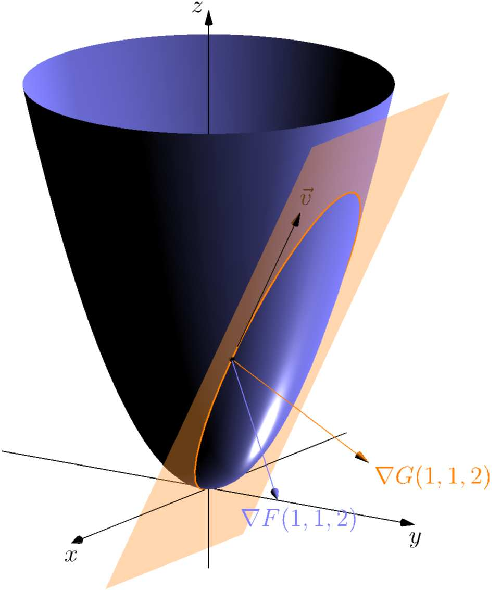
\includegraphics[width=\linewidth]{generated/asymptote/appltgintsupniv.pdf}
\end{image}%
\tcblower
\end{figureptx}%
%
\par
Os três resultados acima admitem \emph{recíprocas locais}, ou seja, se as funções que definemas as curvas ou superfícies de nível do enunciados são de classe \(\mathscr{C}^1\) (condição que pode ser relaxada) e as derivadas parciais não nulas dos enunciados acontecem num ponto da curva de nível, superfície de nível ou interseção de superfícies de nível, então é possível exibir uma vizinhança de tal objeto como gráfico de uma curva ou função, tambémm de classe \(\mathscr{C}^1\), com as derivadas dadas pelas fórmulas acima. Estes resultados são os celebrados Teoremas das Funções Implícitas, que admitem um enunciado unificado em contexto bem mais gerais. Um texto com demonstrações simples e muitos exemplos para as situações de interesse neste curso pode ser acessado \href{https://www.ime.usp.br/\~oliveira/ELE-IMPLI-EXEMPLOS.pdf}{aqui}\footnote{\nolinkurl{https://www.ime.usp.br/\~oliveira/ELE-IMPLI-EXEMPLOS.pdf}\label{fn-ap_supnivel-u-e}}. Agradecemos ao professor Oswaldo Rio Branco do IME-USP pelo excelente texto que preparou.%
\end{sectionptx}
%
%
\typeout{************************************************}
\typeout{Seção A.8 Máximos e mínimos locais em abertos de \(\R^2\)}
\typeout{************************************************}
%
\begin{sectionptx}{Seção}{Máximos e mínimos locais em abertos de \(\R^2\)}{}{Máximos e mínimos locais em abertos de \(\R^2\)}{}{}{section-ap_maxminloc}
\begin{introduction}{}%
Iniciamos agora o estudo dos máximos e mínimos locais de funções de várias variáveis reais. Neste primeiro momento vamos tratar a situação análoga ao que vimos no Cálculo 1 para pontos de máximo e mínimo em intervalos abertos: o \hyperref[theorem-teo_fermat]{Teorema~{\xreffont\ref{theorem-teo_fermat}}} e o teste da segunda derivada, dado no \hyperlink{exercise-teste_segder}{Exercício~{\xreffont 1.1.7}}.%
\par
Para tanto, estabelecemos as definições de ponts de máximos e mínimos (locais e globais) de uma função \(f\colon
A\subseteq\R^n\to\R\) (faremos com \(n=2\), mas tudo se generaliza funções de \(n\) variáveis a valores reais).%
\end{introduction}%
\begin{definition}{Definição}{}{definition-bola}%
A \terminology{bola aberta} de centro em \((x_0,y_0)\) e raio \(r>0\) de \(\R^2\) é o conjunto%
\begin{equation*}
B_r(x_0,y_0)=\big\{(x,y)\in\R^2\colon\|(x,y)-(x_0,y_0)\|<r\big\}.
\end{equation*}
\end{definition}
\begin{definition}{Definição}{}{definition-pto_maxmincrit}%
Sejam \(f\colon A\subseteq\R^2\to\R\) e \((x_0,y_0)\in
A\). Dizemos que%
\begin{itemize}[label=\textbullet]
\item{}\((x_0,y_0)\) é um \terminology{ponto de máximo local} de \(f\) se existe \(r>0\) tal que para todo \((x,y)\in
B_r(x_0,y_0)\bigcap A\), temos \(f(x,y)\leq
f(x_0,y_0)\).%
\item{}\((x_0,y_0)\) é um \terminology{ponto de mínimo local} de \(f\) se existe \(r>0\) tal que para todo \((x,y)\in
B_r(x_0,y_0)\bigcap A\), temos \(f(x,y)\geq
f(x_0,y_0)\).%
\item{}\((x_0,y_0)\) é um \terminology{ponto de máximo} (global) de \(f\) se \(f(x,y)\leq f(x_0,y_0)\) para todo \((x,y)\in A\).%
\item{}\((x_0,y_0)\) é um \terminology{ponto de mínimo} (global) de \(f\) se \(f(x,y)\geq f(x_0,y_0)\) para todo \((x,y)\in
A\).%
\end{itemize}
%
\par
Se \(f\) admite derivadas parciais em \((x_0,y_0)\) e \(\nabla f(x_0,y_0)=(0,0)\), então \((x_0,y_0)\) é um \terminology{ponto crítico de \(f\)}.%
\end{definition}
Assista ao vídeo abaixo para uma motivação dos resultados a seguir. \begin{figureptx}{Figura}{Máximos e mínimos locais.}{figure-vid_maxminloc}{}%
\begin{sidebyside}{2}{0.075}{0.075}{0.17}%
\begin{sbspanel}{0.47}%
\includegraphics[width=\linewidth]{generated/youtube/video-4.jpg}
\end{sbspanel}%
\begin{sbspanel}{0.21}%
\includegraphics[width=\linewidth]{generated/qrcode/video-4.png}
\end{sbspanel}%
\end{sidebyside}%
\tcblower
\end{figureptx}%
%
\begin{theorem}{Teorema}{}{}{theorem-teo_crit}%
Sejam \(A\subseteq\R^2\) um aberto contendo o ponto \((x_0,y_0)\) e \(f\colon A\to\R\) uma função que admite derivadas parciais em \((x_0,y_0)\). Se \((x_0,y_0)\) é um opnto de máximo ou mínimo local de \(f\), então \(\nabla
f(x_0,y_0)=(0,0)\).\end{theorem}
\begin{proof}{Demonstração}{}{proof-teo_crit-b}
Se \((x_0,y_0)\) é, digamos um ponto de máximo local, então \(x_0\) é ponto de máximo local de \(g(x)=f(x,y_0)\) num intervalo aberto \(I\), contendo o ponto \(x_0\). Segue-se então, do \hyperref[theorem-teo_fermat]{Teorema~{\xreffont\ref{theorem-teo_fermat}}} que%
\begin{equation*}
g'(x_0)=0\implies
f_x(x_0,y_0)=0.
\end{equation*}
%
\par
De maneira análoga, \(y_0\) é ponto de máximo local de \(h(y)=f(x_0,y)\), e então%
\begin{equation*}
h'(y_0)=0\implies f_y(x_0,y_0)=0.
\end{equation*}
%
 Ou seja, \(\nabla
f(x_0,y_0)=(0,0)\).\end{proof}
É importante mencionar que a recíproca do teorema acima, assim como visto na nota do \hyperref[theorem-teo_fermat]{Teorema~{\xreffont\ref{theorem-teo_fermat}}} para o caso de uma veriável, é falsa: considere \(f(x,y)=x^2-y^2\), definida em todo o plano \(\R^2\) (um aberto). Temos que \(\nabla f(0,0)=(0,0)\) e este não é um ponto de máximo local, nem de mínimo local, já que \(f(0,y)< f(0,0) < f(x,0)\), para quaisquer \((x,y)\neq
(0,0)\).%
\par
Um ponto crítico, no domínio de uma função, que não é de máximo local nem de mínimo local é chamado de \terminology{ponto de sela} daquela função. A nomenclatura vem da semelhança do gráfico da função acima com uma sela. Veja a \hyperref[figure-fig_parabhip3d]{Figura~{\xreffont\ref{figure-fig_parabhip3d}}}.%
\par
A fim de tentar generalizar o \emph{teste da segunda} para classificar os pontos críticos de funções de duas variáveis, precisamos levar em conta as quatro segundas derivadas e aplicar técnica análoga à empregada no \hyperlink{exercise-teste_segder}{Exercício~{\xreffont 1.1.7}}. Para isso apresentamos rapidamente a fórmula de Taylor para funções de classe \(\mathscr{C}^2\) a duas variáveis reais.%
\begin{theorem}{Teorema}{(Fórmula de Taylor).}{}{theorem-ap_maxminloc-j}%
Sejam \(f\colon A\subseteq\R^2\to\R\) de classe \(\mathscr{C}^2\) no ponto \((x_0,y_0)\) do convexo \(A\). Então%
\begin{equation*}
f(x,y)=f(x_0,y_0)+f_x(x_0,y_0)(x-x_0)+f_y(x_0,y_0)(y-y_0)+E(x,y),
\end{equation*}
onde%
\begin{equation*}
E(x,y)=\dfrac{1}{2}\Big(f_{xx}(\overline{x},\overline{y})(x-x_0)^2+2f_{xy}(\overline{x},\overline{y})(x-x_0)(y-y_0)+f_{yy}(\overline{x},\overline{y})(y-y_0)^2\Big),
\end{equation*}
com \((\overline{x},\overline{y})\) no segmento ligando \((x_0,y_0)\) a \((x,y)\).\end{theorem}
\begin{proof}{Demonstração}{}{proof-ap_maxminloc-j-c}
Basta aplicar a fórmula de Taylor de uma variável real, centrada em \(t_0=0\), para a função%
\begin{equation*}
g(t)=f\big(\gamma(t)\big),
\end{equation*}
com \(\gamma(t)=\big(x(t),y(t)\big)=(x_0,y_0)+t(x-x_0,y-y_0)\), para \(t\) num intervalo abeto contendo \([0,1]\) tal que a imagem de \(\gamma\) esteja contida em \(A\).%
\par
Assim, temos \(g(0)=f(x_0,y_0)\) e, aplicando a regra da cadeia sucessivas vezes, que%
\begin{align*}
g'(0)&=\big\langle\nabla
f(x_0,y_0),(x-x_0,y-y_0)\big\rangle=f_x(x_0,y_0)(x-x_0)+f_y(x_0,y_0)(y-y_0)\\
g''(t)&=\Big(f_{xx}\big(\gamma(t)\big)(x-x_0)^2+
2f_{xy}\big(\gamma(t)\big)(x-x_0)(y-y_0)+
f_{yy}\big(\gamma(t)\big)(y-y_0)^2\Big)
\end{align*}
%
\par
Logo,%
\begin{equation*}
g(1)=g(0)+g'(0)(1-0)+\dfrac{g''(\overline{t})}{2}(1-0)^2,\quad
\overline{t}\in ]0,1[,
\end{equation*}
ou seja, a fórmula apresentada no enunciado, onde \((\overline{x},\overline{y})=\gamma(\overline{t})\).%
\end{proof}
Com isso podemos apresentar o chamado \terminology{critério do Hessiano}:%
\begin{theorem}{Teorema}{}{}{theorem-teo_hess}%
Sejam \(A\subseteq\R^2\) um aberto e \((x_0,y_0)\in A\) um ponto crítico da função \(f\colon A\to\R\), de classe \(\mathscr{C}^2\) em \((x_0,y_0)\). Se %
\begin{enumerate}[label=(\roman*)]
\item{}\(\det H_f(x_0,y_0)> 0\) e \(f_{xx}(x_0,y_0)>
0\), então \((x_0,y_0)\) é um ponto de mínimo local de \(f\).%
\item{}\(\det H_f(x_0,y_0)> 0\) e \(f_{xx}(x_0,y_0)<
0\), então \((x_0,y_0)\) é um ponto de máximo local de \(f\).%
\item{}\(\det H_f(x_0,y_0)< 0\) então \((x_0,y_0)\) é um ponto de sela de \(f\).%
\end{enumerate}
 Aqui \(H_f(x_0,y_0)=\begin{bmatrix} f_{xx}(x_0,y_0)&
f_{yx}(x_0,y_0)\\ f_{xy}(x_0,y_0)& f_{yy}(x_0,y_0)\\
\end{bmatrix}\) é a \terminology{matriz Hessiana} de \(f\) em \((x_0,y_0)\).\begin{remark}{Nota}{}{remark-teo_hess-c}%
Note que este resultado nada afirma no caso em que \(\det
H_f(x_0,y_0)=0\). Tais casos devem ser estudados de maneira "artesanal".\end{remark}
\end{theorem}
\begin{proof}{Demonstração}{}{proof-teo_hess-b}
Veja \href{./external/classif-ptos-crit.pdf}{aqui}\footnotemark{}.\end{proof}
\footnotetext[1]{\nolinkurl{./external/classif-ptos-crit.pdf}\label{fn-teo_hess-b-b}}%
\end{sectionptx}
%
%
\typeout{************************************************}
\typeout{Seção A.9 Máximos e mínimos condicionados}
\typeout{************************************************}
%
\begin{sectionptx}{Seção}{Máximos e mínimos condicionados}{}{Máximos e mínimos condicionados}{}{}{section-ap_maxmincond}
\begin{introduction}{}%
Agora vamos tratar do caso análogo ao do estudo de máximos e mínimo de funções de uma variável real em intervalos fechados. Começamos estabelecendo uma generalização para intervalos em domínios de dimensão mais alta.%
\end{introduction}%
\begin{definition}{Definição}{}{definition-compacto}%
Um conjunto \(A\subseteq\R^n\) é \terminology{compacto} se for fechado e limitado. Por \terminology{fechado} entendemos um conjunto cujo complementar é aberto (todos os pontos de um aberto são pontos interiores, ou seja, centros de bolas abertas inteiramente contidas nele). Um conjunto é \terminology{limitado} se existe uma bola aberta centrada na origem que o contém.\end{definition}
Como no Cálculo 1, temos o%
\begin{theorem}{Teorema}{}{}{theorem-teo_wei}%
Se \(f\colon A\subseteq\R^2\to\R\) é uma função contínua no compacto \(A\) então existem \((x_0,y_0)\) e \((x_1,y_1)\) em \(A\) tais que%
\begin{equation*}
f(x_0,y_0)\leq
f(x,y)\leq f(x_1,y_1).
\end{equation*}
%
\par
Em outras palavras, toda função contínua definida num compacto assume valores máximo e mínimo (globais).%
\end{theorem}
A prova deste resultado é um tanto técnica e pode ser negligenciada (momentaneamente).%
\begin{example}{Exemplo}{}{example-ap_maxmincond-g}%
Decida se a função \(f(x,y)=xy\), definida no conjunto \(A=\big\{(x,y)\in\R^2\colon x^2+y^2\leq 1\big\}\) admite valor máximo ou mínimo. Em caso afirmativo determine os pontos onde isso ocorre.\par\smallskip%
\noindent\textbf{\blocktitlefont Solução}.\hypertarget{solution-ap_maxmincond-g-b}{}\quad{}Observamos que \(f\) é contínua (mais que isso até) e o conjunto \(A\) é compacto. Pelo \hyperref[theorem-teo_wei]{Teorema~{\xreffont\ref{theorem-teo_wei}}} acima, temos que a função assume valor máximo e também valor mínimo em \(A\).%
\par
Para determinar os pontos onde isso ocorre, notamos que o conjunto \(A\) tem interior não vazio, que é o disco "aberto" \(\big\{(x,y)\in\R^2\colon x^2+y^2< 1\big\}\),  e uma fronteira não vazia, que é a circunferência \(\big\{(x,y)\in\R^2\colon
x^2+y^2= 1\big\}\). No interior, os candidatos a máximo e mínimo são determinados usando-se o \hyperref[theorem-teo_crit]{Teorema~{\xreffont\ref{theorem-teo_crit}}}:%
\begin{equation*}
\nabla
f(x,y)=(y,x)=(0,0)\iff (x,y)=(0,0),
\end{equation*}
onde temos \(\boxed{f(0,0)=0}\).%
\par
A fronteira, neste caso especial, pode ser parametrizada por \(\gamma(t)=(\cos t, \sin t)\), \(t\in [0,2\pi]\). Sobre os pontos da froteira temos que \(f\) se comporta como%
\begin{equation*}
f\big(\gamma(t)\big)=\cos t \sin t, \quad t\in [0,2\pi],
\end{equation*}
que é uma função contínua de uma variável real definida num intervalo fechado. Sabemos o que fazer!%
\par
Se \(t_0\) é ponto de máximo ou mínimo de \(f\big(\gamma(t)\big)\) no interior do intervalo, devemos ter \((f\circ\gamma)'(t_0)=0\). Nesse caso podemos calcular explicitamente:%
\begin{equation*}
(f\circ\gamma)'(t_0)=0\iff\cos(2t)=0\iff
t=\dfrac{k\pi}{4}, k=1,3,5,7.
\end{equation*}
Anotamos os valores nesses pontos:%
\begin{equation*}
f\big(\gamma(\pi/4)\big)=\boxed{f(\sqrt{2}/2,\sqrt{2}/2)=1/2=f(-\sqrt{2}/2,-\sqrt{2}/2)}=f\big(\gamma(5\pi/4)\big)
\end{equation*}
%
\begin{equation*}
f\big(\gamma(3\pi/4)\big)=\boxed{f(-\sqrt{2}/2,\sqrt{2}/2)=-1/2=f(\sqrt{2}/2,-\sqrt{2}/2)}=f\big(\gamma(7\pi/4)\big)
\end{equation*}
%
\par
Comparando os valores em destaque temos que o valor máximo de \(f\) em \(A\) é \(1/2\) e o mínimo é \(-1/2\), atingidos nos pontos indicados acima. O ponto \((0,0)\) é um candidato onde a função não atingiu seu valor máximo nem seu valor mínimo (você já sabia isso da seção anterior).%
\par
Note que se usássemo a regra da cadeia para derivar \(f\circ\gamma\), observaríamos que os candidatos a máximo e mínimo são aqueles onde o gradiente de \(f\) é ortogonal a \(\gamma'\). Guarde isso!%
\end{example}
Considerando o exemplo acima (principalmente a observação ao final da solução), assista o vídeo abaixo para motivar os resultados seguintes. \begin{figureptx}{Figura}{Máximos e mínimos condicionados.}{figure-vid_maxmincond}{}%
\begin{sidebyside}{2}{0.075}{0.075}{0.17}%
\begin{sbspanel}{0.47}%
\includegraphics[width=\linewidth]{generated/youtube/video-5.jpg}
\end{sbspanel}%
\begin{sbspanel}{0.21}%
\includegraphics[width=\linewidth]{generated/qrcode/video-5.png}
\end{sbspanel}%
\end{sidebyside}%
\tcblower
\end{figureptx}%
%
\par
Agora estamos em condições de enunciar os resultados sobre máximos e mínimos de funções a várias (duas ou três) variáveis com restrições dadas por conjuntos de nível ou interseções deles.%
\begin{theorem}{Teorema}{}{}{theorem-teo_lag2}%
Sejam \(f,g\colon A\subseteq\R^2\to\R\) de classe \(\mathscr{C}^1\) e \(B=\big\{(x,y)\in A\colon
g(x,y)=0\big\}\), com \(\nabla g(x,y)\neq 0\), para todo \((x,y)\in B\). Se \((x_0,y_0)\in B\) é um ponto de máximo ou mínimo local de \(f\) sobre \(B\) (detalhes do que é isso ficam claros na demonstração), então \(\big\{\nabla
f(x_0,y_0),\nabla g(x_0,y_0)\big\}\) é um conjunto linearmente dependente.\begin{remark}{Nota}{}{remark-teo_lag2-c}%
Lembramos que \(\{\vec{u},\vec{v}\}\) é linearmente dependente em \(\R^2\) se, e somente se, a matriz \(2\times
2\), com as coordenadas de tais vetores nas linhas, tem determinante nulo.\end{remark}
\end{theorem}
\begin{proof}{Demonstração}{}{proof-teo_lag2-b}
Apresentamos aqui apenas um esboço da demonstração. Como, em particular, \(\nabla g(x_0,y_0)\neq 0\), e \(g\) é de classe \(\mathscr{C}^1\), usamos o Teorema da Função Implícita (veja \hyperref[proposition-prop_curvaniv]{Proposição~{\xreffont\ref{proposition-prop_curvaniv}}} e a observação sobre sua recíproca ao fim daquela seção) para exibir uma curva de classe \(\mathscr{C}^1\), \(\gamma\colon I\to\R^2\), com \(I\) um intervalo aberto contendo \(t_0\) tal que \(\gamma(t_0)=(x_0,y_0)\). Sabemos, inclusive, que tal curva é o gráfico de \(y\) como função de \(x\) ou vice-versa).%
\par
Tratamos aqui apenas o caso de máximo local (o outro é análogo). Sendo \((x_0,y_0)\in B\) é um ponto de máximo local de \(f\) sobre \(B\), ou seja, \(f\big(\gamma(t_0)\big)=f(x_0,y_0)\geq f\big(\gamma(t)\big)\) para todo \(t\in J\), onde \(J\) é um intervalo aberto que contém \(t_0\) e está contido em \(I\), temos que%
\begin{equation*}
(f\circ\gamma)'(t_0)=0\iff \langle\nabla
f(x_0,y_0),\gamma'(t_0)\rangle=0\iff \boxed{\nabla
f(x_0,y_0)\perp\gamma'(t_0)}.
\end{equation*}
%
\par
Agora, como \(\gamma\) parametriza uma parte da curva de nível \(0\) de \(g\) então, do \hyperref[corollary-cor_cadeiagradniv]{Corolário~{\xreffont\ref{corollary-cor_cadeiagradniv}}}, temos que \(\boxed{\nabla g(x_0,y_0)\perp\gamma'(t_0)}\). As duas expressões em destaque garantem, uma vez que estamos em \(\R^2\), que%
\begin{equation*}
\nabla f(x_0,y_0)\parallel\nabla
g(x_0,y_0)\text{,}
\end{equation*}
como desejado.%
\end{proof}
Uma outra maneira de enxergar esse resultado é que, num ponto de máximo ou de mínimo de \(f\) sobre uma curva de nível de \(g\), a projeção de \(\nabla f\) na direção tangente à tal curva de nível é nula. Em outras palavras, alguém que se desloca sobre a curva de nível de \(g\) "não sente" as derivadas de \(f\) quando passa por um de seus pontos de máximo ou mínimo.%
\par
Importante ressaltar que, como já estamos acostumados, não vale a recíproca, ou seja, se os gradientes são paralelos num ponto, não temos garantia que esse ponto é um de máximo ou mínimo local sobre aquela restrição.%
\par
Um exemplo interessante onde o teorema ajuda, mas não é suficiente para encontrar a solução está \href{./external/lagrange.pdf}{aqui}\footnote{\nolinkurl{./external/lagrange.pdf}\label{fn-ap_maxmincond-m-b}}.%
\par
De maneira análoga, o resultado acima vale para máximos ou mínimos locais de funções a três variáveis sobre uma superfície de nível de outra função:%
\begin{theorem}{Teorema}{}{}{theorem-teo_lag31}%
Sejam \(f,g\colon A\subseteq\R^3\to\R\) de classe \(\mathscr{C}^1\) e \(B=\big\{(x,y,z)\in A\colon
g(x,y,z)=0\big\}\), com \(\nabla g(x,y,z)\neq 0\), para todo \((x,y,z)\in B\). Se \((x_0,y_0,z_0)\in B\) é um ponto de máximo ou mínimo local de \(f\) sobre \(B\), então \(\big\{\nabla f(x_0,y_0,z_0),\nabla g(x_0,y_0,z_0)\big\}\) é um conjunto linearmente dependente.\begin{remark}{Nota}{}{remark-teo_lag31-c}%
Lembramos que \(\{\vec{u},\vec{v}\}\) é linearmente dependente em \(\R^3\) se, e somente se, o produto vetorial \(\vec{u}\wedge\vec{v}=\vec{0}\).\end{remark}
\end{theorem}
\begin{proof}{Demonstração}{}{proof-teo_lag31-b}
A ideia aqui é essencialmente a mesma que a da proposição anterior, observando que \((f\circ\gamma)'(t_0)=0\) para toda curva \(\gamma\) cuja imagem está contida na superfície de nível \(0\) de \(g\), \(B=g^{-1}(0)\).%
\par
Isso mostra, como visto na \hyperref[definition-def_planotangente]{Definição~{\xreffont\ref{definition-def_planotangente}}}, que \(\nabla f(x_0,y_0,z_0)\) é ortogonal ao plano tangente à \(B\) em \((x_0,y_0,z_0)\), assim como \(\nabla
g(x_0,y_0,z_0)\) é ortogonal ao plano tangente à \(B\) nesse ponto. Dois vetores de \(\R^3\) ortogonais a uma mesmo plano devem ser paralelos.%
\end{proof}
Finalmente, estabelecemos o resultado para pontos de máximo ou mínimo local sobre a interseção de duas superfícies de nível de duas outras funções:%
\begin{theorem}{Teorema}{}{}{theorem-teo_lag32}%
Sejam \(f,g,h\colon A\subseteq\R^3\to\R\) de classe \(\mathscr{C}^1\) e%
\begin{equation*}
B=\big\{(x,y,z)\in A\colon
g(x,y,z)=h(x,y,z)=0\big\}\text{,}
\end{equation*}
com \(\nabla g(x,y,z)\wedge\nabla
h(x,y,z)\neq\vec{0}\), para todo \((x,y,z)\in B\). Se \((x_0,y_0,z_0)\in B\) é um ponto de máximo ou mínimo local de \(f\) sobre \(B\), então \(\big\{\nabla
f(x_0,y_0,z_0),\nabla g(x_0,y_0,z_0),\nabla
h(x_0,y_0,z_0)\big\}\) é um conjunto linearmente dependente.\begin{remark}{Nota}{}{remark-teo_lag32-c}%
Lembramos que \(\{\vec{u},\vec{v},\vec{w}\}\) é linearmente dependente em \(\R^3\) se, e somente se, o produto misto \([\vec{u},\vec{v},\vec{w}]=\langle
\vec{u}\wedge\vec{v},\vec{w}\rangle=0\).\end{remark}
\end{theorem}
\begin{proof}{Demonstração}{}{proof-teo_lag32-b}
Nada inédito: como \(g\) e \(h\) são de classe \(\mathscr{C}^1\), a condição \(\nabla
g(x_0,y_0,z_0)\wedge\nabla h(x_0,y_0,z_0)\neq\vec{0}\) garante, através do Teorema da Função Implícita, a existência de uma função de classe \(\mathscr{C}^1\), \(\gamma\colon I\to\R^3\), onde \(I\) é um intervalo aberto contendo \(t_0\) tal que \(\gamma(t_0)=(x_0,y_0,z_0)\) e \(\gamma(t)\in
B=g^{-1}(0)\bigcap h^{-1}(0)\). Já sabemos que%
\begin{equation*}
\gamma'(t)\parallel \nabla g\big(\gamma(t)\big)\wedge\nabla
h\big(\gamma(t)\big)\text{.}
\end{equation*}
%
\par
Se \((x_0,y_0,z_0)\) é máximo (ou mínimo) local de \(f\) ao longo de \(B\), então%
\begin{equation*}
(f\circ\gamma)'(t_0)=0\iff
\langle\nabla f(x_0,y_0),\gamma'(t_0)\rangle=0\iff \boxed{\nabla
f(x_0,y_0,z_0)\perp\gamma'(t_0)}.
\end{equation*}
%
\par
A condição destacada acima, e a hipótese inicial sobre independência linear dos gradientes de \(g\) e \(h\), garantem que%
\begin{equation*}
\nabla f(x_0,y_0,z_0)\in\big[\nabla
d(x_0,y_0,z_0),\nabla h(x_0,y_0,z_0)\big]\text{,}
\end{equation*}
ou seja, \(\big\{\nabla f(x_0,y_0,z_0)m\nabla f(x_0,y_0,z_0),\nabla
f(x_0,y_0,z_0)\big\}\) é linearmente dependente, como desejado.%
\end{proof}
\end{sectionptx}
\end{appendixptx}
%
\backmatter%
%
\clearpage\phantomsection%
\addcontentsline{toc}{part}{Pós-textual}%
\clearpage
\pagestyle{empty}
\vspace*{\stretch{1}}
\begin{backcolophon}{Ficha técnica}{colophon-meta_backmatter-c}%
Este material foi preparado utilizando o PreTeXt.%
\end{backcolophon}%
\vspace*{\stretch{2}}
\end{document}
